% !TeX program = lualatex

\documentclass[manuscript,screen,review,anonymous]{acmart}

%TODO: check compliance
%  ==================== MY PACKAGES ====================
\usepackage{graphicx}
\usepackage{multirow}
\usepackage{pifont}
\usepackage{booktabs}
\usepackage{float}
\usepackage{acronym}
\usepackage{tabularx}
\usepackage{hyperref}
\usepackage{url}
\usepackage{colortbl}
\usepackage{siunitx}
\usepackage{multicol}
\usepackage{longtable}
\usepackage{censor}
\usepackage[inline]{enumitem}
\usepackage{wasysym}

%  ==================== MY COMMANDS ====================
\AtEndPreamble{%
	\newtheorem{hypothesis}{Hypothesis}
	
	\theoremstyle{acmplain}
	\newtheorem{finding}{Finding}
	
	\newtheoremstyle{researchquestionstyle}
	{} % Space above
	{} % Space below
	{\normalfont} % Body font: Use normal/upright font for the main text
	{} % Indent amount
	{} % Head font: Use bold font for the title and optional argument
	{?} % Punctuation after head
	{ } % Space after theorem head
	{\thmname{#1}\thmnumber{ #2}:\thmnote{ \emph{#3}}}
	\theoremstyle{researchquestionstyle}
	\newtheorem{researchquestion}{RQ}
}


\newcommand{\warning}[1]{\textcolor{ACMRed}{\textbf{#1}}}
\newcommand{\sigyes}{\checked}
\newcommand{\signo}{$\times$}
\newcommand{\librarylink}{ \url{https://anonymous.4open.science/r/apunim-5F70}}
\newcommand{\doclink}{\url{https://anonymous.4open.science/r/apunim-page}}
\newcommand{\explink}{\url{https://anonymous.4open.science/r/aposteriori-unimodality-E8C1}}

\newcommand\given[1][]{\:#1\vert\:}

\graphicspath{ {../graphs} {graphs} }

\title[Quantifying and Auditing Group-Based Disagreement]{Quantifying and Auditing Group-Based Disagreement in Human and LLM Annotation}

\author{Anonymous}


\begin{document}

\begin{abstract}
	LLM annotation is increasingly used as a scalable substitute for human annotations, including in polarized, subjective tasks where humans systematically disagree along group lines. Whether these systems reproduce, ignore, or distort human disagreement patterns is largely untested, in part because most existing methods for attributing \ac{sysdis} have not yet been tested in realistic, subjective annotation settings. This work represents the first empirical study which applies proposed, theoretical methods on large scale, realistic annotation settings. Observing the weaknesses of these methods, we develop a method that not only detects, but also quantifies attribution of \ac{sysdis} to annotator sociodemographic \acp{sdd} and use it to audit nine open-source LLMs against five real-life datasets on subjective \ac{nlp} tasks. Our results show that while persona-prompted LLMs can produce polarized annotations, the exhibited disagreement patterns are not aligned with those of human annotator \acp{sdd}, even when tuning instruction prompts for this purpose. This limitation indicates that applications, studies and resources using persona prompting should include appropriate scoping and evaluation in order to avoid further model miscalibration. Our study also suggests that the structure of current subjective NLP datasets is insufficient, requiring more annotators per item, as we find that not all \ac{sysdis} can be attributed to any combination of known or latent annotator \acp{sdd}.
\end{abstract}

\begin{CCSXML}
	<ccs2012>
	<concept>
	<concept_id>10010147.10010178.10010179</concept_id>
	<concept_desc>Computing methodologies~Natural language processing</concept_desc>
	<concept_significance>500</concept_significance>
	</concept>
	<concept>
	<concept_id>10010147.10010257.10010258.10010260</concept_id>
	<concept_desc>Computing methodologies~Unsupervised learning</concept_desc>
	<concept_significance>500</concept_significance>
	</concept>
	<concept>
	<concept_id>10003120.10003130.10011762</concept_id>
	<concept_desc>Human-centered computing~Empirical studies in collaborative and social computing</concept_desc>
	<concept_significance>500</concept_significance>
	</concept>
	<concept>
	<concept_id>10003456.10010927.10003611</concept_id>
	<concept_desc>Social and professional topics~Race and ethnicity</concept_desc>
	<concept_significance>300</concept_significance>
	</concept>
	<concept>
	<concept_id>10003456.10010927.10003613</concept_id>
	<concept_desc>Social and professional topics~Gender</concept_desc>
	<concept_significance>300</concept_significance>
	</concept>
	<concept>
	<concept_id>10003456.10010927.10003614</concept_id>
	<concept_desc>Social and professional topics~Sexual orientation</concept_desc>
	<concept_significance>100</concept_significance>
	</concept>
	<concept>
	<concept_id>10003456.10010927.10010930</concept_id>
	<concept_desc>Social and professional topics~Age</concept_desc>
	<concept_significance>100</concept_significance>
	</concept>
	<concept>
	<concept_id>10010147.10010178.10010179.10010186</concept_id>
	<concept_desc>Computing methodologies~Language resources</concept_desc>
	<concept_significance>100</concept_significance>
	</concept>
	</ccs2012>
\end{CCSXML}

\ccsdesc[500]{Computing methodologies~Natural language processing}
\ccsdesc[500]{Computing methodologies~Unsupervised learning}
\ccsdesc[500]{Human-centered computing~Empirical studies in collaborative and social computing}
\ccsdesc[300]{Social and professional topics~Race and ethnicity}
\ccsdesc[300]{Social and professional topics~Gender}
\ccsdesc[100]{Social and professional topics~Sexual orientation}
\ccsdesc[100]{Social and professional topics~Age}
\ccsdesc[100]{Computing methodologies~Language resources}

\keywords{Polarization, Clustering, Annotation, Sociodemographic Characteristics, Persona-Prompting}

\maketitle


\section{Introduction}
\label{sec:intro}

\begin{figure}[t]
	\centering
	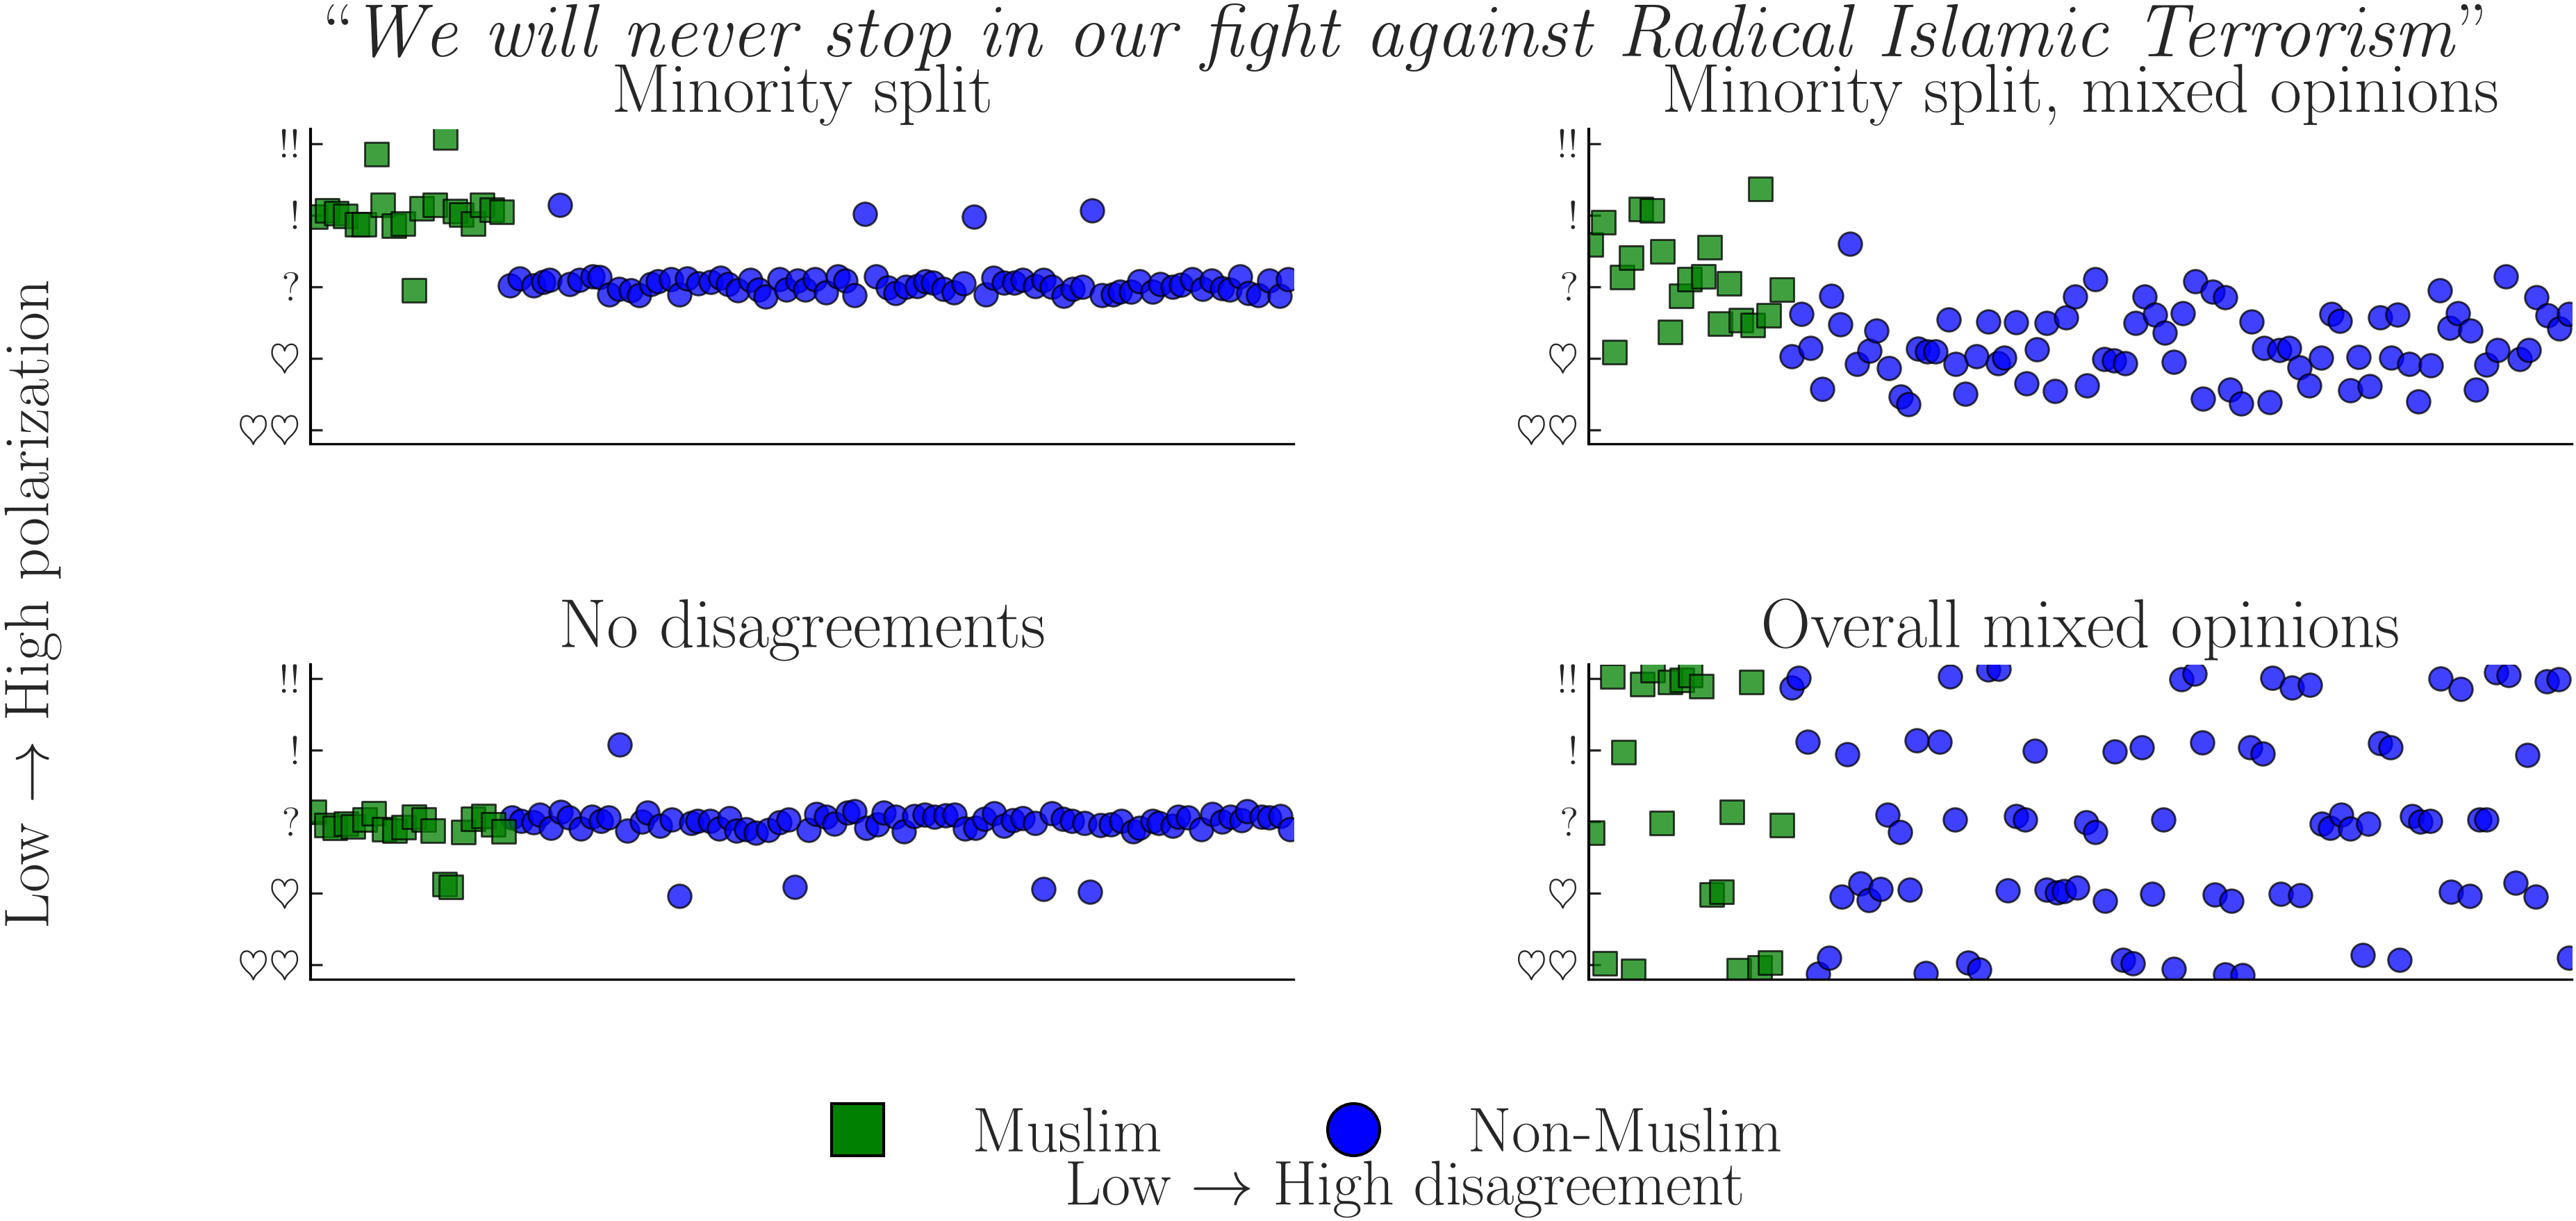
\includegraphics[width=\linewidth]{disagreement_vs_polarization.png}
	\caption{Simulated experiment exploring four scenarios of a \ac{hs} detection task applied to a controversial statement. The variance in annotations across different annotators may cause traditional \ac{iaa} measures to ignore minority opinions, especially when opinions are mixed (top-right).}
	\label{fig:disagreement-vs-polarization}
\end{figure}

\acresetall

The rise of internet spaces has necessitated research in subjective phenomena such as the detection of harmful content. Annotations are needed to support social science research, the training of automated classifiers and the proactive identification of vulnerable groups \citep{vidgen_2021_directions}. These annotations are frequently released as datasets, which due to their subjective nature typically contain items with very low \ac{iaa} \citep{vidgen_2021_directions}. If ignored, this disagreement may lead to loss of valuable information \citep{pavlopoulos-likas-2024} and provide us with the wrong signal, leading to significant misconfiguration in trained AI systems \citep{uma2021}. For example, toxicity models have disproportionately marked \ac{aa} speech as ``toxic'' \citep{sap-etal-2019-risk}, or systematically ignored minority opinions \citep{quaranto2022dog} in the past.

In practice, researchers usually use \ac{iaa} measures to distinguish between general and \ac{sysdis} (Fig.~\ref{fig:disagreement-vs-polarization}). Traditional measures however hold significant limitations, especially when few annotations per item are available and when the studied \acp{sdd} contain imbalanced groups. Both of these issues are typically present in subjective tasks featuring minorities, which is the exact case where our measures should be reliable. Furthermore, as human annotation is generally expensive, LLM-as-judge systems are increasingly deployed as scalable substitutes for human annotators \citep{rossi_2024, kapania-etal-2025-examining} to acquire a cheaper, ``bronze'' supervision signal in place of human-annotated ``silver'' or ``gold'' labels. It is therefore imperative that \ac{sysdis} by human annotators be preserved by LLMs whose annotations by default gravitate toward the statistical average \citep{bisbee_2023}. Persona-prompting is sometimes used to bypass this limitation, but suffers from its own challenges such as stereotyping and inconsistent annotations \citep{lutz-etal-2025-prompt, liu-etal-2024-evaluating-large}. We therefore ask:

\begin{researchquestion}[How Do Current Theoretical Polarization Attribution Approaches Behave in Realistic Annotation Scenarios]
	Our work is the first empirical study applying measures of polarization detection and attribution in real-life subjective datasets. We find that these theoretical models tend to collapse, while \ac{iaa} underperforms. One of the reasons for this collapse is likely the assumption that annotations can be aggregated across items (Finding~\ref{finding:methods}).
\end{researchquestion}

\begin{researchquestion}[How Can \ac{sysdis} be Quantitatively Attributed to Annotator \acp{sdd}]
	\label{rq:measure}
	We introduce a new measure which \emph{quantitatively} attributes \ac{sysdis} to specific \acp{sdd}, while being conscious of the limitations present in realistic annotation scenarios (Fig.~\ref{fig:measures}). 
\end{researchquestion}

\begin{researchquestion}[Which \ac{sysdis} Patterns are Shared Between Human and LLM Annotators]
	\label{rq:llm}
	Unlike prior work which framed the question of LLM annotation reliability in terms of human-LLM agreement \citep{dong-etal-2024-llm, gomez-etal-2024-algorithmic, masud-etal-2024-hate} or task-specific performance \citep{gupta2024bias}, we compare human and LLM polarization patterns. We find that human \ac{sysdis} is attributed to gender and ethnicity across five real-life subjective datasets (Finding~\ref{finding:human}). On the other hand, while LLMs using persona-prompting \emph{can} produce polarized annotations, they fail to reproduce any \ac{sysdis} patterns regardless of instruction prompt, confirming literature suggesting that persona prompting does not consistently influence LLM outputs in the examined tasks (Finding~\ref{finding:llms}).
\end{researchquestion}

Overall, our work indicates that persona-prompting requires extensive evaluation and careful scoping as it may compromise sensitive applications (e.g., content moderation, facilitation), contaminate LLM training and lead to misleading findings in social science research . It also argues for a paradigm shift in the design and construction of subjective datasets; the true limit in current datasets should not the number of annotated items, but rather the number of annotations per item (\S\ref{sec:discussion}). Indeed, we find the existence of ``\ac{unpol}'' which can not be explained by any possible combination of \acp{sdd} known or unknown, and likely stems from annotation sparsity on the item level (Finding~\ref{finding:inherent}).

Finally, we release a PyPI library implementing our measure to aid future research in this topic.  All code, environment details, data-processing scripts and our library are released anonymously: library \librarylink, HTML documentation \doclink, replication code \explink. 

\makeatletter
\AC@reset{unpol}
\makeatother

\begin{center}
	\noindent\warning{Content Warning: Controversial and potentially harmful speech used for demonstration purposes only.}
\end{center}


\section{Background and Related Work}
\label{sec:related}

\paragraph{Terminology} We distinguish three definitions used throughout this work:
\begin{enumerate*}
	\item \textbf{Disagreement} represents any variance among annotators' ratings for the same item, regardless of its source.
	\item  \textbf{\ac{sysdis}} is non-random and recurring disagreement, which in this work is assumed to be caused by differences in group identity (e.g., background, cultural context, ideology).
	\item  \textbf{Polarization} is the underlying societal phenomenon describing genuinely conflicting, opposed viewpoints on the same item.
\end{enumerate*}
Specifically, we attempt to find \emph{polarized} \acp{sdd} through the distinction of \emph{\ac{sysdis}} from general \emph{disagreement} in annotations.

\paragraph{Inter-Annotator Agreement} Current research on analyzing subjective tasks mostly rests on using \ac{iaa} between groups of a single annotator \ac{sdd}~\citep{davani-etal-2022-dealing, leonardelli-etal-2023-semeval, uma_2022_scaling, ivey-etal-2025-nutmeg, petra_2022_handling, van_der_Velden}, as prior work has shown that consistent, \ac{sysdis} may be caused by different points-of-view between groups \citep{davani-etal-2022-dealing, uma2021, goyal2022your}. \ac{iaa} measures such as Cohen's kappa, Krippendorff's alpha, and Fleiss's kappa aim to distinguish genuine disagreement from random disagreement through statistical chance-correction. However, these measures are often difficult to apply to intergroup \ac{iaa} without extensions or restrictive assumptions (e.g., no missing labels or equal numbers of annotations). They have also been criticized for failing to account for differences arising from social, cultural, and demographic backgrounds~\citep{Feinstein1990, Byrt1993, van_der_Velden, checco_2017}, producing results that are difficult to compare across studies, being sensitive to class imbalance~\citep{Feinstein1990}, and relying on questionable assumptions about chance agreement~\citep{checco_2017}. While recent work has addressed some of these limitations with methods that improve applicability and robustness \citep{van_der_Velden, wong-etal-2021-cross, ivey-etal-2025-nutmeg}, they are much more complex and less intuitive, indicating that \ac{iaa} may not be the correct tool for analysis of minority viewpoints. Ultimately, \ac{iaa} analysis may be useful for exploration and identification of some controversial items, but fails to explain the reason \emph{why} they are controversial \citep{abercrombie-etal-2025-consistency, vitsakis-etal-2023-ilab}.

\paragraph{Polarization} There are many competing formulations for estimating polarization besides \ac{iaa}. One \citep{akhtar_2019} utilizes $\chi^2$ to estimate in-group vs out-group variance. Others frame \ac{sysdis} as a cluster identification problem, applying either parametric (GMM) \citep{checco_2017}, or non-parametric~\citep{pavlopoulos-likas-2024, Mignemi2024} approaches to the annotation histograms. For our work, we use a non-parametric disagreement measure, \ac{ndfu}, which has been shown to correlate better with human judgment of disagreement than established measures \citep{pavlopoulos-likas-2024}, although we compare prior approaches in Fig.~\ref{fig:measures}. \ac{ndfu} (Eq.~\ref{eq:ndfu}) takes values in the range $[0,1]$, where values close to $0$ indicate no polarization (i.e., opinions are concentrated around a single mode). Intuitively, \ac{ndfu} measures how prominent secondary peaks are compared to the main peak. The \ac{au} method \citep{pavlopoulos-likas-2024} builds upon \ac{ndfu} stating that if a single item's annotations are multimodal, but unimodal for all annotator subgroups in a specific \ac{sdd}, then polarization is explained by those groups. Though promising, this mechanism operates on the assumption that \emph{all} polarization can be explained by a single split, which we prove to be impossible in many realistic cases (\S\ref{sec:discussion}).

\begin{equation}
	\label{eq:ndfu}
	\mathrm{nDFU}(X) =
	\frac{
		\max_{i \neq m}
		\left(	
		f_i -
		\begin{cases}
			f_{i-1}, & \text{if } i > m \\
			f_{i+1}, & \text{if } i < m
		\end{cases}
		\right)
	}{f_m},
	m = \arg\max_i f_i
\end{equation}
\noindent where, $X$ denotes the set of annotations, $f_i$ the relative frequency of the $i$-th annotation (e.g., the frequency of \texttt{2} in a scale of 1--5), and $m$ the histogram peak.

\paragraph{Persona Prompting} At the time of writing, there is no established taxonomy of persona prompting techniques. Generally, personas may be 
\begin{enumerate*}
	\item authored by hand \citep{zhang-etal-2018-personalizing, mazare-etal-2018-training},
	\item generated using observed annotator attributes \citep{argyle2023_out},
	\item composed of answers to extensive questionnaires \citep{park2026llmagentsgroundedselfreports},  or recently,
	\item generated entirely using LLMs \citep{taubenfeld-etal-2024-systematic}.
\end{enumerate*}
The prompt itself may be structured \citep{yang-etal-2025-crafting, wang-etal-2025-know, Park2024CharacterGPTAP} or described through natural language \citep{zhang-etal-2018-personalizing, li-etal-2025-far, taubenfeld-etal-2024-systematic}. The effects of these methods on LLMs have not yet been studied and are largely outside the scope of this work. Since our goal is to explore disagreement patterns across LLMs and humans (RQ~\ref{rq:llm}), we select attributes from the human annotators of each dataset, described by a structured field of attributes, in order to facilitate comparisons across experimental conditions.

\paragraph{Persona Reliability} Prior work suggests that LLMs are not necessarily reliable annotators when prompted with personas, as they tend to reproduce stereotypes \citep{lutz-etal-2025-prompt, liu-etal-2024-evaluating-large} and perform unreliably for minority groups \citep{lutz-etal-2025-prompt, kapania-etal-2025-examining}. To address subjectivity in annotation, several \ac{nlp} approaches incorporate annotator metadata into LLM annotation \citep{davani-etal-2023-hate, rottger-etal-2022-two, fleisig-etal-2023-majority, gupta_2023_same}, although evidence suggests that such improvements may be specific to the datasets on which models are trained \citep{lee-etal-2023-large}. A significant limitation is the requirement for annotator metadata, which can be side-stepped through embedding clustering \citep{vitsakis-etal-2024-voices}, at greater computational cost and harder evaluation. We instead posit that directly clustering the annotations provides a comparatively simpler and more interpretable mechanism.


\section{Datasets}
\label{sec:datasets}

\begin{table}[ht]
	\caption{Datasets used in this study. \textit{\#Ann} refers to the number of annotators per item, while the \textit{Guidelines} column describers whether annotation guidelines are provided in the publication introducing the dataset. \textbf{\#\acp{sdd}} refers to  the number of \acp{sdd} (e.g., age, gender, education). }
	\label{tab:datasets}
	\centering
	\begin{tabularx}{\linewidth}{lrrrXll}
		\toprule
		\textbf{Dataset} & \textbf{\#Items} & \textbf{\#Ann} & \textbf{\#\acp{sdd}} & \textbf{Text Source} & \textbf{Task} & \textbf{Guidelines}\\
		\midrule
		Kumar~\citep{kumar-et-al-2021}
		& 1000 & 5   & 10 & Twitter, Reddit, 4chan & Toxicity & Yes \\
		
		Sap~\citep{sap-etal-2022-annotators}
		& 585       & 5--6   & 3  & Twitter & Hate Speech& No  \\
		
		DICES-350~\citep{dices}
		& 350   & 123    & 4  & LLM responses & Hate Speech & No  \\
		
		DICES-990~\citep{dices}
		& 990  & 70--76 & 4 &  LLM responses & Hate Speech& No \\
		
		POPQUORN~\citep{pei-jurgens-2023-annotator}
		& 1500 &7--9 & 5 & Reddit & Hate Speech & Yes \\
		\bottomrule
	\end{tabularx}
\end{table}

Finding appropriate subjective datasets to test LLMs on is difficult for many reasons:
\begin{enumerate*}
	\item very few include annotator metadata \citep{vitsakis-etal-2024-voices},
	\item most include only three annotators per item (e.g., \shortcite{mulki-etal-2019-l, das2024investigatingannotatorbiaslarge, tonneau-etal-2024-languages, kumar2021tweetblmhatespeechdataset, tonneau-etal-2025-hateday}),
	\item many datasets are sampled from the same source, negatively impacting the breadth of possible generalizable findings \citep{vidgen_2021_directions}, and
	\item annotation guidelines are frequently not included \citep{vidgen_2021_directions}, complicating replication.
\end{enumerate*} 
Additionally, meta-studies on subjective datasets \citep{Poletto2021, vidgen_2021_directions} do not give special importance to the sparsity of annotations per item, which is an important consideration; we highlight the extent of this problem and discuss possible solutions in \S\ref{sec:discussion}. Nevertheless, given the current state of research, we aim to provide a methodology that can adapt to this challenging environment. We use five datasets from current \ac{nlp} research that contain \ac{sdd} information at the level of individual annotators:

\begin{itemize}
	\item The \textit{Kumar} dataset \citep{kumar-et-al-2021} which contains annotations for Toxicity detection.
	\item The \textit{Sap} ``Breadth of Posts'' dataset with the ``\textit{toyou}'' labels \citep{sap-etal-2022-annotators} for \ac{hs} detection.
	\item The \textit{DICES-350} (\textit{Q3\_bias\_targeting\_inherited\_attributes} label) and \textit{ DICES-990} (\textit{Q3\_bias\_incites\_hatred} label) datasets \citep{dices}, which pertain to LLM response safety. Our choice of labels allows us to use them as \ac{hs} datasets, capturing conceptually similar \acp{sdd} despite the lack of shared labels between them. There is little-to-not information around these labels, since neither a description nor annotation guidelines are provided.
	\item The POPQUORN \citep{pei-jurgens-2023-annotator} dataset using the \textit{``offensiveness''} label for \ac{hs} detection.\footnote{While ``politeness'' labels are included, they may not directly translate to toxicity; comments can simultaneously be toxic and phrased politely. Indeed, toxicity is not mentioned in the methodology of the original POPQUORN dataset and is considered a separate \ac{nlp} task in other work \citep{ziems2024can, lukito-etal-2024-comparing}.}
\end{itemize}

A brief overview of the dataset characteristics is provided in Table \ref{tab:datasets}. The Kumar dataset is notable for its large scale, featuring over 100,000 annotated items and 10 distinct \acp{sdd}. In contrast, the DICES datasets have fewer annotated items but involve more than an order of magnitude more annotators per item than the others. The POPQUORN dataset presents both a modest number of annotators per item (7-9) and items. In order to allow for a full comparison between human and LLM annotations, we use a sample of 1{,}000 items from the Kumar dataset (\S\ref{sec:llms}). An exploratory analysis of these datasets is available in App.~\ref{app:ann_details},


\section{Empirically Testing Proposed Methods}
\label{sec:methods}

\subsection{On Synthetic Data}

\begin{figure}[t]
	\centering
	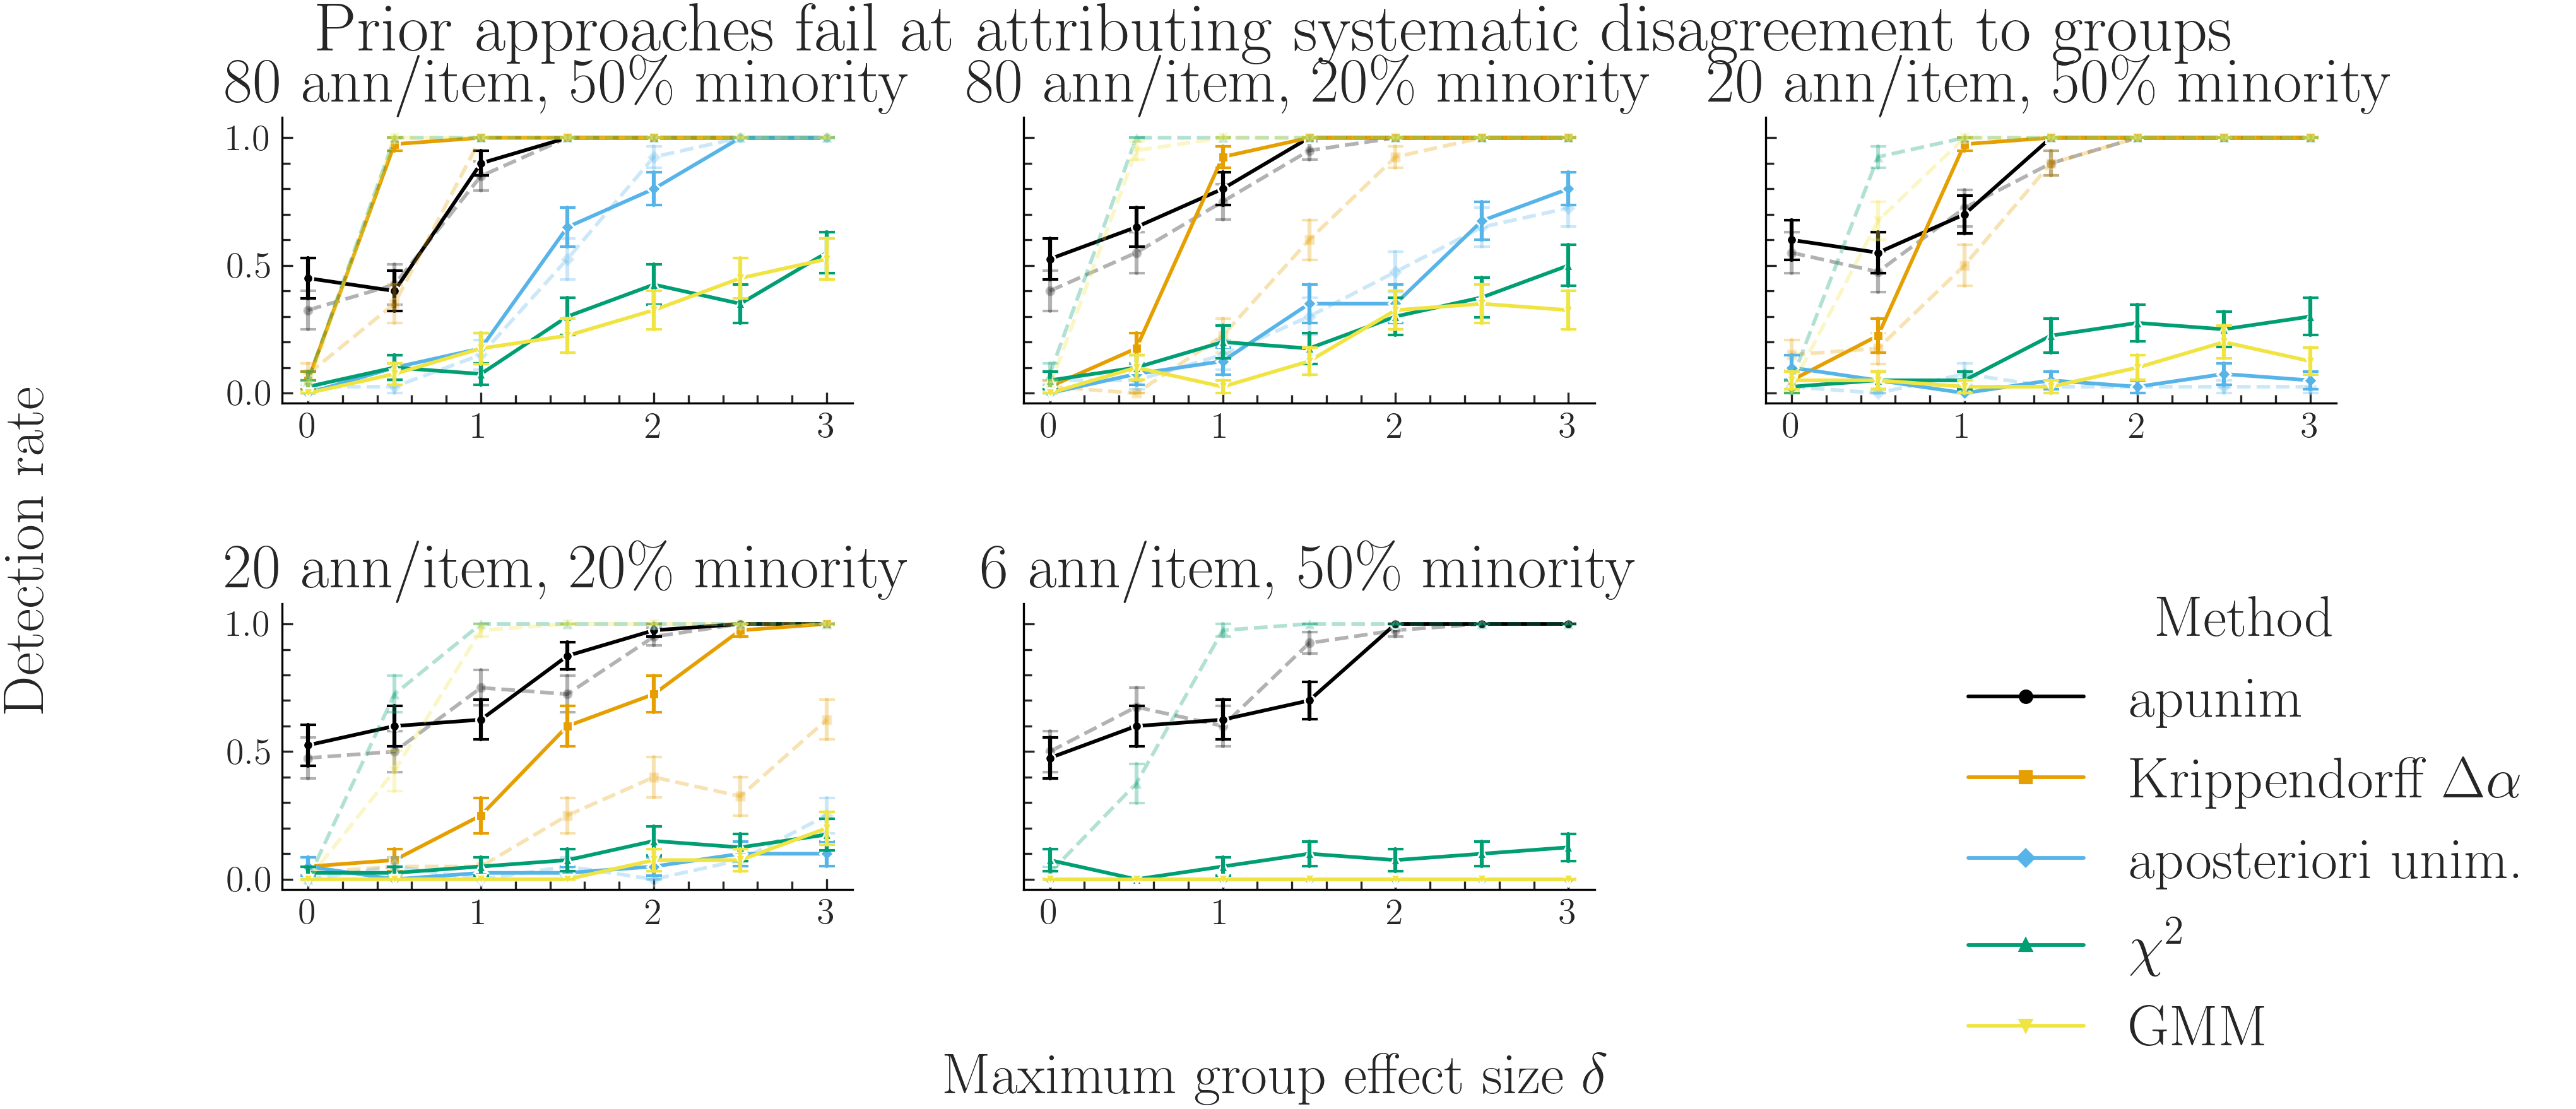
\includegraphics[width=\linewidth]{metric_comparison.png}
	\caption{\ac{sysdis} attribution on synthetic distributions. When \ac{sysdis} exists, the mean of the normal distributions shifts according to the value of the x-axis. The y-axis shows the accuracy of each method when attempting to recover the (known) \ac{sdd} causing polarization. Bars indicate standard error. Dashed lines show the results of a simplified experimental setup, where disagreement always has the same direction.}
	\label{fig:measures}
\end{figure}

\paragraph{Experimental Setup} We compare the effectiveness of our method (introduced in \S\ref{sec:apunim}), the \ac{au} framework proposed by \citet{pavlopoulos-likas-2024}, the $\chi^2$ method presented in \citet{akhtar_2019}, GMM clustering used in \citet{checco_2017}, and a baseline using \ac{iaa} ($\Delta \alpha$ Krippendorff) on simulated distributions (App.~\ref{app:experiments} for details and assumptions). To determine whether a score is statistically significant, we construct a null distribution for each method with the null hypothesis that the group labels are unrelated to the observed annotations. We therefore repeatedly shuffle the labels across annotators, recompute the method's statistic, and use the resulting scores to form the null distribution. Since we construct the distributions, we have knowledge of the \emph{ground-truth} for which \ac{sdd} is causing polarization (which is not the case for real-life or LLM annotations), which we can inject to test whether it is retrieved by each method.

\paragraph{Conditions} Annotations are generated according to $y_{ij} = b_j + g_i p_j + \epsilon_{ij}$,  where $b_j$ is the baseline rating for item $j$, $g_i \in \{-\frac{1}{2}, +\frac{1}{2}\}$ indicates the annotator's group, $p_j$ controls the magnitude and direction of \ac{sysdis} for item $j$, and $\epsilon_{ij}$ is annotation noise. We use two simulation setups that differ only in how $p_j$ is defined:
\begin{enumerate*}
	\item \textbf{Unidirectional}: $p_j \sim \text{Uniform}(0, \delta)$. The group effect always favors the same group across all items, though its magnitude varies per item.
	
	\item \textbf{Bidirectional}: $p_j \sim \text{Uniform}(-\delta, +\delta)$. The direction of the group effect can vary across items, so that groups may systematically disagree in opposite directions on different items.
\end{enumerate*}

\paragraph{Results} As shown in Fig.~\ref{fig:measures}, \emph{both the $\chi^2$ and GMM methods generally fail} at attributing \ac{sysdis} to any group. \ac{iaa} remains usable when many annotators are available, but underperforms in cases where the examined group is a minority and when a few annotators are available per item (a common case among \ac{nlp} datasets---see \S\ref{sec:datasets}).\footnote{While this figure explores a case with only two groups, ablations with $k=\{3,5,10\}$ groups per \ac{sdd} can be found in App.~\ref{app:ablation}; Fig.~\ref{fig:measures-multiple}.}


\subsection{On Real Data}

\begin{table*}
	\caption{Statistical significance of each \ac{pc} feature per method. \sigyes: significant at $p<0.05$ after Bonferroni correction across the features of the dataset; \signo: not significant. The method \textit{am} refers to our method, ``apunim''.}
	\label{tab:real-data-methods}
	\centering
	\scriptsize
	\begin{tabular}{l*{27}{c}}
		\toprule
		& \multicolumn{4}{c}{DICES-350} & \multicolumn{4}{c}{DICES-990} & \multicolumn{3}{c}{Sap et al. 2022} & \multicolumn{11}{c}{Kumar et al. 2021} & \multicolumn{5}{c}{POPQUORN} \\
		\cmidrule(lr){2-5} \cmidrule(lr){6-9} \cmidrule(lr){10-12} \cmidrule(lr){13-23} \cmidrule(lr){24-28}
		\rotatebox{90}{\textbf{Method}} 
		& \rotatebox{90}{Age} & \rotatebox{90}{Education} & \rotatebox{90}{Gender} & \rotatebox{90}{Race}
		& \rotatebox{90}{Age} & \rotatebox{90}{Education} & \rotatebox{90}{Gender} & \rotatebox{90}{Race}
		& \rotatebox{90}{Age} & \rotatebox{90}{Ethnicity} & \rotatebox{90}{Gender}
		& \rotatebox{90}{Age} & \rotatebox{90}{Education} & \rotatebox{90}{Ethnicity} & \rotatebox{90}{Gender/Trans} & \rotatebox{90}{Targeted} & \rotatebox{90}{Parent} & \rotatebox{90}{Politics} & \rotatebox{90}{Religion} & \rotatebox{90}{Tox.Seen/Problem} & \rotatebox{90}{Sex. Orient.} & \rotatebox{90}{Tech Impact}
		& \rotatebox{90}{Age} & \rotatebox{90}{Education} & \rotatebox{90}{Gender} & \rotatebox{90}{Occupation} & \rotatebox{90}{Race} \\
		\midrule
		am
		& \signo & \sigyes & \signo & \sigyes
		& \sigyes & \sigyes & \sigyes & \sigyes
		& \signo & \signo & \sigyes
		& \signo & \signo & \signo & \signo & \signo & \signo & \signo & \signo & \signo & \signo & \signo
		& \signo & \sigyes & \signo & \signo & \sigyes \\
		$\Delta\alpha$
		& \signo & \signo & \sigyes & \sigyes
		& \signo & \sigyes & \sigyes & \signo
		& \signo & \signo & \sigyes
		& \signo & \signo & \signo & \signo & \signo & \signo & \signo & \signo & \signo & \signo & \signo
		& \signo & \signo & \signo & \signo & \signo \\
		\ac{au}
		& \signo & \signo & \signo & \signo
		& \signo & \signo & \signo & \signo
		& \signo & \signo & \signo
		& \signo & \signo & \signo & \signo & \signo & \signo & \signo & \signo & \signo & \signo & \signo
		& \signo & \signo & \signo & \signo & \signo \\
		$\chi^2$
		& \sigyes & \sigyes & \sigyes & \sigyes
		& \sigyes & \sigyes & \sigyes & \sigyes
		& \sigyes & \sigyes & \sigyes
		& \sigyes & \sigyes & \sigyes & \sigyes & \sigyes & \sigyes & \sigyes & \sigyes & \sigyes & \sigyes & \sigyes
		& \sigyes & \sigyes & \sigyes & \sigyes & \sigyes \\
		\bottomrule
	\end{tabular}
\end{table*}

Table~\ref{tab:real-data-methods} shows a comparison between the different methods when applied to the five datasets introduced in \S\ref{sec:datasets}. The GMM method is not run, as it requires the exact same annotators to annotate the items in each dataset, which is not the case for any of our datasets. This limitation makes the test extremely restrictive in realistic annotation settings. We explain our own method in \S\ref{sec:apunim}, as the focus of this experiment is the behavior of other measures on real data.

We find that the \ac{au} method completely fails to attribute polarization to any \ac{sdd}, while the $\chi^2$ method attributes it to every single one. The latter can be explained by the assumptions made by the test; namely that annotations can be pooled across items (discussed in the next section), as well as the power of the test which inflates p-values when the number of observations is large enough. Out of all prior methodologies, \ac{iaa} using Krippendorff's $\alpha$ seems to be the only way of obtaining any results for only a subset of datasets.


\subsection{The Issue of Inter-Item Annotation Aggregation}

\begin{figure}[t]
	\centering
	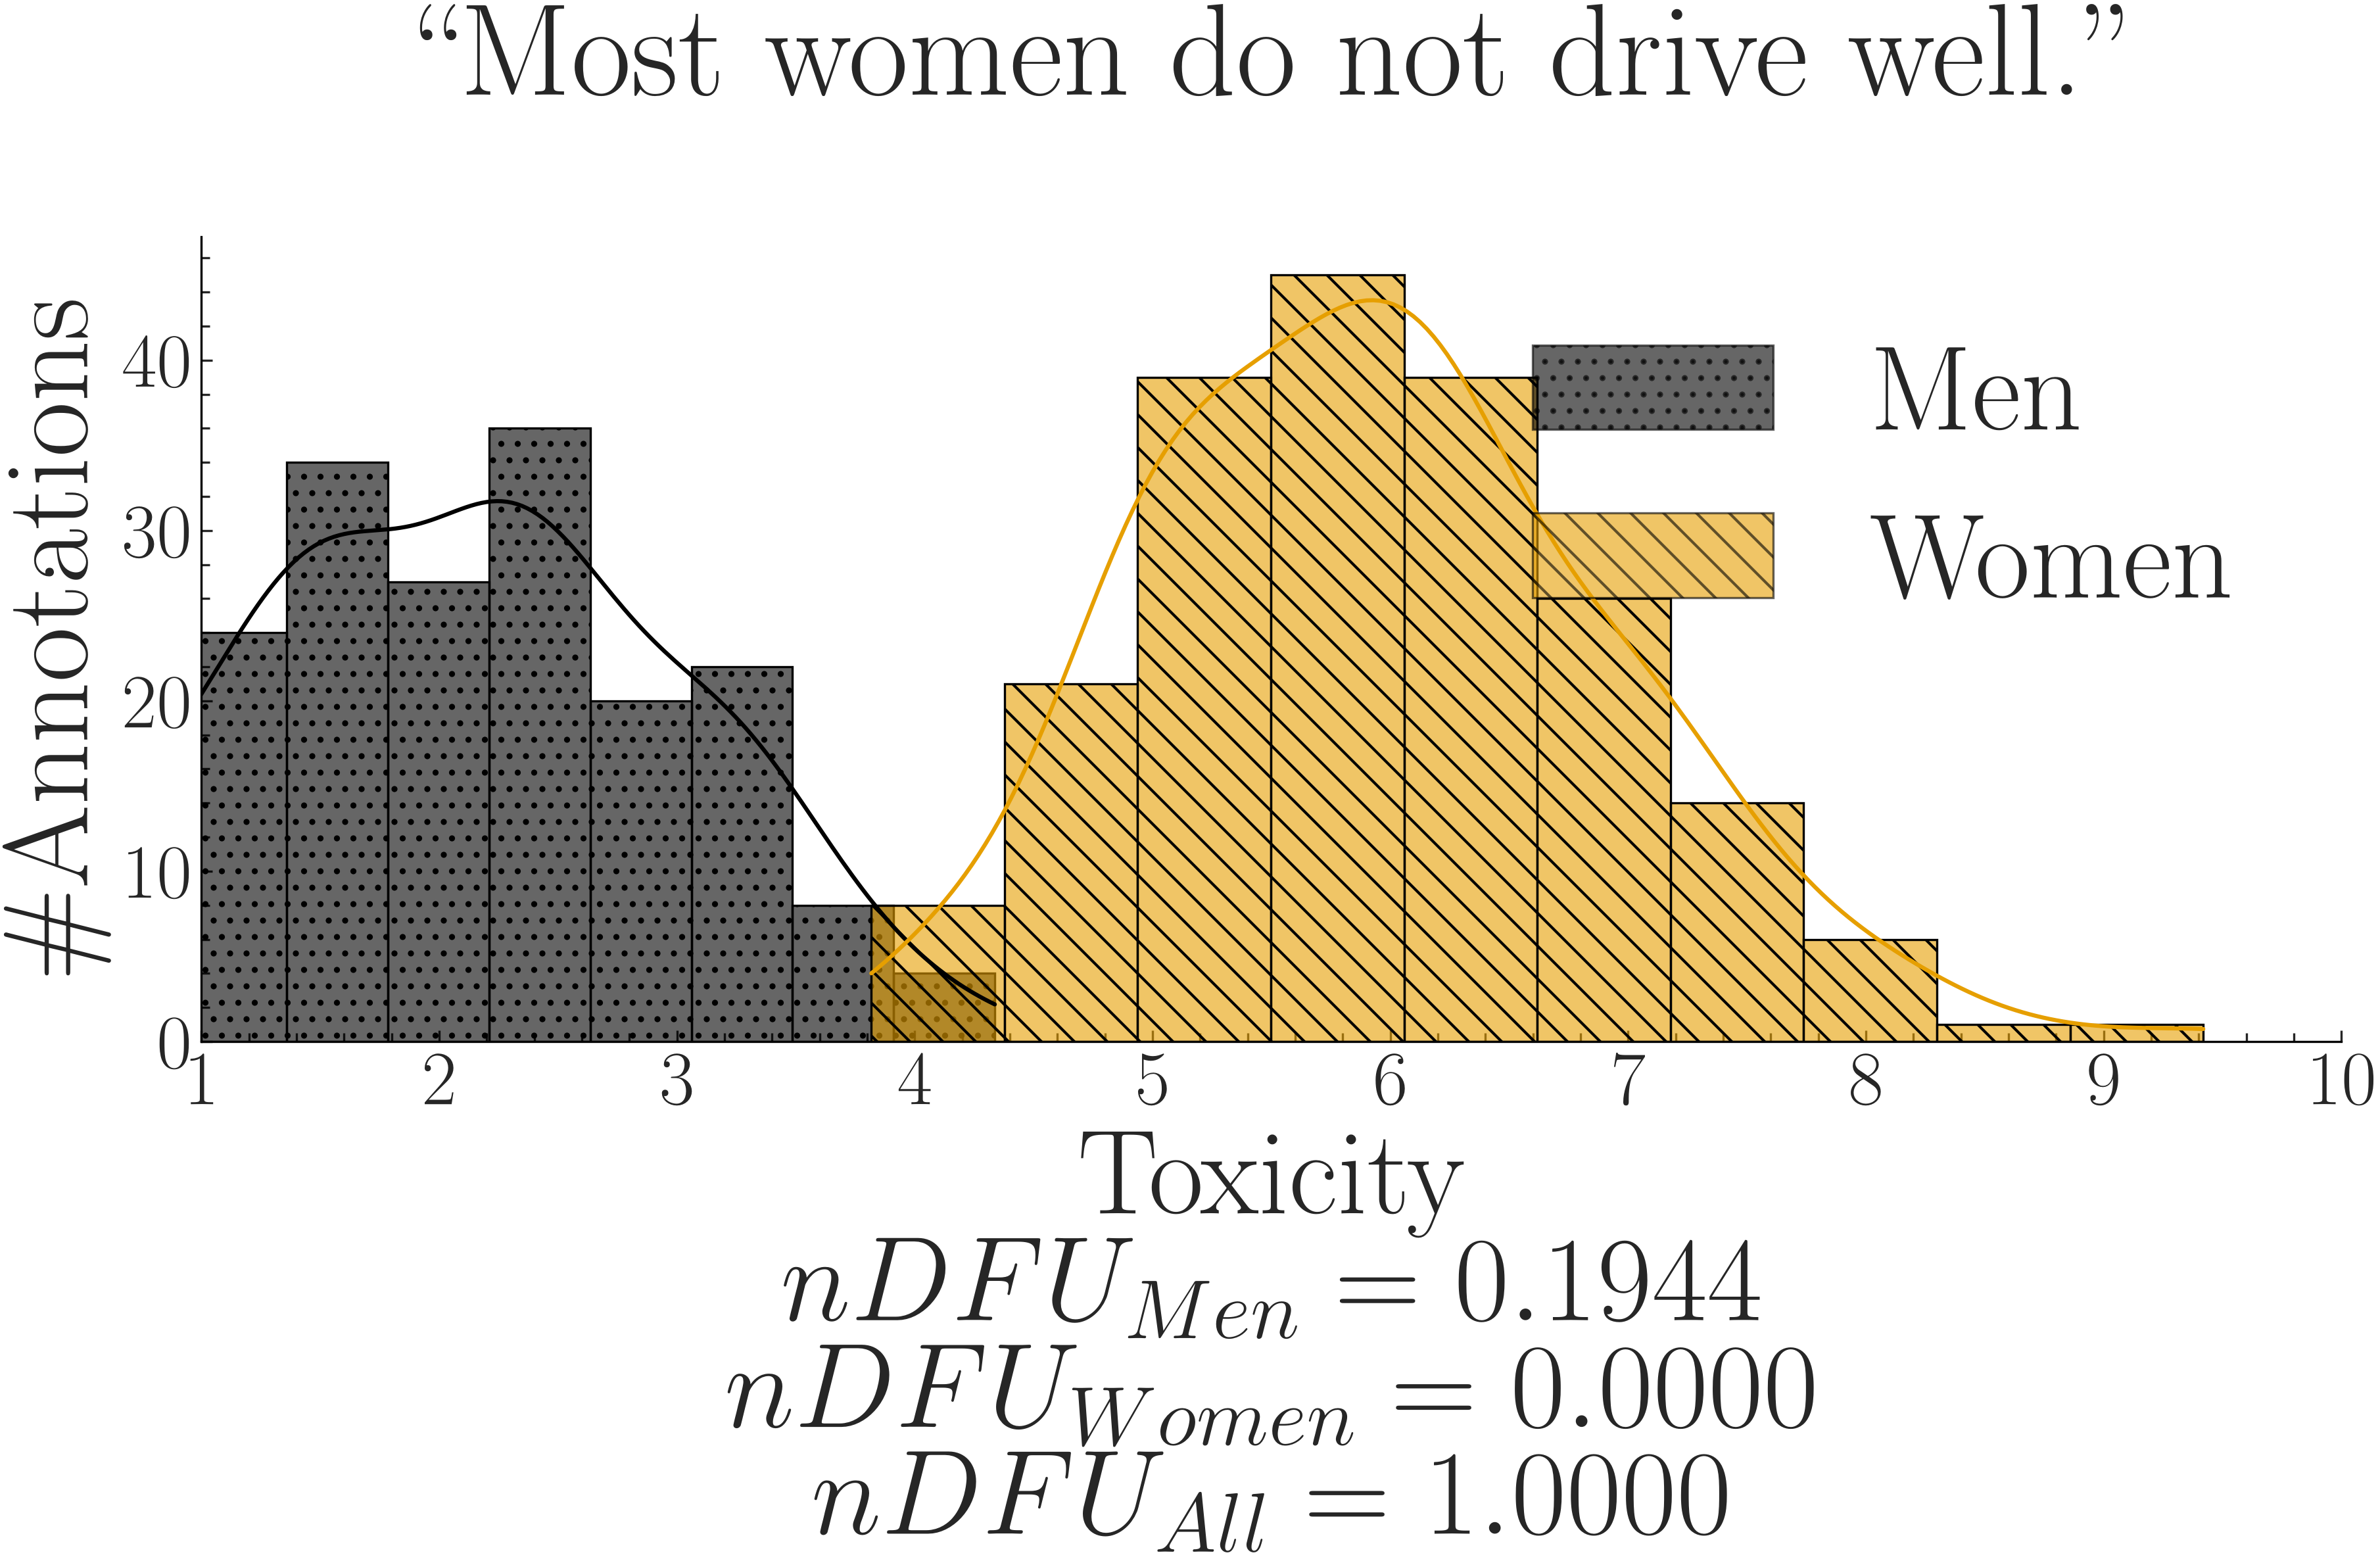
\includegraphics[width=0.32\linewidth]{ndfu_comment1.png}
	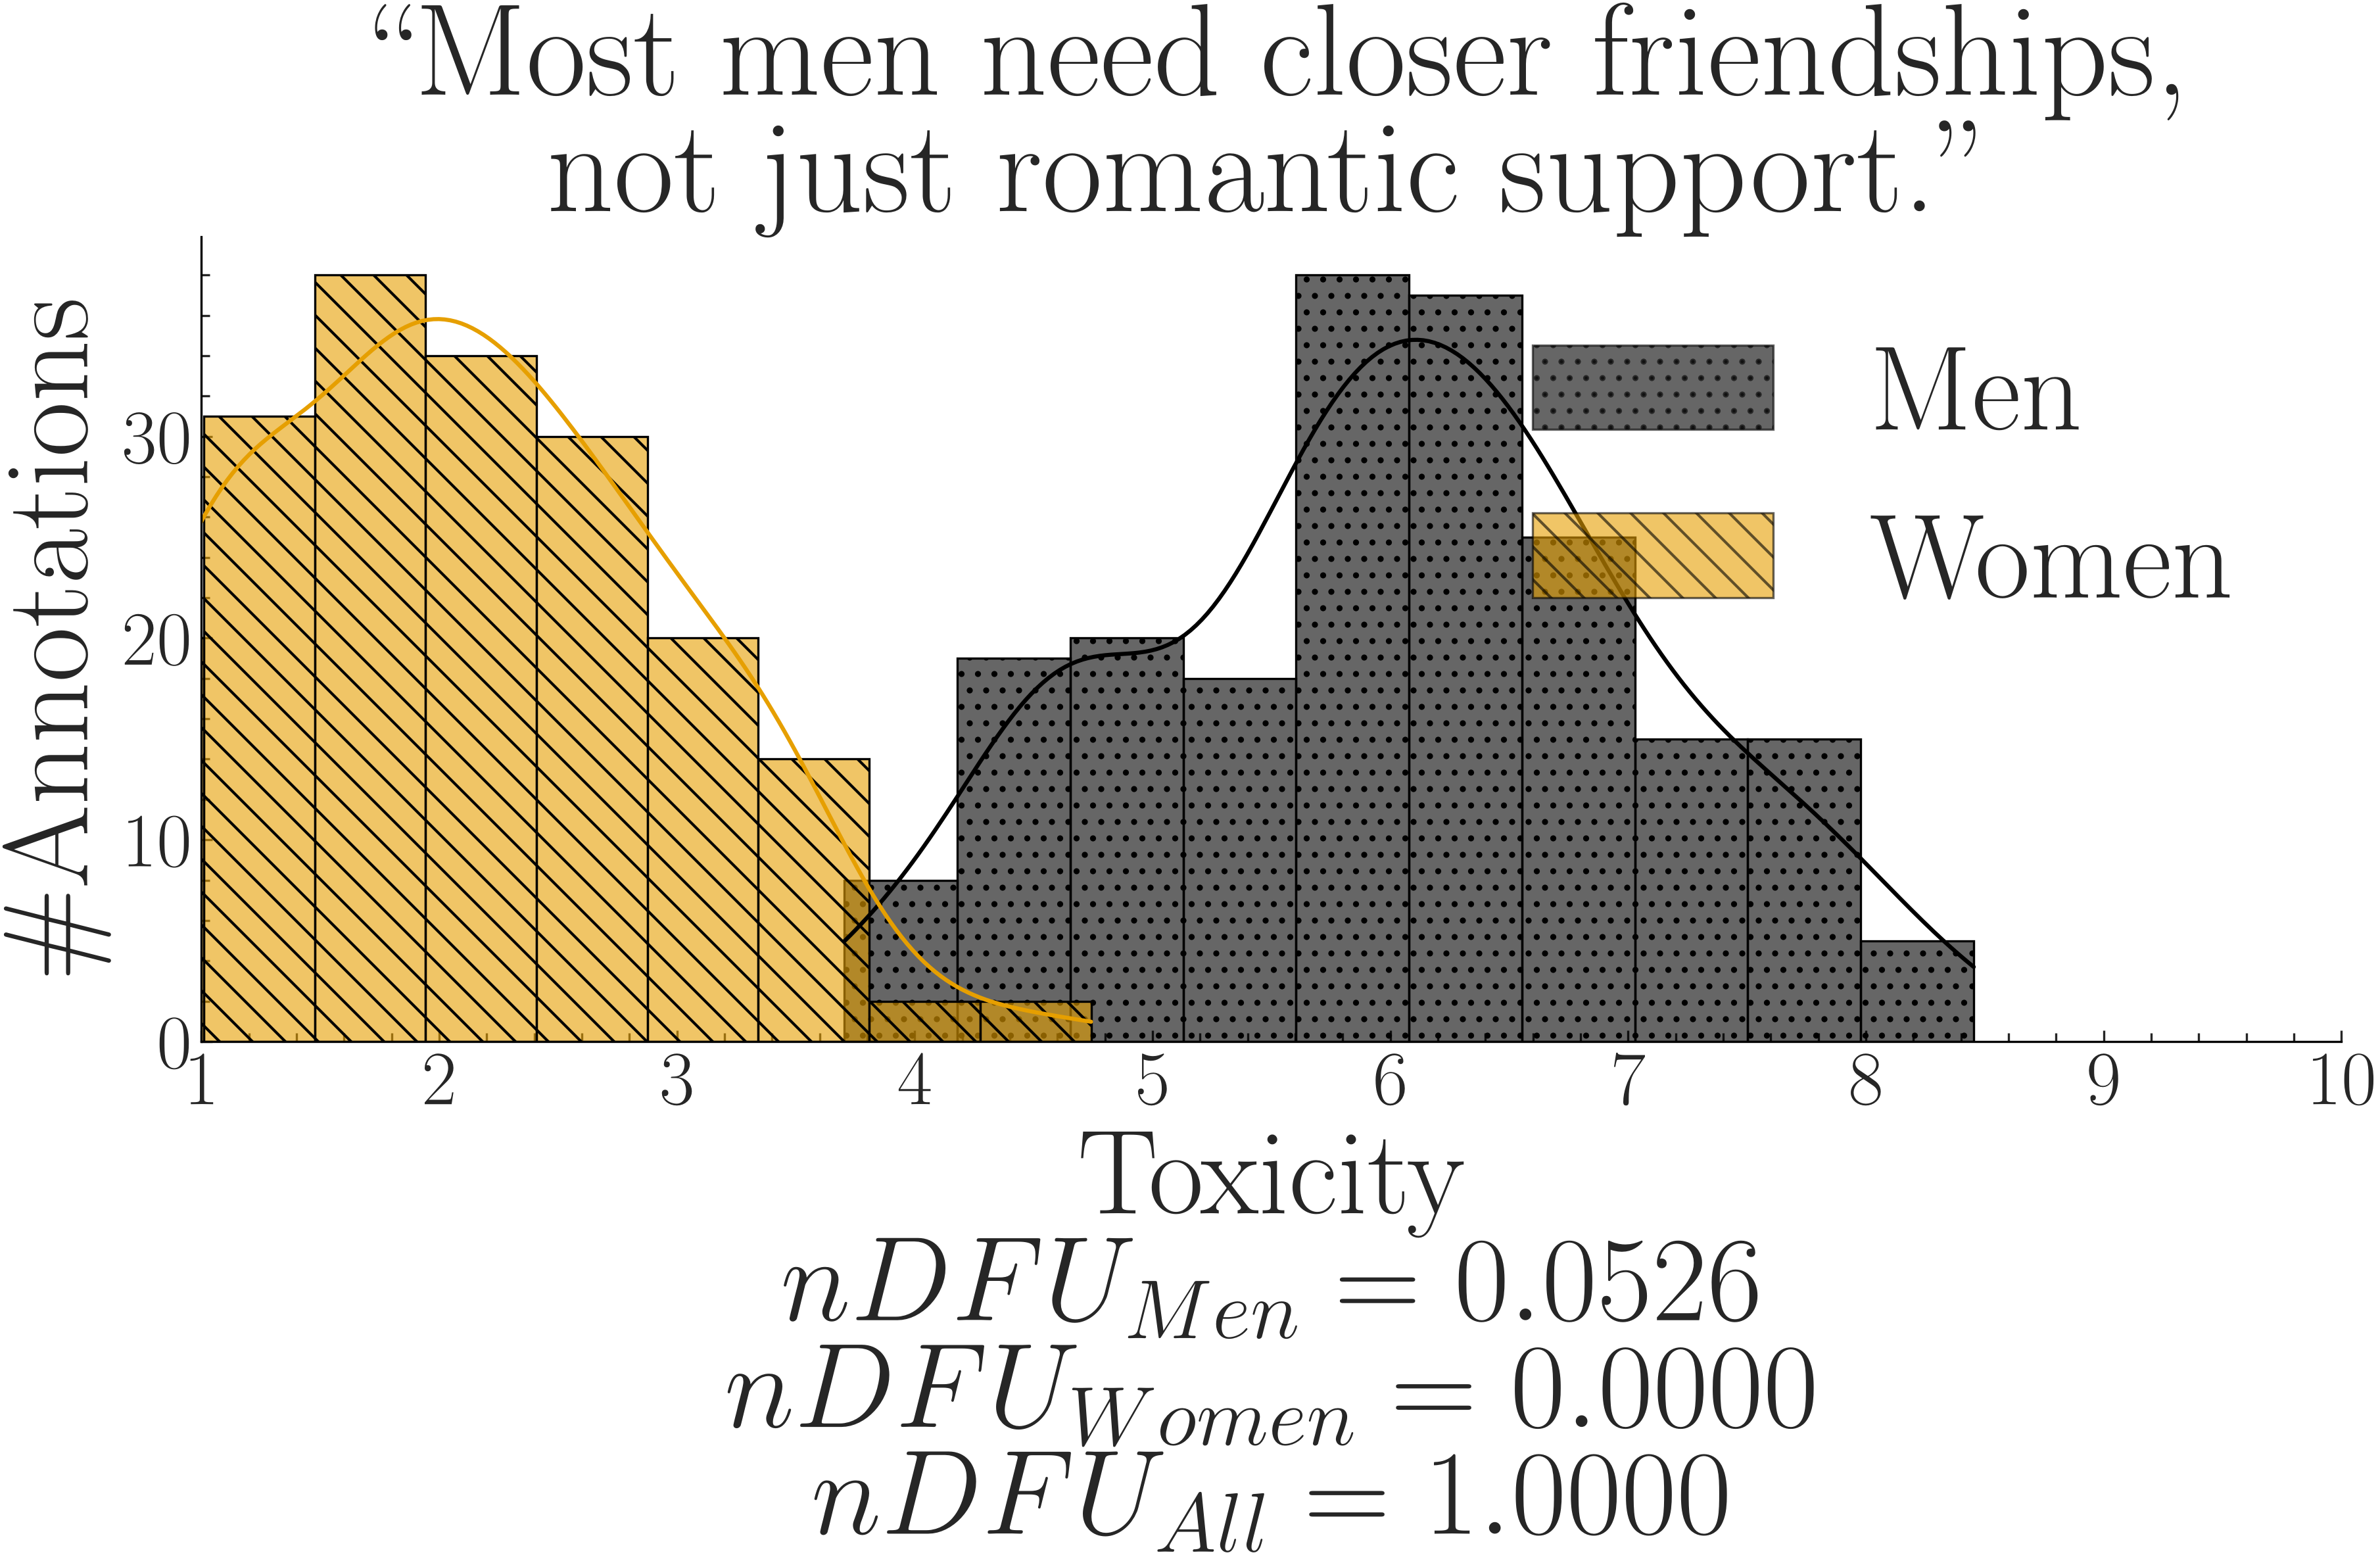
\includegraphics[width=0.32\linewidth]{ndfu_comment2.png}
	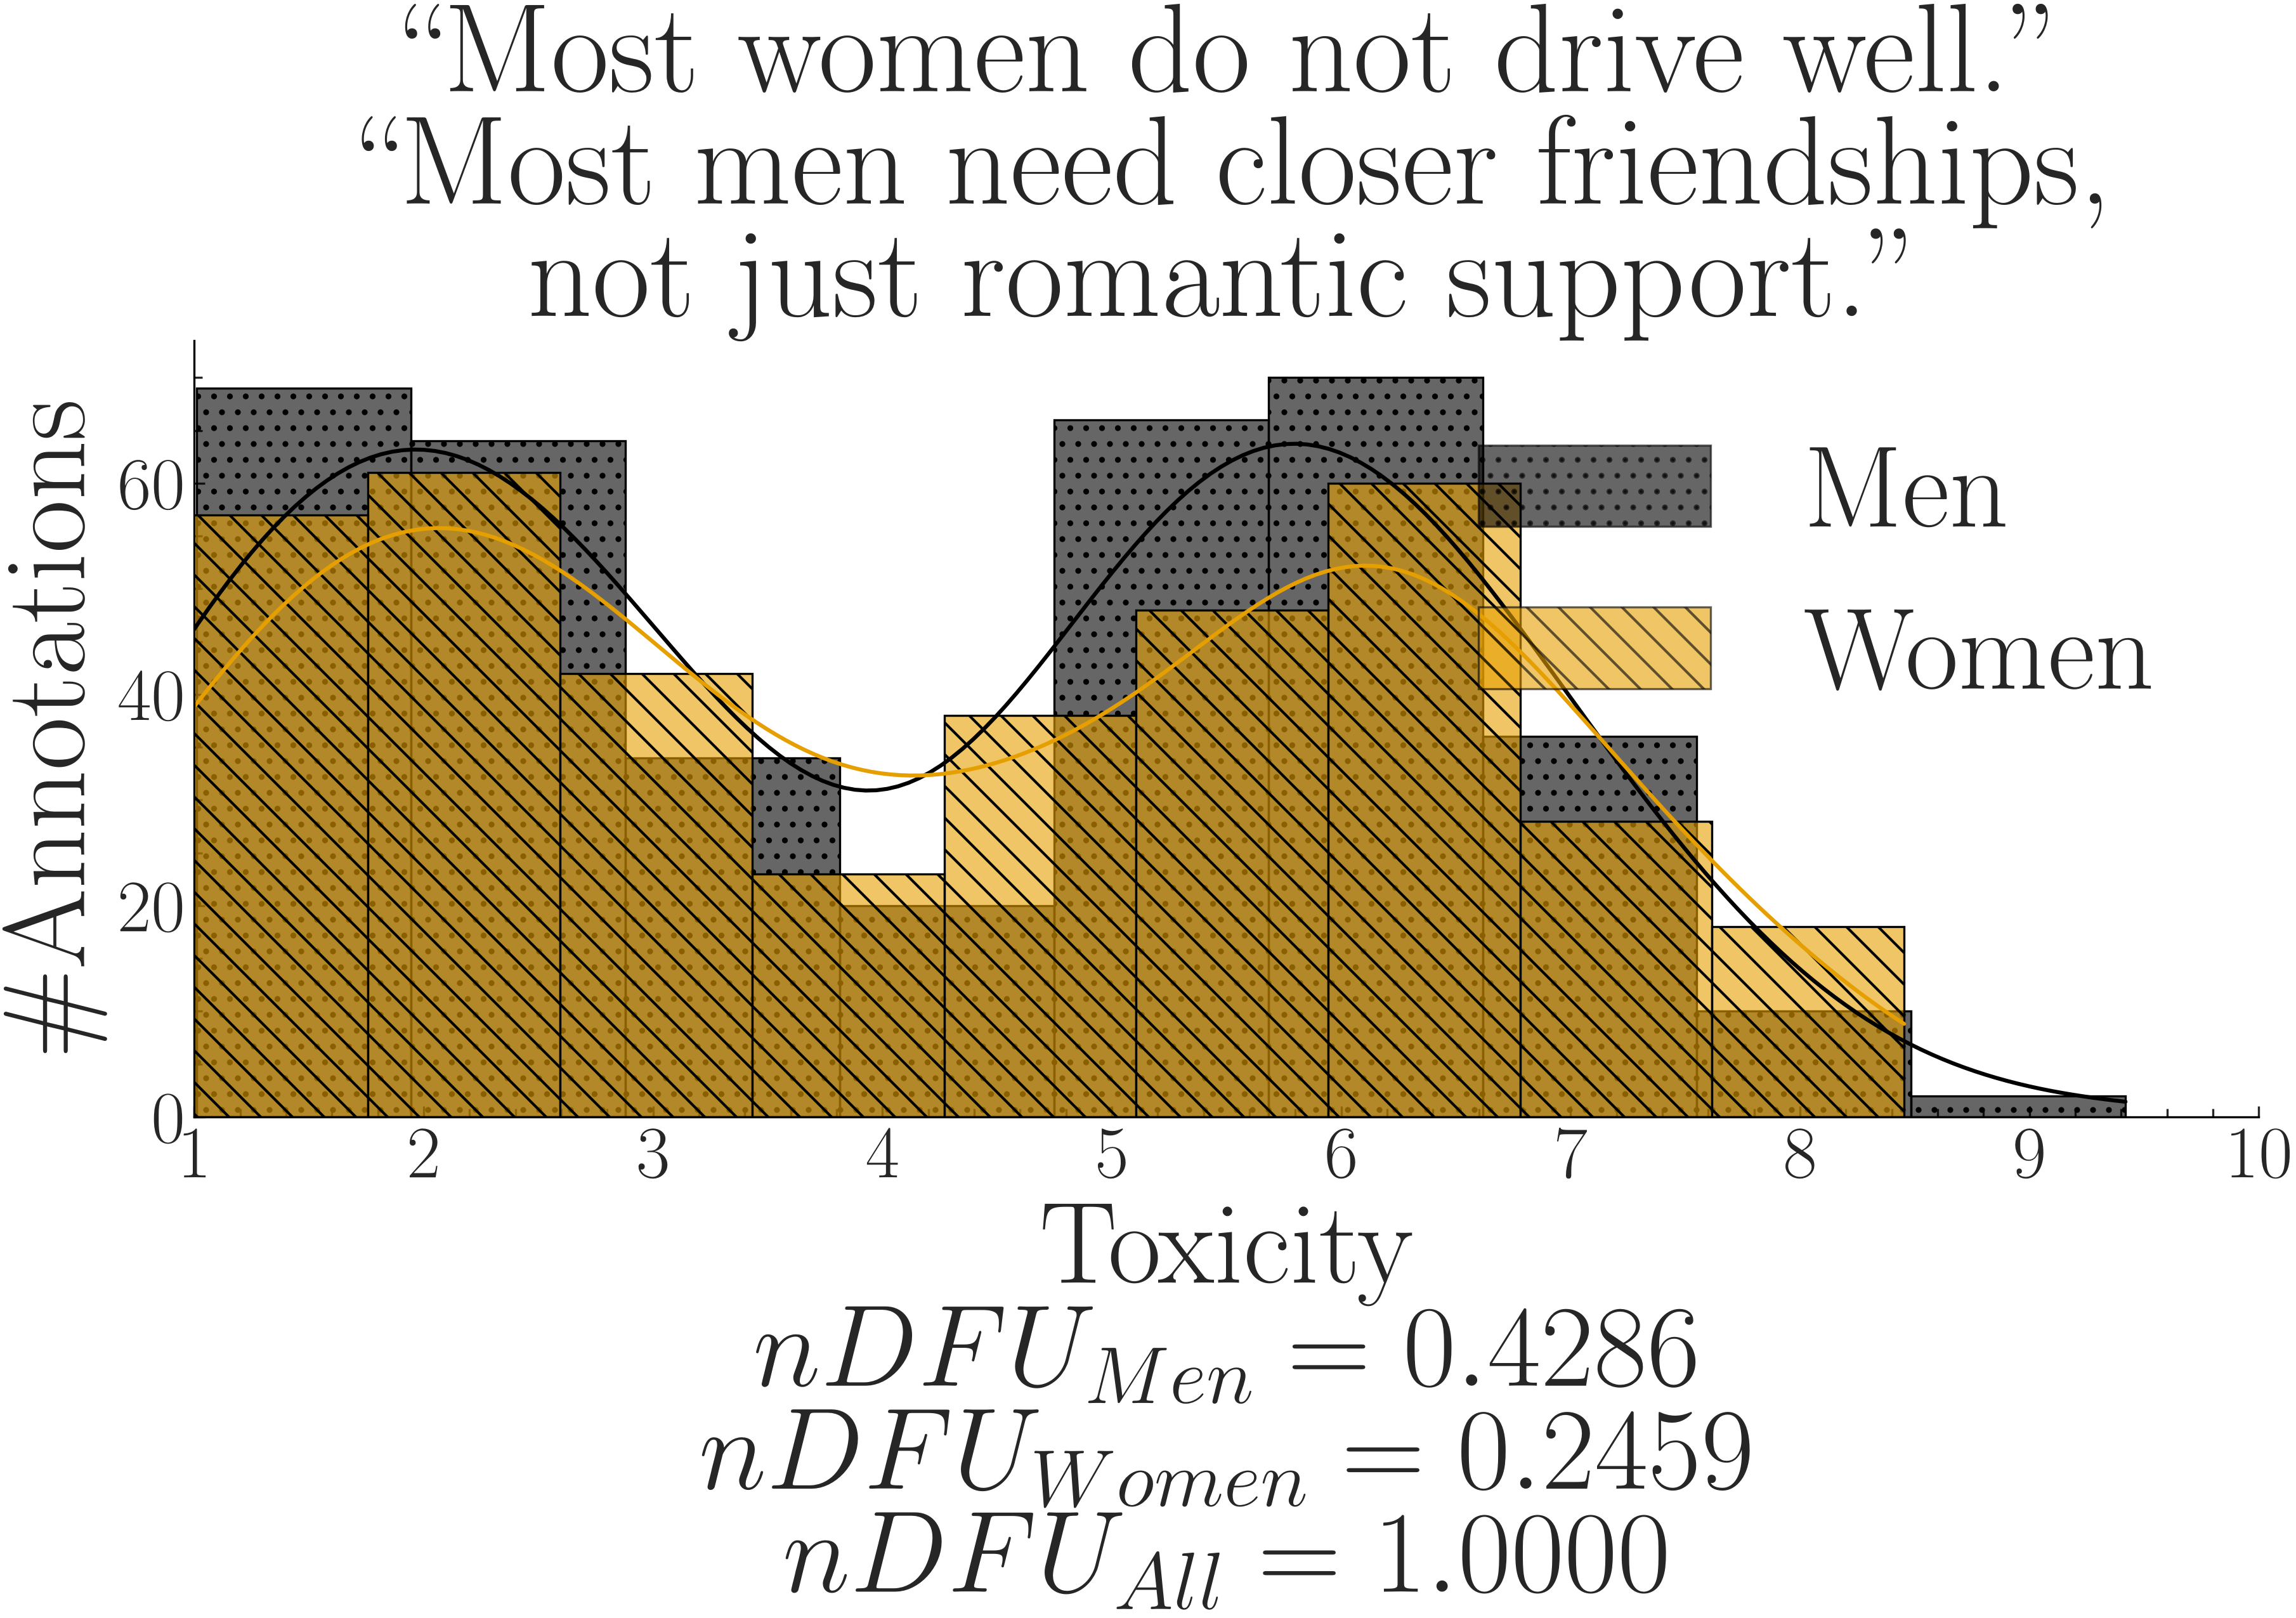
\includegraphics[width=0.32\linewidth]{ndfu_discussion.png}
	\caption{Synthetic experiment showing two comments with annotators disagreeing about which one is toxic. Instead of comparing two unimodal distributions (comments viewed separately) with two bimodal distributions (their aggregated annotations), we end up comparing two bimodal distributions during aggregation, obscuring the source of the polarization (explained by gender, but not shown).}
	\label{fig:ndfu_discussion}
\end{figure}

In Fig.~\ref{fig:measures} we observed that the simple statistical approaches show excellent performance when all groups are polarized in the same way. This is expected, since their assumption of a consistent, fixed means effects, is violated in the second experimental setup. Specifically, both $\chi^2$ and GMM aggregate across items before looking for group differences; $\chi^2$ pools all annotations into a single contingency table, while GMM clusters annotators by their mean rating across items. In both cases, opposite-direction effects (see Fig.~\ref{fig:ndfu_discussion}) cancel out in the aggregate, making the two groups appear statistically indistinguishable. We can confirm the persistence of this issue using \ac{ndfu} \citep{pavlopoulos-likas-2024}, which is another representation of polarization (Eq.~\ref{eq:ndfu}) in Fig.~\ref{fig:ndfu_discussion}, which shows that two items polarized for the opposite reason may lead to a false negative. We avoid this issue in \S\ref{sec:apunim} by computing annotation statistics item-by-item.

\begin{finding}
	\label{finding:methods}
	Current methodologies attributing \ac{sysdis} generally fail in realistic annotation conditions. One of the reasons is that disagreements may conflict across items, which may compromise cross-item annotation aggregation.
\end{finding}


\section{Comparing Human and LLM Polarization}
\label{sec:apunim}

\subsection{Quantifying Attribution to Annotator Dimensions}

We estimate polarization using \ac{ndfu} (see \S\ref{sec:related}; Eq.~\ref{eq:apunim}). Specifically, we measure the unimodality of each group $g$ for an item $c$ as $Pol_g(c) = \textit{nDFU}(A_g(c))$, where $A_g(c)$ is the set of annotations for item $c$ created by annotators belonging to a group $g$. We compare this quantity to the ``apriori'' polarization present in the item c, which is defined as the \emph{expected} (average) unimodality of theoretical groups $\mathrm{Pol}_{\textit{apr}}(c) = \frac{1}{k} \sum_{1}^{k}  \mathrm{nDFU}(A_{random}(c))$, where $A_{random}$ is a random split and $k$ is a hyperparameter (higher $k$ yields more accurate estimation, at a greater computational cost). Intuitively, a high $\mathrm{Pol}_{\textit{apr}}(c)$ score means that much of the polarization is likely not driven by any single group. 

Since the  $\mathrm{Pol}_{\textit{apr}}(c)$ and $Pol_g(c)$ quantities represent very noisy estimates due to the lack of annotators per item, a direct comparison would not be reliable. We therefore exploit the Law of Large Numbers to compute the statistic on the dataset level and average both quantities for all items in the dataset $D$. Normalizing this difference yields the measure described in Eq.~\ref{eq:ndfu}, which we call \emph{apunim}:

\begin{equation}
	\label{eq:apunim}
	\textit{apunim}(D, g) = \frac{\mathbb{E}_{c \in D} \left[ \mathrm{Pol}_{\textit{apr}}(c) \right] - \mathbb{E}_{c \in D} \left[ Pol_g(c)\right] }{1 - \mathbb{E}_{c \in D} \left[ \mathrm{Pol}_{\textit{apr}}(c) \right]}
\end{equation}

The \emph{sign} of apunim carries information agreement-based attribution does not:

\begin{itemize}
	\item$\textit{apunim}(g) \approx 0$: The group $g$ does not meaningfully disagree with the other annotators.
	\item $\textit{apunim}(g) > 0$: The group $g$ has fundamental disagreements with the other annotators. 
	\item $\textit{apunim}(g) < 0$: The annotators of group $g$ are polarized between themselves.
\end{itemize}

Apunim thus measures the degree to which an annotator group contributes to overall polarization in a set of items. As demonstrated in \S\ref{sec:methods}; Fig.~\ref{fig:measures}, our measure is robust to the number of annotators per item, opposing \ac{sysdis} effects, and minority groups, validating our initial motivation. Furthermore, unlike some prior methods \citep{akhtar_2019, checco_2017}, apunim allows us to attribute \ac{sysdis} to a specific group, not just a \ac{sdd} (e.g., only ``men'' instead of ``gender'' as a whole), allowing fine-grained analysis. We include a perturbation-based p-value estimation, which tests whether the observed apunim value of a group $g$ statistically surpasses that of random groups in App.~\ref{app:pvalue} and analyze theoretical design decisions, limitations and computational details in App.~\ref{app:design}.


\subsection{How Are Humans Polarized?}

\begin{table}[t]
	\caption{Statistically significant ($p<0.05$) apunim results across the Sap and DICES datasets. Gray rows show \texttt{Ethnicity} and \texttt{Gender} groups. ``Support'' refers to number of annotations. Consult App.~\ref{app:full} for the full results.}
	\label{tab:apunim-main}
	\small
	\centering
	\setlength{\tabcolsep}{4pt}
	\begin{minipage}[t]{0.485\linewidth}
		\begin{tabularx}{\linewidth}{X r r}
			\toprule
			\textbf{Group} & \textbf{Apunim} & \textbf{Support} \\
			\midrule
			\multicolumn{3}{c}{\textbf{DICES-990}} \\
			\midrule
			\rowcolor{gray!15}
			Ethnicity=AfricanAm & 0.0995 & 5148 \\
			\rowcolor{gray!15}
			Ethnicity=Latino & -0.0631 & 5877 \\
			\rowcolor{gray!15}
			Ethnicity=Other & 0.0340 & 21669 \\
			\rowcolor{gray!15}
			Ethnicity=White & -0.0649 & 10166 \\
			\rowcolor{gray!15}
			Gender=Man & 0.0359 & 28817 \\
			\rowcolor{gray!15}
			Gender=Woman & -0.0271 & 29990 \\
			Age=GenZ & 0.0469 & 12214 \\
			Age=Millennial & -0.0068 & 34433 \\
			Age=GenX+ & -0.0282 & 12699 \\
			Education=College & 0.0063 & 52727 \\
			Education=High school & -0.0500 & 6619 \\
			\bottomrule
		\end{tabularx}
	\end{minipage}
	\hfill
	\begin{minipage}[t]{0.485\linewidth}
		\begin{tabularx}{\linewidth}{X r r}
			\toprule
			\textbf{Group} & \textbf{Apunim} & \textbf{Support} \\
			\midrule
			\multicolumn{3}{c}{\textbf{DICES-350}} \\
			\midrule
			\rowcolor{gray!15}
			Ethnicity=AfricanAm & -0.0366 & 7627 \\
			\rowcolor{gray!15}
			Ethnicity=Asian & 0.0445 & 6838 \\
			Education=Other & -0.0230 & 1841 \\
			\midrule
			\multicolumn{3}{c}{\textbf{Sap}} \\
			\midrule
			\rowcolor{gray!15}
			Gender=Man & -0.1508 & 1254 \\
			\rowcolor{gray!15}
			Gender=Woman & 0.2613 & 693 \\
			Age=GenX+ & -0.1670 & 223 \\
			\midrule
			\multicolumn{3}{c}{\textbf{POPQUORN}} \\
			\midrule
			\rowcolor{gray!15}
			Gender=Man & 0.0081 & 2720 \\
			\rowcolor{gray!15}
			Race=Black & -0.1572 & 222 \\
			Education=College & 0.0496 & 2388 \\
			Education=Graduate & -0.0808 & 468 \\
			\bottomrule
		\end{tabularx}
	\end{minipage}
\end{table}

\paragraph{Experimental Setup} Assuming a confidence level of $\alpha=0.05$ we test whether any of the provided \acp{sdd} can explain the \ac{sysdis} shown in the five datasets (\S\ref{sec:datasets}). Statistically significant results are presented in Table~\ref{tab:apunim-main}.\footnote{The results are not necessarily contingent on a reliable p-value estimation, as non-statistically significant results have very low ($<0.01$) apunim values. A threshold on the apunim values would produce similar tables.} Note that our analysis is necessarily uni-dimensional due to the lack of annotation meta-data. App.~\ref{app:ablation}; Fig.~\ref{fig:std_error} shows that our results are \emph{robust to small annotator counts}, corroborating the synthetic experiments in Fig.~\ref{fig:measures}. See App.~\ref{app:software} for details on parameters and execution times and App.~\ref{app:full} for the full results.

\paragraph{Results} \emph{\ac{sysdis} is consistently attributed to \textbf{ethnicity}} across all datasets excluding DICES-330, confirming prior work suggesting that it is a systematic source of annotator disagreement in \ac{hs} tasks~\citep{goyal2022your}. Additionally, in both DICES-990, Sap and POPQUORN, \ac{sysdis} is attributed to \textbf{gender}, which is consistent with previous findings~\citep{wojatzki2018women, binns2017like}. None of the \acp{sdd} in the Kumar dataset show statistically significant values, but this is expected, since our methodology requires at least six annotators per item to work reliably.\footnote{Note that \acp{aa} show differently signed apunim values in the two DICES datasets, which may be attributed to these datasets using different labels (see \S\ref{sec:datasets}) and because different ethnic group splits are considered in each dataset. Thus, while detection is constant across the two datasets, attribution is not. Additionally, men are a consistent source of \ac{sysdis} (positive values), while women disagree among themselves (positive values) in DICES-990 and POPQUORN, but the opposite is true for Sap. Unfortunately we can not diagnose these discrepancies, since neither DICES nor Sap include annotation guidelines (Table~\ref{tab:datasets}).}

\begin{finding}
	\label{finding:human}
	Ethnicity and gender are consistent causes of \ac{sysdis}, confirming prior literature on Toxicity and \ac{hs} tasks.
\end{finding}


\subsection{How Are LLMs Polarized?}
\label{sec:llms}
%TODO: Gemma31b kumar
\begin{table}[t]
\small
\centering
\caption{Mean (SE) per-comment \ac{ndfu} of the human annotations
        and of the LLM annotations under the default prompt, per dataset
        and pooled over all datasets (All). $n$ is the number of
        comments. Excluding the following models: llama8b, olmo7b, qwen7b.}
\label{tab:mean-ndfu-default-vs-human-excluding}
\begin{tabular}{lrrrrrrrr}
\toprule
 & \multicolumn{2}{c}{Sap et al. 2022} & \multicolumn{2}{c}{Kumar et al. 2021} & \multicolumn{2}{c}{POPQUORN} & \multicolumn{2}{c}{All} \\
 & n & Mean (SE) & n & Mean (SE) & n & Mean (SE) & n & Mean (SE) \\
Model &  &  &  &  &  &  &  &  \\
\midrule
Human & 585 & 0.38 (0.01) & 1000 & 0.42 (0.01) & 1500 & 0.31 (0.01) & 3085 & 0.36 (0.00) \\
olmo32b & 585 & 0.24 (0.01) & 1000 & 0.51 (0.01) & 1500 & 0.46 (0.01) & 3085 & 0.43 (0.01) \\
qwen32b & 585 & 0.18 (0.01) & 1000 & 0.19 (0.01) & 1500 & 0.25 (0.01) & 3085 & 0.22 (0.01) \\
mistral7b & 585 & 0.21 (0.01) & 1000 & 0.37 (0.01) & 1500 & 0.40 (0.01) & 3085 & 0.35 (0.01) \\
mistral24b & 585 & 0.25 (0.01) & 1000 & 0.25 (0.01) & 1500 & 0.33 (0.01) & 3085 & 0.29 (0.00) \\
gemma7b & 585 & 0.19 (0.01) & 1000 & 0.22 (0.01) & 1500 & 0.15 (0.01) & 3085 & 0.18 (0.00) \\
gemma31b & 585 & 0.04 (0.01) & 1000 & 0.09 (0.01) & --- & --- & 1585 & 0.07 (0.00) \\
\bottomrule
\end{tabular}
\end{table}

\begin{table}[t]
\caption{Cohen's d between the default and each adversarial
        instruction prompt, computed on the per-comment \ac{ndfu}. Results
        are given per model, for each dataset separately and as the
        unweighted mean over datasets (All). Comments per model: Sap et al. 2022: 585; Kumar et al. 2021: 1000; POPQUORN: 1500 (gemma31b: 0). Excluding the following models: llama8b, olmo7b, qwen7b.}
\label{tab:cohens-d-excluding}
\centering
\footnotesize
\setlength{\tabcolsep}{1.5pt}
\begin{tabular}{l rrrr@{\hspace{4pt}}rrrr@{\hspace{4pt}}rrrr@{\hspace{4pt}}rrrr}
\toprule
 & \multicolumn{4}{c}{All} & \multicolumn{4}{c}{Sap et al. 2022} & \multicolumn{4}{c}{Kumar et al. 2021} & \multicolumn{4}{c}{POPQUORN} \\
\cmidrule(lr){2-5}\cmidrule(lr){6-9}\cmidrule(lr){10-13}\cmidrule(lr){14-17}
Model & \rotatebox{90}{Stereotype} & \rotatebox{90}{Persona} & \rotatebox{90}{Single} & \rotatebox{90}{Direct} & \rotatebox{90}{Stereotype} & \rotatebox{90}{Persona} & \rotatebox{90}{Single} & \rotatebox{90}{Direct} & \rotatebox{90}{Stereotype} & \rotatebox{90}{Persona} & \rotatebox{90}{Single} & \rotatebox{90}{Direct} & \rotatebox{90}{Stereotype} & \rotatebox{90}{Persona} & \rotatebox{90}{Single} & \rotatebox{90}{Direct} \\
\midrule
olmo32b & $-0.04$ & 0.02 & 0.07 & $-0.10$ & 0.09 & 0.06 & 0.26 & 0.06 & 0.14 & $-0.13$ & $-0.29$ & $-0.31$ & $-0.35$ & 0.14 & 0.25 & $-0.05$ \\
qwen32b & 0.19 & 0.16 & 0.18 & 0.13 & 0.32 & 0.13 & $-0.04$ & 0.09 & 0.17 & 0.21 & 0.51 & 0.31 & 0.08 & 0.13 & 0.07 & $-0.01$ \\
mistral7b & 0.13 & 0.03 & 0.10 & $-0.20$ & 0.21 & 0.10 & 0.08 & $-0.21$ & 0.07 & $-0.01$ & $-0.10$ & $-0.05$ & 0.11 & 0.01 & 0.31 & $-0.35$ \\
mistral24b & 0.59 & 0.25 & $-0.32$ & $-0.03$ & 0.64 & 0.04 & $-0.88$ & 0.17 & 0.98 & 0.97 & 0.57 & $-0.25$ & 0.17 & $-0.26$ & $-0.66$ & $-0.00$ \\
gemma7b & 0.16 & 0.27 & 0.38 & 0.11 & 0.18 & 0.48 & 0.70 & $-0.08$ & 0.10 & $-0.08$ & $-0.40$ & $-0.07$ & 0.20 & 0.41 & 0.85 & 0.49 \\
gemma31b & 0.36 & 0.21 & 0.02 & 0.07 & 0.36 & 0.21 & 0.02 & 0.07 & -- & -- & -- & -- & $---$ & $---$ & $---$ & $---$ \\
\bottomrule
\end{tabular}
\end{table}

\begingroup
	\scriptsize
	\setlength{\tabcolsep}{3pt}
\begin{table}[t]
\caption{Statistically significant ($p<0.05$) \acp{sdd} of each LLM compared with the human annotations, per dataset. A dimension counts as significant if at least one of its groups is. Each cell shows one symbol per prompt, in the order default, stereotype, persona, single, direct: \sigcolagree{\sigyes}~both significant, with the same sign for every group that is significant in both; \sigcolneither{\sigyes}~neither significant; \sigcolsign{$\pm$}~both significant, but the sign of at least one group's effect differs; \sigcoldisagree{\signo}~significant for only one of the two; blank: no LLM result.}
\label{tab:llm-apunim-significance-excluding}
\begin{tabular}{llcccccc}
\toprule
 &  & OLMo 32B & Qwen 32B & Mistral 7B & Mistral 24B & Gemma 5B & Gemma 31B \\
Ds & \ac{sdd} &  &  &  &  &  &  \\
\midrule
\multirow[t]{3}{*}{Sap} & Age & \makebox[1.2em][c]{\sigcolagree{\sigyes}}\makebox[1.2em][c]{\sigcolagree{\sigyes}}\makebox[1.2em][c]{\sigcolagree{\sigyes}}\makebox[1.2em][c]{\sigcoldisagree{\signo}}\makebox[1.2em][c]{\sigcolagree{\sigyes}} & \makebox[1.2em][c]{\sigcolsign{$\pm$}}\makebox[1.2em][c]{\sigcolsign{$\pm$}}\makebox[1.2em][c]{\sigcolsign{$\pm$}}\makebox[1.2em][c]{\sigcolsign{$\pm$}}\makebox[1.2em][c]{\sigcolsign{$\pm$}} & \makebox[1.2em][c]{\sigcolsign{$\pm$}}\makebox[1.2em][c]{\sigcolagree{\sigyes}}\makebox[1.2em][c]{\sigcolsign{$\pm$}}\makebox[1.2em][c]{\sigcolagree{\sigyes}}\makebox[1.2em][c]{\sigcoldisagree{\signo}} & \makebox[1.2em][c]{\sigcolsign{$\pm$}}\makebox[1.2em][c]{\sigcolagree{\sigyes}}\makebox[1.2em][c]{\sigcolsign{$\pm$}}\makebox[1.2em][c]{\sigcolagree{\sigyes}}\makebox[1.2em][c]{\sigcolsign{$\pm$}} & \makebox[1.2em][c]{\sigcoldisagree{\signo}}\makebox[1.2em][c]{\sigcoldisagree{\signo}}\makebox[1.2em][c]{\sigcolsign{$\pm$}}\makebox[1.2em][c]{\sigcolsign{$\pm$}}\makebox[1.2em][c]{\sigcoldisagree{\signo}} & \makebox[1.2em][c]{\sigcolagree{\sigyes}}\makebox[1.2em][c]{\sigcolagree{\sigyes}}\makebox[1.2em][c]{\sigcolagree{\sigyes}}\makebox[1.2em][c]{\sigcolagree{\sigyes}}\makebox[1.2em][c]{\sigcolagree{\sigyes}} \\
 & Ethnicity & \makebox[1.2em][c]{\sigcolneither{\sigyes}}\makebox[1.2em][c]{\sigcolneither{\sigyes}}\makebox[1.2em][c]{\sigcoldisagree{\signo}}\makebox[1.2em][c]{\sigcolneither{\sigyes}}\makebox[1.2em][c]{\sigcolneither{\sigyes}} & \makebox[1.2em][c]{\sigcoldisagree{\signo}}\makebox[1.2em][c]{\sigcoldisagree{\signo}}\makebox[1.2em][c]{\sigcoldisagree{\signo}}\makebox[1.2em][c]{\sigcoldisagree{\signo}}\makebox[1.2em][c]{\sigcoldisagree{\signo}} & \makebox[1.2em][c]{\sigcoldisagree{\signo}}\makebox[1.2em][c]{\sigcoldisagree{\signo}}\makebox[1.2em][c]{\sigcoldisagree{\signo}}\makebox[1.2em][c]{\sigcoldisagree{\signo}}\makebox[1.2em][c]{\sigcoldisagree{\signo}} & \makebox[1.2em][c]{\sigcoldisagree{\signo}}\makebox[1.2em][c]{\sigcoldisagree{\signo}}\makebox[1.2em][c]{\sigcolneither{\sigyes}}\makebox[1.2em][c]{\sigcoldisagree{\signo}}\makebox[1.2em][c]{\sigcoldisagree{\signo}} & \makebox[1.2em][c]{\sigcoldisagree{\signo}}\makebox[1.2em][c]{\sigcoldisagree{\signo}}\makebox[1.2em][c]{\sigcoldisagree{\signo}}\makebox[1.2em][c]{\sigcoldisagree{\signo}}\makebox[1.2em][c]{\sigcoldisagree{\signo}} & \makebox[1.2em][c]{\sigcoldisagree{\signo}}\makebox[1.2em][c]{\sigcoldisagree{\signo}}\makebox[1.2em][c]{\sigcoldisagree{\signo}}\makebox[1.2em][c]{\sigcoldisagree{\signo}}\makebox[1.2em][c]{\sigcoldisagree{\signo}} \\
 & Gender & \makebox[1.2em][c]{\sigcoldisagree{\signo}}\makebox[1.2em][c]{\sigcoldisagree{\signo}}\makebox[1.2em][c]{\sigcoldisagree{\signo}}\makebox[1.2em][c]{\sigcolsign{$\pm$}}\makebox[1.2em][c]{\sigcoldisagree{\signo}} & \makebox[1.2em][c]{\sigcoldisagree{\signo}}\makebox[1.2em][c]{\sigcolagree{\sigyes}}\makebox[1.2em][c]{\sigcoldisagree{\signo}}\makebox[1.2em][c]{\sigcoldisagree{\signo}}\makebox[1.2em][c]{\sigcoldisagree{\signo}} & \makebox[1.2em][c]{\sigcoldisagree{\signo}}\makebox[1.2em][c]{\sigcolagree{\sigyes}}\makebox[1.2em][c]{\sigcolagree{\sigyes}}\makebox[1.2em][c]{\sigcoldisagree{\signo}}\makebox[1.2em][c]{\sigcolagree{\sigyes}} & \makebox[1.2em][c]{\sigcolsign{$\pm$}}\makebox[1.2em][c]{\sigcolagree{\sigyes}}\makebox[1.2em][c]{\sigcolagree{\sigyes}}\makebox[1.2em][c]{\sigcolagree{\sigyes}}\makebox[1.2em][c]{\sigcoldisagree{\signo}} & \makebox[1.2em][c]{\sigcoldisagree{\signo}}\makebox[1.2em][c]{\sigcoldisagree{\signo}}\makebox[1.2em][c]{\sigcolsign{$\pm$}}\makebox[1.2em][c]{\sigcolagree{\sigyes}}\makebox[1.2em][c]{\sigcolsign{$\pm$}} & \makebox[1.2em][c]{\sigcoldisagree{\signo}}\makebox[1.2em][c]{\sigcoldisagree{\signo}}\makebox[1.2em][c]{\sigcoldisagree{\signo}}\makebox[1.2em][c]{\sigcoldisagree{\signo}}\makebox[1.2em][c]{\sigcoldisagree{\signo}} \\
\cline{1-8}
\multirow[t]{5}{*}{POP} & Age & \makebox[1.2em][c]{\sigcoldisagree{\signo}}\makebox[1.2em][c]{\sigcoldisagree{\signo}}\makebox[1.2em][c]{\sigcoldisagree{\signo}}\makebox[1.2em][c]{\sigcoldisagree{\signo}}\makebox[1.2em][c]{\sigcoldisagree{\signo}} & \makebox[1.2em][c]{\sigcoldisagree{\signo}}\makebox[1.2em][c]{\sigcoldisagree{\signo}}\makebox[1.2em][c]{\sigcoldisagree{\signo}}\makebox[1.2em][c]{\sigcoldisagree{\signo}}\makebox[1.2em][c]{\sigcoldisagree{\signo}} & \makebox[1.2em][c]{\sigcoldisagree{\signo}}\makebox[1.2em][c]{}\makebox[1.2em][c]{}\makebox[1.2em][c]{}\makebox[1.2em][c]{\sigcolneither{\sigyes}} & \makebox[1.2em][c]{\sigcoldisagree{\signo}}\makebox[1.2em][c]{\sigcoldisagree{\signo}}\makebox[1.2em][c]{\sigcolneither{\sigyes}}\makebox[1.2em][c]{\sigcolneither{\sigyes}}\makebox[1.2em][c]{\sigcoldisagree{\signo}} & \makebox[1.2em][c]{\sigcoldisagree{\signo}}\makebox[1.2em][c]{\sigcoldisagree{\signo}}\makebox[1.2em][c]{\sigcoldisagree{\signo}}\makebox[1.2em][c]{\sigcoldisagree{\signo}}\makebox[1.2em][c]{\sigcoldisagree{\signo}} & \makebox[1.2em][c]{}\makebox[1.2em][c]{\sigcoldisagree{\signo}}\makebox[1.2em][c]{\sigcoldisagree{\signo}}\makebox[1.2em][c]{\sigcoldisagree{\signo}}\makebox[1.2em][c]{\sigcoldisagree{\signo}} \\
 & Education & \makebox[1.2em][c]{\sigcolagree{\sigyes}}\makebox[1.2em][c]{\sigcolsign{$\pm$}}\makebox[1.2em][c]{\sigcolsign{$\pm$}}\makebox[1.2em][c]{\sigcolagree{\sigyes}}\makebox[1.2em][c]{\sigcolagree{\sigyes}} & \makebox[1.2em][c]{\sigcolagree{\sigyes}}\makebox[1.2em][c]{\sigcolagree{\sigyes}}\makebox[1.2em][c]{\sigcolagree{\sigyes}}\makebox[1.2em][c]{\sigcolagree{\sigyes}}\makebox[1.2em][c]{\sigcolagree{\sigyes}} & \makebox[1.2em][c]{\sigcolagree{\sigyes}}\makebox[1.2em][c]{\sigcoldisagree{\signo}}\makebox[1.2em][c]{}\makebox[1.2em][c]{}\makebox[1.2em][c]{\sigcoldisagree{\signo}} & \makebox[1.2em][c]{\sigcolsign{$\pm$}}\makebox[1.2em][c]{\sigcolagree{\sigyes}}\makebox[1.2em][c]{\sigcoldisagree{\signo}}\makebox[1.2em][c]{\sigcolsign{$\pm$}}\makebox[1.2em][c]{\sigcolsign{$\pm$}} & \makebox[1.2em][c]{\sigcolagree{\sigyes}}\makebox[1.2em][c]{\sigcolsign{$\pm$}}\makebox[1.2em][c]{\sigcolsign{$\pm$}}\makebox[1.2em][c]{\sigcolsign{$\pm$}}\makebox[1.2em][c]{\sigcolsign{$\pm$}} & \makebox[1.2em][c]{}\makebox[1.2em][c]{\sigcolagree{\sigyes}}\makebox[1.2em][c]{\sigcolagree{\sigyes}}\makebox[1.2em][c]{\sigcoldisagree{\signo}}\makebox[1.2em][c]{\sigcoldisagree{\signo}} \\
 & Gender & \makebox[1.2em][c]{\sigcoldisagree{\signo}}\makebox[1.2em][c]{\sigcoldisagree{\signo}}\makebox[1.2em][c]{\sigcoldisagree{\signo}}\makebox[1.2em][c]{\sigcolneither{\sigyes}}\makebox[1.2em][c]{\sigcoldisagree{\signo}} & \makebox[1.2em][c]{\sigcolneither{\sigyes}}\makebox[1.2em][c]{\sigcoldisagree{\signo}}\makebox[1.2em][c]{\sigcoldisagree{\signo}}\makebox[1.2em][c]{\sigcoldisagree{\signo}}\makebox[1.2em][c]{\sigcoldisagree{\signo}} & \makebox[1.2em][c]{\sigcoldisagree{\signo}}\makebox[1.2em][c]{\sigcolneither{\sigyes}}\makebox[1.2em][c]{}\makebox[1.2em][c]{}\makebox[1.2em][c]{\sigcolneither{\sigyes}} & \makebox[1.2em][c]{\sigcoldisagree{\signo}}\makebox[1.2em][c]{\sigcoldisagree{\signo}}\makebox[1.2em][c]{\sigcolneither{\sigyes}}\makebox[1.2em][c]{\sigcolneither{\sigyes}}\makebox[1.2em][c]{\sigcoldisagree{\signo}} & \makebox[1.2em][c]{\sigcolneither{\sigyes}}\makebox[1.2em][c]{\sigcoldisagree{\signo}}\makebox[1.2em][c]{\sigcolneither{\sigyes}}\makebox[1.2em][c]{\sigcoldisagree{\signo}}\makebox[1.2em][c]{\sigcoldisagree{\signo}} & \makebox[1.2em][c]{}\makebox[1.2em][c]{\sigcoldisagree{\signo}}\makebox[1.2em][c]{\sigcoldisagree{\signo}}\makebox[1.2em][c]{\sigcoldisagree{\signo}}\makebox[1.2em][c]{\sigcoldisagree{\signo}} \\
 & Occupation & \makebox[1.2em][c]{\sigcolsign{$\pm$}}\makebox[1.2em][c]{\sigcolagree{\sigyes}}\makebox[1.2em][c]{\sigcolsign{$\pm$}}\makebox[1.2em][c]{\sigcoldisagree{\signo}}\makebox[1.2em][c]{\sigcolsign{$\pm$}} & \makebox[1.2em][c]{\sigcolsign{$\pm$}}\makebox[1.2em][c]{\sigcolsign{$\pm$}}\makebox[1.2em][c]{\sigcolsign{$\pm$}}\makebox[1.2em][c]{\sigcolsign{$\pm$}}\makebox[1.2em][c]{\sigcolagree{\sigyes}} & \makebox[1.2em][c]{\sigcolagree{\sigyes}}\makebox[1.2em][c]{\sigcoldisagree{\signo}}\makebox[1.2em][c]{}\makebox[1.2em][c]{}\makebox[1.2em][c]{} & \makebox[1.2em][c]{\sigcolsign{$\pm$}}\makebox[1.2em][c]{\sigcolagree{\sigyes}}\makebox[1.2em][c]{\sigcoldisagree{\signo}}\makebox[1.2em][c]{\sigcolagree{\sigyes}}\makebox[1.2em][c]{\sigcolsign{$\pm$}} & \makebox[1.2em][c]{\sigcoldisagree{\signo}}\makebox[1.2em][c]{\sigcolsign{$\pm$}}\makebox[1.2em][c]{\sigcolagree{\sigyes}}\makebox[1.2em][c]{\sigcolagree{\sigyes}}\makebox[1.2em][c]{\sigcolagree{\sigyes}} & \makebox[1.2em][c]{}\makebox[1.2em][c]{\sigcolagree{\sigyes}}\makebox[1.2em][c]{\sigcolagree{\sigyes}}\makebox[1.2em][c]{\sigcoldisagree{\signo}}\makebox[1.2em][c]{\sigcolagree{\sigyes}} \\
 & Race & \makebox[1.2em][c]{\sigcolagree{\sigyes}}\makebox[1.2em][c]{\sigcolsign{$\pm$}}\makebox[1.2em][c]{\sigcolagree{\sigyes}}\makebox[1.2em][c]{\sigcoldisagree{\signo}}\makebox[1.2em][c]{\sigcolsign{$\pm$}} & \makebox[1.2em][c]{\sigcolagree{\sigyes}}\makebox[1.2em][c]{\sigcolagree{\sigyes}}\makebox[1.2em][c]{\sigcolsign{$\pm$}}\makebox[1.2em][c]{\sigcolsign{$\pm$}}\makebox[1.2em][c]{\sigcolsign{$\pm$}} & \makebox[1.2em][c]{\sigcolagree{\sigyes}}\makebox[1.2em][c]{\sigcoldisagree{\signo}}\makebox[1.2em][c]{}\makebox[1.2em][c]{}\makebox[1.2em][c]{} & \makebox[1.2em][c]{\sigcolagree{\sigyes}}\makebox[1.2em][c]{\sigcolsign{$\pm$}}\makebox[1.2em][c]{\sigcoldisagree{\signo}}\makebox[1.2em][c]{\sigcoldisagree{\signo}}\makebox[1.2em][c]{\sigcolsign{$\pm$}} & \makebox[1.2em][c]{\sigcolagree{\sigyes}}\makebox[1.2em][c]{\sigcolagree{\sigyes}}\makebox[1.2em][c]{\sigcolagree{\sigyes}}\makebox[1.2em][c]{\sigcolsign{$\pm$}}\makebox[1.2em][c]{\sigcolagree{\sigyes}} & \makebox[1.2em][c]{}\makebox[1.2em][c]{\sigcolsign{$\pm$}}\makebox[1.2em][c]{\sigcolsign{$\pm$}}\makebox[1.2em][c]{\sigcolsign{$\pm$}}\makebox[1.2em][c]{\sigcolsign{$\pm$}} \\
\cline{1-8}
\bottomrule
\end{tabular}
\end{table}


\endgroup

\paragraph{Experimental Procedure} We investigate nine open-source LLMs (three not shown in main results because of prompt sensitivity issues) using twenty annotators for the Kumar, Sap and POPQUORN datasets supplied with personas sampled from our human dataset.\footnote{While LLM annotation can be scaled to be arbitrarily large, the choice of twenty annotators is a compromise between practical computation costs and enough annotation density to facilitate exploration. Results including the unreliable models can be found in App.~\ref{app:full}; Tables~\ref{tab:cohens-d},\ref{tab:llm-apunim-significance}.} We also do not annotate the DICES datasets since the LLM annotations are wildly inconsistent (App.~\ref{app:llms}; Table~\ref{tab:llm-consistency-variants}), an issue we can not fix as their original annotation guidelines are not public (Table~\ref{tab:datasets}). Four adversarial prompts are used, which emphasize the importance of the LLMs' personas in different ways (App.~\ref{app:prompts}). 

We ensure that our LLM annotation study is reproducible by selecting exclusively open-source, locally hosted models and fixing all relevant seeds. An ablation study where we repeat annotations multiple times shows that our setup achieves 100\% consistency across all models. In order to ensure that the LLM annotators are not influenced by minute differences in the prompts, we execute a second ablation study where we rephrase the main annotation prompt three times and compare outputs. This procedure revealed that three models were especially sensitive to such changes (App.~\ref{app:llms}; Table~\ref{tab:llm-consistency-variants}), which led us to exclude those models from the analysis presented in this manuscript. See App.~\ref{app:llms} for the ablation experimental procedure, full results, model details, dataset selection, exploratory analysis, and comparison to human annotations. We use a parametric test (ANOVA) in our analysis due to the abundance of observations ($N \gg 100$) as well as a multiple hypothesis p-value correction (``Holm-Bonferroni'' \citep{holms}).

\paragraph{Do LLMs Exhibit SysDis?} \textbf{Yes}. Table~\ref{tab:mean-ndfu-default-vs-human-excluding} shows that the \ac{ndfu} values exhibited by LLMs when under standard persona prompting can even surpass those of humans. However, manipulating the amount of \ac{sysdis} through instruction prompting is not reliable. While an ANOVA test shows that the choice of instruction prompt does indeed affect \ac{ndfu} scores across most models, measuring Cohen's d (Table~\ref{tab:cohens-d-excluding}) shows that the effect is generally small ($\lvert d \rvert \leq 0.3$) and inconsistent, with the sign and magnitude of the effect depending on the model and dataset.\footnote{See App.~\ref{app:full}; Table~\ref{tab:mean-ndfu-default-vs-human} for the actual mean \ac{ndfu} values by prompt.}

\paragraph{Is the Exhibited SysDis Aligned With Humans?} \textbf{No}. Table~\ref{tab:llm-apunim-significance-excluding} shows that alignment on \ac{sysdis} between humans and LLMs is rarely achieved. Specifically, we observe:
\begin{enumerate*}
	\item Low Precision: LLMs tend to produce polarized annotations for groups whose human annotators are not.
	\item Low Recall: LLMs under-detect where humans find real effects, especially in Sap and POP Gender.
	\item Where \ac{sysdis} matches, the direction does not (POP; Race, Education).
	\item Where replication is achieved, it is generally on null results (e.g., \textit{Mistral-7B}).
\end{enumerate*}
We also find no connection between model size and family on the alignment of \ac{sysdis}.

\begin{finding}
	\label{finding:llms}
	While persona-prompted LLMs can produce polarized annotations, they can not replicate human polarization patterns, even when we attempt to align them using prompting.
\end{finding}



\subsection{What Does This Mean for LLM Annotation?} 

Our results may indicate that LLMs do not intrinsically capture the differences in opinion between human groups, or miscalculate the degree that each \ac{sdd} characteristic influences human opinion. Our study thus joins a growing number of  work questioning the capabilities of persona-prompting \citep{lutz-etal-2025-prompt, liu-etal-2024-evaluating-large} and the limitations of LLMs in creating data for subjective social science tasks \citep{rossi_2024, wu2026llmbasedsocialsimulationsrequire, kapania-etal-2025-examining}. While persona-prompting meaningfully increases the variance (here, disagreement) of LLM annotations, as argued in prior work \citep{frohling-etal-2025-personas}, the direction of this variance is inconsistent.

This limitation would indicate the need for careful evaluation and calibration of LLM outputs on sensitive applications such as content moderation \citep{civelli-etal-2026-ideology} and facilitation \citep{korre-etal-2025-evaluation}, which so far assume that LLMs can be used as autonomous agents. It also may indicate that research focusing on improving annotation diversity through persona prompting \citep{frasheri2025persona, frohling-etal-2025-personas} may lead to meaningless or miscalibrated data when applied outside of specific annotation scenarios with limited scope. Finally, there is a general concern that LLMs training on biased LLM-generated data may amplify already-existing biases \citep{ren-etal-2024-bias, pmlr-v202-taori23a}, which is especially important with the possible proliferation of persona-prompted mass-annotated synthetic datasets amplifying miscalibrated points of view across model iterations.


\section{The Ideal Subjective Dataset}
\label{sec:discussion}

\subsection{Categorizing Attributes of Annotation Datasets}

As discussed in \S\ref{sec:datasets}, there is a severe lack of datasets containing annotator metadata for subjective tasks. Given that the creation of these datasets is difficult, expensive and time-consuming, it is important to acknowledge and prioritize certain properties that are necessary for analyzing subjectivity across annotator groups. Since there is to our knowledge no taxonomy on the shape of annotated datasets, we distinguish three main properties:
\begin{itemize}
	\item \ac{dc}, which refers to the number of \emph{items} in a dataset. Due to the focus on training and benchmarking datasets in \ac{nlp}, this property is usually the one with the most focus and importance \citep{rossi_2024}.
	
	\item \ac{gc}, which refers to the overall number of \emph{annotators} and their distribution across \acp{sdd}. A large annotator pool is required to get sufficient coverage on the examined groups and allows both higher fidelity of each \ac{sdd} and more such \acp{sdd} to be examined.
	
	\item \ac{ad}, which refers to the number of \emph{annotators per item}. This property is often neglected in practice, with many datasets \citep{mulki-etal-2019-l, das2024investigatingannotatorbiaslarge, tonneau-etal-2024-languages, kumar2021tweetblmhatespeechdataset, tonneau-etal-2025-hateday} assuming ``gold labels'' can be inferred by three annotators.
\end{itemize}


\subsection{The Case for Annotation Density}

\begin{figure}[t]
	\centering
	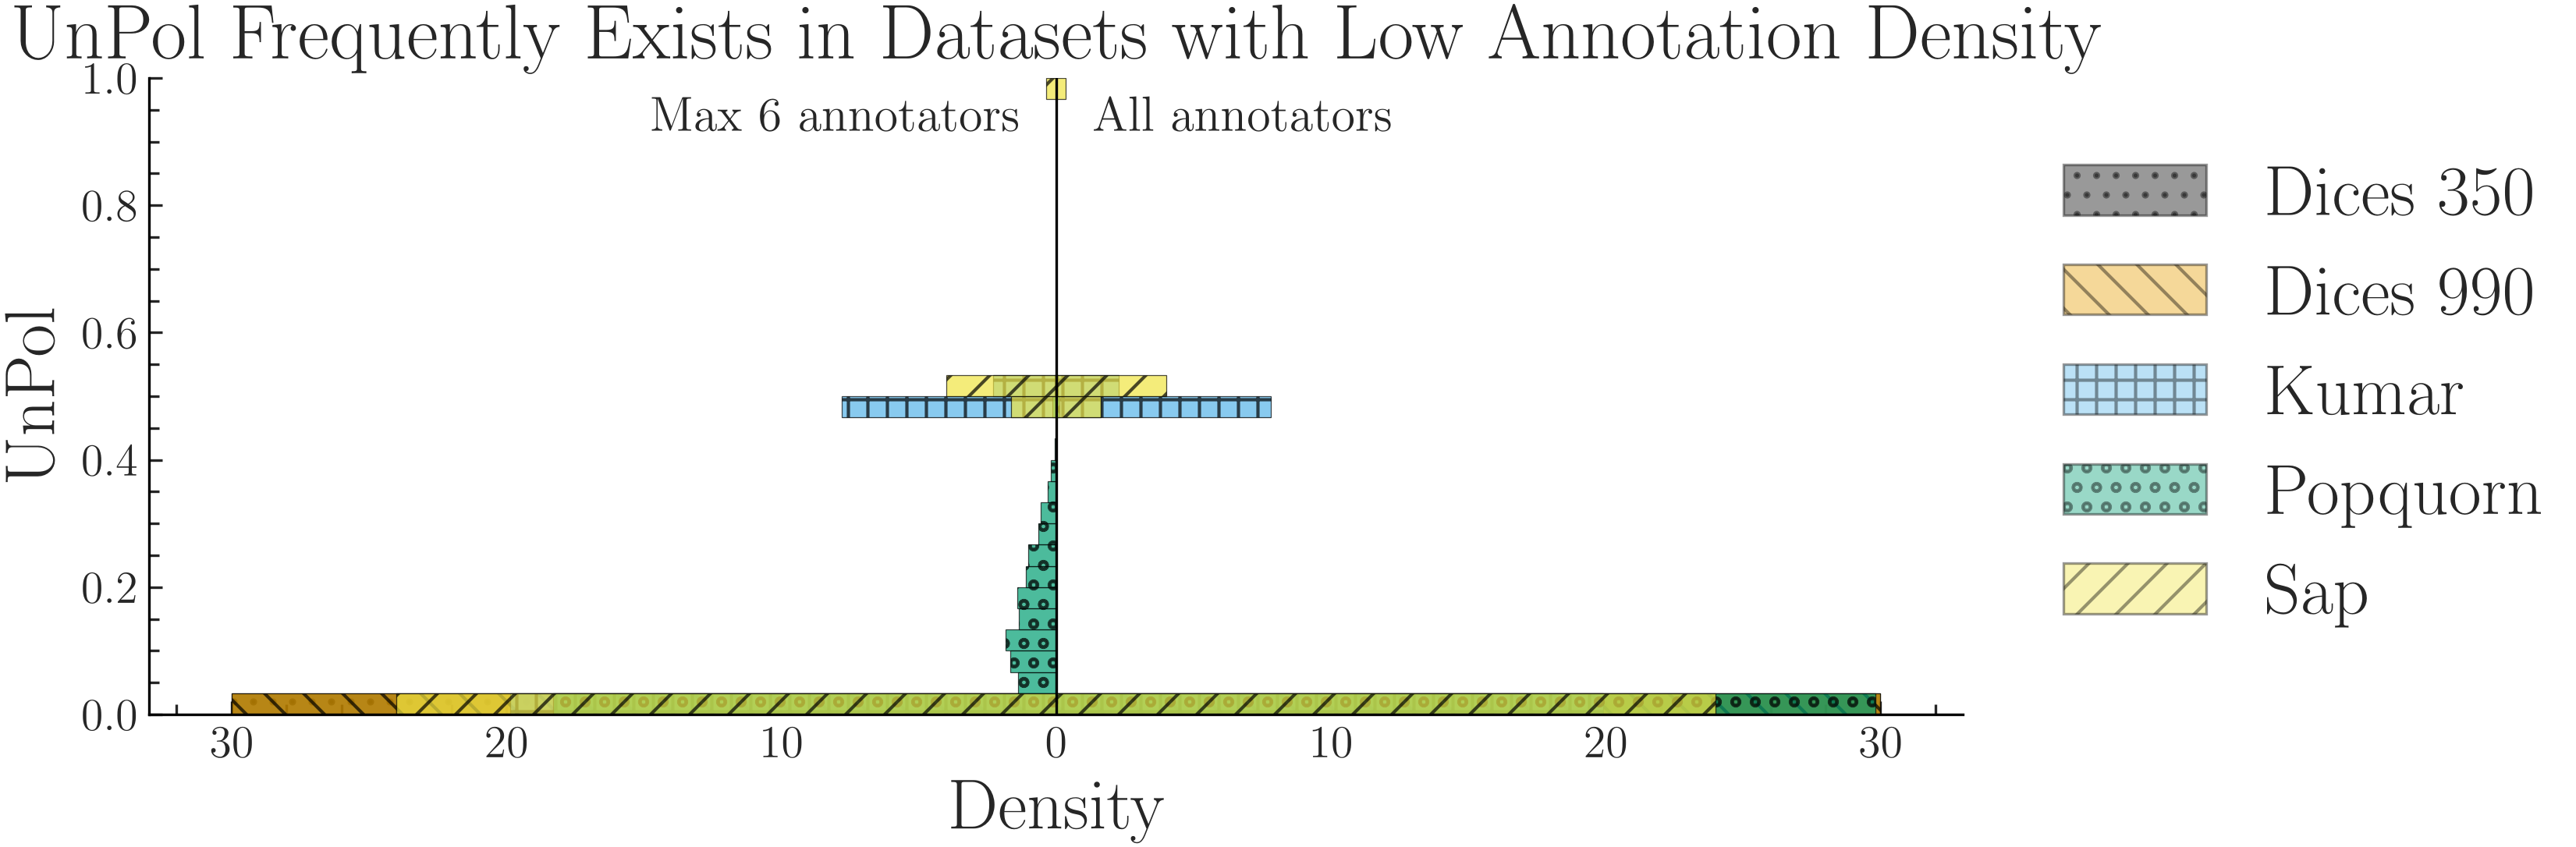
\includegraphics[width=\linewidth]{apriori.png}
	\caption{\ac{unpol} across our datasets (\S\ref{sec:datasets}). Contrary to assumptions made in prior work, \ac{unpol} is commonly non-zero and can even reach $\textit{nDFU} = 1$ in datasets with low annotator counts (see Table~\ref{tab:datasets}). The left side of the figure shows the same datasets, where annotations are subsampled 100 times down to six annotators and their \ac{unpol} is averaged.}
	\label{fig:inherent}
\end{figure}

\paragraph{Is All \ac{sysdis} Attributable to a \ac{sdd}?} In theory, we would expect all \ac{sysdis} to be attributable to some annotator \ac{sdd}, either one that is observed in our dataset, or latent (e.g., whether the annotators had lunch before their task). Some theoretical models such as \ac{au} make this assumption explicit, with \ac{au} attributing polarization to a \ac{sdd} only when all individual groups show completely unimodal annotation histograms. We posit that this is not the case when datasets are created using few annotators per item.

\paragraph{Definition} Formally, the \acf{unpol} for a single item $c$ is the minimum \ac{ndfu} exhibited by any arbitrary group (Eq.~\ref{eq:inherent}). When considered exhaustively, these theoretical, random splits produce both observed and latent groups. Since \ac{ndfu} operates only when a group has at least three annotators (Eq.~\ref{eq:ndfu}), this yields $\sum_{k=3}^{n} \binom{n}{k}$ possible groups, which is computationally intractable for large annotator counts. We can therefore use Monte Carlo sampling by drawing $k$ random partitions with random sizes (Eq.~\ref{eq:random}) which serves as an upper bound (as it considers a strict subset of Eq.~\ref{eq:inherent}).

\begin{multicols}{2}
	\noindent
	\begin{equation}
		\label{eq:inherent}
		\mathrm{Pol}_{inh}(c) = \min_{S \in G_c} \left\{ \mathrm{nDFU}(S) \right\}
	\end{equation}
	\begin{equation}
		\label{eq:random}
		\mathrm{Pol}_{inh}^{MC}(c) = \min_{j=1}^{k} \left\{ \mathrm{nDFU}(S_j) \right\}
	\end{equation}
\end{multicols}
\noindent where $G_c$ is the collection of all subsets $S$ of annotations for an item $c$ such that $\lvert S \rvert \ge 3$ and $S_j$ is a random sample drawn from $G_c$ for $j=1, \dots, k$.

\paragraph{Does It Exist?} We compute the \ac{unpol} for each item across the five datasets. For Sap and Kumar, we use the exhaustive formulation (Eq.~\ref{eq:inherent}), whereas for the two DICES datasets we rely on the Monte Carlo approximation with $k=1000$ (Eq.~\ref{eq:random}). Fig.~\ref{fig:inherent} shows that in all DICES items there exists at least one group that fully accounts for the observed \ac{ndfu} even when repeatedly subsampling down to six annotators.\footnote{$Pol_{inh}^{MC}(c)=0 \Rightarrow Pol_{inh}(c)=0$ due to Eq.~\ref{eq:random}, as is the case of increased $k$ in Eq.~\ref{eq:random}.}\footnote{See App.~\ref{app:ablation} for why this observation could be explained by DICES being structurally different.} Interestingly, this observation does not hold for the Kumar and Sap datasets, despite evaluating all possible annotator groups exhaustively. We also observe that \ac{unpol} typically exists on smaller annotation counts, as evidenced by POPQUORN in Fig~\ref{fig:inherent} and by LLM annotations only exhibiting \ac{unpol} when subsampling down to six annotators per item (App.~\ref{app:llms}; Fig.~\ref{fig:inherent-llms}). See App.~\ref{app:unpol}; Table~\ref{tab:inherent-examples} for examples of items with high \ac{unpol} and App.~\ref{app:llms}; Fig.~\ref{fig:inherent-llms} for \ac{unpol} exhibited by LLMs for each dataset and instruction prompt.

\begin{finding}
	\label{finding:inherent}
	Items may exhibit a degree of \ac{unpol} that cannot be attributed to any known or latent annotator grouping.
\end{finding}


\subsection{How Should We Design Subjective Datasets?}
Subjective datasets should be tailored to their specific use \citep{vidgen_2021_directions}, so using very large datasets for social science analysis may not be necessary \citep{rossi_2024}. While \ac{dc} may be convenient for training classifiers, relying on it without rigorous evaluation of \ac{sysdis} can lead to misconfigured or biased models \citep{sap-etal-2019-risk}, evaluation which is impossible without the necessary \ac{dc}). However, it comes at the expense of the other two (arguably more important) qualities. Generally, the \emph{easiest-to-use resources for training LLMs and classifiers may be the riskiest}, as meaningful, \ac{sysdis} cannot be reliably quantified (see the Kumar dataset in this study). We therefore recommend prioritizing dataset creation by first ensuring sufficient \ac{ad}, then achieving necessary \ac{gc} across underrepresented groups, and finally allowing budgetary constraints to determine \ac{dc}.

While this tension between the need for massive data volumes in AI training and the requirement of responsible social science to use deeply annotated, subjective datasets is unlikely to be resolved, a practical step is providing full annotation guidelines in both cases. If the annotation target and definitions are unknown, comparing results across different datasets becomes extremely difficult. As shown in \S\ref{sec:llms}, without clear guidelines, differences in polarization patterns remain obscured when analyzing data from multiple studies.


\section*{Conclusion}
In this study, we showed that current disagreement attribution measures tend to underperform in realistic annotation settings through a large scale empirical study. We designed a new measure which quantifies attribution of \acf{sysdis} to annotator \acp{sdd}, taking into account the limitations of real-life annotation datasets. Using this measure, we identified shared polarization patterns among gender and ethnicity groups across five subjective \ac{nlp} datasets. Additionally, we found that LLM annotators can create polarized annotations, but do not reproduce human polarization patterns, even when using prompt engineering. Our research is limited due to the information present in the datasets; namely, we discovered that due to low annotation counts per item, some polarization cannot be attributed to any combination of theoretical dimensions (``\acf{unpol}''). Overall, our work warns against using LLM persona prompting without rigorous, task-specific evaluation, and motivates the development of ``wider'' datasets with fewer but better annotated items.


\section*{AI Use Statement}
In this work we used proprietary models such as Anthropic's Claude Sonnet 5 and OpenAI's GPT-5 for partially implementing the synthetic experiments in \S\ref{sec:methods} and generating parts of the library, experiment and graph-creation code. The unit-tests used in our library were similarly generated by these models, although new tests were added as edge-cases and bugs were discovered. All such tasks were executed with direct author supervision, and all relevant code files (library, experiments, graphs) have been edited manually at multiple points by the authors to ensure reproducibility, accuracy and software quality. We also used Scholar Labs to find citations for targeted claims (e.g., for known issues with persona prompting), although all such citations were manually filtered by us. Finally, we used a locally hosted Gemma-4 model (specifically the \texttt{gemma-4-E4B-it-Q4\_K\_M.gguf} variant) for rephrasing this manuscript in order to improve readability. We take responsibility for the final content of this work, including text, claims or artifacts produced with the aid of generative AI.


\section*{Ethics Statement}

\paragraph{Dual Use Concerns} The primary objective of this study is to identify systemic sources of \ac{sysdis} in subjective \ac{nlp} datasets to facilitate the construction of more fair and reliable AI systems. However, given that our methodology allows for the quantitative attribution of specific annotation patterns to \acp{sdd}, we acknowledge three primary risks inherent in this research.
\begin{enumerate*}
	\item \emph{Discriminatory Profiling}: If the measure is applied outside of a dataset quality analysis, its ability to correlate specific opinion patterns with annotator groups could be misused for surveillance or unjust profiling.
	\item \emph{Automated Bias Amplification}: The diagnostic patterns of disagreement we detect are reflections of human systemic biases. Without human oversight, training subsequent models on these patterns risks automating and entrenching existing societal prejudices.
	\item The knowledge provided by \emph{apunim} could be \emph{weaponized}, allowing malicious actors to strategically target weak points in moderation systems or intentionally maximize societal conflict.
\end{enumerate*}
We stress that our measure functions strictly as a diagnostic warning signal. Any deployment in a real-world system must mandate a human-in-the-loop review, ensuring that identified patterns lead to systemic improvements (e.g., policy reform, demographic diversity initiatives) rather than merely justifying an automated system. In any case, despite the risks, we believe that the benefits of this research outweigh the risks outlined above.

\paragraph{Data Sourcing and Privacy} All datasets employed in this study were either publicly accessible or provided to us by the original authors with full disclosure regarding the purpose of our research. No identifiable, personal information was included in our pipeline. We do not release proprietary data provided by the authors, nor have we provided any to proprietary LLMs. Finally, we note that our data is limited to English posts from a U.S. cultural context and our results may not be representative for other cultures.

\paragraph{Examples Used} Our study utilizes examples of comments that may be considered divisive across certain demographics. These examples were generated by our team solely for demonstration purposes. We explicitly state that the contents of these examples and the groups studied do not necessarily reflect the views or behaviors of the groups they represent, nor do they reflect the opinions of the authors. We have partially censored explicit slurs in Table~\ref{tab:inherent-examples} in order to both mitigate uncomfortable or triggering content, while also showing enough content for the examples to be effective.

\paragraph{Prompts Used} This study uses adversarial prompts which explicitly instruct the model to change its outputs according to their persona prompts. The purpose of these prompts is to test the LLMs under an extreme case of prompt engineering and are not to be used for generalized usage. The use of these prompts may degrade model performance, increase the risk of stereotyping and produce misleading results.


\appendix

\section {Acronyms}

\begin{acronym}[WWW]
	\acro{iaa}[IAA]{Inter-Annotator Agreement}
	\acro{sdd}[SDD]{SocioDemographic Dimension}
	\acro{au}[AU]{A Posteriori Unimodality}
	\acro{sysdis}[SysDis]{Systematic Disagrement}
	\acro{unpol}[UnPol]{Unnatributtable Polarization}
	\acro{ndfu}[nDFU]{normalized Distance From Unimodality}
	\acro{nlp}[NLP]{Natural Language Processing}
	\acro{gpl}[GPLv3]{GNU General Public Licence v3}
	\acro{aa}[AA]{African American}
	\acro{hs}[HS]{Hate Speech}
	\acro{sd}[SD]{Standard Deviation}
	\acro{dc}[DC]{Data Coverage}
	\acro{gc}[GC]{Group Coverage}
	\acro{ad}[AD]{Annotation Density}
\end{acronym}


\section{Exploratory Analysis}
\label{app:ann_details}

The number of annotators per item for all datasets presented in \S\ref{sec:datasets} can be found in Fig.~\ref{fig:ann_counts}, and descriptive statistics can be found in Table~\ref{tab:num-annot}. The DICES-990 dataset has exactly 123 annotations per item, while the other datasets exhibit a few variations around the central mean reported in Table~\ref{tab:datasets}. Interestingly, the sample used from the Kumar dataset exhibits a few items that vastly exceed the promised $5$ number of annotators. We do not include these items, since they are very likely a data error. Tables~\ref{tab:dices-stats},\ref{tab:sap-stats},\ref{tab:kumar-stats} show the annotation counts for each \ac{sdd} group in each dataset.


\begin{figure}[t]
	\centering
	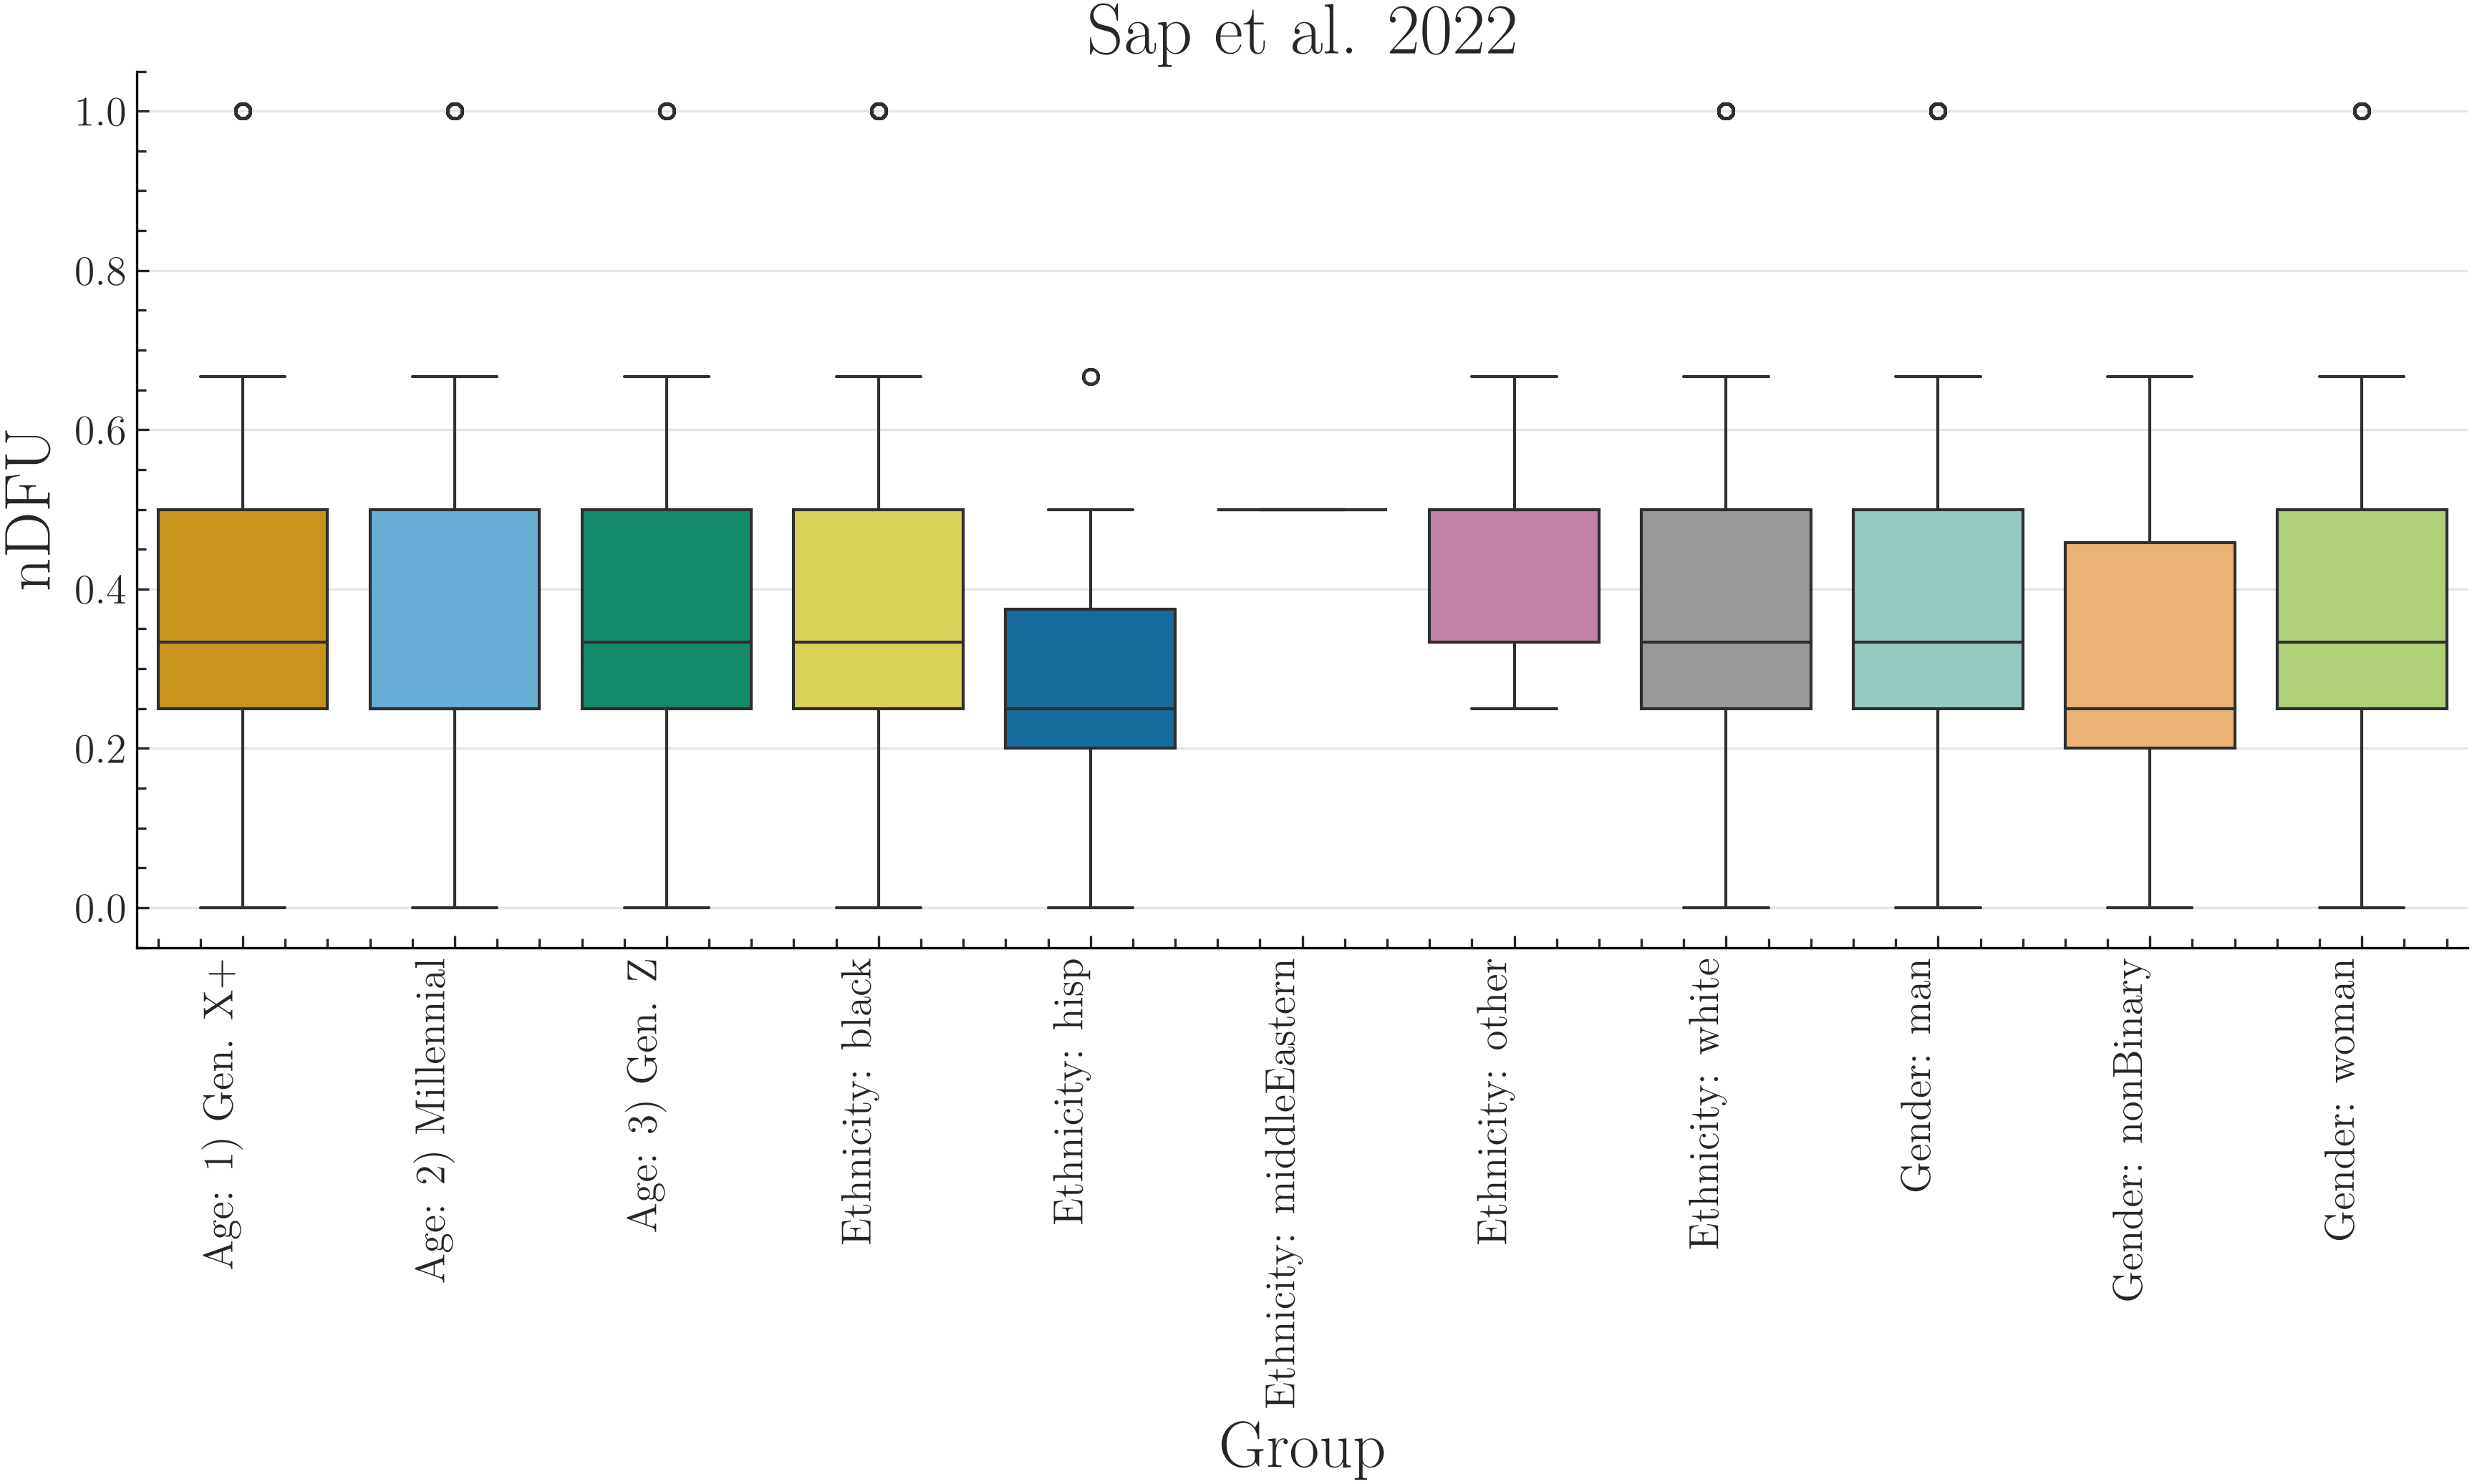
\includegraphics[width=0.48\linewidth]{sap.png}
	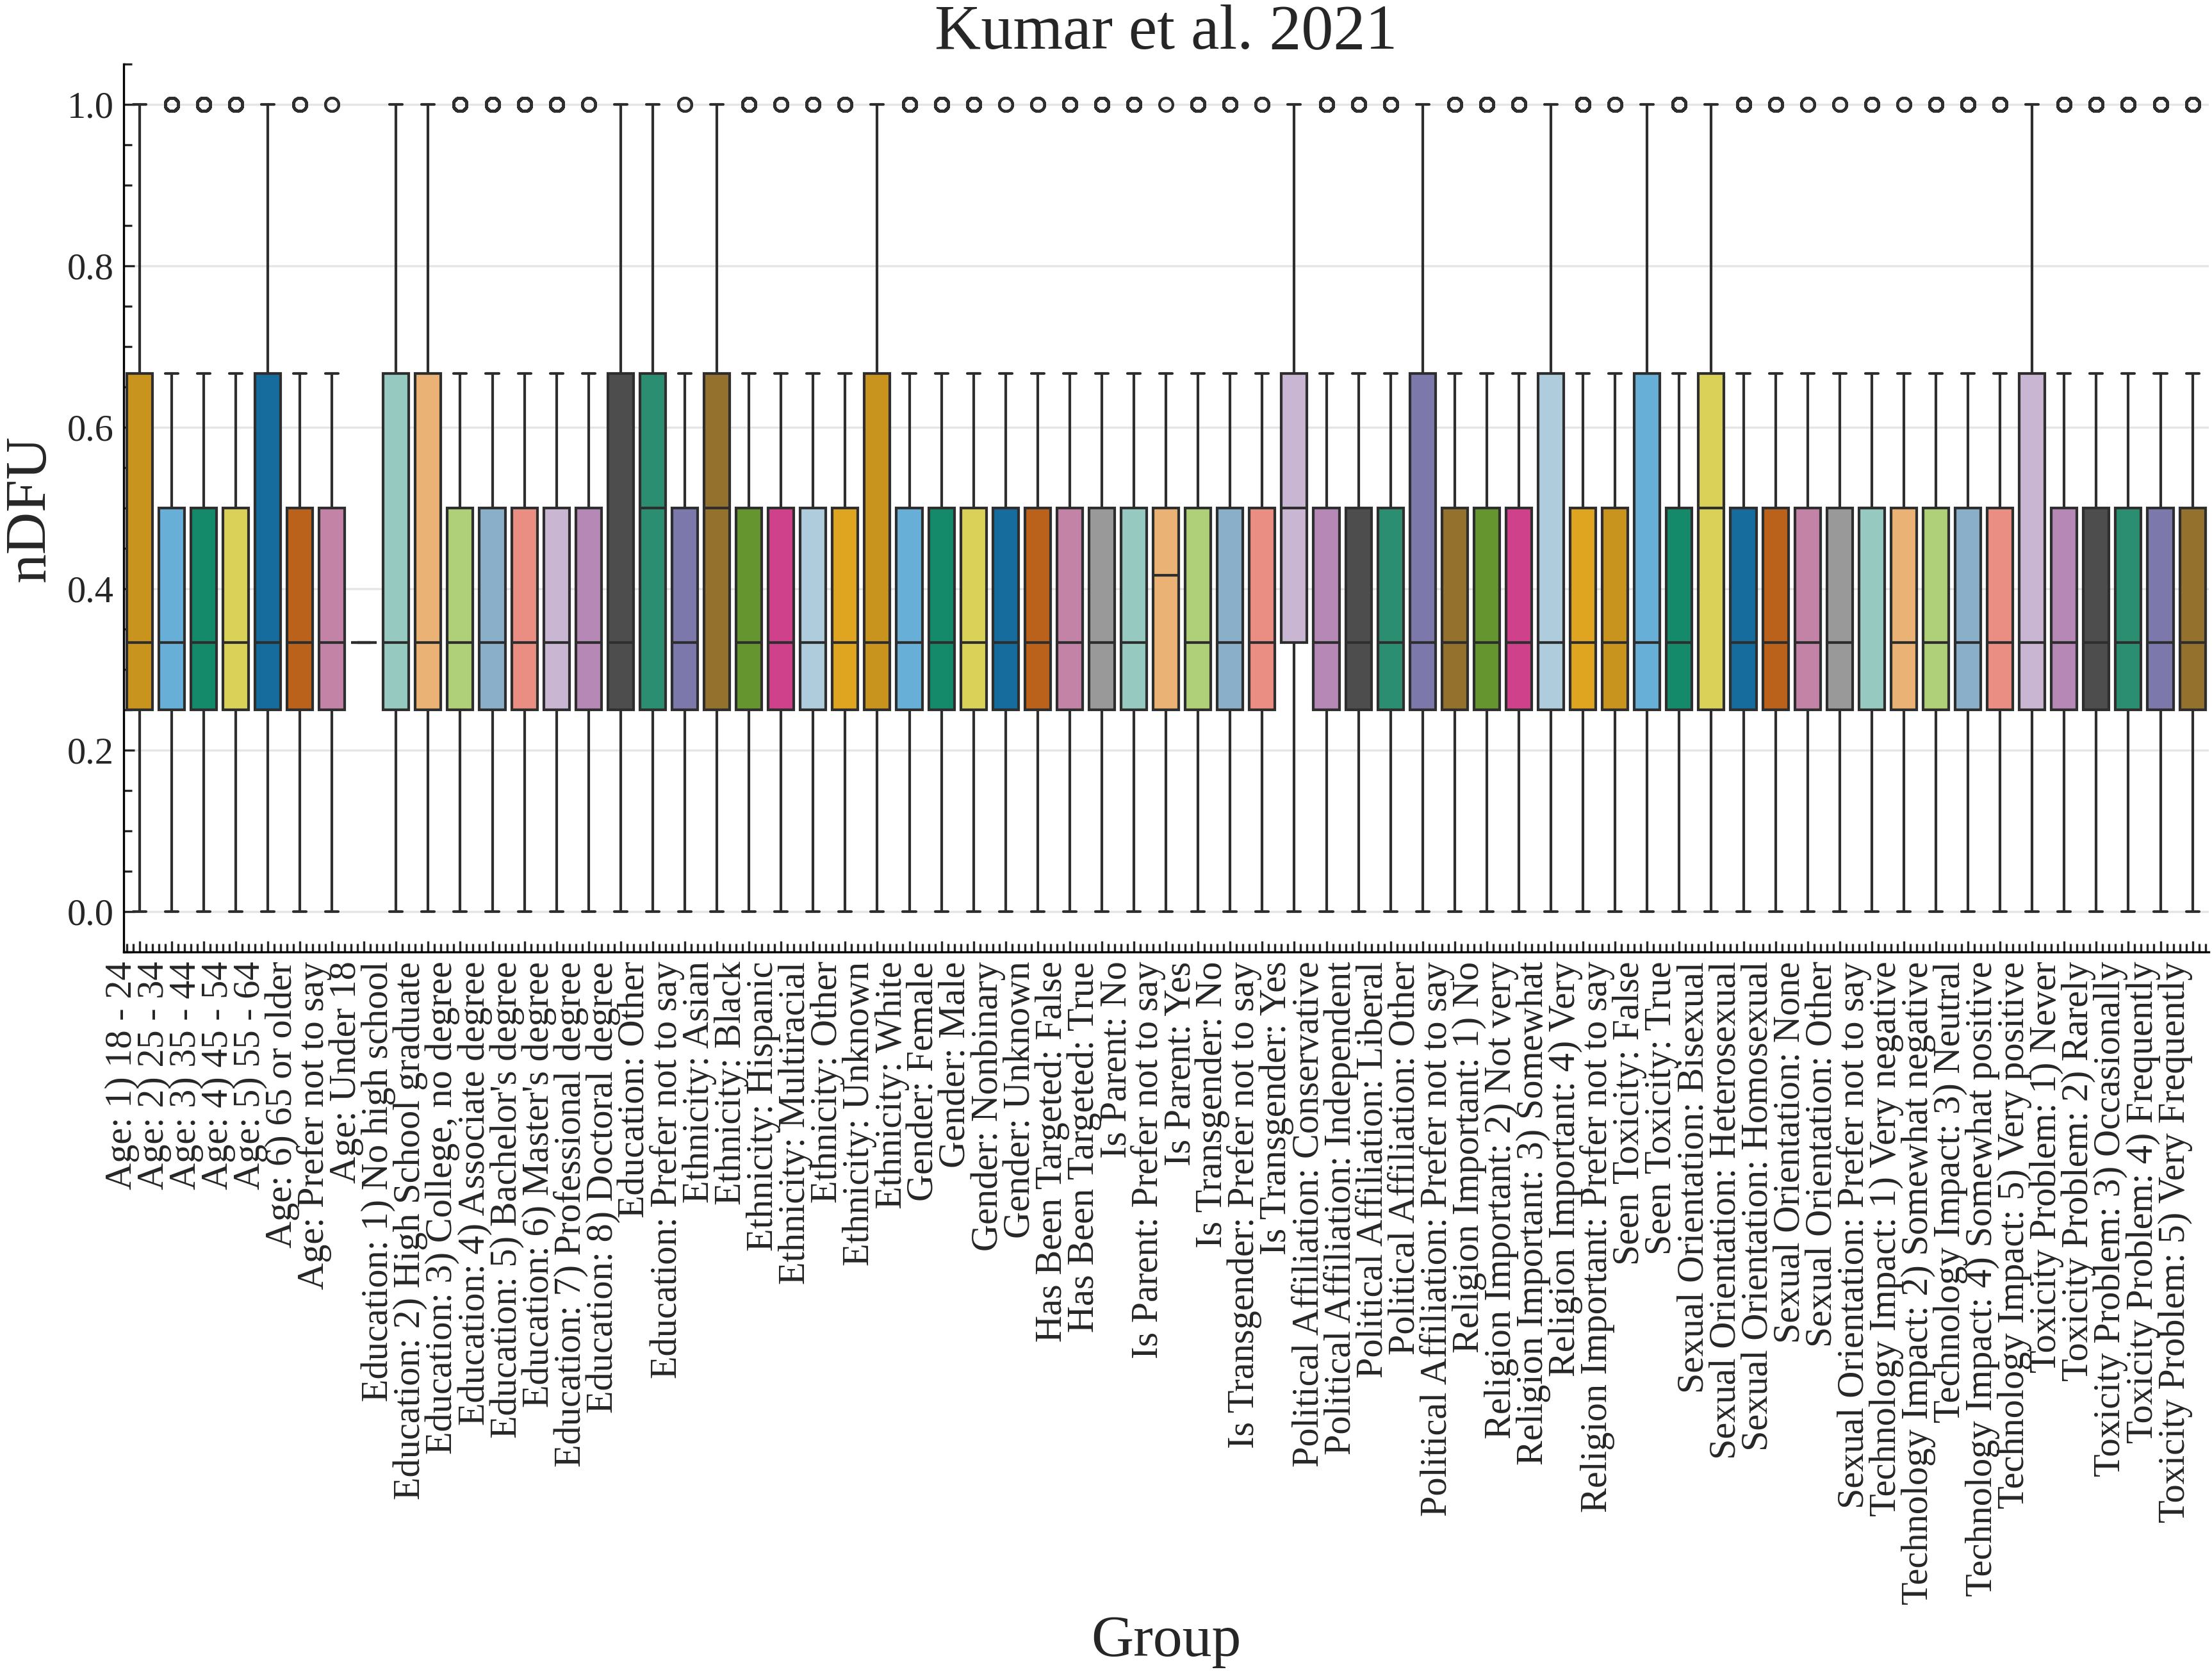
\includegraphics[width=0.48\linewidth]{kumar_sample.png}
	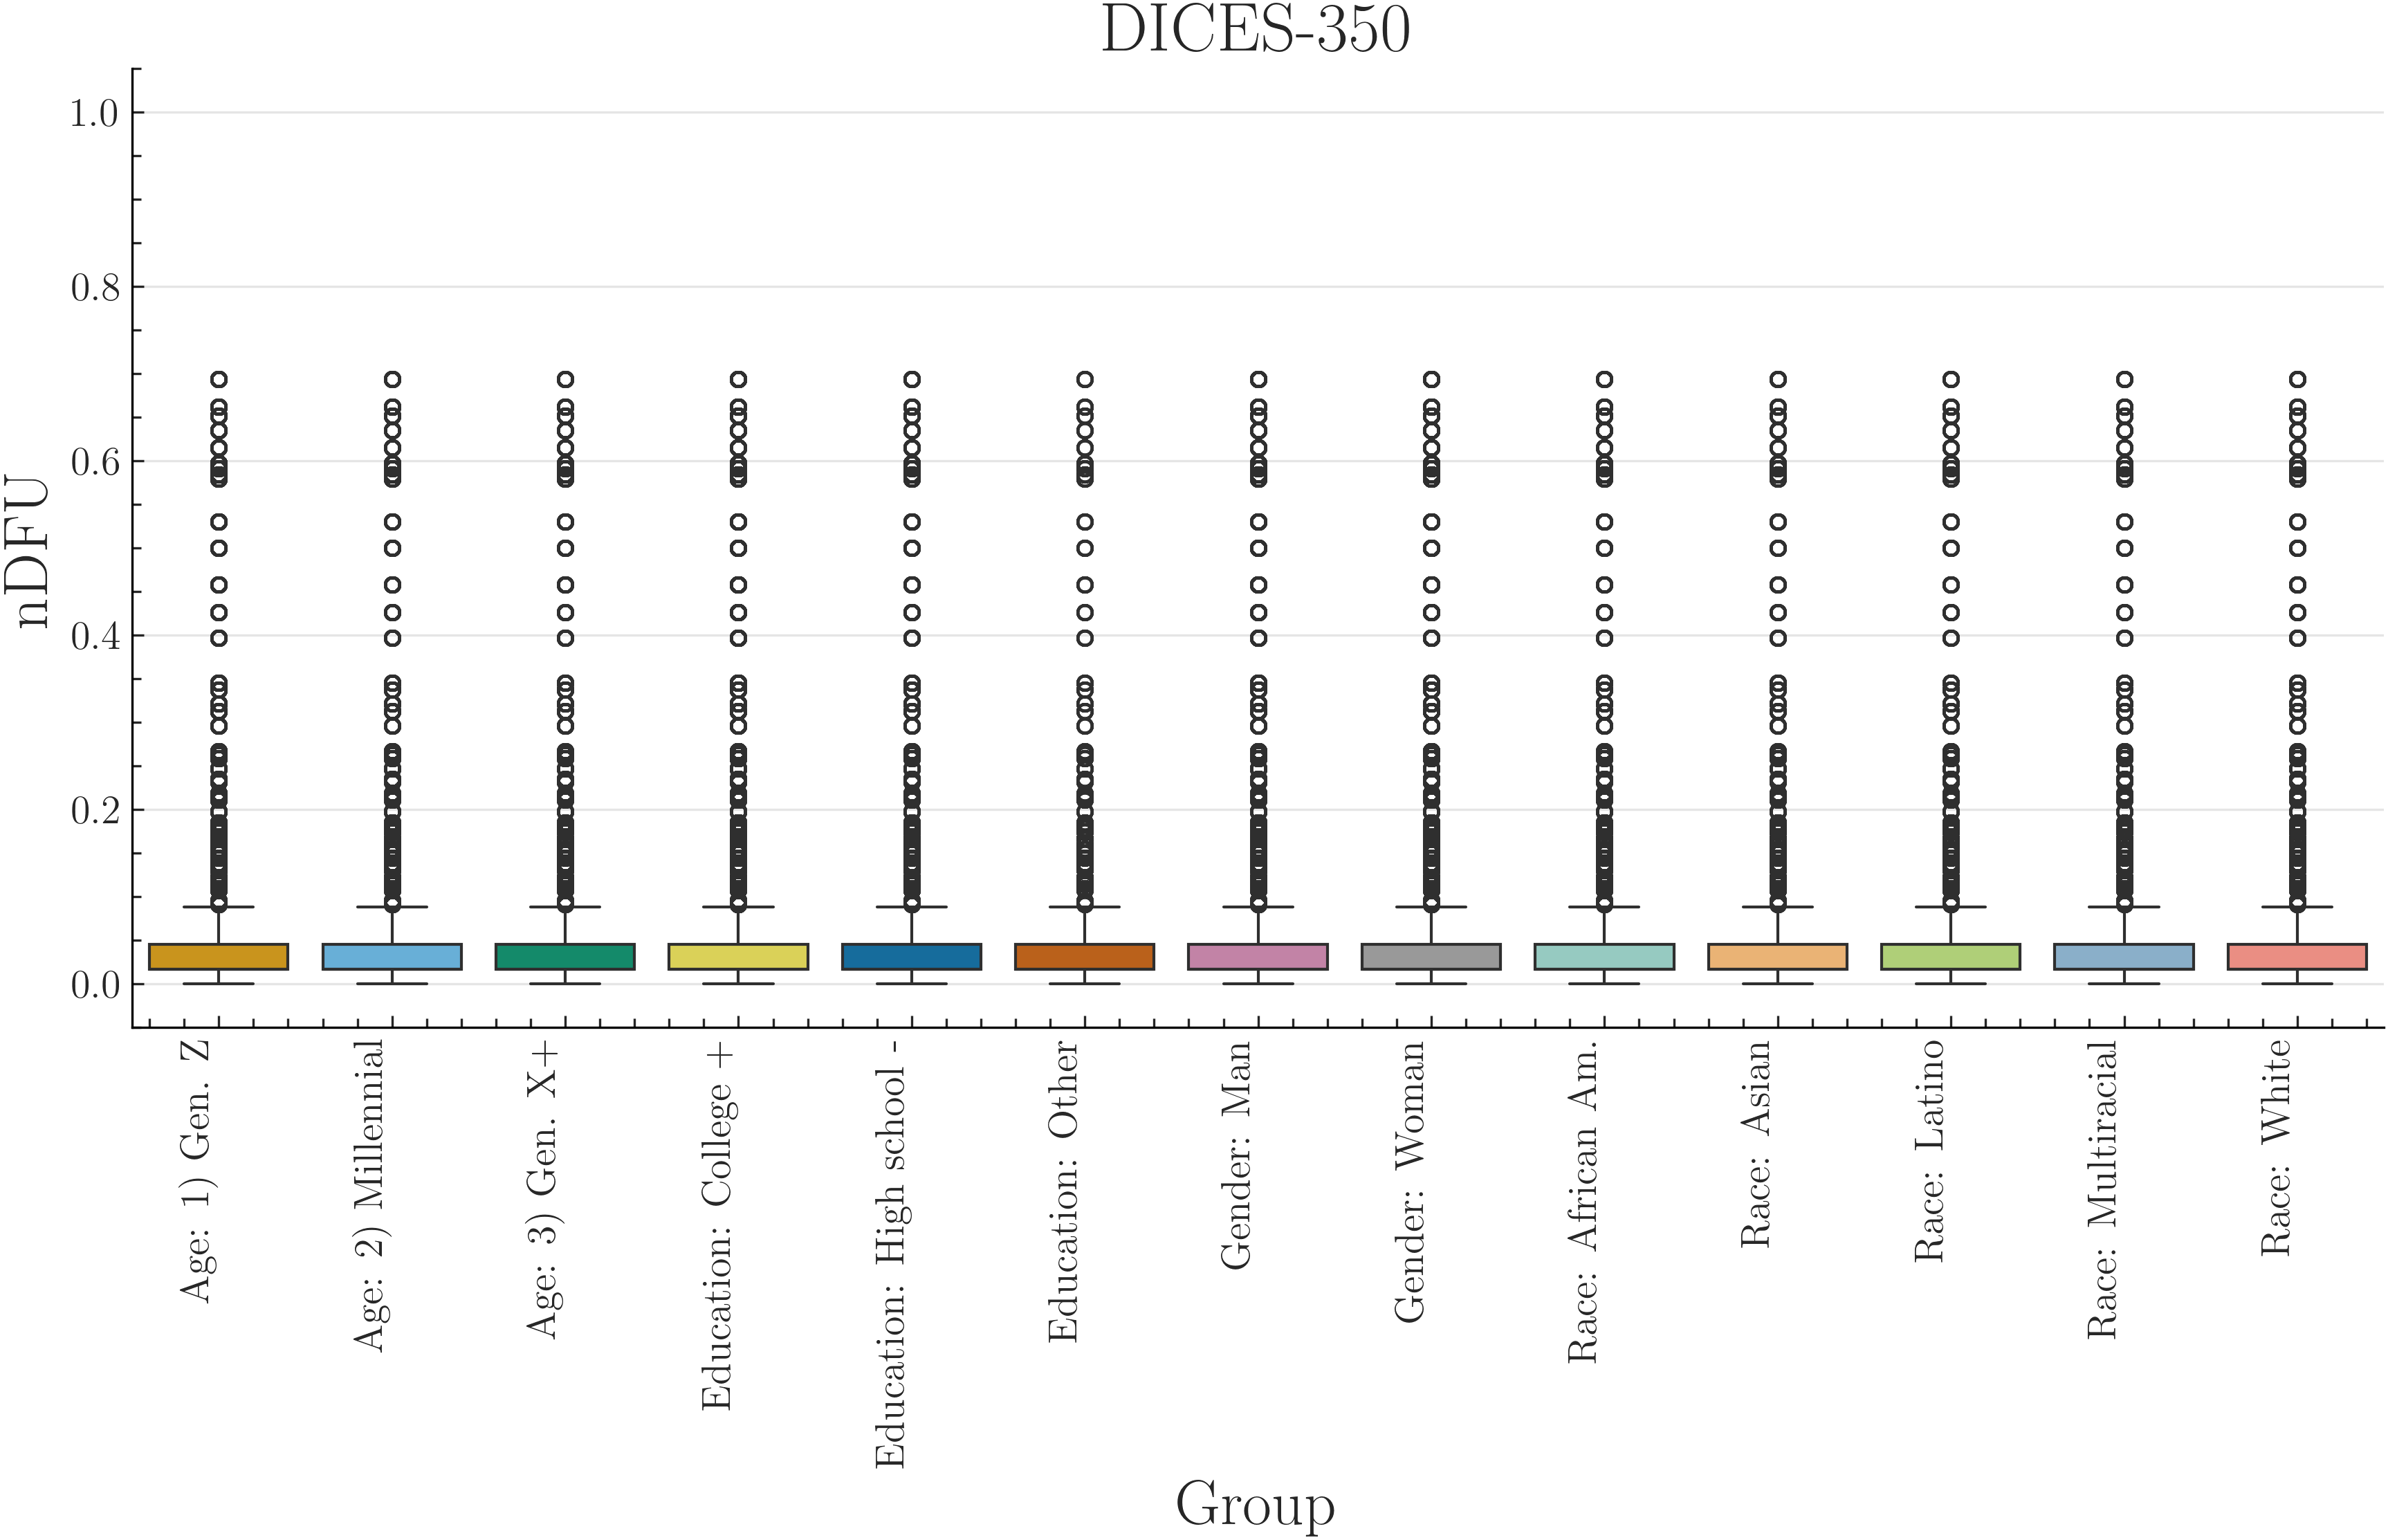
\includegraphics[width=0.48\linewidth]{dices-350.png}
	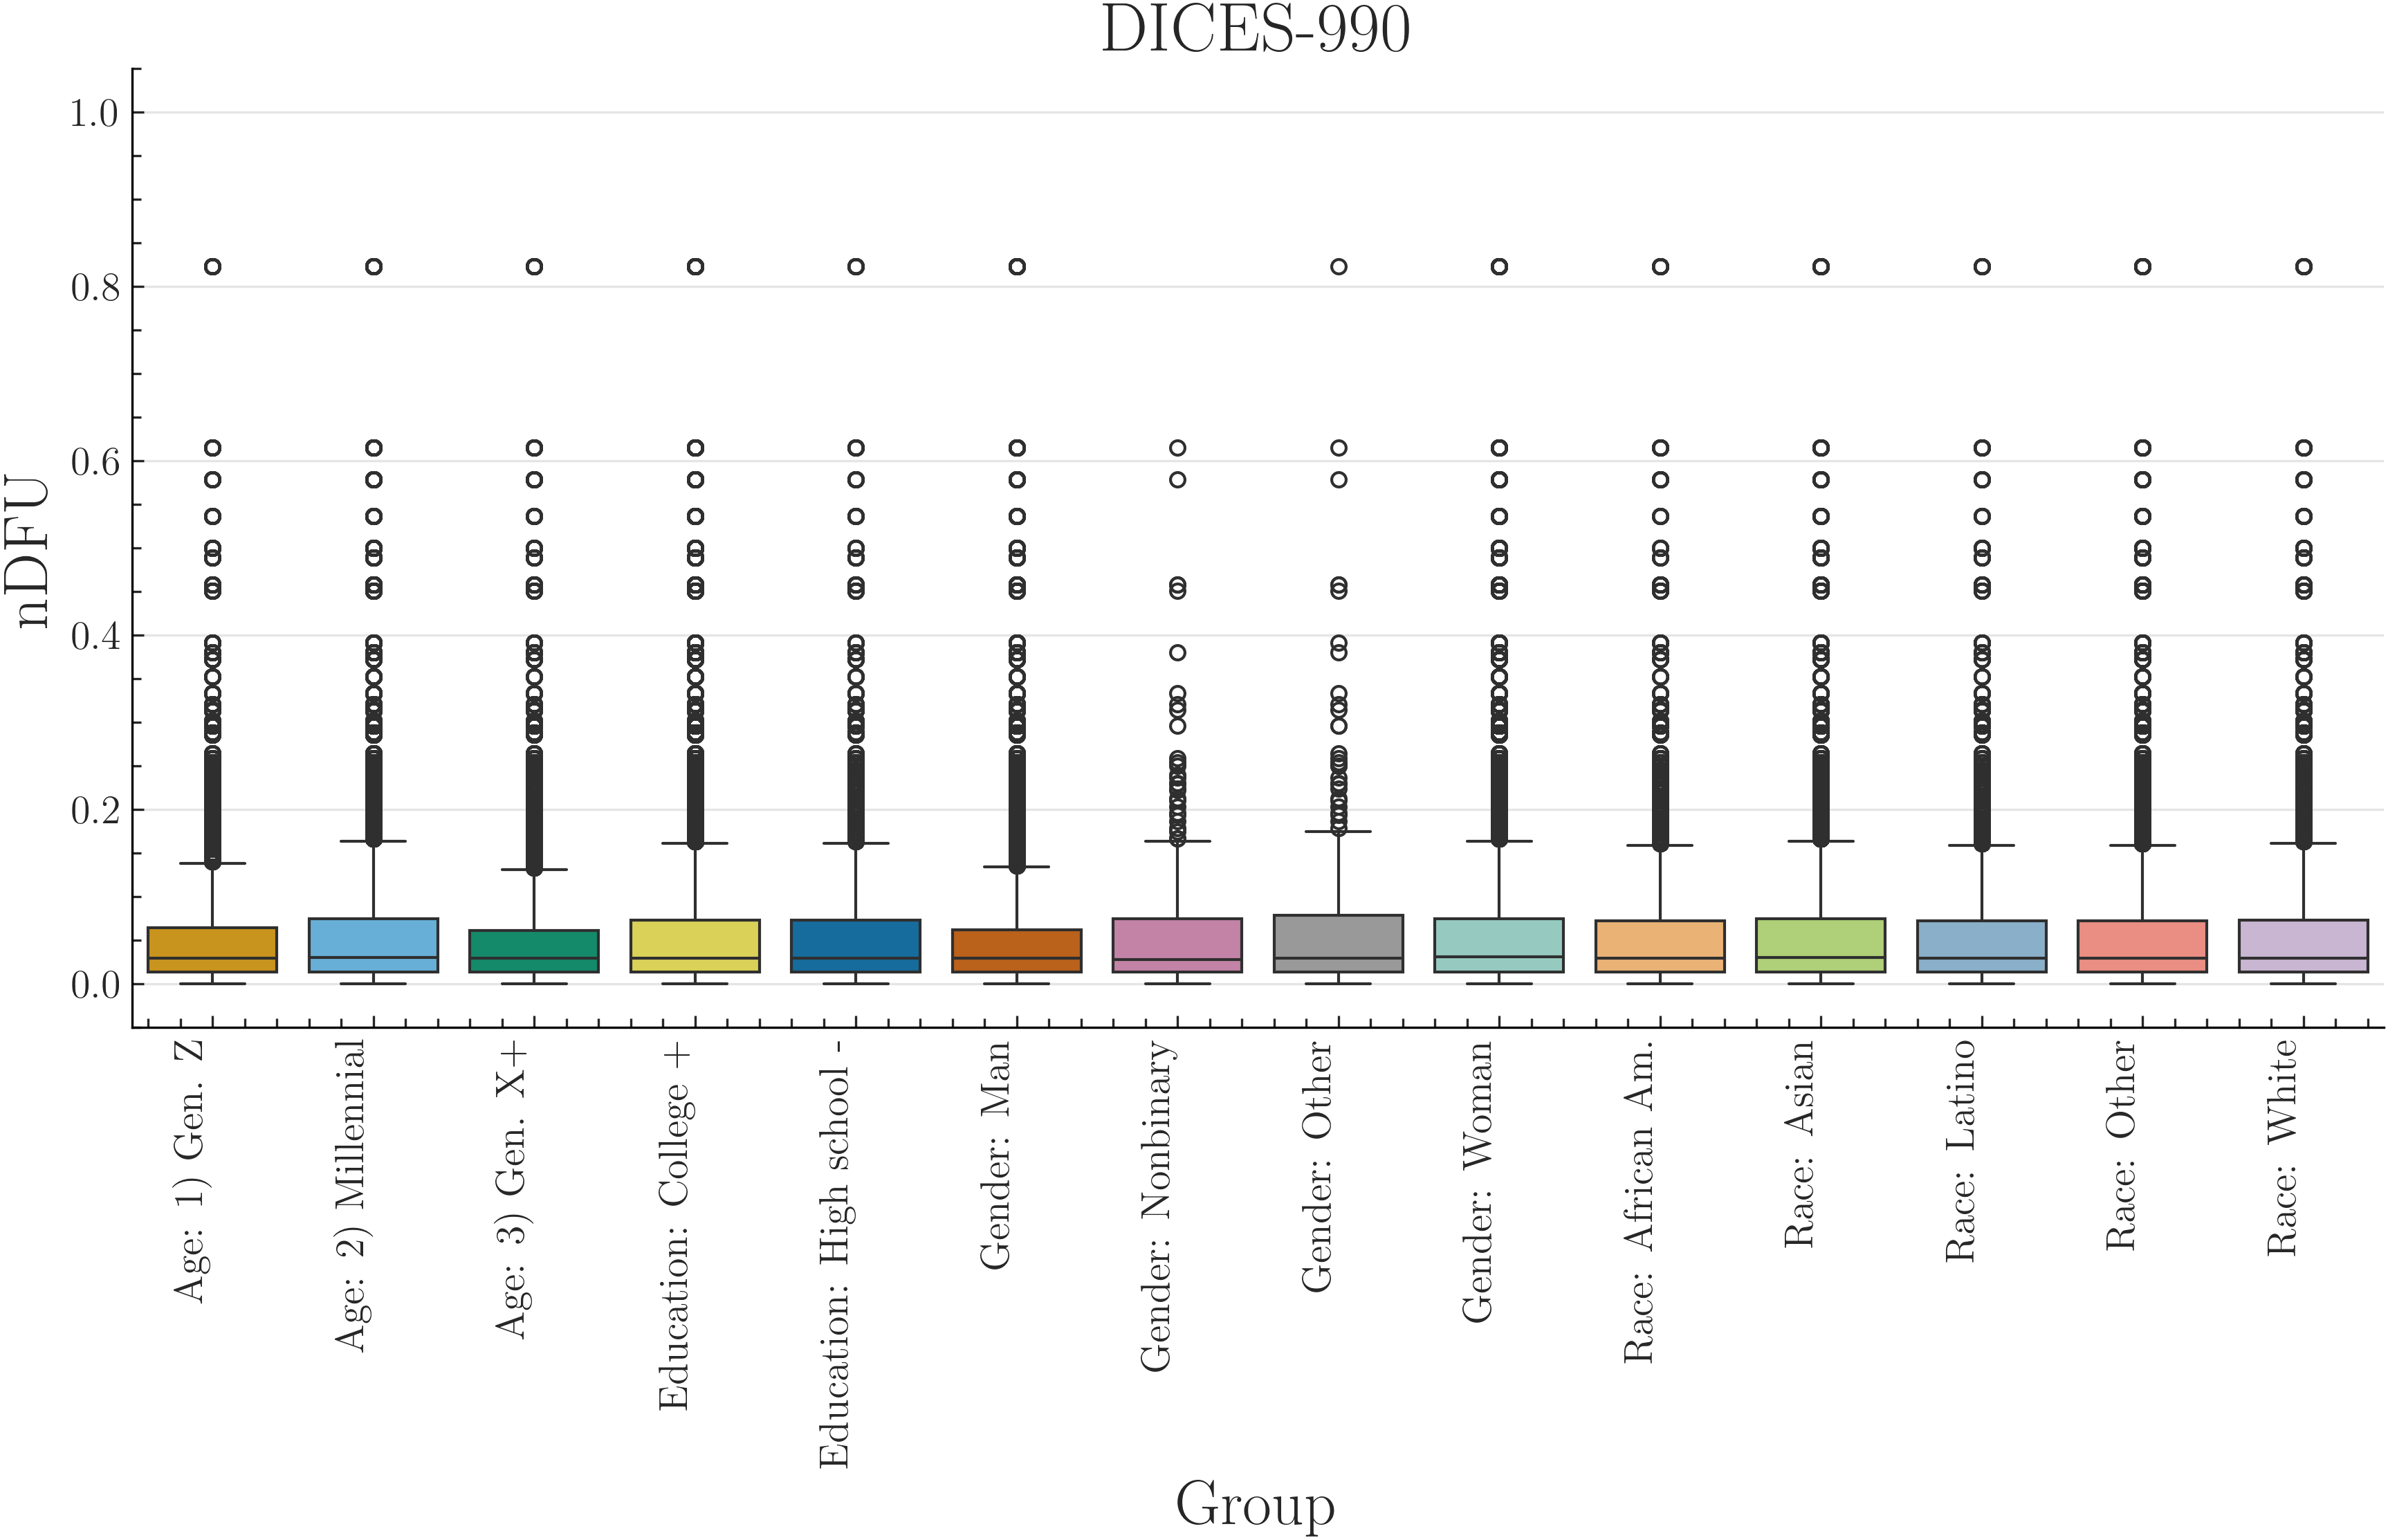
\includegraphics[width=0.48\linewidth]{dices-990.png}
	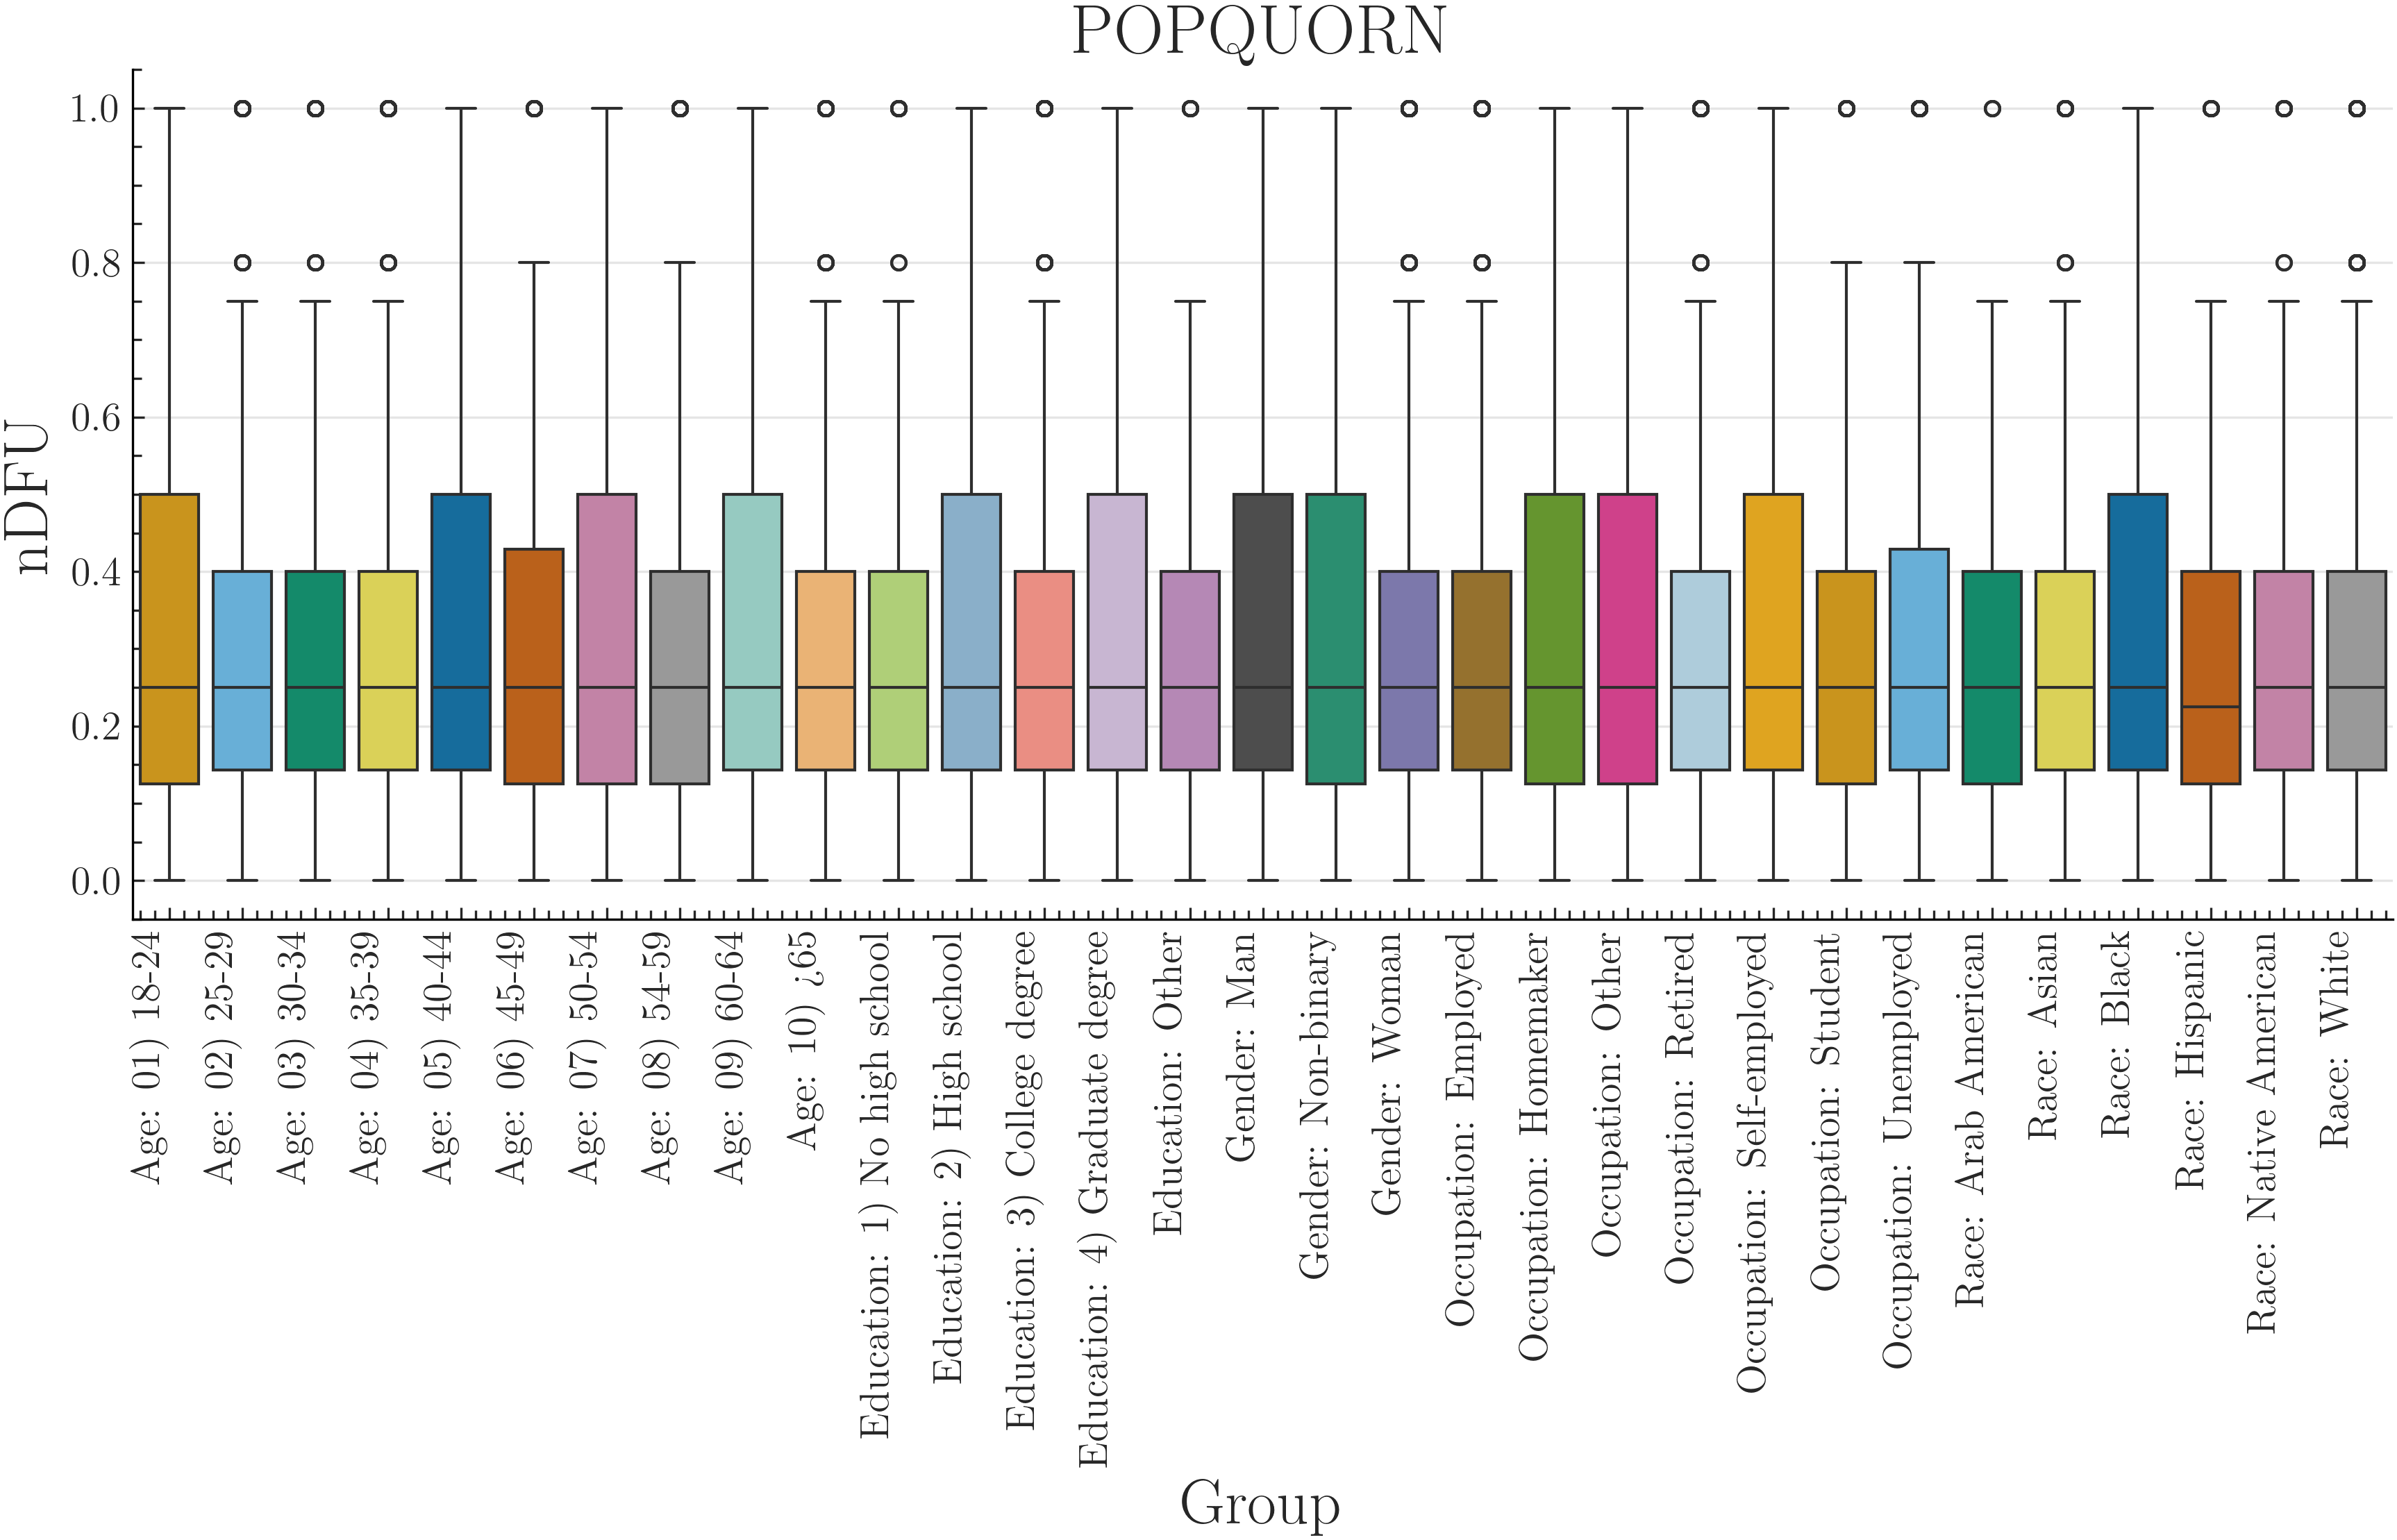
\includegraphics[width=0.48\linewidth]{popquorn.png}
	\caption{Boxplots of dataset polarization for the human datasets considered in this paper for all groups in each examined \ac{sdd}.}
	\label{fig:dataset-polarization}
\end{figure}


\begin{figure}[t]
	\centering
	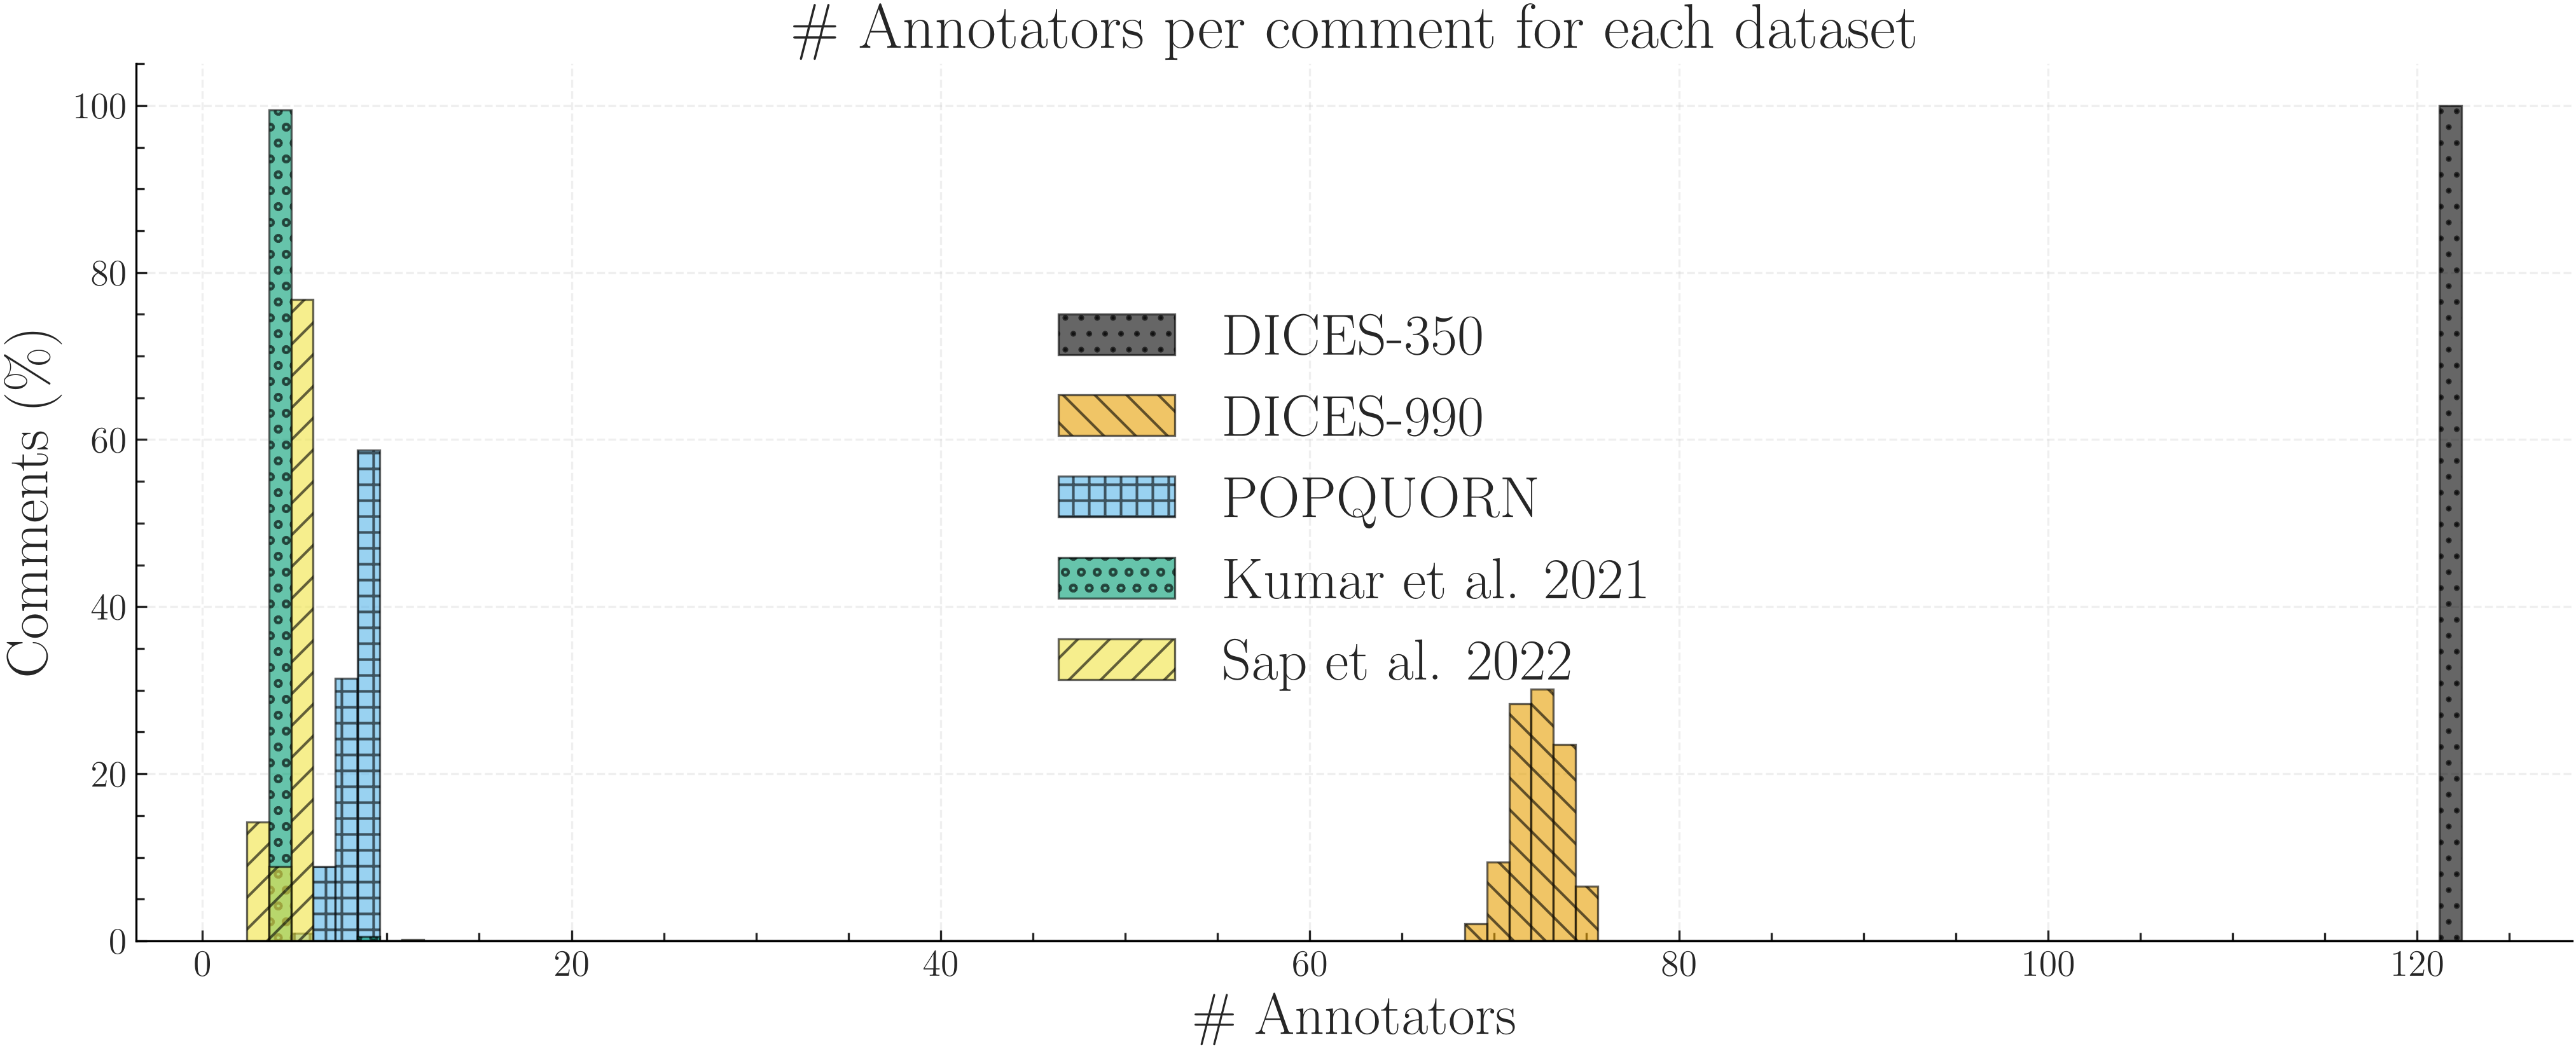
\includegraphics[width=0.8\linewidth]{annotator_count_histogram.png}
	\caption{We calculate the ratio of items for each dataset (y-axis) that had $x$ number of annotators (x-axis). We truncate the x-axis to 130 annotators, disregarding very few items in the Kumar dataset exceeding this threshold (see Table~\ref{tab:num-annot}), which is likely caused by a data error.}
	\label{fig:ann_counts}
\end{figure}


\begin{table*}[t]
	\centering
	\caption{Descriptive statistics for the number of annotations per comment, grouped by dataset.}
	\label{tab:num-annot}
	\begin{tabular}{lrrrrrrrr}
		\toprule
		& count & mean & std & min & 25\% & 50\% & 75\% & max \\
		\midrule
		DICES-350 & 350 & 123 & 0 & 123 & 123 & 123 & 123 & 123 \\
		DICES-990 & 990 & 72.8313 & 1.1652 & 69 & 72 & 73 & 74 & 76 \\
		POPQUORN & 1500 & 8.6573 & 0.9087 & 5 & 8 & 9 & 9 & 10 \\
		Kumar & 105910 & 5.0261 & 0.3604 & 5 & 5 & 5 & 5 & 10 \\
		Sap & 585 & 5.6359 & 0.7713 & 3 & 6 & 6 & 6 & 12 \\
		\bottomrule
	\end{tabular}
\end{table*}


\begin{table}[t]
	\caption{Subgroup Counts for DICES-990 (left) and DICES-350 (right). ``Support'' refers to annotation count.}
	\label{tab:dices-stats}
	\small
	\centering
	\begin{minipage}[t]{0.485\linewidth}
			\begin{tabular}{llc}
				\toprule
				\textbf{Category} & \textbf{Subgroup} & \textbf{Support} \\
				\midrule
				Gender & Woman & 36050 \\
				& Man & 35392 \\
				& Nonbinary & 331 \\
				& Other & 330 \\
				\midrule
				Race & Other & 26394 \\
				& Asian & 19885 \\
				& White & 12322 \\
				& Latino & 7170 \\
				& African Am. & 6332 \\
				\midrule
				Age & Gen. Z & 14899 \\
				& Millennial & 41542 \\
				& Gen. X+ & 15662 \\
				\midrule
				Education & College + & 64054 \\
				& High school - & 8049 \\
				\bottomrule
			\end{tabular}
	\end{minipage}
	\begin{minipage}[t]{0.45\linewidth}
			\begin{tabular}{llc}
				\toprule
				\textbf{Category} & \textbf{Subgroup}  & \textbf{Support}\\
				\midrule
				Gender & Woman & 21700 \\
				& Man & 21350 \\
				\midrule
				Race & White & 10500 \\
				& African Am. & 10150 \\
				& Asian & 9100 \\
				& Latino & 7700 \\
				& Multiracial & 5600 \\
				\midrule
				Age & 1) Gen. Z & 19600 \\
				& 2) Millennial & 12600 \\
				& 3) Gen. X+ & 10850 \\
				\midrule
				Education & College + & 26250 \\
				& High school - & 14350 \\
				& Other & 2450 \\
				\bottomrule
			\end{tabular}
	\end{minipage}
\end{table}

\begin{table}[t]
	\caption{Subgroup Counts for the Sap (left) and POPQUORN (right) datasets. ``Support'' refers to annotation count.}
	\label{tab:sap-stats}
	\centering
	\begin{minipage}[t]{0.45\linewidth}
		\begin{tabular}{llc}
			\toprule
			\textbf{Category} & \textbf{Subgroup} & \textbf{Support}\\
			\midrule
			Age& Gen. Z & 252 \\
			& Millennial & 2259 \\
			& Gen. X+ & 786 \\
			\midrule
			Race & White & 2168 \\
			& Black & 1091 \\
			& Hisp & 32 \\
			& Other & 5 \\
			& MiddleEastern & 1 \\
			\midrule
			Gender & man & 1859 \\
			& woman & 1412 \\
			& nonBinary & 26 \\
			\bottomrule
		\end{tabular}
	\end{minipage}
	\begin{minipage}[t]{0.485\linewidth}
		\begin{tabular}{llc}
			\toprule
			\textbf{Category} & \textbf{Subgroup} & \textbf{Count}\\
			\midrule
			Gender & Woman & 6470 \\
			& Man & 6166 \\
			& Non-binary & 350 \\
			\midrule
			Race & White & 9754 \\
			& Black & 1685 \\
			& Asian & 949 \\
			& Native American & 299 \\
			& Hispanic & 250 \\
			& Arab American & 49 \\
			\midrule
			Age & 18-24 & 1545 \\
			& 25-29 & 1236 \\
			& 30-34 & 1494 \\
			& 35-39 & 1547 \\
			& 40-44 & 1142 \\
			& 45-49 & 1091 \\
			& 50-54 & 947 \\
			& 54-59 & 1793 \\
			& 60-64 & 747 \\
			& >65 & 1444 \\
			\midrule
			Education & No high school & 237 \\
			& High school & 3934 \\
			& College degree & 6036 \\
			& Graduate degree & 2481 \\
			& Other & 298 \\
			\midrule
			Occupation & Student & 995 \\
			& Homemaker & 594 \\
			& Retired & 1446 \\
			& Employed & 6325 \\
			& Self-employed & 1692 \\
			& Unemployed & 1684 \\
			& Other & 250 \\
			\bottomrule
		\end{tabular}
	\end{minipage}
\end{table}

\begin{table}[t]
	\caption{Subgroup Counts for the Kumar dataset. ``Support'' refers to annotation count.}
	\label{tab:kumar-stats}
	\small
	\centering
	\begin{minipage}[t]{0.45\linewidth}

		\begin{tabular}{llc}
			\toprule
			\textbf{Category} & \textbf{Subgroup} & \textbf{Support}\\
			\midrule
			\multirow{4}{*}{Gender} & Female & 8011 \\
			& Male & 6832 \\
			& Unknown & 124 \\
			& Nonbinary & 93 \\
			\midrule
			\multirow{7}{*}{Ethnicity} & White & 10699 \\
			& Black & 1940 \\
			& Asian & 862 \\
			& Multiracial & 664 \\
			& Hispanic & 418 \\
			& Other & 247 \\
			& Unknown & 230 \\
			\midrule
			\multirow{9}{*}{Age} & Under 18 & 3 \\
			& 18 - 24 & 1711 \\
			& 25 - 34 & 5969 \\
			& 35 - 44 & 3785 \\
			& 45 - 54 & 1977 \\
			& 55 - 64 & 1101 \\
			& 65 or older & 471 \\
			& N/A & 43 \\
			\midrule
			\multirow{10}{*}{Education} & No high school & 71 \\
			& High School & 1353 \\
			& College & 3090 \\
			& Associate's & 1676 \\
			& Bachelor's & 6071 \\
			& Master's & 2261 \\
			& Professional & 236 \\
			& Doctoral & 198 \\
			& N/A & 71 \\
			& Other & 32 \\
			\midrule
			\multirow{5}{*}{Sexual Orient.} & Heterosexual & 12391 \\
			& Bisexual & 1665 \\
			& Homosexual & 515 \\
			& N/A & 302 \\
			& Other & 131 \\
			\bottomrule
		\end{tabular}
	\end{minipage}
	\begin{minipage}[t]{0.485\linewidth}
		\begin{tabular}{llc}
			\toprule
			\textbf{Category} & \textbf{Subgroup} & \textbf{Support}\\
			\midrule
			\multirow{3}{*}{Is Trans} & No & 14549 \\
			& Yes & 363 \\
			& N/A & 148 \\
			\midrule
			\multirow{5}{*}{Politics} & Liberal & 5997 \\
			& Independent & 4143 \\
			& Conservative & 3981 \\
			& N/A & 609 \\
			& Other & 330 \\
			\midrule
			\multirow{3}{*}{Is Parent} & Yes & 7889 \\
			& No & 7015 \\
			& N/A & 156 \\
			\midrule
			\multirow{5}{*}{Tech Impact} & Very negative & 149 \\
			& Somewhat negative & 1411 \\
			& Neutral & 1905 \\
			& Somewhat positive & 7690 \\
			& Very positive & 3905 \\
			\midrule
			\multirow{5}{*}{Tox Problem} & Never & 869 \\
			& Rarely & 2485 \\
			& Occasionally & 5307 \\
			& Frequently & 4441 \\
			& Very Frequently & 1958 \\
			\midrule
			\multirow{5}{*}{Rel Important} & No & 4735 \\
			& Not very & 1808 \\
			& Somewhat & 3548 \\
			& Very & 4741 \\
			& N/A & 228 \\
			\midrule
			\multirow{2}{*}{Seen Toxicity} & True & 11505 \\
			& False & 3555 \\
			\midrule
			\multirow{2}{*}{Targeted} & False & 10741 \\
			& True & 4319 \\
			\bottomrule
		\end{tabular}
	\end{minipage}
\end{table}


\section{Apunim Details}

\subsection{Statistical Estimation}
\label{app:pvalue}

Since annotation histograms may be noisy, we additionally assess whether the observed apunim value could arise by chance. To assess statistical significance, we construct a null distribution of apunim values from the randomized partitions and compare the observed apunim against this distribution using a one-sample Student-\(t\) test. Thus, the null hypothesis states that the observed polarization is indistinguishable from polarization induced by random annotator assignments:

\begin{equation}
	\label{eq:pvalue}
	\begin{split}
		&H_0:\ 
		\bar{\textit{apunim}}_{\mathrm{rand}}(d,g)
		=
		\textit{apunim}(d,g) \\
		&H_a:\ 
		\bar{\textit{apunim}}_{\mathrm{rand}}(d,g)
		\neq
		\textit{apunim}(d,g)
	\end{split}
\end{equation}
\noindent where \(\bar{\textit{apunim}}_{\mathrm{rand}}(d,g)\) denotes the average apunim values obtained from $t$ randomized annotator partitions.

We account for the presence of multiple subgroups in each \ac{sdd} using a multiple-hypothesis correction. Since our test is parametric (App.~\ref{app:pvalue}), it assumes that there exist (1) enough data-points to reliably run the means-test, (2) enough annotations per \ac{sdd} group to estimate \acp{ndfu}, (3) the apunim values of the random partitions are independent and identically distributed. Condition (1) can be safely assumed for most datasets, because they feature enough items to reliably assume normal residuals (see \S\ref{sec:datasets}). We discuss condition (2) in \S\ref{sec:discussion}. Condition (3) is partly fulfilled; the partitions are identically distributed, but may be dependent on the sample distribution. 

Replacing the parametric means test with a non-parametric alternative would relax assumptions about the underlying distribution but would not resolve the potential dependence between the random apunims. We initially attempted to implement a permutation test on the empirical (random apunim) distribution, but this resulted in excessive computational costs.

While the test operates on a single group in principle, in practice we often want to test polarization for all subgroups of a specific \ac{sdd}. Since we are simultaneously considering multiple hypotheses, we apply a multiple comparison correction to the resulting p-values---specifically the Holm method~\citep{holms}. The test is parameterized by the confidence level of our test, which is used to tune the strength of the correction; we can increase this value to make our test more conservative towards multiple hypotheses~\citep{ChenFengYi2017}).


\subsection{Software}
\label{app:software}

\paragraph{Installation and Usage}
We release the \texttt{apunim} package, which is a Python library that implements both the \ac{ndfu} and apunim calculations, as well as its statistical test. The software is available on PyPi We also provide high-level documentation in HTML format that includes an introduction, guide, and full low-level documentation for each of the two provided functions (\doclink).

We use version \texttt{1.0.6} of the \texttt{apunim} library for our experiments. We use 100 random iterations for the apriori value calculation and the p-value estimation (App.~\ref{app:pvalue}), and set a confidence level of $\alpha=0.05$. The relative library setup is provided as a \texttt{conda} environment file to ensure reproducibility. The code is open-source, licensed under the \ac{gpl} and can be found on the project's repository (\explink). The library is cross-platform, works for any Python 3 version, and requires very few dependencies (namely \texttt{numpy, scipy, statsmodels}).

\paragraph{Implementation Details}
By default, the computation of the apunim values happens on a single thread. In cases of serious computational cost, we recommend running the apunim calculation on multiple concurrent processes, since all operations are CPU-bound and thread-safe. This may be useful in cases where there are multiple \acp{sdd}, each of which is computationally expensive. In order to lower the computational cost required, we re-use the random partitions, which are originally calculated to obtain the apriori polarization values, for the p-value calculations (App.~\ref{app:pvalue}). This means that in our current implementation, the number of groups for estimating apriori polarization, and the number of apunim values used in the p-value calculation have to be the same.

While the library efficiently handles large numbers of annotators through vectorized operations, performance degrades significantly when processing a high volume of items, particularly when annotators belong to multiple distinct groups. For instance, while experiments across all datasets in \S\ref{sec:datasets} complete within a minute, the Kumar dataset necessitates approximately one hour of computation using commercial hardware. Furthermore, the annotator variance analysis detailed in Fig.~\ref{fig:std_error} required over ten hours. While this latter time requirement is anticipated due to the inherently demanding nature and non-standard application of our library, it demonstrates the existence of a potential scaling bottleneck. The same applies to a lesser extent for the subsampling experiments on the DICES datasets, taking collectively three hours of computation.

We hypothesize that this bottleneck is likely caused by repeated creation of numpy arrays, resulting in repeated memory allocations for each subgroup, in each item, for each \ac{sdd}. We plan on profiling and addressing it in the next releases of our software. Until then, we suggest either using multiprocessing for each \ac{sdd} subgroup, or running the different experiments in parallel (indeed, we use the \texttt{gnu-parallel} package~\citep{tange_2025_16944306} for our own experiments). We also note that the Kumar dataset also requires substantial RAM resources, estimated around 42--46GB of dedicated RAM should the whole dataset be considered (this is not a requirement for loading the sample used in this study). The CPU-bound experiments require approximately 3 hours to run, assuming a computer capable of efficient multiprocessing.

Finally, we note that in Fig.~\ref{fig:std_error}, we removed values where there was a lack of items annotated by the specified number of annotators (e.g., only 7\% of items in DICES-990 were annotated by more than 73 annotators---see App.~\ref{app:ann_details}).


\subsection{Design Decisions}
\label{app:design}

\paragraph{Defining Apriori Polarization} In \S\ref{sec:apunim}, we explained how our methodology needs to compare the polarization between the set of all annotations and those made by a specific group $g$. Direct comparisons are not advisable, since we would be comparing statistics between a set and its subset---in this case, standard practice dictates comparing the subset with its complement; i.e., the in-group vs. the out-group instead of the in-group vs. all the annotations. However, this also would not work; if we apply the subset-vs-complement method in the example of Fig.~\ref{fig:ndfu_discussion}, left, we would end up subtracting the \acp{ndfu} of men and women, which are similar as they are both unimodal distributions, falsely concluding that there is no polarization present.

\paragraph{Filtering Ineligible items} Because \textit{apunim} is fundamentally designed to quantify polarization, we exclude items that exhibit no measurable polarization ($nDFU(c)=0$). Furthermore, we also exclude items annotated exclusively by a single group (i.e., items where there are no two groups with at least three annotators each), since we require valid histograms for the non-parametric estimation of \ac{ndfu} (see Eq.~\ref{eq:ndfu}). This is an unfortunately common scenario, since many \ac{nlp} datasets feature only $5-6$ annotations per item. In a best-case scenario of 5 annotators split evenly between two groups, we would get a 3-2 split.


\section{Exploring UnPol}
\label{app:unpol}

\paragraph{Why Does it Exist?}
Unlike disagreement, \ac{unpol} does not provide any information, but rather represents noise or uncertainty translated in terms of polarization. In order to minimize it, we need to find its cause. Since the DICES datasets are the only ones without \emph{any} items with \ac{unpol} leads us to two hypotheses:

\begin{hypothesis}[Low annotator count]
	\label{hyp:few-annotators}
	A low number of annotators per item may provide our model with insufficient information.
\end{hypothesis}

\begin{hypothesis}[Inaccessible groups]
	\label{hyp:groups}
	\ac{unpol} may arise from the presence of partially represented groups within the annotator pool which may go undetected if they are represented by only one or two annotators, as \ac{ndfu} is undefined for these groups. 
\end{hypothesis}

Both of these explanations are plausible and reflect known limitations of most \ac{nlp} datasets. Unfortunately, we can not confirm any of these hypotheses.

\paragraph{Why Do DICES not Exhibit UnPol?} 
In order to investigate whether the numerous annotators per items can explain the lack of \ac{unpol} in the DICES datasets (\S\ref{sec:methods}) we gradually subsample the annotators for each item randomly with replacement, starting from five annotators per item, and scaling up to the full complement of annotators in the dataset with a step of two. For each such step, we choose ten annotator samples and compute the maximum \ac{unpol} across all runs. Even with annotator counts similar to the Kumar and DICES datasets, \ac{unpol} remains zero, suggesting that the absence of \ac{unpol} can not be attributed to annotator number alone---rather, it is plausibly a pattern attributable to the DICES datasets themselves. This kind of analysis may be used in the exploratory phase of dataset selection in order to filter out datasets without enough group-specific subjectivity.

\begin{table}[t]
	\caption{Sample of comments from the Sap dataset and their \ac{unpol}. Note that unambiguously toxic comments can be assigned with zero \ac{unpol}, while more nuanced cases tend to have higher values.}
	\label{tab:inherent-examples}
	\begin{tabularx}{\linewidth}{X c}
		\toprule
		\multicolumn{2}{c}{\warning{Content Warning: Slurs, offensive, toxic and hateful speech.}} \\
		\midrule
		\textbf{Comment}  & \ac{unpol} \\
		\midrule
		The minks mentioned in the headline are indeed "rising" from where they were based, but that is due to them being buried in shallow mass graves (Africa) and filling with gas that causes them to rise out.  Rest assured, they're still very much dead, thankfully!. & 1 \\
		There should be such thing as a b\censor{it}ch resistance for us women  & 1\\
		There's a big difference between being a b\censor{it}ch and being a woman & 1 \\
		i just watched a video of @joisnotonfire being an annoying h\censor{o}e on skype i'm laughing & 1 \\
		n\censor{igg}as love to commit crime & 1 \\
		\midrule
		I swear to God above I love ya and when ya be with this brotha, I swear I love you my bro as long as you not a n\censor{igg}a & 0.5 \\
		I will become a cold ass b\censor{it}ch because of my treatment & 0.5\\
		I would happily lay out a n\censor{igg}a & 0.5\\
		Shoot yourself in the head you hypersensitive fuckin b\censor{it}ch.  & 0.5 \\
		not all women are b\censor{it}ches, but all b\censor{it}ches are women & 0.5 \\
		\midrule
		``you ugly b\censor{it}ch!!!"- that seems to be my real name these days'' & 0 \\
		``I am happy to report that drowning does kill this demonic entity. Oh holy are the waters of Chernarus!"" Omg, DED ;)''& 0\\
		``Let them praise the name of the LORD: for his name alone is excellent; his glory is above the earth and heaven."" ~Psalms 148:13 \#Bible''& 0\\
		someone plz get this n\censor{igg}er some help. He's playing up like mad & 0\\
		stop talking you fucking n\censor{igg}er ! & 0 \\
		\bottomrule
	\end{tabularx}
\end{table}

\paragraph{How Does it Look Like?}
Table~\ref{tab:inherent-examples} shows a random sample of items taken from the Sap dataset and their respective \ac{unpol} values (\S\ref{sec:methods}). Note that explicitly toxic or racist items tend to have \ac{unpol} values of zero, alongside clearly unproblematic items. Inversely, more ambiguous and less comprehensible items tend to have larger \ac{unpol} values. This pattern may suggest that \ac{unpol} may be tied to the overall ambiguity of the statements, especially in cases where items may either be interpreted as very toxic, or non-toxic, which agrees with the overall goal of \ac{ndfu} (\S\ref{sec:related}). We include the \ac{unpol} values for each individual item for all four datasets in the supplementary material.
 

\section{Experiments}

\subsection{Synthetic Examples}
\label{app:experiments}

This appendix details the synthetic experiments used to illustrate the functionality and behavior of \ac{ndfu}. In all simulations, the bin size is set to $N_{bins}=10$.

\paragraph{Disagreement vs. Polarization}
To explore the relationship between annotation polarization and disagreement in Fig.~\ref{fig:disagreement-vs-polarization}, we constructed a $2 \times 2$ matrix of synthetic datasets, each drawing from a pool of $N_{annotators}=100$. Polarization is simulated by defining a minority group, which constitutes $20\%$ of the total annotators ($\text{n\_special}=20$). These minority annotators are assigned a targeted mean shift ($\text{mean\_shift}=1$) from the base distribution. The base variance for these distributions is set at $\text{variance}=0.3$. Different types of distributions (unimodal, bimodal, multimodal, uniform) are achieved by controlling the $\text{base\_means}$ and applying variance multipliers (e.g., $\text{variance} \times 3$ for multimodal).

\paragraph{Discussion-Level Polarization}
We examine \ac{ndfu} scores for three specific textual examples presented in Fig.~\ref{fig:ndfu_discussion}. For the individual items, $N_{annotators}=200$ for each group. In the first case (misogynist item), Men's scores are modeled with $\text{loc}=6$, while Women's scores are modeled with $\text{loc}=2$. In the second case (misandrist item), the roles are reversed. The third visualization combines distributions for men and women derived from the respective single-item distributions.


\subsection{Ablations}
\label{app:ablation}

\begin{figure}[t]
	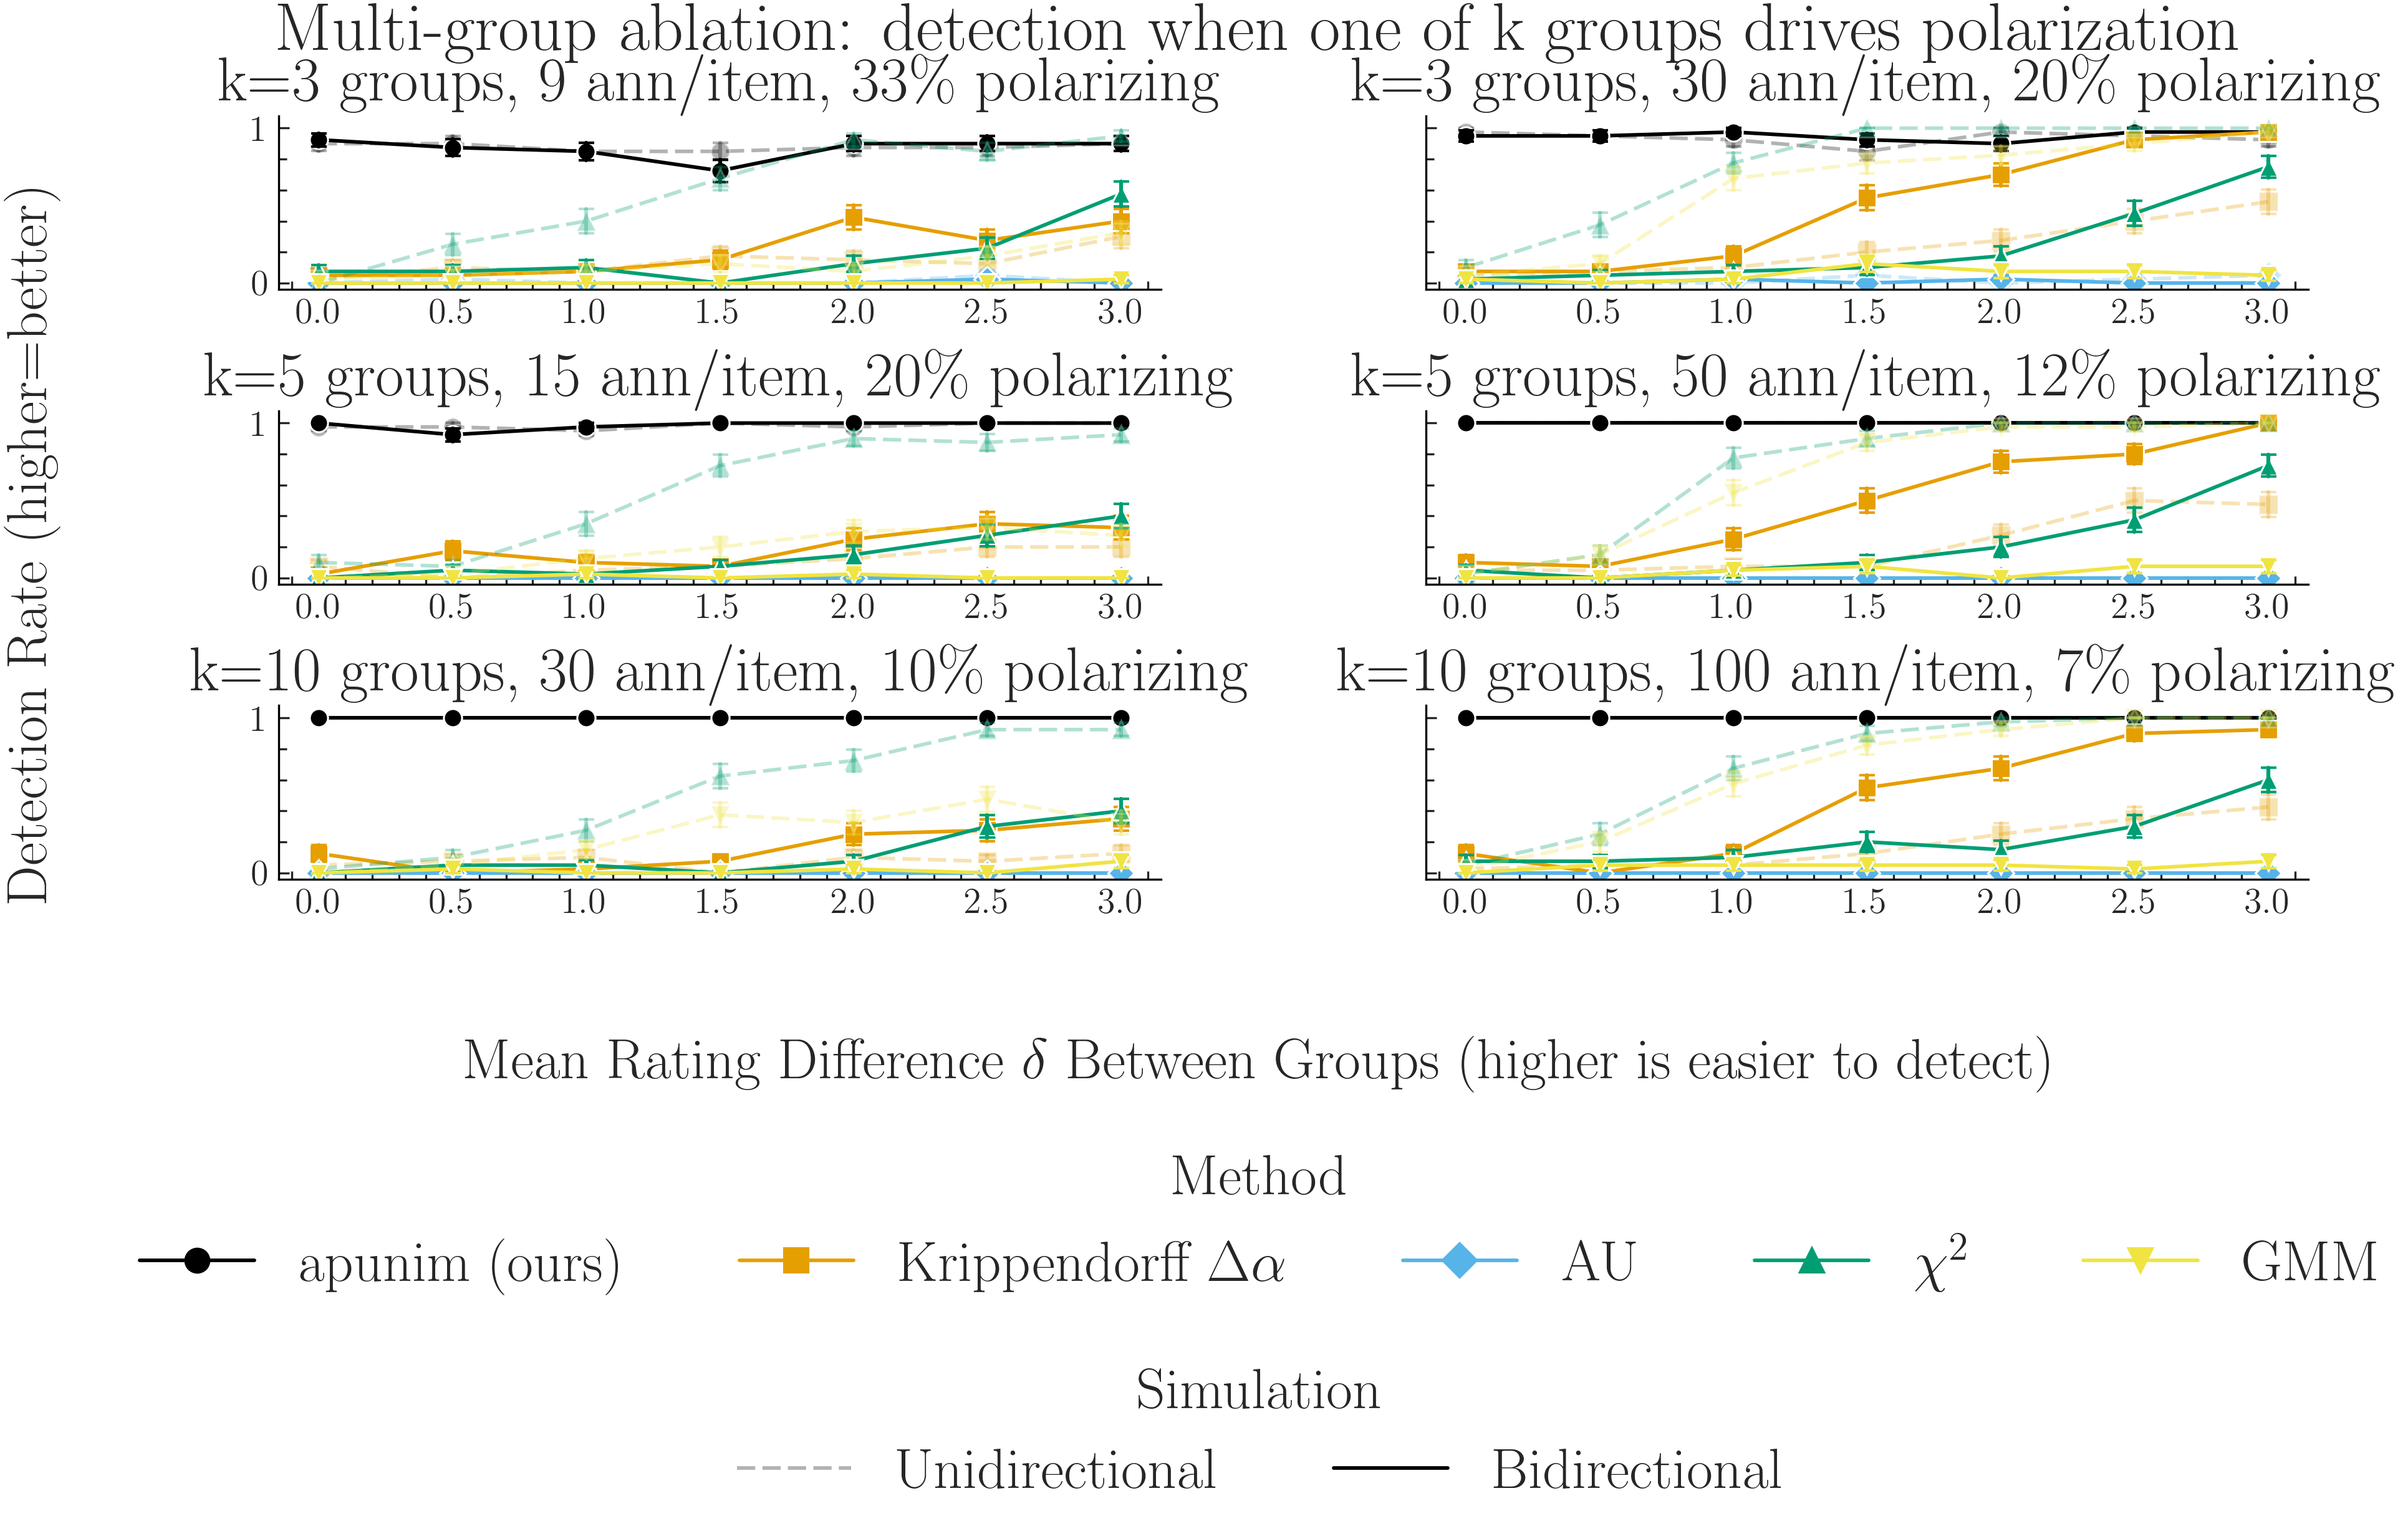
\includegraphics[width=\linewidth]{metric_comparison_multiple.png}
	\centering
	\caption{Polarization group attribution on synthetic distributions. Bars indicate standard error. The setup is identical to the one used for Fig.~\ref{fig:measures}, although in these experiments we consider multiple $k$ annotator groups for each item. Dashed lines show the results of a simplified polarization setup, where polarization always has the same direction.}
	\label{fig:measures-multiple}
\end{figure}

\paragraph{Does Apunim Work for More than Two Groups?} We repeat the experiment comparing apunim to prior methodologies shown in Fig.~\ref{fig:measures} but generalized across multiple groups. As shown in Fig.~\ref{fig:measures-multiple}, apunim stays competitive even in the presence of multiple annotator groups. Note the increased efficiency of many methods when polarization is unidirectional. This pattern indicates that the challenges of bidirectional polarization severely limiting prior approaches may be generalizable to more than two groups.

\begin{longtable}{llrrrr}
\caption{Comparison of Apunim values across different sample sizes (1k, 3k, 10k, 30k) for the Kumar dataset.} \label{tab:num-comments-apunim} \\
\toprule
 &  & \textbf{1000} & \textbf{3000} & \textbf{10000} & \textbf{30000} \\
 & \textbf{\ac{sdd}} &  &  &  &  \\
\midrule
\endfirsthead
\caption[]{Comparison of Apunim values across different sample sizes (1k, 3k, 10k, 30k) for the Kumar dataset.} \\
\toprule
 &  & \textbf{1000} & \textbf{3000} & \textbf{10000} & \textbf{30000} \\
 & \textbf{\ac{sdd}} &  &  &  &  \\
\midrule
\endhead
\midrule
\multicolumn{6}{r}{Continued on next page} \\
\midrule
\endfoot
\bottomrule
\endlastfoot
\multirow[t]{6}{*}{Age} & 1) 18 - 24 & 0.014 & -0.017 & -0.037 & -0.016 \\
 & 2) 25 - 34 & -0.003 & -0.000 & 0.000 & 0.000 \\
 & 3) 35 - 44 & 0.000 & -0.011 & -0.001 & -0.001 \\
 & 4) 45 - 54 & 0.022 & 0.033 & 0.013 & 0.003 \\
 & 5) 55 - 64 & 0.000 & 0.000 & -0.057 & 0.001 \\
 & 6) 65 or older & --- & --- & --- & 0.948 \\
\cline{1-6}
\multirow[t]{5}{*}{Education} & 2) High School graduate & 0.000 & 0.000 & -0.005 & 0.014 \\
 & 3) College, no degree & 0.010 & 0.014 & 0.010 & 0.006 \\
 & 4) Associate degree & 0.000 & 0.000 & 0.005 & 0.009 \\
 & 5) Bachelor's degree & 0.001 & -0.000 & -0.001 & -0.000 \\
 & 6) Master's degree & 0.000 & -0.006 & 0.004 & -0.000 \\
\cline{1-6}
\multirow[t]{6}{*}{Ethnicity} & Asian & -0.000 & 0.000 & 0.011 & 0.007 \\
 & Black & 0.000 & -0.024 & -0.004 & -0.012 \\
 & Hispanic & --- & --- & 0.000 & -0.099 \\
 & Multiracial & 0.000 & 0.000 & 0.000 & 0.000 \\
 & Other & --- & --- & --- & -0.306 \\
 & White & 0.000 & -0.000 & -0.000 & 0.000 \\
\cline{1-6}
\multirow[t]{2}{*}{Gender} & Female & 0.001 & 0.000 & 0.002 & 0.001 \\
 & Male & 0.001 & -0.004 & -0.002 & -0.001 \\
\cline{1-6}
\multirow[t]{2}{*}{Has Been Targeted} & False & 0.001 & 0.000 & -0.000 & 0.000 \\
 & True & -0.009 & -0.015 & -0.003 & -0.002 \\
\cline{1-6}
\multirow[t]{3}{*}{Is Parent} & No & -0.002 & 0.002 & 0.001 & 0.001 \\
 & Prefer not to say & --- & --- & 1.000 & 0.000 \\
 & Yes & -0.000 & 0.000 & -0.000 & 0.000 \\
\cline{1-6}
Is Transgender & No & 0.000 & 0.000 & 0.000 & 0.000 \\
\cline{1-6}
\multirow[t]{5}{*}{Political Affiliation} & Conservative & -0.013 & 0.003 & -0.003 & -0.002 \\
 & Independent & 0.000 & -0.001 & 0.001 & 0.002 \\
 & Liberal & -0.001 & 0.006 & 0.001 & 0.001 \\
 & Other & --- & 0.000 & 0.000 & 0.000 \\
 & Prefer not to say & --- & --- & 0.000 & 0.022 \\
\cline{1-6}
\multirow[t]{4}{*}{Religion Important} & 1) No & 0.002 & 0.004 & 0.002 & 0.001 \\
 & 2) Not very & 0.000 & -0.006 & 0.010 & 0.006 \\
 & 3) Somewhat & 0.000 & 0.002 & 0.003 & -0.002 \\
 & 4) Very & 0.000 & -0.003 & -0.003 & -0.002 \\
\cline{1-6}
\multirow[t]{2}{*}{Seen Toxicity} & False & -0.007 & 0.002 & -0.001 & -0.001 \\
 & True & -0.001 & 0.000 & 0.001 & 0.000 \\
\cline{1-6}
\multirow[t]{4}{*}{Sexual Orientation} & Bisexual & -0.068 & -0.029 & -0.040 & -0.013 \\
 & Heterosexual & -0.001 & -0.000 & -0.000 & 0.000 \\
 & Homosexual & --- & --- & 0.000 & 0.053 \\
 & Prefer not to say & --- & --- & --- & 0.370 \\
\cline{1-6}
\multirow[t]{4}{*}{Technology Impact} & 2) Somewhat negative & 0.000 & 0.000 & 0.000 & 0.003 \\
 & 3) Neutral & 0.124 & 0.037 & -0.014 & 0.000 \\
 & 4) Somewhat positive & 0.004 & 0.001 & -0.000 & 0.001 \\
 & 5) Very positive & -0.015 & -0.004 & -0.004 & -0.003 \\
\cline{1-6}
\multirow[t]{5}{*}{Toxicity Problem} & 1) Never & 0.000 & 0.000 & -0.037 & -0.081 \\
 & 2) Rarely & 0.000 & 0.000 & 0.003 & -0.001 \\
 & 3) Occasionally & 0.000 & -0.004 & -0.003 & -0.001 \\
 & 4) Frequently & 0.000 & 0.000 & -0.001 & -0.000 \\
 & 5) Very Frequently & 0.000 & -0.002 & 0.030 & 0.015 \\
\cline{1-6}
\end{longtable}


\begin{figure}[t]
	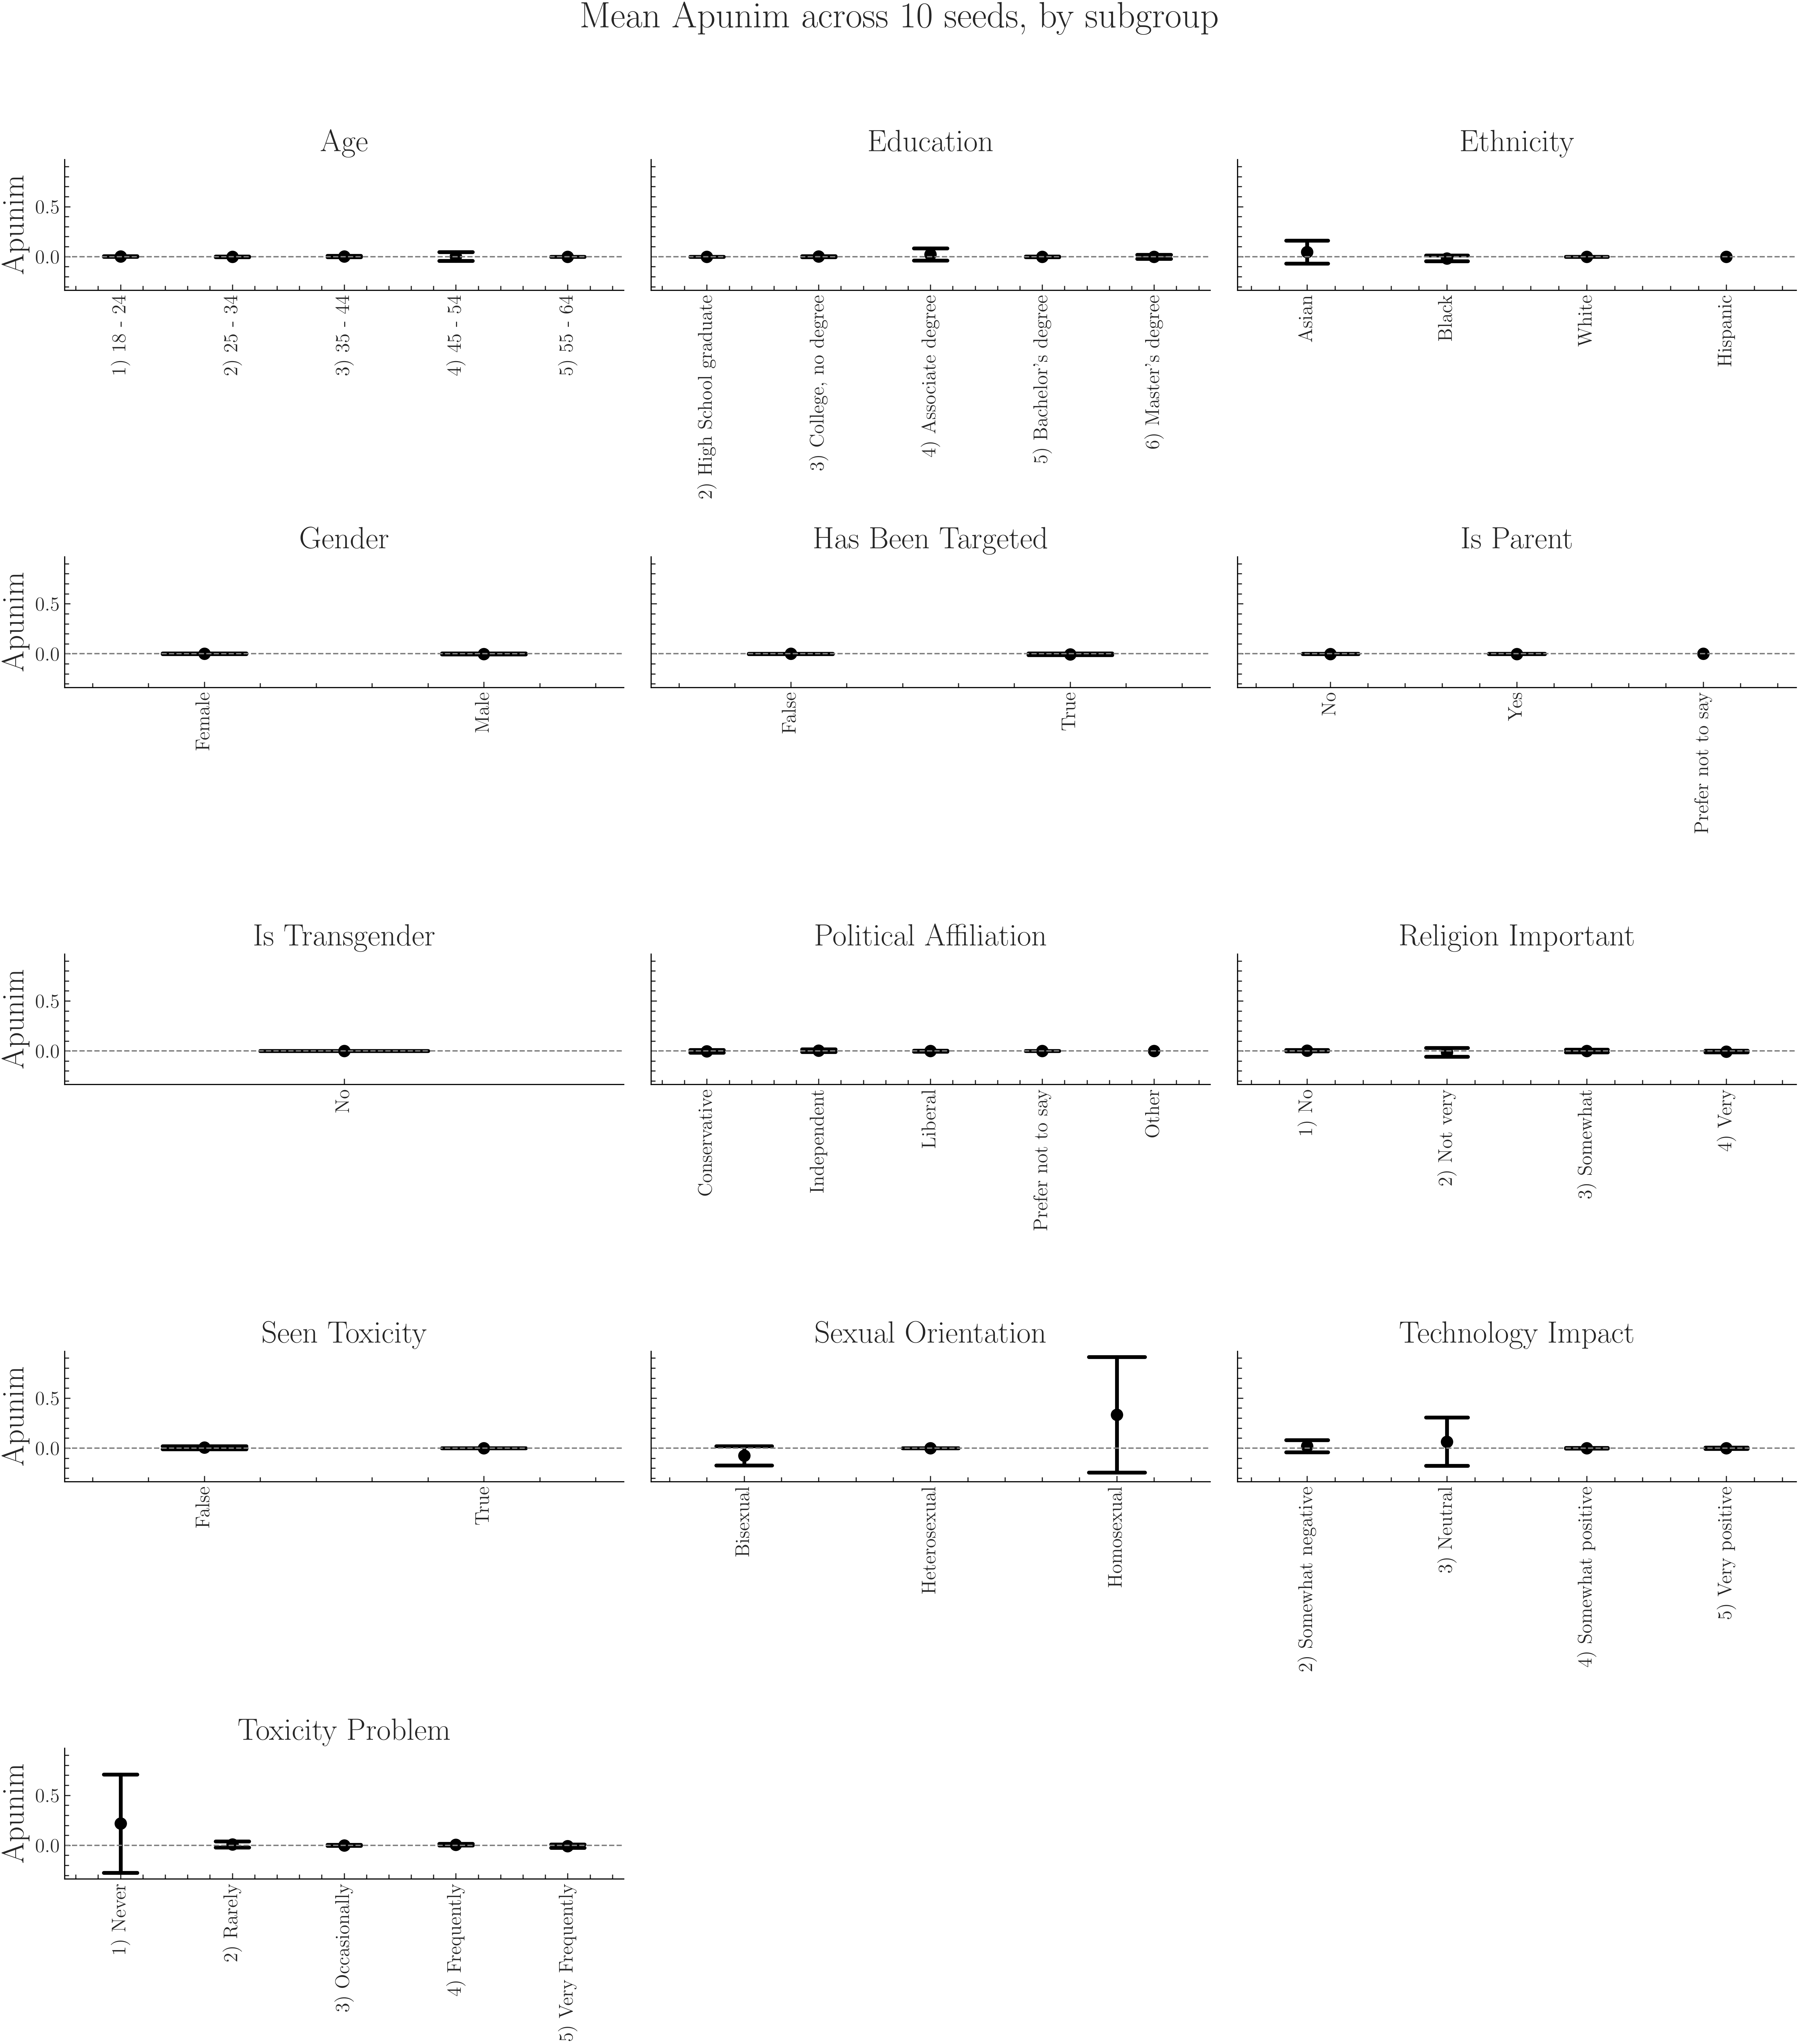
\includegraphics[width=\linewidth]{kumar1k_seed_ablation.png}
	\centering
	\caption{Apunim values on the Kumar dataset ($n_{samples}=1000$) across ten runs with different subsets.  Black bars indicate two \acp{sd}. \acp{sdd} with many groups are more volatile, although all \acp{sdd} broadly keep the same apunim sign across subsets.}
	\label{fig:seeds}
\end{figure}

\paragraph{How Does Dataset Size Influence Apunim?} Since our approach was designed for the small-scale datasets common in \ac{nlp}, we were cautious when testing it on the massive Kumar dataset. Because of the data volume, we analyzed various smaller samples (1{,}000, 3{,}000, 10{,}000, and 30{,}000 items), shown in Table~\ref{tab:num-comments-apunim}. Sample size does not seem to have a consistent effect on apunim values, other than large splits uncovering significant polarization effects in sparsely populated groups (e.g., 65+ yo. in \textit{Age}, ``Prefer Not to Say'' in \textit{Sexual Orientation}, ``Never'' , ``Very Frequently'' in \textit{Toxicity Problem}). The apunim direction stays broadly the same. We also test whether the results in Table~\ref{tab:apunim-main} are an artifact of the dataset split, because of the small sample size used in the study. We repeat the apunim experiment with ten different subsets of the same dataset and record their apunim values, shown in Fig.~\ref{fig:seeds}. We find that most apunim values are stable, save for ``Never'' in \textit{Toxicity Problem}, ``Heterosexual'' in \textit{Sexual Orientation} and ``Neutral'' in \textit{Technology Impact}.

\paragraph{How Does Sample Selection Influence Apunim?}
Astute readers may notice that some variability does exist across differently sized samples for the same examined groups, where for example the sign of the apunim value may switch. We note that the statistically significant values (bold rows) change signs only when the apunim value approaches zero in the largest samples. Thus, the results are not inverted, but rather pushed towards zero. In order to verify that this variability is caused by the sample size, and not by different samples being drawn, we execute a further ablation study. Specifically, we execute the apunim study on the $3000$-sized sample of the dataset, using different subsets of the Kumar dataset. The results can be found in Fig.~\ref{fig:seeds}, where we note that variability is not an issue, except for a couple of cases. These cases seem to represent sparse annotator groups, where missing a few items may genuinely change the value of the apunim measure. These groups however are largely not detected by apunim as significant either way (see Table~\ref{tab:apunim-main}).


\begin{figure}[t]
	\centering
	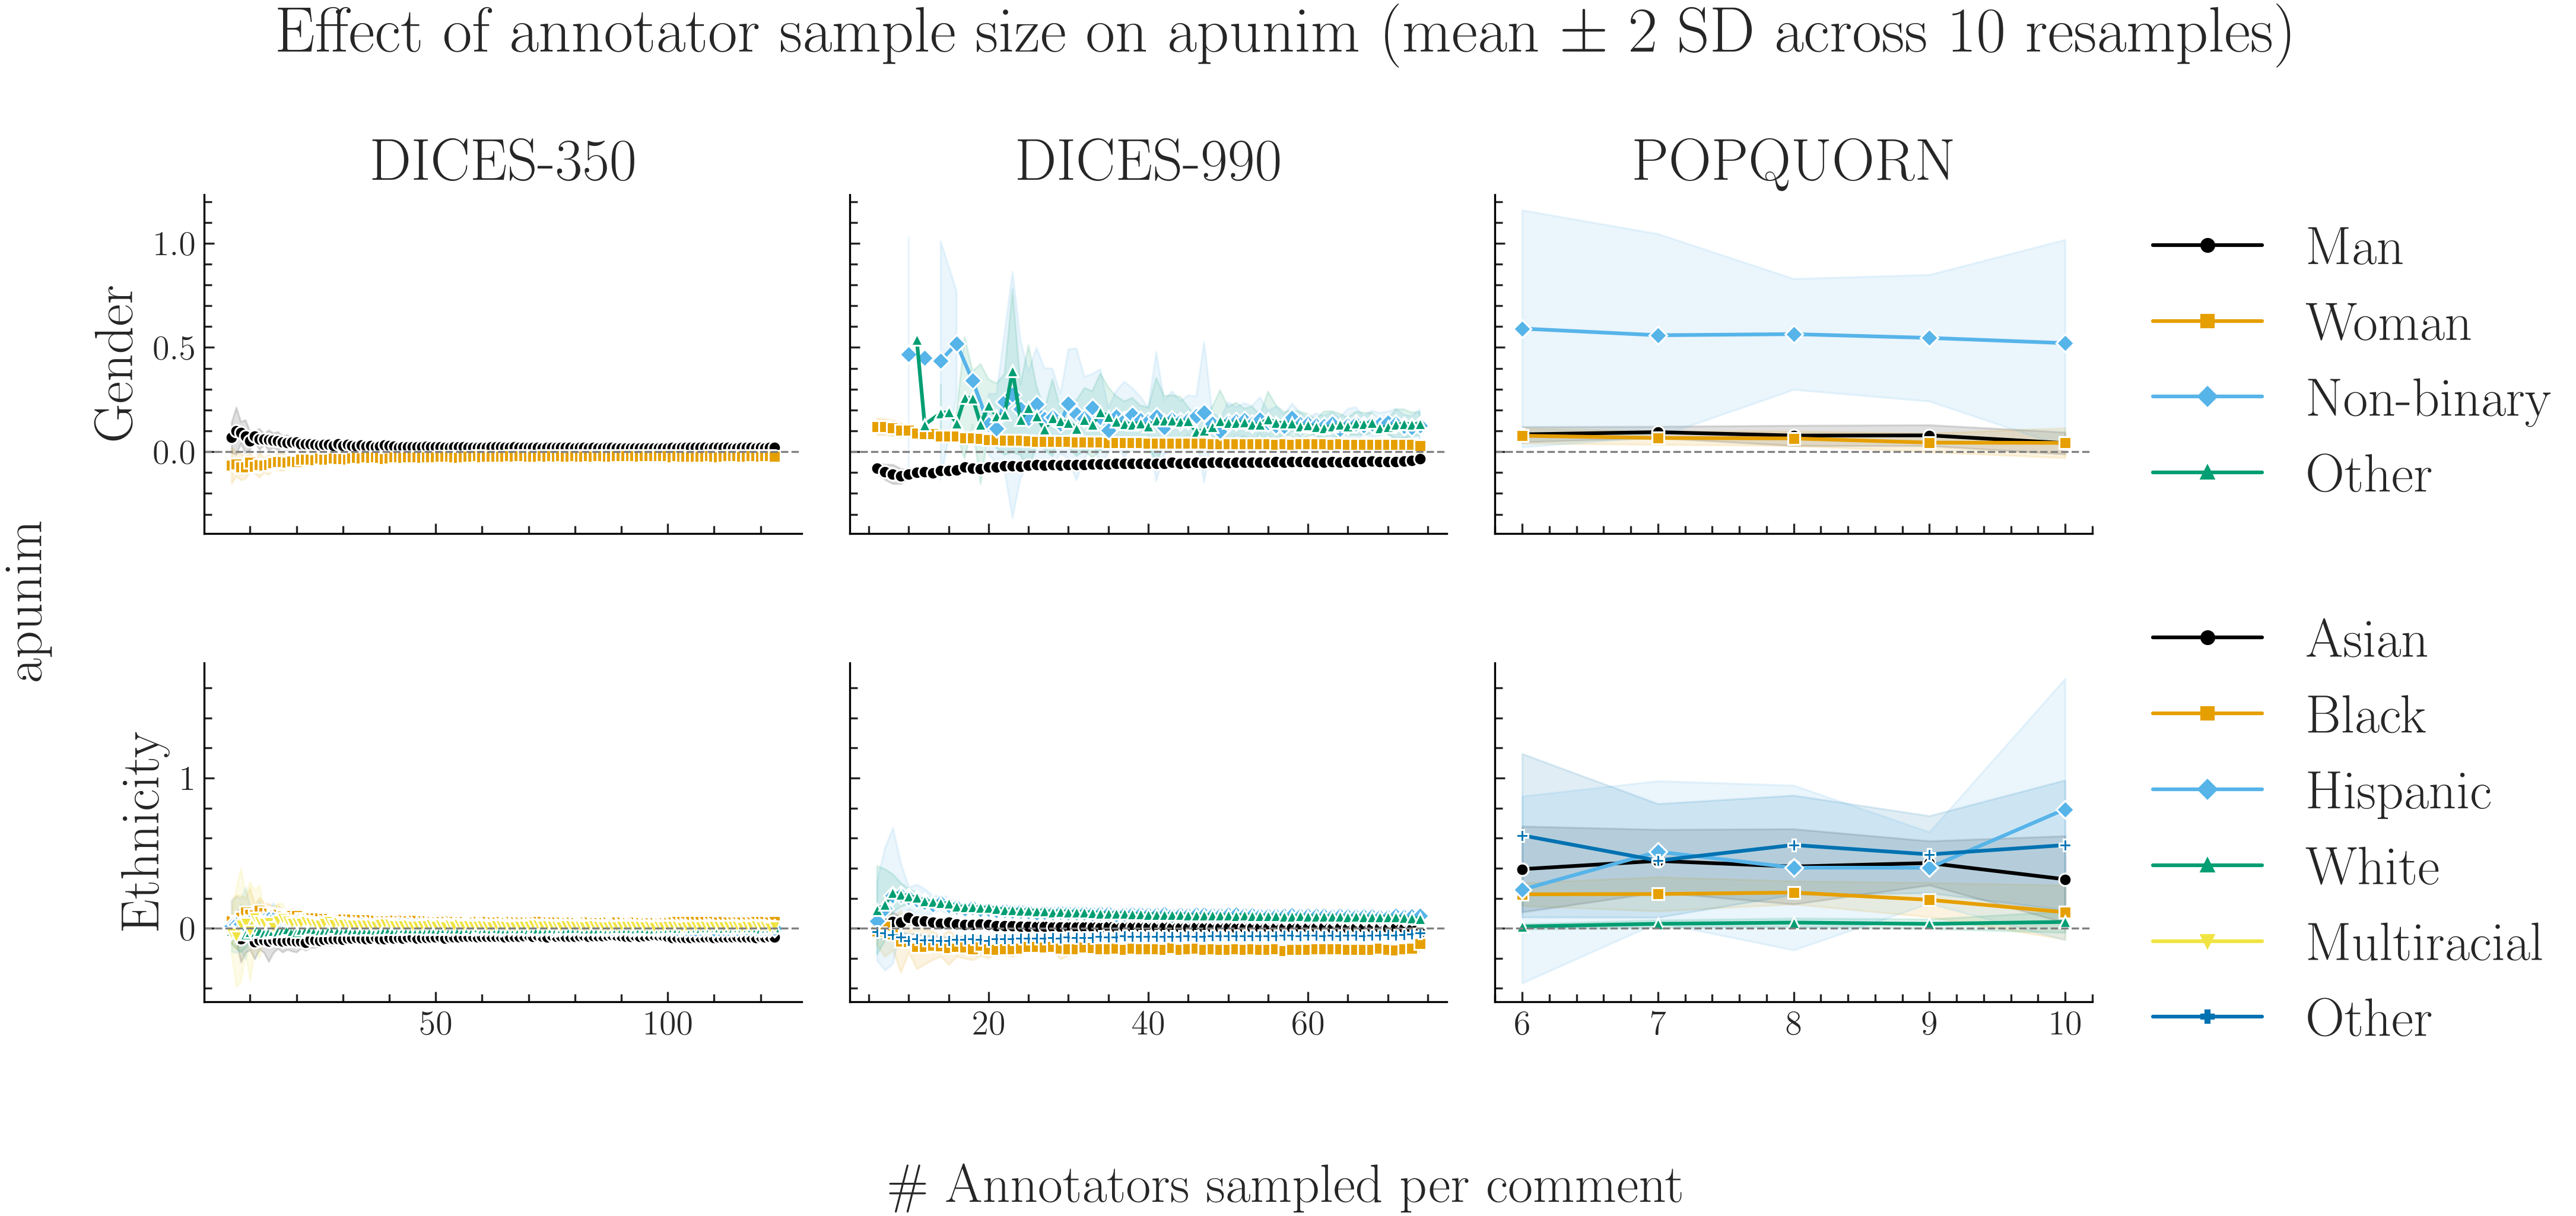
\includegraphics[width=\linewidth]{apunim_subsampling_robustness.png}
	\caption{\ac{sd} of $apunim$ across items, averaged across $10$ runs, where each item is resampled $100$ times. Shaded areas represent two \acp{sd}.}
	\label{fig:std_error}
\end{figure}

\paragraph{How Many Annotators Does Apunim Need?} Fig.~\ref{fig:std_error} sows that non-statistically significant results from Table~\ref{tab:apunim-main} remain systematically close to zero, while statistically significant results can be distinguished from very small annotator counts (six annotators for well-balanced groups, $\approx 20$ for poorly split groups such as non-binary annotators in DICES-990). Sampling annotators with replacement also uncovers a new group which systematically disagrees with the others; the Non-Binary annotators in the POPQUORN and DICES-990 datasets. This group was undetectable when partitioning annotator groups with the methodology described in Eq.~\ref{eq:apunim} since only one item is annotated by three \emph{Non-Binary} annotators in POPQUORN and none for DICES-990, but sampling with replacement uncovers a very strong attribution. It is unclear whether this is a methodological artifact, or a new finding unexplored in prior analysis concerning these datasets.

\section{LLM Annotation Procedure}
\label{app:llms}

\subsection{Models Used}

We use only open-source models, as proprietary models such as OpenAI's GPT-5 yield much less reproducible results~\citep{bisbee_2023}. Furthermore, the use of open-source models requires much fewer resources, enabling research on this task with a less demanding budget, as well as scalable deployment in real-world settings~\citep{rossi_2024}. It is also worth noting that since the datasets used are not publicly licensed, we can not risk leaking the data contained within to proprietary models. Generally, the use of local models protects the personal data of the users contained in our datasets, ensures that our research can be replicated in domains where anonymity must be maintained, and renders our work compatible with existing legislation~\citep{eu_ai_act, GDPR}. Table~\ref{tab:llm-details} shows details on the LLMs used for this study. We specifically use 4-bit quantized versions from the \texttt{unsloth huggingface} repository.

\begin{table}[ht]
	\caption{LLMs used in this study.}
	\label{tab:llm-details}
	\centering
	\begin{tabular}{l l l l}
		\toprule
		\textbf{Family} & \textbf{Version} & \textbf{\#Params} & \textbf{Year} \\
		\midrule
		\texttt{OLMo}~\citep{groeneveld-etal-2024-olmo} & \texttt{2 (0325)} & 32B & 2025 \\
		\texttt{Qwen}~\citep{qwen2025qwen25technicalreport} & \texttt{2.5} & 32B & 2024 \\
		\texttt{OLMo}~\citep{olmo2026olmo3} & \texttt{3} & 7B & 2025 \\
		\texttt{Qwen}~\citep{qwen2025qwen25technicalreport} & \texttt{2.5} & 7B & 2024 \\
		\texttt{LLaMa}~\citep{grattafiori2024llama3herdmodels} & \texttt{3.1} & 8B & 2024 \\
		\texttt{Mistral}~\citep{jiang2023mistral7b} & \texttt{Small 3 (2501)} & 24B & 2025 \\
		\texttt{Mistral}~\citep{jiang2023mistral7b} & \texttt{v0.3} & 7B & 2024 \\
		\texttt{Gemma}~\citep{gemma4} & \texttt{4} & E2B & 2026 \\
		\texttt{Gemma}~\citep{gemma4} & \texttt{4} & 31B & 2026 \\
		\bottomrule
	\end{tabular}
\end{table}

\subsection{Experimental Setup}
Since each of the datasets in \S\ref{sec:datasets} was annotated using different annotation guidelines and targets we use different instruction prompts for each dataset. The ``default'' annotation prompt is directly extracted from the studies in the case of Sap and Kumar, and inferred from the instruction guidelines used in the DICES datasets with minor modifications. We use standard persona prompting procedures sampled randomly from the available \acp{sdd} in each respective dataset. Twenty LLM annotators are selected for each item and model.

The prompts used in the ablation study were provided by a GPT-5 and a local Gemma-4 (quantized) model by providing the original prompt and instructing it to produce four variants. The tested prompts use different methods to restrict the model's behavior. The initial prompts  (``\textit{Persona}''require the model to adopt a persona's viewpoint to judge the comment. Other prompts (``\textit{direct}'') treat the persona's characteristics as an absolute, non-negotiable rule that overrides standard moderation guidelines. Another approach (``single'') compels the model to perform a persona-based check before submitting its final rating. The most aggressive prompts (``stereotype'') force the model into extreme decision spaces. The full main and ablation annotation prompts can be found in App.~\ref{app:prompts}. 

We use a single Quadro RTX 6000 GPU for tasks requiring small (7-8B) models and two such GPUs for the rest. The annotation task, including ablations, requires approximately 300 hours of computation to complete. We use the \texttt{transformers} library to load and manage the LLMs. We release the relevant code in the supplementary material. Our codebase is platform-independent except for three high-level bash scripts and a full environment file is included for reproduction.


\subsection{Exploratory Analysis}

%TODO: Fix the figure and place other graphs here
\begin{figure*}[t]
	\centering
	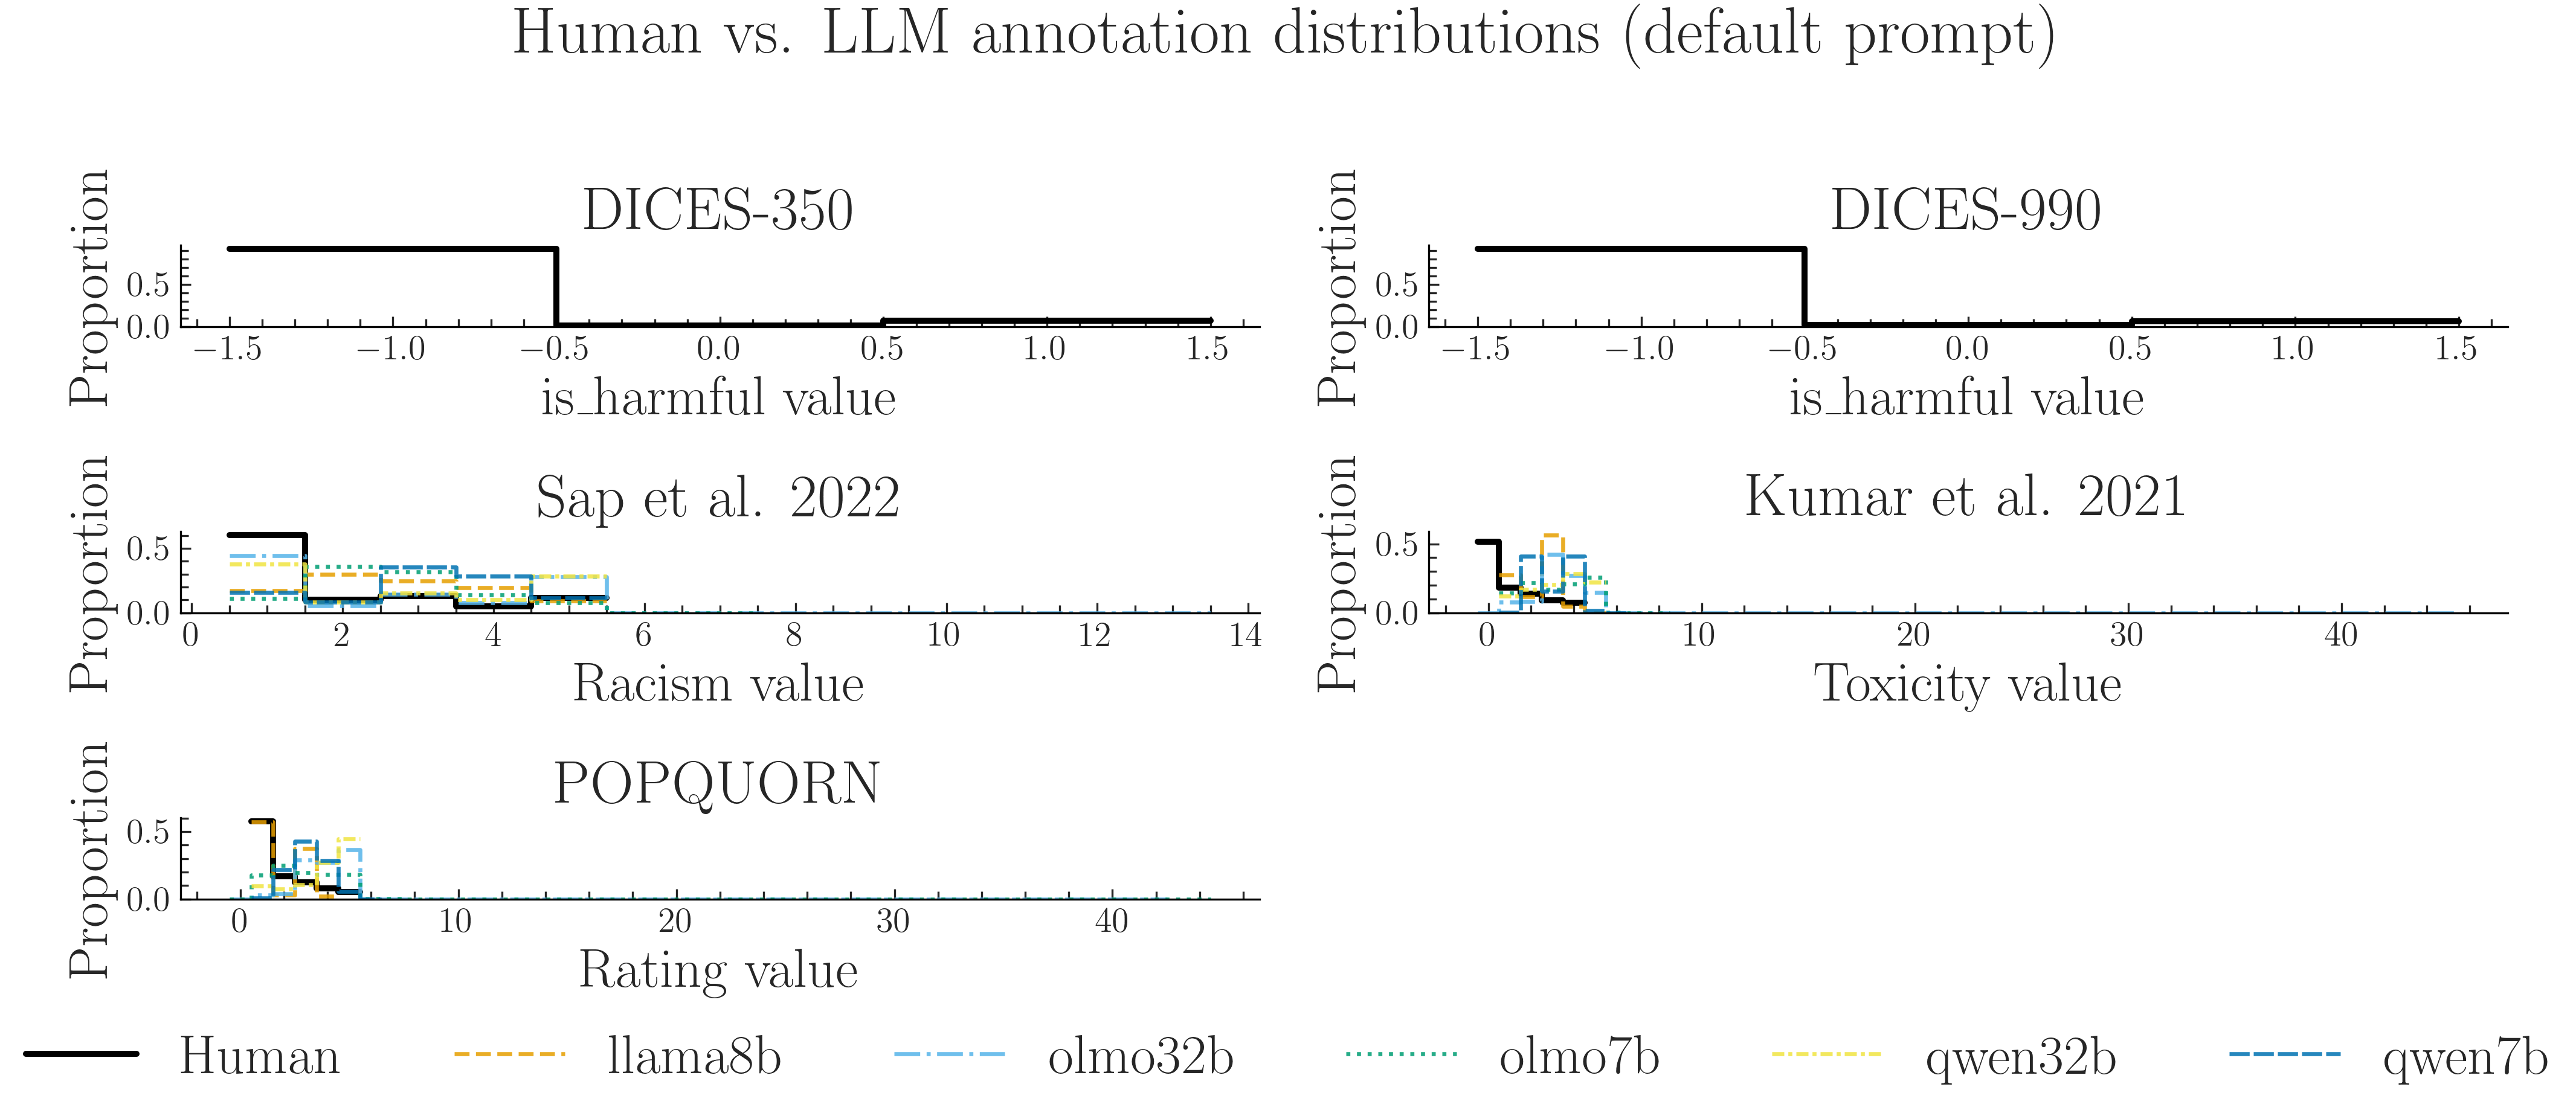
\includegraphics[width=\linewidth]{human_vs_llm_histograms.png}
	\caption{Annotation frequencies for humans and each LLM in the primary annotation task using the default prompt.}
	\label{fig:llm-human-frequencies}
\end{figure*}

\paragraph{Frequencies} Fig.~\ref{fig:llm-human-frequencies} shows the different annotation frequencies of LLMs and human annotators in the same dataset split. Across all datasets, we observe a consistent mismatch between human and LLM annotation distributions. For the DICES-350 and DICES-990 harmfulness tasks, human annotations are heavily concentrated at the lowest harmfulness value, whereas most LLMs assign substantially more probability to moderate and high harmfulness values. A similar pattern appears in the \citet{sap-etal-2022-annotators} racism dataset: human judgments are concentrated at low racism scores, while LLMs produce broader distributions with considerably more mass at higher scores, particularly values 4--5. The \citep{kumar-et-al-2021} toxicity results show the same general trend, with humans assigning most probability to zero toxicity while LLMs distribute their predictions across higher toxicity levels, often peaking around values 2--4. Importantly, the magnitude of this discrepancy varies across models; some LLMs are closer to the human distribution, while others show substantially stronger shifts toward higher scores.

\begin{table}[htbp]
\small
\centering
\caption{Number of non-standard LLM annotations per model and dataset, summed over all instruction prompts. Unparsed: no integer found in the reply (dropped from the analysis); Out of range: an integer outside the dataset's annotation scale. Incidence: percentage of the model's annotations on that dataset.}
\label{tab:nonstandard-answers}
\begin{tabular}{lllrl}
\toprule
Model & Dataset & Status & Count & Incidence (\%) \\
\midrule
Gemma 31B & POPQUORN & Unparsed & 104 & 0.09 \\
Gemma 31B & Sap & Unparsed & 8 & 0.01 \\
Gemma 5B & Kumar & Unparsed & 12 & 0.01 \\
Gemma 5B & POPQUORN & Out of range & 1 & 0.00 \\
Gemma 5B & POPQUORN & Unparsed & 340 & 0.23 \\
Gemma 5B & Sap & Out of range & 20 & 0.03 \\
Gemma 5B & Sap & Unparsed & 2 & 0.00 \\
Llama 8B & Kumar & Out of range & 153 & 0.15 \\
Llama 8B & Kumar & Unparsed & 33352 & 33.35 \\
Llama 8B & POPQUORN & Out of range & 1 & 0.00 \\
Llama 8B & POPQUORN & Unparsed & 47661 & 31.77 \\
Llama 8B & Sap & Unparsed & 20552 & 35.13 \\
Mistral 24B & Kumar & Out of range & 1 & 0.00 \\
Mistral 24B & Kumar & Unparsed & 14745 & 14.74 \\
Mistral 24B & POPQUORN & Unparsed & 28599 & 19.07 \\
Mistral 24B & Sap & Unparsed & 16783 & 28.69 \\
Mistral 7B & Kumar & Out of range & 5 & 0.01 \\
Mistral 7B & Kumar & Unparsed & 12152 & 12.15 \\
Mistral 7B & POPQUORN & Out of range & 62 & 0.04 \\
Mistral 7B & POPQUORN & Unparsed & 6174 & 4.12 \\
Mistral 7B & Sap & Unparsed & 2771 & 4.74 \\
OLMo 32B & Kumar & Out of range & 25 & 0.03 \\
OLMo 32B & Kumar & Unparsed & 270 & 0.27 \\
OLMo 32B & POPQUORN & Out of range & 10 & 0.01 \\
OLMo 32B & POPQUORN & Unparsed & 1504 & 1.00 \\
OLMo 32B & Sap & Out of range & 2 & 0.00 \\
OLMo 32B & Sap & Unparsed & 953 & 1.63 \\
OLMo 7B & Kumar & Out of range & 96 & 0.10 \\
OLMo 7B & Kumar & Unparsed & 613 & 0.61 \\
OLMo 7B & POPQUORN & Out of range & 110 & 0.07 \\
OLMo 7B & POPQUORN & Unparsed & 4849 & 3.23 \\
OLMo 7B & Sap & Out of range & 37 & 0.06 \\
OLMo 7B & Sap & Unparsed & 3867 & 6.61 \\
Qwen 32B & Kumar & Unparsed & 1 & 0.00 \\
Qwen 7B & Kumar & Out of range & 137 & 0.14 \\
Qwen 7B & Kumar & Unparsed & 22 & 0.02 \\
Qwen 7B & POPQUORN & Unparsed & 42 & 0.03 \\
Qwen 7B & Sap & Unparsed & 5 & 0.01 \\
\bottomrule
\end{tabular}
\end{table}


\paragraph{Dropped Responses} Table~\ref{tab:nonstandard-answers} shows a breakdown of failure modes across models and datasets. Most failed answers stem from the model refusing to provide any number in their response. Some attempt to initiate a Chain of Thought response, which is truncated due to us forcing a three-token limit on LLM answers. Others refuse to respond due to safety tuning. Finally, some (and especially the smaller Gemma model) seem to produce degenerate integer outputs. The full file of failed responses can be found in the Supplementary Material.


\subsection{Annotation Ablations}

\begin{center}
	\begin{table}[t]
\centering
\caption{Consistency (Krippendorff's $\alpha$, ordinal) of each model with itself across repeated runs of the same (default) prompt.}
\label{tab:llm-consistency-repeats}
\begin{tabular}{llrrl}
\toprule
Dataset & Model & Runs & Items & Krippendorff's alpha \\
\midrule
DICES-350 & Gemma 31B & 5 & 210 & 1.0000 \\
DICES-350 & Gemma 5B & 5 & 210 & 1.0000 \\
DICES-350 & Llama 8B & 5 & 210 & 1.0000 \\
DICES-350 & Mistral 24B & 5 & 210 & 1.0000 \\
DICES-350 & Mistral 7B & 5 & 210 & 1.0000 \\
DICES-350 & OLMo 32B & 5 & 209 & 1.0000 \\
DICES-350 & OLMo 7B & 5 & 210 & 1.0000 \\
DICES-350 & Qwen 32B & 5 & 210 & 1.0000 \\
DICES-350 & Qwen 7B & 5 & 210 & 1.0000 \\
DICES-990 & Gemma 31B & 5 & 594 & --- \\
DICES-990 & Gemma 5B & 5 & 594 & 1.0000 \\
DICES-990 & Llama 8B & 5 & 594 & 1.0000 \\
DICES-990 & Mistral 24B & 5 & 592 & 1.0000 \\
DICES-990 & Mistral 7B & 5 & 594 & --- \\
DICES-990 & OLMo 32B & 5 & 594 & 1.0000 \\
DICES-990 & OLMo 7B & 5 & 594 & 1.0000 \\
DICES-990 & Qwen 32B & 5 & 594 & 1.0000 \\
DICES-990 & Qwen 7B & 5 & 594 & 1.0000 \\
Sap & Gemma 31B & 5 & 348 & 1.0000 \\
Sap & Gemma 5B & 5 & 348 & 1.0000 \\
Sap & Llama 8B & 5 & 287 & 1.0000 \\
Sap & Mistral 24B & 5 & 348 & 1.0000 \\
Sap & Mistral 7B & 5 & 345 & 1.0000 \\
Sap & OLMo 32B & 5 & 343 & 1.0000 \\
Sap & OLMo 7B & 5 & 338 & 1.0000 \\
Sap & Qwen 32B & 5 & 348 & 1.0000 \\
Sap & Qwen 7B & 5 & 348 & 1.0000 \\
Kumar & Gemma 31B & 5 & 600 & 1.0000 \\
Kumar & Gemma 5B & 5 & 600 & 1.0000 \\
Kumar & Llama 8B & 5 & 458 & 1.0000 \\
Kumar & Mistral 24B & 5 & 600 & 1.0000 \\
Kumar & Mistral 7B & 5 & 597 & 1.0000 \\
Kumar & OLMo 32B & 5 & 599 & 1.0000 \\
Kumar & OLMo 7B & 5 & 600 & 1.0000 \\
Kumar & Qwen 32B & 5 & 600 & 1.0000 \\
Kumar & Qwen 7B & 5 & 600 & 1.0000 \\
POPQUORN & Gemma 5B & 5 & 900 & 1.0000 \\
POPQUORN & Llama 8B & 5 & 771 & 1.0000 \\
POPQUORN & Mistral 24B & 5 & 900 & 1.0000 \\
POPQUORN & Mistral 7B & 5 & 899 & 1.0000 \\
POPQUORN & OLMo 32B & 5 & 893 & 1.0000 \\
POPQUORN & OLMo 7B & 5 & 880 & 1.0000 \\
POPQUORN & Qwen 32B & 5 & 900 & 1.0000 \\
POPQUORN & Qwen 7B & 5 & 900 & 1.0000 \\
\bottomrule
\end{tabular}
\end{table}

	
	\begin{table}[t]
\centering
\caption{Consistency (Krippendorff's $\alpha$, ordinal) of each model with itself across the three paraphrased prompt variants.}
\label{tab:llm-consistency-variants}
\begin{tabular}{llrrl}
\toprule
Dataset & Model & Variants & Items & Krippendorff's alpha \\
\midrule
DICES-350 & Gemma 31B & 3 & 210 & 0.3361 \\
DICES-350 & Gemma 5B & 3 & 210 & -0.0473 \\
DICES-350 & Llama 8B & 3 & 210 & 0.0372 \\
DICES-350 & Mistral 24B & 3 & 210 & -0.3299 \\
DICES-350 & Mistral 7B & 3 & 210 & -0.0334 \\
DICES-350 & OLMo 32B & 3 & 210 & 0.0253 \\
DICES-350 & OLMo 7B & 3 & 210 & 0.1701 \\
DICES-350 & Qwen 32B & 3 & 210 & 0.0044 \\
DICES-350 & Qwen 7B & 3 & 210 & -0.2016 \\
DICES-990 & Gemma 31B & 3 & 594 & -0.0085 \\
DICES-990 & Gemma 5B & 3 & 594 & 0.7115 \\
DICES-990 & Llama 8B & 3 & 594 & -0.0310 \\
DICES-990 & Mistral 24B & 3 & 594 & -0.0829 \\
DICES-990 & Mistral 7B & 3 & 594 & -0.2069 \\
DICES-990 & OLMo 32B & 3 & 594 & 0.2378 \\
DICES-990 & OLMo 7B & 3 & 594 & 0.0594 \\
DICES-990 & Qwen 32B & 3 & 594 & 0.1905 \\
DICES-990 & Qwen 7B & 3 & 594 & 0.1101 \\
Sap & Gemma 31B & 3 & 348 & 0.9560 \\
Sap & Gemma 5B & 3 & 348 & 0.8905 \\
Sap & Llama 8B & 3 & 336 & 0.3863 \\
Sap & Mistral 24B & 3 & 348 & 0.7528 \\
Sap & Mistral 7B & 3 & 348 & 0.8446 \\
Sap & OLMo 32B & 3 & 347 & 0.8579 \\
Sap & OLMo 7B & 3 & 348 & 0.3025 \\
Sap & Qwen 32B & 3 & 348 & 0.9732 \\
Sap & Qwen 7B & 3 & 348 & 0.8625 \\
Kumar & Gemma 31B & 3 & 600 & 0.9258 \\
Kumar & Gemma 5B & 3 & 600 & 0.7871 \\
Kumar & Llama 8B & 3 & 594 & 0.0667 \\
Kumar & Mistral 24B & 3 & 600 & 0.8201 \\
Kumar & Mistral 7B & 3 & 599 & 0.6077 \\
Kumar & OLMo 32B & 3 & 600 & 0.5169 \\
Kumar & OLMo 7B & 3 & 600 & 0.0547 \\
Kumar & Qwen 32B & 3 & 600 & 0.9003 \\
Kumar & Qwen 7B & 3 & 600 & 0.2496 \\
POPQUORN & Gemma 31B & 3 & 900 & 0.8348 \\
POPQUORN & Gemma 5B & 3 & 900 & 0.8041 \\
POPQUORN & Llama 8B & 3 & 885 & 0.0175 \\
POPQUORN & Mistral 24B & 3 & 900 & 0.7000 \\
POPQUORN & Mistral 7B & 3 & 900 & 0.4874 \\
POPQUORN & OLMo 32B & 3 & 900 & 0.5657 \\
POPQUORN & OLMo 7B & 3 & 900 & 0.1038 \\
POPQUORN & Qwen 32B & 3 & 900 & 0.8381 \\
POPQUORN & Qwen 7B & 3 & 900 & 0.2747 \\
\bottomrule
\end{tabular}
\end{table}

	
	\begin{table}[t]
\centering
\caption{Consistency (Krippendorff's $\alpha$, ordinal) between LLMs given the same (default) prompt, per dataset.}
\label{tab:llm-consistency-cross-model}
\begin{tabular}{llrrl}
\toprule
Dataset & Prompt & Models & Items & Krippendorff's alpha \\
\midrule
Sap & default & 9 & 18230 & 0.5201 \\
Kumar & default & 9 & 40000 & 0.2035 \\
POPQUORN & default & 8 & 30000 & 0.2627 \\
\bottomrule
\end{tabular}
\end{table}

	
	\begin{table}[t]
\centering
\caption{Consistency (Krippendorff's $\alpha$, ordinal) between LLMs given the same (default) prompt, per dataset, excluding the following models: Llama 8B, OLMo 7B, Qwen 7B.}
\label{tab:llm-consistency-cross-model-excluding}
\begin{tabular}{llrrl}
\toprule
Dataset & Prompt & Models & Items & Krippendorff's alpha \\
\midrule
Sap & default & 6 & 18230 & 0.6465 \\
Kumar & default & 6 & 40000 & 0.3581 \\
POPQUORN & default & 5 & 30000 & 0.4213 \\
\bottomrule
\end{tabular}
\end{table}

	
	\begin{table}[t]
\small
\centering
\caption{Correlation between the per-comment \ac{ndfu} of the human annotations and the polarization ratings, per dataset. $n$ is the number of comments with both an \ac{ndfu} and a rating.}
\label{tab:human-ndfu-rating-correlations}
\begin{tabular}{lrrr}
\toprule
Dataset & $n$ & Spearman $\rho$ & Kendall $\tau_b$ \\
\midrule
POPQUORN & 1500 & 0.35 & 0.27 \\
Sap et al. 2022 & 585 & 0.06 & 0.05 \\
DICES-990 & 990 & 0.43 & 0.34 \\
DICES-350 & 350 & 0.33 & 0.26 \\
\bottomrule
\end{tabular}
\end{table}

\end{center}

We examine the following conditions for selecting models and datasets for our LLM annotation experiment. All ablation experiments use a sampled 20\% fraction of the full LLM annotation dataset used in the main text.

\paragraph{The LLMs should be consistent given the same prompt} While we have fixed all relevant seeds, it is possible that generation deviates across repeated model prompting given the same input \citep{bisbee_2023}. We check this condition by providing the model with the main annotation prompt (see App.~\ref{app:prompts}) five times and find that generation is indeed deterministic under our setup for all models (Table~\ref{tab:llm-consistency-repeats}).

\paragraph{The LLMs should be prompt insensitive} Small changes in the prompt have been shown to drastically affect LLM output in some tasks depending on the experimental setup \citep{razavi_sensitivity}. In order to verify whether any models are unreliable under our setup, we create two alternative formulations of each prompt without a change in substance using a GPT-5 model (free version), whose outputs we manually verified (see App.~\ref{app:prompts}). Table~\ref{tab:llm-consistency-variants} shows that while most LLMs are relatively robust to changes in formulation, the smaller ones (OLMo-7B, Qwen-7B and LLaMa-8B) are not. They are thus excluded from the annotation study.

\paragraph{The annotation guidelines should be unambiguous} The studies that provided the datasets used in our work (see \S\ref{sec:datasets}) do not include LLM annotation, nor equivalent LLM prompts, which meant we had to generate them from the human annotation guidelines ourselves. This was not a problem in the case of the Sap and Kumar datasets, since the annotation guidelines were short, simple and required minimal edits to be transformed into LLM annotation guidelines. However, the DICES datasets use poorly documented guidelines and the target label we used is an aggregation of multiple annotation tasks. For these reasons the prompt creation is non-trivial and prone to errors. Indeed, Table~\ref{tab:llm-consistency-cross-model} shows that inter-model agreement is extremely low for the DICES datasets, even when we remove the sensitive models (Table~\ref{tab:llm-consistency-cross-model-excluding}). Given that the DICES datasets are (1) problematic w.r.t. inherent polarization (see App.~\ref{app:unpol}), (2) conditioned on several dozen annotations per item (3) difficult to find reliable annotation prompts for LLMs, we decided to exclude them from the annotation study.

\paragraph{Can we Infer Polarization Using Text?} Table~\ref{tab:ndfu-rating-correlations}




\subsection{LLM Annotation Results}

\begin{figure}[t]
	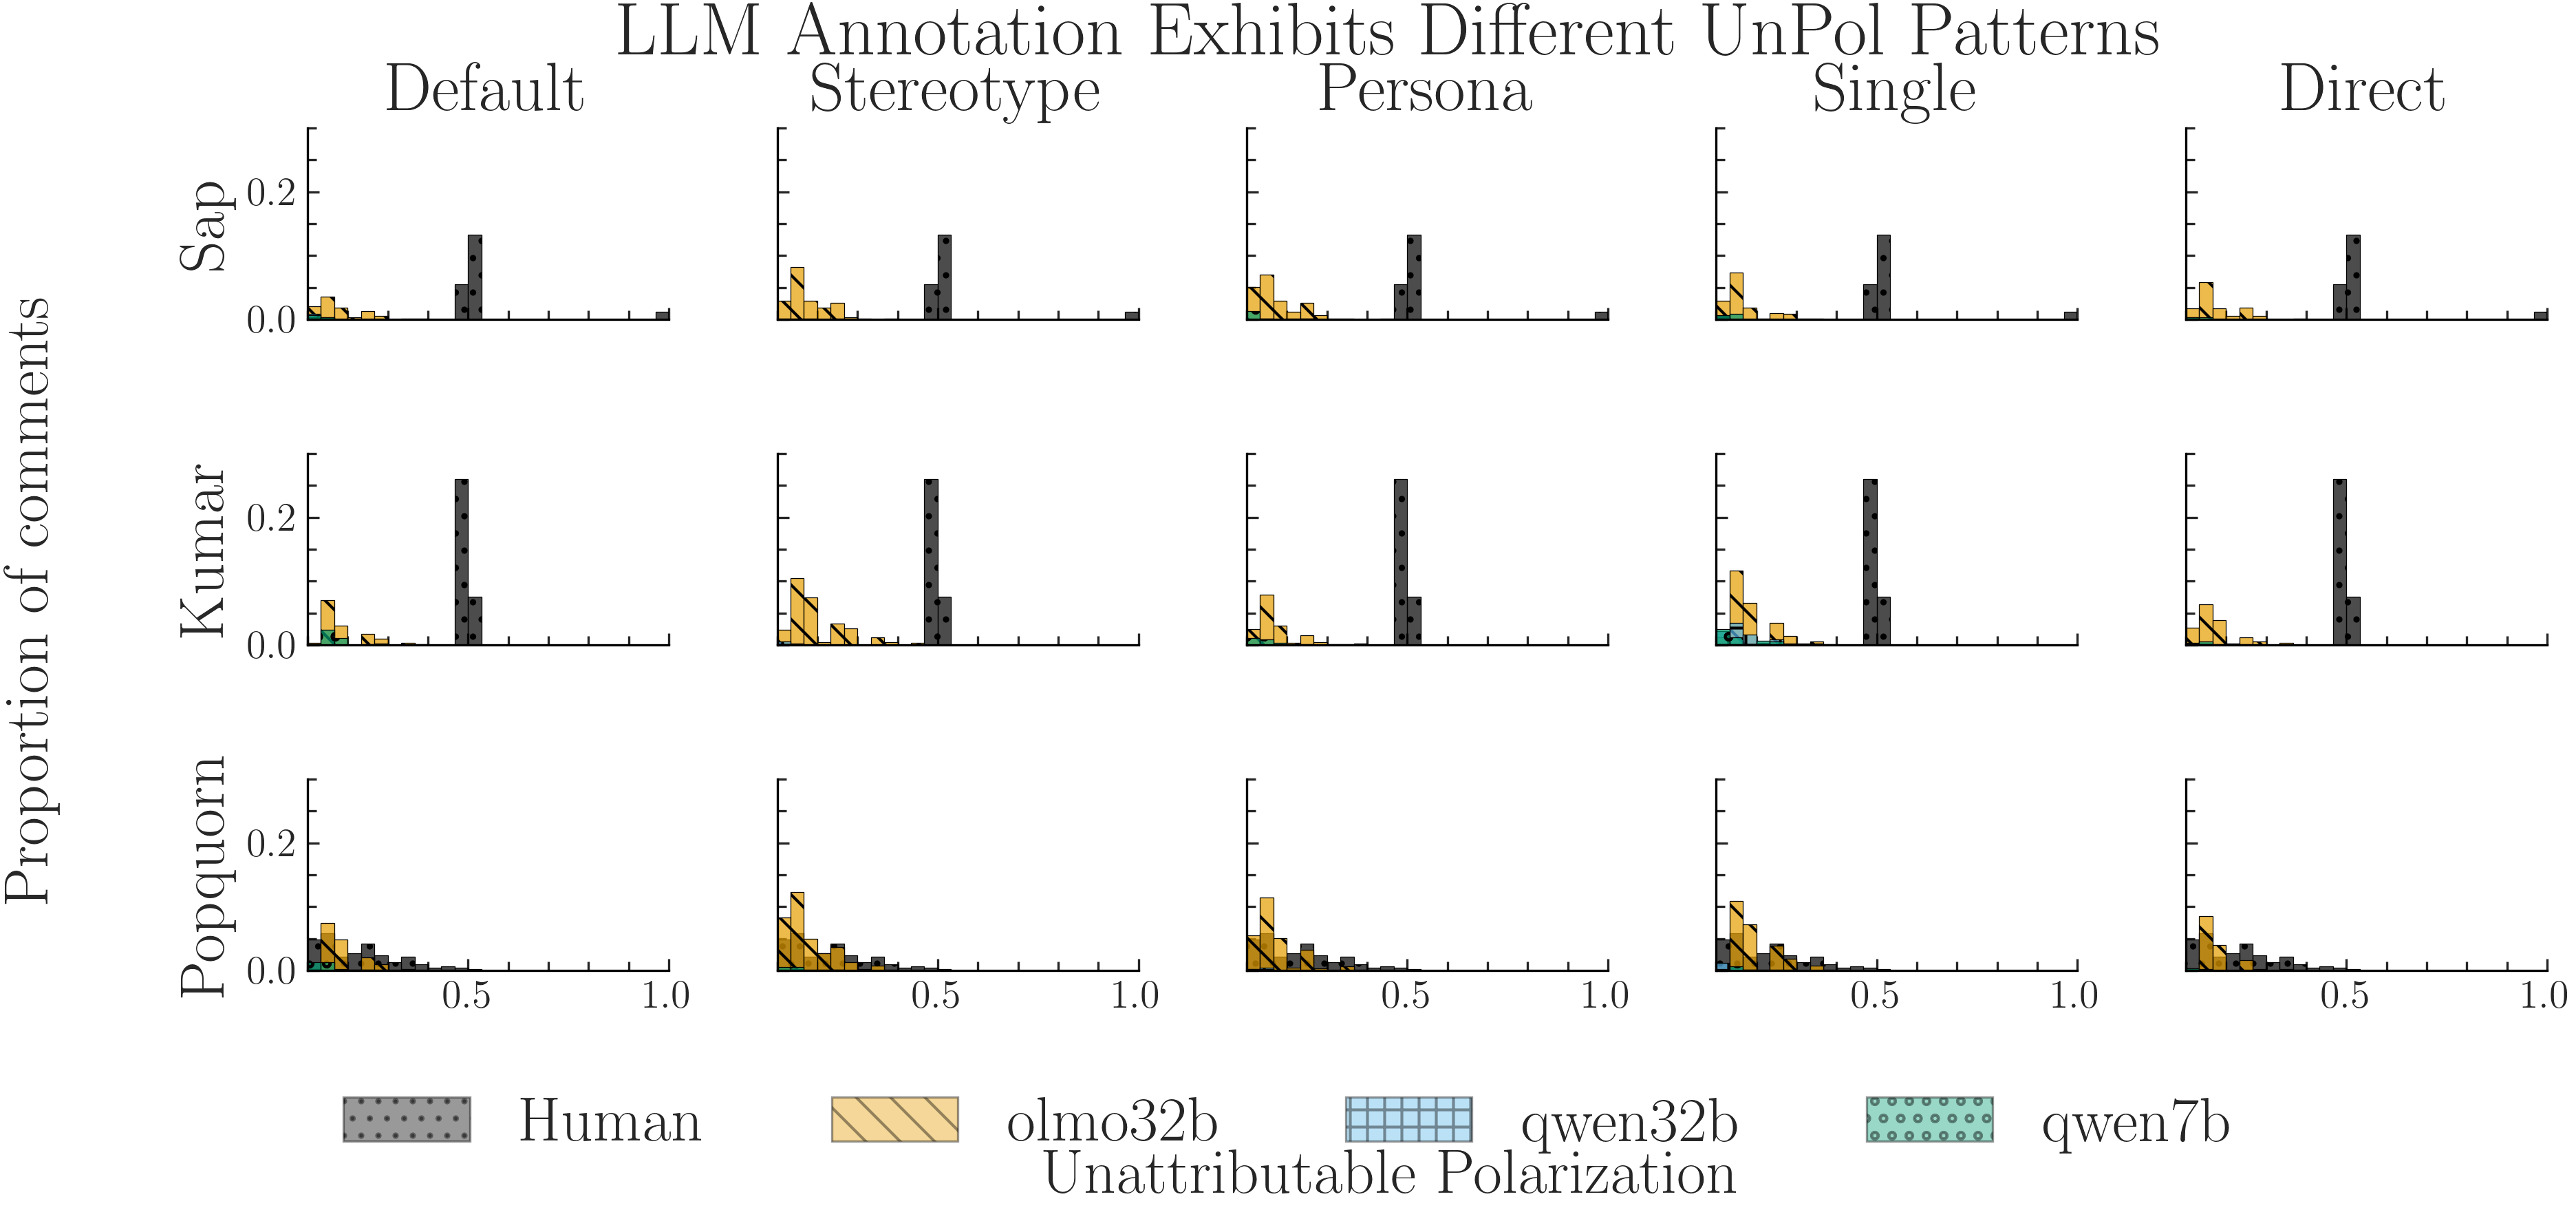
\includegraphics[width=\linewidth]{inherent-polarization-subsampled-n6-histogram.png}
	\caption{Normalized histograms showing the \ac{unpol} exhibited by each model when truncating annotation to six annotations, compared to human annotations for each dataset. Some LLMs fail to show any \ac{unpol}, while the rest show far less than humans. Note that the graph does not include zero \ac{unpol}, and the y-axis is truncated to $[0, 0.3]$.}
	\label{fig:inherent-llms}
\end{figure}

\paragraph{Do LLMs Exhibit UnPol?} We observe \ac{unpol} from most models when repeatedly subsampling six annotators (Fig.~\ref{fig:inherent-llms}). In the case of the Sap and Kumar datasets, human annotators show significantly higher \ac{unpol} values, which is not the case for POPQUORN. Instruction prompts can influence the extent of \ac{unpol}, but inconsistently. Providing adversarial instruction prompts seems to increase \ac{unpol}, although the effect of each prompt seems to be dataset-dependent.

\paragraph{Apunim Analysis} Tables~\ref{tab:llm-apunim-by-prompt-kumar},\ref{tab:llm-apunim-by-prompt-sap},\ref{tab:llm-apunim-by-prompt-popquorn} show the apunim results for the LLM annotation task on the Kumar, Sap and POPQUORN datasets respectively. Apunim values are largely model-dependent, but no other concrete pattern can be discerned. 

\begingroup
\scriptsize
\begin{longtable}[t]{llllllll}
\caption{Aposteriori unimodality results for the LLM annotations of the Kumar et al. 2021 dataset, across instruction prompts. $^{*}p<0.05$, $^{**}p<0.01$, $^{***}p<0.001$.} \label{tab:llm-apunim-by-prompt-kumar} \\
\toprule
 &  &  & Default & Stereotype & Persona & Single & Direct \\
\ac{pc} & Value & Model &  &  &  &  &  \\
\midrule
\endfirsthead
\caption[]{Aposteriori unimodality results for the LLM annotations of the Kumar et al. 2021 dataset, across instruction prompts. $^{*}p<0.05$, $^{**}p<0.01$, $^{***}p<0.001$.} \\
\toprule
 &  &  & Default & Stereotype & Persona & Single & Direct \\
\ac{pc} & Value & Model &  &  &  &  &  \\
\midrule
\endhead
\midrule
\multicolumn{8}{r}{Continued on next page} \\
\midrule
\endfoot
\bottomrule
\endlastfoot
\multirow[t]{24}{*}{Age} & \multirow[t]{3}{*}{1) 18 - 24} & olmo32b & 0.068$^{***}$ & 0.008 & 0.013 & 0.009 & 0.007 \\
 &  & qwen32b & -0.023 & -0.053$^{***}$ & -0.012 & 0.042$^{*}$ & -0.010 \\
 &  & qwen7b & -0.012 & -0.009 & 0.001 & 0.042$^{**}$ & -0.029$^{*}$ \\
\cline{2-8}
 & \multirow[t]{3}{*}{2) 25 - 34} & olmo32b & 0.010 & -0.003 & 0.023 & 0.009 & -0.044$^{**}$ \\
 &  & qwen32b & -0.035$^{*}$ & -0.047$^{**}$ & -0.006 & -0.021 & -0.056$^{***}$ \\
 &  & qwen7b & -0.036$^{**}$ & -0.024$^{*}$ & -0.030 & -0.058$^{***}$ & -0.049$^{***}$ \\
\cline{2-8}
 & \multirow[t]{3}{*}{3) 35 - 44} & olmo32b & -0.029$^{*}$ & 0.011 & -0.001 & -0.018 & -0.027 \\
 &  & qwen32b & -0.042$^{**}$ & 0.029$^{*}$ & 0.003 & -0.017 & -0.018 \\
 &  & qwen7b & -0.051$^{***}$ & -0.069$^{***}$ & -0.079$^{***}$ & -0.028$^{*}$ & -0.074$^{***}$ \\
\cline{2-8}
 & \multirow[t]{3}{*}{4) 45 - 54} & olmo32b & -0.002 & 0.002 & -0.013 & 0.015 & -0.013 \\
 &  & qwen32b & -0.044$^{**}$ & -0.027$^{*}$ & 0.000 & -0.009 & -0.011 \\
 &  & qwen7b & -0.084$^{***}$ & 0.111$^{***}$ & 0.070$^{***}$ & 0.019 & 0.000 \\
\cline{2-8}
 & \multirow[t]{3}{*}{5) 55 - 64} & olmo32b & 0.026 & 0.039$^{**}$ & -0.021 & -0.041$^{**}$ & 0.014 \\
 &  & qwen32b & -0.089$^{***}$ & -0.007 & -0.001 & -0.043$^{*}$ & -0.043$^{**}$ \\
 &  & qwen7b & -0.014 & 0.002 & -0.008 & -0.013 & -0.005 \\
\cline{2-8}
 & \multirow[t]{3}{*}{6) 65 or older} & olmo32b & 0.035$^{**}$ & -0.009 & -0.012 & 0.047$^{**}$ & -0.009 \\
 &  & qwen32b & -0.053$^{**}$ & 0.011 & -0.014 & -0.025 & 0.033$^{*}$ \\
 &  & qwen7b & -0.049$^{***}$ & 0.025$^{*}$ & 0.020 & -0.026 & 0.021 \\
\cline{2-8}
 & \multirow[t]{3}{*}{Prefer not to say} & olmo32b & 0.043$^{**}$ & -0.073$^{***}$ & -0.063$^{***}$ & -0.016 & -0.011 \\
 &  & qwen32b & -0.032$^{*}$ & -0.024 & -0.032 & -0.009 & 0.027$^{*}$ \\
 &  & qwen7b & -0.010 & -0.021 & -0.003 & -0.008 & 0.008 \\
\cline{2-8}
 & \multirow[t]{3}{*}{Under 18} & olmo32b & -0.040$^{**}$ & 0.024 & 0.037$^{**}$ & 0.004 & 0.041$^{**}$ \\
 &  & qwen32b & -0.036$^{*}$ & -0.035$^{*}$ & -0.033 & 0.040$^{*}$ & 0.013 \\
 &  & qwen7b & -0.014 & -0.056$^{***}$ & -0.043$^{*}$ & -0.044$^{**}$ & -0.011 \\
\cline{1-8} \cline{2-8}
\multirow[t]{30}{*}{Education} & \multirow[t]{3}{*}{1) No high school} & olmo32b & 0.007 & 0.013 & 0.007 & -0.011 & -0.011 \\
 &  & qwen32b & 0.009 & 0.024 & 0.000 & 0.043 & 0.019 \\
 &  & qwen7b & -0.028 & -0.092$^{***}$ & -0.052 & -0.012 & -0.013 \\
\cline{2-8}
 & \multirow[t]{3}{*}{2) High School graduate} & olmo32b & 0.100$^{***}$ & -0.003 & -0.020 & 0.107$^{***}$ & -0.084$^{***}$ \\
 &  & qwen32b & 0.016 & -0.027 & 0.008 & 0.023 & -0.054$^{**}$ \\
 &  & qwen7b & -0.028 & -0.059$^{***}$ & -0.015 & -0.026 & -0.047$^{**}$ \\
\cline{2-8}
 & \multirow[t]{3}{*}{3) College, no degree} & olmo32b & -0.070$^{***}$ & 0.041 & -0.069$^{***}$ & 0.001 & 0.015 \\
 &  & qwen32b & -0.017 & 0.031 & 0.010 & -0.031 & 0.003 \\
 &  & qwen7b & -0.022 & 0.013 & -0.022 & -0.020 & -0.024 \\
\cline{2-8}
 & \multirow[t]{3}{*}{4) Associate degree} & olmo32b & -0.023 & 0.033 & -0.012 & 0.019 & 0.045$^{*}$ \\
 &  & qwen32b & -0.030 & -0.011 & -0.031 & -0.022 & -0.015 \\
 &  & qwen7b & 0.016 & 0.048$^{***}$ & -0.017 & -0.010 & -0.018 \\
\cline{2-8}
 & \multirow[t]{3}{*}{5) Bachelor's degree} & olmo32b & 0.034 & 0.026 & 0.008 & -0.007 & 0.052$^{**}$ \\
 &  & qwen32b & -0.011 & -0.014 & 0.010 & -0.034 & 0.046$^{**}$ \\
 &  & qwen7b & 0.022 & 0.027 & 0.028 & -0.016 & -0.055$^{**}$ \\
\cline{2-8}
 & \multirow[t]{3}{*}{6) Master's degree} & olmo32b & -0.006 & 0.006 & 0.029 & -0.010 & 0.005 \\
 &  & qwen32b & 0.014 & -0.024 & -0.042 & 0.013 & -0.006 \\
 &  & qwen7b & -0.030 & 0.015 & 0.009 & 0.022 & 0.044$^{**}$ \\
\cline{2-8}
 & \multirow[t]{3}{*}{7) Professional degree} & olmo32b & -0.007 & 0.009 & -0.031 & -0.012 & -0.016 \\
 &  & qwen32b & 0.004 & -0.045$^{*}$ & -0.020 & -0.000 & -0.028 \\
 &  & qwen7b & 0.014 & 0.012 & 0.003 & -0.027 & 0.007 \\
\cline{2-8}
 & \multirow[t]{3}{*}{8) Doctoral degree} & olmo32b & 0.032 & -0.005 & -0.027 & 0.027 & 0.018 \\
 &  & qwen32b & -0.013 & -0.022 & 0.019 & -0.018 & -0.035$^{*}$ \\
 &  & qwen7b & 0.005 & 0.060$^{***}$ & 0.011 & -0.012 & 0.010 \\
\cline{2-8}
 & \multirow[t]{3}{*}{Other} & olmo32b & 0.025 & -0.038 & -0.014 & -0.008 & -0.021 \\
 &  & qwen32b & -0.031 & 0.040$^{*}$ & -0.001 & -0.017 & 0.040$^{*}$ \\
 &  & qwen7b & 0.015 & -0.010 & -0.011 & -0.036 & 0.045$^{**}$ \\
\cline{2-8}
 & \multirow[t]{3}{*}{Prefer not to say} & olmo32b & 0.008 & -0.045 & -0.011 & 0.025 & 0.020 \\
 &  & qwen32b & 0.050$^{*}$ & 0.003 & 0.024 & -0.006 & 0.018 \\
 &  & qwen7b & 0.006 & -0.045$^{**}$ & -0.020 & 0.034 & -0.014 \\
\cline{1-8} \cline{2-8}
\multirow[t]{21}{*}{Ethnicity} & \multirow[t]{3}{*}{Asian} & olmo32b & -0.015 & -0.015 & 0.001 & -0.006 & 0.001 \\
 &  & qwen32b & -0.010 & -0.017 & 0.016 & 0.028 & -0.006 \\
 &  & qwen7b & 0.028$^{*}$ & 0.002 & -0.015 & 0.007 & -0.030$^{*}$ \\
\cline{2-8}
 & \multirow[t]{3}{*}{Black} & olmo32b & 0.017 & -0.032$^{*}$ & -0.062$^{***}$ & -0.001 & -0.073$^{***}$ \\
 &  & qwen32b & 0.018 & -0.027 & 0.027 & -0.027 & 0.009 \\
 &  & qwen7b & 0.024 & 0.016 & 0.024 & -0.035$^{*}$ & 0.043$^{***}$ \\
\cline{2-8}
 & \multirow[t]{3}{*}{Hispanic} & olmo32b & 0.055$^{***}$ & -0.005 & -0.006 & 0.024 & 0.033$^{**}$ \\
 &  & qwen32b & -0.033$^{*}$ & 0.007 & -0.008 & -0.019 & -0.036$^{**}$ \\
 &  & qwen7b & -0.021 & -0.017 & 0.024 & 0.005 & 0.028$^{*}$ \\
\cline{2-8}
 & \multirow[t]{3}{*}{Multiracial} & olmo32b & -0.014 & -0.011 & -0.011 & -0.023 & 0.009 \\
 &  & qwen32b & -0.052$^{**}$ & -0.021 & -0.044$^{**}$ & -0.008 & -0.025$^{*}$ \\
 &  & qwen7b & -0.022 & -0.038$^{***}$ & -0.002 & -0.021 & 0.004 \\
\cline{2-8}
 & \multirow[t]{3}{*}{Other} & olmo32b & 0.014 & 0.059$^{***}$ & 0.022 & 0.032$^{*}$ & 0.033$^{**}$ \\
 &  & qwen32b & -0.007 & -0.010 & -0.018 & 0.023 & -0.040$^{**}$ \\
 &  & qwen7b & -0.026 & 0.019 & -0.002 & 0.003 & -0.013 \\
\cline{2-8}
 & \multirow[t]{3}{*}{Unknown} & olmo32b & -0.022 & -0.013 & -0.007 & -0.001 & 0.015 \\
 &  & qwen32b & -0.017 & -0.029 & -0.002 & 0.013 & 0.068$^{***}$ \\
 &  & qwen7b & 0.021 & -0.002 & -0.030 & -0.007 & -0.006 \\
\cline{2-8}
 & \multirow[t]{3}{*}{White} & olmo32b & -0.024 & 0.024 & 0.004 & -0.033$^{*}$ & 0.005 \\
 &  & qwen32b & 0.022 & 0.017 & -0.024 & 0.022 & -0.026$^{*}$ \\
 &  & qwen7b & -0.039$^{**}$ & 0.014 & -0.011 & 0.020 & -0.012 \\
\cline{1-8} \cline{2-8}
\multirow[t]{12}{*}{Gender} & \multirow[t]{3}{*}{Female} & olmo32b & 0.014 & 0.001 & 0.029$^{***}$ & -0.004 & -0.024$^{*}$ \\
 &  & qwen32b & 0.031$^{*}$ & 0.016 & 0.007 & -0.006 & 0.017 \\
 &  & qwen7b & 0.012 & -0.033$^{***}$ & -0.006 & -0.008 & -0.015 \\
\cline{2-8}
 & \multirow[t]{3}{*}{Male} & olmo32b & 0.041$^{***}$ & 0.002 & 0.012 & 0.001 & 0.053$^{***}$ \\
 &  & qwen32b & -0.023 & -0.005 & -0.019 & -0.001 & 0.016 \\
 &  & qwen7b & -0.032$^{**}$ & 0.013 & -0.003 & 0.022 & 0.028$^{*}$ \\
\cline{2-8}
 & \multirow[t]{3}{*}{Nonbinary} & olmo32b & 0.003 & 0.007 & 0.013 & -0.011 & -0.032$^{**}$ \\
 &  & qwen32b & -0.027 & -0.024 & -0.007 & -0.053$^{***}$ & -0.063$^{***}$ \\
 &  & qwen7b & -0.001 & 0.013 & -0.013 & 0.002 & 0.020 \\
\cline{2-8}
 & \multirow[t]{3}{*}{Unknown} & olmo32b & -0.015 & -0.002 & -0.010 & -0.034$^{***}$ & -0.017 \\
 &  & qwen32b & -0.021 & -0.013 & 0.005 & 0.020 & 0.001 \\
 &  & qwen7b & -0.014 & -0.020$^{*}$ & 0.012 & 0.002 & -0.019 \\
\cline{1-8} \cline{2-8}
\multirow[t]{6}{*}{Has Been Targeted} & \multirow[t]{3}{*}{False} & olmo32b & -0.002 & 0.011 & -0.006 & 0.016 & -0.019 \\
 &  & qwen32b & 0.019 & -0.018 & -0.010 & 0.001 & 0.002 \\
 &  & qwen7b & -0.083$^{***}$ & 0.019 & 0.011 & 0.016 & -0.031$^{**}$ \\
\cline{2-8}
 & \multirow[t]{3}{*}{True} & olmo32b & 0.021 & 0.008 & -0.001 & -0.023 & 0.022 \\
 &  & qwen32b & -0.021 & -0.010 & -0.004 & 0.002 & -0.012 \\
 &  & qwen7b & 0.049$^{***}$ & -0.018 & -0.013 & -0.027 & 0.038$^{**}$ \\
\cline{1-8} \cline{2-8}
\multirow[t]{9}{*}{Is Parent} & \multirow[t]{3}{*}{No} & olmo32b & -0.018 & 0.016 & 0.000 & -0.003 & -0.008 \\
 &  & qwen32b & -0.036$^{*}$ & -0.025 & -0.023 & 0.008 & -0.024 \\
 &  & qwen7b & -0.001 & 0.010 & -0.013 & 0.008 & -0.016 \\
\cline{2-8}
 & \multirow[t]{3}{*}{Prefer not to say} & olmo32b & -0.020 & 0.009 & 0.015 & 0.004 & -0.015 \\
 &  & qwen32b & 0.025 & 0.014 & 0.024 & 0.015 & 0.014 \\
 &  & qwen7b & -0.002 & -0.013 & 0.018 & -0.022 & -0.009 \\
\cline{2-8}
 & \multirow[t]{3}{*}{Yes} & olmo32b & 0.010 & 0.006 & 0.007 & 0.018 & 0.006 \\
 &  & qwen32b & -0.003 & -0.000 & 0.005 & 0.009 & 0.012 \\
 &  & qwen7b & -0.021 & 0.003 & -0.015 & 0.009 & 0.001 \\
\cline{1-8} \cline{2-8}
\multirow[t]{9}{*}{Is Transgender} & \multirow[t]{3}{*}{No} & olmo32b & -0.020 & 0.015 & -0.008 & 0.021 & -0.004 \\
 &  & qwen32b & 0.005 & 0.021 & -0.004 & -0.003 & -0.013 \\
 &  & qwen7b & -0.004 & -0.024$^{**}$ & -0.005 & -0.010 & -0.001 \\
\cline{2-8}
 & \multirow[t]{3}{*}{Prefer not to say} & olmo32b & 0.023 & -0.027$^{**}$ & 0.013 & -0.013 & -0.020 \\
 &  & qwen32b & -0.001 & -0.005 & 0.012 & 0.011 & -0.003 \\
 &  & qwen7b & 0.041$^{***}$ & -0.024$^{**}$ & 0.008 & -0.008 & -0.016 \\
\cline{2-8}
 & \multirow[t]{3}{*}{Yes} & olmo32b & 0.004 & -0.028$^{**}$ & -0.015 & 0.007 & -0.005 \\
 &  & qwen32b & -0.026 & -0.023 & -0.003 & 0.013 & 0.005 \\
 &  & qwen7b & -0.039$^{***}$ & 0.033$^{***}$ & -0.015 & 0.016 & -0.005 \\
\cline{1-8} \cline{2-8}
\multirow[t]{15}{*}{Political Affiliation} & \multirow[t]{3}{*}{Conservative} & olmo32b & 0.001 & 0.076$^{***}$ & 0.018 & -0.005 & -0.010 \\
 &  & qwen32b & -0.025 & 0.031$^{*}$ & -0.012 & 0.008 & 0.007 \\
 &  & qwen7b & -0.039$^{***}$ & 0.044$^{***}$ & -0.001 & 0.010 & -0.008 \\
\cline{2-8}
 & \multirow[t]{3}{*}{Independent} & olmo32b & -0.012 & -0.034$^{**}$ & -0.017 & 0.026$^{*}$ & -0.007 \\
 &  & qwen32b & 0.003 & -0.005 & -0.008 & -0.004 & -0.013 \\
 &  & qwen7b & 0.020 & -0.011 & -0.000 & 0.023$^{*}$ & 0.011 \\
\cline{2-8}
 & \multirow[t]{3}{*}{Liberal} & olmo32b & -0.005 & -0.028$^{**}$ & 0.013 & -0.003 & -0.002 \\
 &  & qwen32b & 0.013 & 0.013 & -0.003 & -0.018 & -0.011 \\
 &  & qwen7b & -0.024$^{*}$ & 0.030$^{**}$ & -0.009 & -0.037$^{***}$ & -0.025$^{*}$ \\
\cline{2-8}
 & \multirow[t]{3}{*}{Other} & olmo32b & 0.006 & -0.063$^{***}$ & -0.000 & 0.004 & 0.005 \\
 &  & qwen32b & 0.018 & -0.029$^{*}$ & 0.008 & 0.017 & -0.010 \\
 &  & qwen7b & 0.006 & -0.014 & -0.010 & -0.004 & -0.013 \\
\cline{2-8}
 & \multirow[t]{3}{*}{Prefer not to say} & olmo32b & -0.003 & -0.003 & 0.004 & -0.001 & -0.010 \\
 &  & qwen32b & 0.009 & -0.009 & -0.012 & -0.015 & -0.009 \\
 &  & qwen7b & 0.045$^{***}$ & -0.006 & 0.007 & -0.053$^{***}$ & 0.003 \\
\cline{1-8} \cline{2-8}
\multirow[t]{15}{*}{Religion Important} & \multirow[t]{3}{*}{1) No} & olmo32b & -0.003 & 0.032$^{**}$ & 0.018 & -0.029$^{*}$ & -0.011 \\
 &  & qwen32b & 0.016 & 0.004 & -0.009 & -0.003 & -0.013 \\
 &  & qwen7b & 0.006 & -0.043$^{***}$ & -0.044$^{***}$ & -0.036$^{***}$ & 0.005 \\
\cline{2-8}
 & \multirow[t]{3}{*}{2) Not very} & olmo32b & 0.005 & -0.031$^{**}$ & -0.026$^{**}$ & -0.006 & -0.024$^{*}$ \\
 &  & qwen32b & -0.015 & 0.011 & -0.016 & 0.008 & -0.006 \\
 &  & qwen7b & -0.044$^{***}$ & -0.084$^{***}$ & -0.050$^{***}$ & -0.051$^{***}$ & -0.053$^{***}$ \\
\cline{2-8}
 & \multirow[t]{3}{*}{3) Somewhat} & olmo32b & -0.004 & 0.060$^{***}$ & 0.011 & -0.002 & 0.010 \\
 &  & qwen32b & -0.007 & 0.019 & -0.007 & 0.048$^{***}$ & -0.020 \\
 &  & qwen7b & -0.000 & -0.085$^{***}$ & -0.058$^{***}$ & -0.039$^{***}$ & -0.059$^{***}$ \\
\cline{2-8}
 & \multirow[t]{3}{*}{4) Very} & olmo32b & -0.027$^{*}$ & -0.019 & -0.007 & -0.001 & -0.028$^{*}$ \\
 &  & qwen32b & -0.019 & -0.030$^{*}$ & -0.005 & -0.006 & 0.016 \\
 &  & qwen7b & -0.033$^{**}$ & 0.167$^{***}$ & 0.098$^{***}$ & 0.027$^{*}$ & 0.051$^{***}$ \\
\cline{2-8}
 & \multirow[t]{3}{*}{Prefer not to say} & olmo32b & 0.012 & -0.010 & 0.002 & -0.001 & -0.025$^{*}$ \\
 &  & qwen32b & -0.001 & -0.001 & 0.004 & 0.020 & -0.014 \\
 &  & qwen7b & 0.002 & 0.003 & 0.012 & -0.015 & -0.017 \\
\cline{1-8} \cline{2-8}
\multirow[t]{6}{*}{Seen Toxicity} & \multirow[t]{3}{*}{False} & olmo32b & -0.002 & -0.011 & 0.029$^{*}$ & 0.000 & -0.008 \\
 &  & qwen32b & 0.009 & 0.001 & 0.006 & -0.011 & 0.018 \\
 &  & qwen7b & 0.048$^{***}$ & -0.023$^{*}$ & -0.007 & 0.001 & -0.009 \\
\cline{2-8}
 & \multirow[t]{3}{*}{True} & olmo32b & -0.010 & 0.003 & -0.005 & 0.004 & 0.010 \\
 &  & qwen32b & 0.008 & -0.005 & -0.017 & 0.024 & -0.010 \\
 &  & qwen7b & -0.062$^{***}$ & 0.020$^{*}$ & -0.005 & -0.012 & 0.007 \\
\cline{1-8} \cline{2-8}
\multirow[t]{15}{*}{Sexual Orientation} & \multirow[t]{3}{*}{Bisexual} & olmo32b & -0.001 & -0.003 & -0.018 & -0.020$^{*}$ & -0.001 \\
 &  & qwen32b & -0.012 & -0.005 & 0.011 & -0.012 & 0.028$^{*}$ \\
 &  & qwen7b & -0.011 & 0.004 & 0.008 & 0.010 & 0.003 \\
\cline{2-8}
 & \multirow[t]{3}{*}{Heterosexual} & olmo32b & 0.019 & 0.019 & 0.008 & 0.016 & -0.011 \\
 &  & qwen32b & -0.008 & -0.004 & 0.022 & 0.012 & -0.035$^{**}$ \\
 &  & qwen7b & 0.005 & -0.037$^{***}$ & 0.014 & -0.007 & 0.014 \\
\cline{2-8}
 & \multirow[t]{3}{*}{Homosexual} & olmo32b & 0.024 & -0.014 & -0.016 & 0.024$^{*}$ & 0.012 \\
 &  & qwen32b & -0.005 & 0.004 & -0.007 & 0.042$^{**}$ & 0.003 \\
 &  & qwen7b & -0.010 & 0.043$^{***}$ & 0.041$^{**}$ & 0.038$^{**}$ & -0.006 \\
\cline{2-8}
 & \multirow[t]{3}{*}{Other} & olmo32b & 0.006 & -0.024 & 0.013 & -0.032$^{**}$ & -0.022 \\
 &  & qwen32b & -0.003 & -0.000 & 0.009 & 0.008 & -0.011 \\
 &  & qwen7b & -0.036$^{**}$ & 0.004 & -0.033$^{*}$ & -0.018 & 0.041$^{***}$ \\
\cline{2-8}
 & \multirow[t]{3}{*}{Prefer not to say} & olmo32b & -0.007 & 0.011 & 0.007 & 0.019$^{*}$ & -0.003 \\
 &  & qwen32b & -0.012 & 0.014 & -0.009 & -0.021 & -0.009 \\
 &  & qwen7b & 0.000 & -0.042$^{***}$ & -0.025 & -0.007 & -0.034$^{**}$ \\
\cline{1-8} \cline{2-8}
\multirow[t]{15}{*}{Technology Impact} & \multirow[t]{3}{*}{1) Very negative} & olmo32b & -0.009 & 0.016 & 0.003 & -0.018 & 0.013 \\
 &  & qwen32b & 0.007 & 0.001 & 0.018 & 0.030$^{*}$ & 0.056$^{***}$ \\
 &  & qwen7b & -0.005 & -0.028$^{**}$ & -0.051$^{***}$ & -0.052$^{***}$ & 0.004 \\
\cline{2-8}
 & \multirow[t]{3}{*}{2) Somewhat negative} & olmo32b & -0.001 & 0.017 & 0.037$^{***}$ & -0.006 & 0.016 \\
 &  & qwen32b & 0.008 & -0.013 & 0.002 & 0.013 & -0.006 \\
 &  & qwen7b & 0.035$^{**}$ & -0.026$^{**}$ & -0.018 & -0.035$^{**}$ & 0.032$^{**}$ \\
\cline{2-8}
 & \multirow[t]{3}{*}{3) Neutral} & olmo32b & -0.017 & 0.003 & -0.016 & 0.018 & -0.009 \\
 &  & qwen32b & 0.007 & -0.008 & -0.016 & -0.004 & -0.030$^{**}$ \\
 &  & qwen7b & 0.005 & -0.031$^{***}$ & -0.016 & 0.004 & -0.004 \\
\cline{2-8}
 & \multirow[t]{3}{*}{4) Somewhat positive} & olmo32b & 0.006 & -0.004 & -0.012 & -0.003 & 0.013 \\
 &  & qwen32b & -0.039$^{**}$ & -0.026 & 0.001 & -0.051$^{***}$ & -0.004 \\
 &  & qwen7b & -0.023 & 0.065$^{***}$ & 0.046$^{***}$ & 0.003 & 0.022$^{*}$ \\
\cline{2-8}
 & \multirow[t]{3}{*}{5) Very positive} & olmo32b & 0.013 & 0.043$^{***}$ & -0.025$^{**}$ & 0.004 & -0.025 \\
 &  & qwen32b & -0.028 & 0.013 & -0.023 & 0.005 & -0.036$^{**}$ \\
 &  & qwen7b & 0.001 & 0.026$^{**}$ & 0.008 & -0.012 & -0.050$^{***}$ \\
\cline{1-8} \cline{2-8}
\multirow[t]{15}{*}{Toxicity Problem} & \multirow[t]{3}{*}{1) Never} & olmo32b & 0.003 & 0.004 & 0.032$^{***}$ & 0.029$^{**}$ & -0.012 \\
 &  & qwen32b & -0.050$^{***}$ & -0.029$^{**}$ & -0.074$^{***}$ & -0.322$^{***}$ & -0.130$^{***}$ \\
 &  & qwen7b & -0.054$^{***}$ & -0.049$^{***}$ & -0.043$^{***}$ & -0.065$^{***}$ & -0.084$^{***}$ \\
\cline{2-8}
 & \multirow[t]{3}{*}{2) Rarely} & olmo32b & -0.038$^{***}$ & -0.006 & 0.023$^{**}$ & -0.009 & -0.059$^{***}$ \\
 &  & qwen32b & -0.071$^{***}$ & -0.042$^{***}$ & -0.108$^{***}$ & -0.343$^{***}$ & -0.173$^{***}$ \\
 &  & qwen7b & 0.002 & -0.091$^{***}$ & -0.066$^{***}$ & -0.016 & -0.091$^{***}$ \\
\cline{2-8}
 & \multirow[t]{3}{*}{3) Occasionally} & olmo32b & -0.066$^{***}$ & -0.008 & -0.023$^{**}$ & -0.059$^{***}$ & -0.046$^{***}$ \\
 &  & qwen32b & -0.061$^{***}$ & -0.056$^{***}$ & -0.063$^{***}$ & -0.278$^{***}$ & -0.142$^{***}$ \\
 &  & qwen7b & -0.143$^{***}$ & -0.137$^{***}$ & -0.078$^{***}$ & -0.021$^{*}$ & -0.178$^{***}$ \\
\cline{2-8}
 & \multirow[t]{3}{*}{4) Frequently} & olmo32b & 0.018 & -0.020 & -0.021$^{*}$ & -0.006 & 0.003 \\
 &  & qwen32b & -0.047$^{***}$ & -0.050$^{***}$ & -0.077$^{***}$ & -0.269$^{***}$ & -0.147$^{***}$ \\
 &  & qwen7b & 0.004 & 0.168$^{***}$ & 0.088$^{***}$ & -0.176$^{***}$ & 0.064$^{***}$ \\
\cline{2-8}
 & \multirow[t]{3}{*}{5) Very Frequently} & olmo32b & 0.036$^{***}$ & -0.044$^{***}$ & -0.043$^{***}$ & -0.011 & -0.003 \\
 &  & qwen32b & -0.055$^{***}$ & -0.062$^{***}$ & -0.087$^{***}$ & -0.254$^{***}$ & -0.123$^{***}$ \\
 &  & qwen7b & -0.214$^{***}$ & 0.061$^{***}$ & 0.062$^{***}$ & 0.085$^{***}$ & -0.012 \\
\cline{1-8} \cline{2-8}
\end{longtable}

\begin{longtable}[t]{llllllll}
\caption{Aposteriori unimodality results for the LLM annotations of the Sap et al. 2022 dataset, across instruction prompts. $^{*}p<0.05$, $^{**}p<0.01$, $^{***}p<0.001$.} \label{tab:llm-apunim-by-prompt-sap} \\
\toprule
 &  &  & Default & Stereotype & Persona & Single & Direct \\
\ac{sdd} & Value & Model &  &  &  &  &  \\
\midrule
\endfirsthead
\caption[]{Aposteriori unimodality results for the LLM annotations of the Sap et al. 2022 dataset, across instruction prompts. $^{*}p<0.05$, $^{**}p<0.01$, $^{***}p<0.001$.} \\
\toprule
 &  &  & Default & Stereotype & Persona & Single & Direct \\
\ac{sdd} & Value & Model &  &  &  &  &  \\
\midrule
\endhead
\midrule
\multicolumn{8}{r}{Continued on next page} \\
\midrule
\endfoot
\bottomrule
\endlastfoot
\multirow[t]{27}{*}{Age} & \multirow[t]{9}{*}{1) Gen. X+} & llama8b & -0.009 & -0.018 & -0.023 & 0.017 & -0.030$^{**}$ \\
 &  & olmo32b & -0.006 & -0.010 & 0.012 & -0.031 & -0.021 \\
 &  & olmo7b & 0.023$^{*}$ & -0.001 & 0.009 & 0.047$^{***}$ & 0.017$^{*}$ \\
 &  & qwen32b & 0.208$^{***}$ & 0.061$^{***}$ & 0.120$^{***}$ & 0.189$^{***}$ & 0.184$^{***}$ \\
 &  & qwen7b & 0.152$^{***}$ & 0.090$^{***}$ & 0.147$^{***}$ & 0.055$^{***}$ & 0.181$^{***}$ \\
 &  & mistral7b & 0.059$^{**}$ & 0.004 & 0.054$^{**}$ & -0.018 & -0.000 \\
 &  & mistral24b & 0.131$^{***}$ & 0.006 & 0.079$^{**}$ & -0.025 & 0.051$^{***}$ \\
 &  & gemma7b & 0.021 & 0.004 & 0.047$^{**}$ & 0.038$^{*}$ & -0.014 \\
 &  & gemma31b & -0.024 & 0.009 & -0.098$^{***}$ & 0.004 & -0.043 \\
\cline{2-8}
 & \multirow[t]{9}{*}{2) Millennial} & llama8b & -0.019 & 0.011 & 0.016 & 0.140$^{***}$ & -0.013 \\
 &  & olmo32b & -0.009 & -0.042$^{*}$ & -0.037$^{*}$ & -0.014 & -0.023 \\
 &  & olmo7b & 0.031$^{**}$ & -0.052$^{***}$ & 0.038$^{***}$ & -0.053$^{***}$ & -0.033$^{***}$ \\
 &  & qwen32b & 0.249$^{***}$ & 0.059$^{***}$ & 0.190$^{***}$ & 0.137$^{***}$ & 0.214$^{***}$ \\
 &  & qwen7b & 0.246$^{***}$ & 0.139$^{***}$ & 0.219$^{***}$ & 0.098$^{***}$ & 0.182$^{***}$ \\
 &  & mistral7b & 0.017 & 0.008 & -0.043$^{*}$ & -0.058$^{**}$ & -0.011 \\
 &  & mistral24b & 0.177$^{***}$ & 0.036$^{**}$ & 0.088$^{***}$ & 0.166$^{***}$ & 0.081$^{***}$ \\
 &  & gemma7b & 0.021 & -0.014 & -0.020 & -0.009 & 0.025 \\
 &  & gemma31b & 0.085$^{*}$ & 0.074$^{**}$ & 0.061$^{*}$ & 0.042 & 0.097$^{***}$ \\
\cline{2-8}
 & \multirow[t]{9}{*}{3) Gen. Z} & llama8b & 0.072$^{***}$ & 0.107$^{***}$ & 0.021 & 0.079$^{*}$ & 0.079$^{***}$ \\
 &  & olmo32b & 0.054$^{**}$ & 0.023 & 0.039$^{*}$ & 0.022 & 0.054$^{**}$ \\
 &  & olmo7b & -0.020$^{*}$ & 0.018 & 0.017 & 0.004 & -0.015$^{*}$ \\
 &  & qwen32b & 0.124$^{***}$ & 0.122$^{***}$ & 0.204$^{***}$ & 0.083$^{***}$ & 0.140$^{***}$ \\
 &  & qwen7b & 0.007 & 0.109$^{***}$ & -0.014 & 0.137$^{***}$ & 0.133$^{***}$ \\
 &  & mistral7b & 0.094$^{***}$ & 0.047$^{*}$ & 0.014 & 0.022 & 0.011 \\
 &  & mistral24b & -0.062$^{***}$ & 0.162$^{***}$ & 0.000 & -0.022 & 0.050$^{***}$ \\
 &  & gemma7b & -0.014 & 0.003 & 0.002 & 0.011 & 0.019 \\
 &  & gemma31b & 0.124$^{**}$ & 0.188$^{***}$ & 0.202$^{***}$ & 0.105$^{**}$ & 0.135$^{***}$ \\
\cline{1-8} \cline{2-8}
\multirow[t]{45}{*}{Ethnicity} & \multirow[t]{9}{*}{black} & llama8b & -0.005 & 0.076$^{***}$ & -0.077$^{***}$ & -0.070 & 0.013 \\
 &  & olmo32b & 0.017 & 0.041 & 0.079$^{***}$ & 0.020 & 0.013 \\
 &  & olmo7b & 0.017 & 0.007 & 0.004 & -0.005 & 0.029$^{**}$ \\
 &  & qwen32b & 0.010 & 0.202$^{***}$ & 0.110$^{***}$ & 0.043$^{*}$ & 0.080$^{***}$ \\
 &  & qwen7b & 0.047$^{***}$ & 0.126$^{***}$ & 0.049$^{***}$ & 0.050$^{***}$ & -0.021 \\
 &  & mistral7b & 0.054$^{**}$ & 0.302$^{***}$ & 0.214$^{***}$ & 0.099$^{***}$ & 0.162$^{***}$ \\
 &  & mistral24b & 0.095$^{***}$ & 0.430$^{***}$ & 0.032 & -0.049 & 0.174$^{***}$ \\
 &  & gemma7b & 0.023 & 0.069$^{***}$ & 0.032$^{*}$ & 0.044$^{***}$ & 0.099$^{***}$ \\
 &  & gemma31b & 0.148$^{***}$ & 0.285$^{***}$ & 0.375$^{***}$ & 0.138$^{***}$ & 0.295$^{***}$ \\
\cline{2-8}
 & \multirow[t]{9}{*}{hisp} & llama8b & 0.012 & -0.017 & 0.088$^{***}$ & 0.142$^{*}$ & 0.037$^{***}$ \\
 &  & olmo32b & -0.020 & 0.005 & -0.026 & 0.012 & 0.018 \\
 &  & olmo7b & 0.050$^{***}$ & -0.016 & -0.008 & -0.020 & 0.023$^{*}$ \\
 &  & qwen32b & 0.031 & 0.172$^{***}$ & 0.047$^{**}$ & -0.007 & 0.094$^{***}$ \\
 &  & qwen7b & 0.038$^{**}$ & 0.149$^{***}$ & 0.052$^{***}$ & 0.068$^{***}$ & 0.085$^{***}$ \\
 &  & mistral7b & 0.031 & 0.058$^{**}$ & -0.019 & 0.004 & -0.050$^{*}$ \\
 &  & mistral24b & 0.090$^{***}$ & 0.277$^{***}$ & -0.005 & 0.114$^{*}$ & 0.149$^{***}$ \\
 &  & gemma7b & 0.059$^{***}$ & 0.072$^{***}$ & 0.009 & 0.055$^{***}$ & 0.062$^{***}$ \\
 &  & gemma31b & 0.064 & 0.120$^{***}$ & 0.076$^{**}$ & 0.102$^{***}$ & 0.141$^{***}$ \\
\cline{2-8}
 & \multirow[t]{9}{*}{middleEastern} & llama8b & -0.030 & 0.067$^{***}$ & 0.119$^{***}$ & 0.032 & 0.008 \\
 &  & olmo32b & -0.013 & 0.028 & -0.008 & 0.028 & 0.032 \\
 &  & olmo7b & -0.049$^{***}$ & 0.003 & -0.025$^{**}$ & 0.033$^{*}$ & 0.009 \\
 &  & qwen32b & 0.052$^{**}$ & 0.277$^{***}$ & 0.093$^{***}$ & 0.078$^{***}$ & 0.094$^{***}$ \\
 &  & qwen7b & -0.001 & 0.046$^{***}$ & 0.021 & -0.075$^{***}$ & 0.002 \\
 &  & mistral7b & 0.009 & 0.073$^{***}$ & 0.022 & -0.037 & 0.015 \\
 &  & mistral24b & 0.082$^{***}$ & 0.294$^{***}$ & 0.052 & 0.041 & 0.082$^{***}$ \\
 &  & gemma7b & 0.041$^{*}$ & 0.070$^{***}$ & 0.004 & 0.072$^{***}$ & 0.019 \\
 &  & gemma31b & 0.105$^{**}$ & 0.187$^{***}$ & 0.104$^{***}$ & 0.138$^{***}$ & 0.038 \\
\cline{2-8}
 & \multirow[t]{9}{*}{other} & llama8b & -0.015 & -0.045$^{***}$ & -0.003 & 0.082 & -0.067$^{***}$ \\
 &  & olmo32b & -0.014 & 0.024 & -0.006 & -0.024 & 0.022 \\
 &  & olmo7b & -0.031$^{***}$ & -0.025$^{*}$ & 0.043$^{***}$ & -0.038$^{*}$ & 0.069$^{***}$ \\
 &  & qwen32b & 0.031 & 0.165$^{***}$ & 0.087$^{***}$ & 0.094$^{***}$ & 0.084$^{***}$ \\
 &  & qwen7b & 0.072$^{***}$ & 0.106$^{***}$ & 0.038$^{**}$ & 0.116$^{***}$ & 0.038$^{**}$ \\
 &  & mistral7b & 0.118$^{***}$ & 0.092$^{***}$ & 0.036 & 0.018 & 0.074$^{***}$ \\
 &  & mistral24b & 0.002 & 0.123$^{***}$ & 0.033 & 0.045 & 0.111$^{***}$ \\
 &  & gemma7b & -0.013 & 0.117$^{***}$ & 0.045$^{**}$ & -0.001 & 0.033 \\
 &  & gemma31b & 0.111$^{**}$ & 0.085$^{***}$ & 0.021 & 0.094$^{**}$ & 0.025 \\
\cline{2-8}
 & \multirow[t]{9}{*}{white} & llama8b & -0.023 & 0.020 & -0.043$^{*}$ & -0.022 & 0.057$^{***}$ \\
 &  & olmo32b & 0.020 & -0.018 & -0.022 & 0.015 & -0.011 \\
 &  & olmo7b & 0.034$^{***}$ & 0.002 & 0.066$^{***}$ & -0.002 & 0.073$^{***}$ \\
 &  & qwen32b & 0.086$^{***}$ & 0.186$^{***}$ & 0.072$^{***}$ & 0.050$^{**}$ & 0.044$^{**}$ \\
 &  & qwen7b & 0.068$^{***}$ & 0.023$^{*}$ & -0.003 & 0.058$^{***}$ & 0.005 \\
 &  & mistral7b & 0.071$^{***}$ & 0.175$^{***}$ & 0.206$^{***}$ & 0.094$^{***}$ & 0.101$^{***}$ \\
 &  & mistral24b & -0.043$^{***}$ & 0.034$^{**}$ & 0.049 & 0.006 & 0.139$^{***}$ \\
 &  & gemma7b & 0.121$^{***}$ & 0.038$^{**}$ & 0.123$^{***}$ & 0.085$^{***}$ & 0.237$^{***}$ \\
 &  & gemma31b & -0.099$^{*}$ & -0.075$^{***}$ & -0.116$^{***}$ & 0.081$^{**}$ & -0.094$^{**}$ \\
\cline{1-8} \cline{2-8}
\multirow[t]{27}{*}{Gender} & \multirow[t]{9}{*}{man} & llama8b & 0.011 & 0.031$^{**}$ & -0.092$^{***}$ & 0.028 & 0.041$^{***}$ \\
 &  & olmo32b & 0.004 & 0.004 & 0.001 & 0.046$^{**}$ & -0.003 \\
 &  & olmo7b & 0.000 & 0.026$^{**}$ & -0.008 & 0.029 & -0.012 \\
 &  & qwen32b & -0.033 & -0.054$^{**}$ & 0.009 & 0.003 & -0.014 \\
 &  & qwen7b & -0.003 & -0.009 & -0.030$^{*}$ & 0.056$^{**}$ & 0.037$^{*}$ \\
 &  & mistral7b & -0.014 & -0.055$^{**}$ & -0.021 & -0.040 & -0.071$^{***}$ \\
 &  & mistral24b & -0.006 & -0.037$^{**}$ & -0.014 & -0.033 & 0.010 \\
 &  & gemma7b & 0.029 & -0.029 & 0.037$^{*}$ & 0.000 & 0.057$^{**}$ \\
 &  & gemma31b & 0.042 & -0.026 & -0.000 & -0.002 & -0.023 \\
\cline{2-8}
 & \multirow[t]{9}{*}{nonBinary} & llama8b & -0.044$^{**}$ & 0.028$^{*}$ & 0.076$^{***}$ & -0.023 & -0.050$^{***}$ \\
 &  & olmo32b & 0.006 & -0.014 & -0.010 & -0.023 & 0.011 \\
 &  & olmo7b & -0.029$^{**}$ & 0.000 & 0.062$^{***}$ & 0.013 & -0.017 \\
 &  & qwen32b & -0.046 & -0.006 & -0.011 & 0.007 & -0.003 \\
 &  & qwen7b & 0.007 & 0.021 & 0.014 & -0.042$^{*}$ & -0.004 \\
 &  & mistral7b & 0.022 & 0.022 & -0.027 & 0.034 & 0.049$^{*}$ \\
 &  & mistral24b & 0.029$^{*}$ & 0.029$^{*}$ & 0.012 & 0.090$^{**}$ & 0.009 \\
 &  & gemma7b & -0.010 & 0.015 & 0.014 & 0.040$^{*}$ & -0.048$^{*}$ \\
 &  & gemma31b & 0.068 & 0.010 & 0.000 & 0.056 & 0.061 \\
\cline{2-8}
 & \multirow[t]{9}{*}{woman} & llama8b & 0.004 & 0.010 & 0.029$^{*}$ & 0.094$^{*}$ & 0.038$^{***}$ \\
 &  & olmo32b & 0.004 & 0.017 & 0.000 & 0.024 & -0.007 \\
 &  & olmo7b & 0.064$^{***}$ & 0.036$^{***}$ & -0.006 & 0.068$^{***}$ & -0.005 \\
 &  & qwen32b & -0.011 & -0.001 & -0.007 & -0.028 & -0.013 \\
 &  & qwen7b & -0.016 & 0.004 & -0.035$^{*}$ & 0.013 & -0.025 \\
 &  & mistral7b & -0.015 & 0.056$^{**}$ & 0.078$^{***}$ & 0.034 & 0.014 \\
 &  & mistral24b & -0.028$^{*}$ & -0.005 & 0.065$^{*}$ & 0.020 & -0.004 \\
 &  & gemma7b & -0.016 & 0.023 & -0.018 & -0.015 & -0.000 \\
 &  & gemma31b & -0.023 & 0.005 & 0.011 & -0.003 & 0.024 \\
\cline{1-8} \cline{2-8}
\end{longtable}

\begin{longtable}[t]{llllllll}
\caption{Aposteriori unimodality results for the LLM annotations of the POPQUORN dataset, across instruction prompts. $^{*}p<0.05$, $^{**}p<0.01$, $^{***}p<0.001$.} \label{tab:llm-apunim-by-prompt-popquorn} \\
\toprule
 &  &  & Default & Stereotype & Persona & Single & Direct \\
\ac{sdd} & Value & Model &  &  &  &  &  \\
\midrule
\endfirsthead
\caption[]{Aposteriori unimodality results for the LLM annotations of the POPQUORN dataset, across instruction prompts. $^{*}p<0.05$, $^{**}p<0.01$, $^{***}p<0.001$.} \\
\toprule
 &  &  & Default & Stereotype & Persona & Single & Direct \\
\ac{sdd} & Value & Model &  &  &  &  &  \\
\midrule
\endhead
\midrule
\multicolumn{8}{r}{Continued on next page} \\
\midrule
\endfoot
\bottomrule
\endlastfoot
\multirow[t]{90}{*}{Age} & \multirow[t]{9}{*}{01) 18-24} & Llama 8B & -0.009 & 0.022 & -0.024 & --- & -0.047$^{***}$ \\
 &  & OLMo 32B & 0.026 & 0.026 & -0.025 & 0.273 & 0.094$^{***}$ \\
 &  & OLMo 7B & 0.059$^{***}$ & 0.016 & -0.088$^{***}$ & --- & 0.035 \\
 &  & Qwen 32B & -0.047 & 0.090$^{**}$ & 0.072 & 0.143$^{***}$ & 0.004 \\
 &  & Qwen 7B & 0.006 & -0.075$^{***}$ & -0.053$^{*}$ & -0.038 & 0.006 \\
 &  & Mistral 7B & 0.146$^{*}$ & --- & --- & --- & 0.198 \\
 &  & Mistral 24B & 0.021 & 0.093$^{**}$ & -0.156 & 0.258 & 0.013 \\
 &  & Gemma 5B & -0.010 & 0.093$^{**}$ & -0.208$^{***}$ & 0.116$^{**}$ & -0.067 \\
 &  & Gemma 31B & --- & -0.013 & 0.032 & -0.089$^{*}$ & 0.054 \\
\cline{2-8}
 & \multirow[t]{9}{*}{02) 25-29} & Llama 8B & 0.057$^{**}$ & 0.070$^{***}$ & -0.065$^{*}$ & --- & 0.015 \\
 &  & OLMo 32B & 0.053$^{***}$ & 0.007 & 0.001 & -0.267$^{*}$ & 0.019 \\
 &  & OLMo 7B & -0.062$^{**}$ & 0.008 & 0.001 & --- & 0.049$^{*}$ \\
 &  & Qwen 32B & 0.098 & 0.166$^{**}$ & 0.112$^{*}$ & 0.078$^{***}$ & 0.255$^{***}$ \\
 &  & Qwen 7B & -0.055$^{**}$ & 0.032 & -0.006 & 0.019 & -0.010 \\
 &  & Mistral 7B & 0.168$^{***}$ & --- & --- & --- & --- \\
 &  & Mistral 24B & 0.107$^{**}$ & -0.081$^{*}$ & -0.228 & -0.057 & -0.015 \\
 &  & Gemma 5B & 0.324$^{*}$ & 0.140$^{**}$ & -0.095 & 0.005 & 0.043 \\
 &  & Gemma 31B & --- & 0.008 & 0.050 & -0.044 & 0.064 \\
\cline{2-8}
 & \multirow[t]{9}{*}{03) 30-34} & Llama 8B & 0.101$^{***}$ & -0.010 & -0.044 & --- & -0.003 \\
 &  & OLMo 32B & -0.021 & 0.018 & 0.024 & -0.154 & -0.039$^{***}$ \\
 &  & OLMo 7B & 0.023 & 0.003 & 0.096$^{***}$ & --- & 0.081$^{***}$ \\
 &  & Qwen 32B & 0.264$^{**}$ & 0.234$^{***}$ & 0.089$^{*}$ & 0.164$^{***}$ & 0.213$^{***}$ \\
 &  & Qwen 7B & 0.118$^{***}$ & 0.049 & 0.076$^{**}$ & -0.011 & 0.036 \\
 &  & Mistral 7B & 0.245$^{*}$ & 0.064 & --- & --- & 0.105 \\
 &  & Mistral 24B & 0.056 & -0.085$^{**}$ & 0.211 & -0.094 & 0.131$^{***}$ \\
 &  & Gemma 5B & 0.273$^{*}$ & -0.077$^{*}$ & -0.044 & 0.141$^{***}$ & 0.003 \\
 &  & Gemma 31B & --- & 0.219$^{***}$ & 0.165$^{***}$ & 0.064 & 0.038 \\
\cline{2-8}
 & \multirow[t]{9}{*}{04) 35-39} & Llama 8B & 0.030 & 0.123$^{***}$ & 0.069$^{*}$ & --- & -0.014 \\
 &  & OLMo 32B & 0.060$^{***}$ & -0.004 & -0.013 & -0.080 & 0.034$^{**}$ \\
 &  & OLMo 7B & 0.083$^{***}$ & -0.011 & 0.011 & --- & 0.041 \\
 &  & Qwen 32B & -0.062 & 0.239$^{***}$ & 0.013 & 0.219$^{***}$ & 0.168$^{**}$ \\
 &  & Qwen 7B & 0.102$^{***}$ & 0.061$^{**}$ & 0.097$^{***}$ & 0.065$^{**}$ & 0.158$^{***}$ \\
 &  & Mistral 7B & 0.051 & 0.080 & --- & --- & --- \\
 &  & Mistral 24B & 0.150$^{***}$ & 0.018 & -0.009 & -0.083 & 0.121$^{***}$ \\
 &  & Gemma 5B & -0.042 & 0.167$^{***}$ & -0.117$^{*}$ & -0.105$^{*}$ & -0.008 \\
 &  & Gemma 31B & --- & 0.041 & 0.021 & 0.017 & 0.016 \\
\cline{2-8}
 & \multirow[t]{9}{*}{05) 40-44} & Llama 8B & -0.031$^{*}$ & 0.093$^{***}$ & -0.078$^{*}$ & --- & 0.085$^{***}$ \\
 &  & OLMo 32B & 0.022 & 0.017 & 0.058$^{***}$ & 0.016$^{***}$ & 0.098$^{***}$ \\
 &  & OLMo 7B & 0.014 & -0.047$^{**}$ & -0.009 & --- & 0.038 \\
 &  & Qwen 32B & 0.112$^{**}$ & -0.042 & 0.133$^{*}$ & 0.086$^{***}$ & 0.104$^{*}$ \\
 &  & Qwen 7B & 0.127$^{***}$ & 0.194$^{***}$ & 0.274$^{***}$ & 0.118$^{***}$ & 0.111$^{***}$ \\
 &  & Mistral 7B & 0.131$^{***}$ & --- & --- & --- & --- \\
 &  & Mistral 24B & 0.174$^{***}$ & 0.157$^{***}$ & --- & 0.199 & 0.047$^{***}$ \\
 &  & Gemma 5B & -0.013 & -0.155$^{**}$ & 0.151$^{**}$ & 0.131$^{**}$ & -0.021 \\
 &  & Gemma 31B & --- & 0.055 & -0.020 & -0.077 & -0.048 \\
\cline{2-8}
 & \multirow[t]{9}{*}{06) 45-49} & Llama 8B & 0.036$^{*}$ & 0.102$^{***}$ & 0.062$^{**}$ & --- & 0.111$^{***}$ \\
 &  & OLMo 32B & -0.053$^{***}$ & 0.053$^{***}$ & -0.008 & 0.017 & -0.086$^{***}$ \\
 &  & OLMo 7B & 0.102$^{***}$ & 0.127$^{***}$ & -0.029 & --- & 0.015 \\
 &  & Qwen 32B & 0.107 & -0.076 & -0.023 & 0.128$^{***}$ & 0.105$^{*}$ \\
 &  & Qwen 7B & 0.038 & 0.003 & 0.059$^{*}$ & 0.013 & 0.081$^{***}$ \\
 &  & Mistral 7B & 0.041 & 0.081 & --- & --- & --- \\
 &  & Mistral 24B & 0.153$^{***}$ & 0.073 & 0.351 & 0.076 & 0.118$^{***}$ \\
 &  & Gemma 5B & -0.004 & 0.078 & -0.006 & 0.076$^{*}$ & 0.003 \\
 &  & Gemma 31B & --- & 0.096$^{*}$ & -0.021 & 0.009 & 0.111$^{*}$ \\
\cline{2-8}
 & \multirow[t]{9}{*}{07) 50-54} & Llama 8B & 0.008 & 0.069$^{***}$ & -0.051 & --- & 0.083$^{***}$ \\
 &  & OLMo 32B & -0.075$^{***}$ & -0.021 & 0.047$^{***}$ & -0.083 & -0.076$^{***}$ \\
 &  & OLMo 7B & -0.005 & 0.039$^{*}$ & -0.005 & --- & 0.022 \\
 &  & Qwen 32B & 0.011 & 0.113$^{*}$ & 0.028 & 0.123$^{***}$ & 0.058 \\
 &  & Qwen 7B & 0.087$^{***}$ & 0.038 & 0.093$^{***}$ & -0.004 & 0.100$^{***}$ \\
 &  & Mistral 7B & 0.112$^{*}$ & --- & --- & --- & --- \\
 &  & Mistral 24B & 0.000 & -0.018 & -0.088 & 0.013 & 0.109$^{***}$ \\
 &  & Gemma 5B & 0.037 & -0.072 & 0.152$^{***}$ & 0.101$^{**}$ & -0.024 \\
 &  & Gemma 31B & --- & -0.007 & -0.009 & -0.000 & -0.029 \\
\cline{2-8}
 & \multirow[t]{9}{*}{08) 54-59} & Llama 8B & -0.005 & -0.005 & 0.084$^{*}$ & --- & 0.007 \\
 &  & OLMo 32B & -0.041$^{*}$ & 0.012 & -0.035$^{*}$ & -0.229 & 0.049$^{***}$ \\
 &  & OLMo 7B & 0.010 & 0.006 & 0.005 & --- & 0.010 \\
 &  & Qwen 32B & 0.024 & 0.063 & -0.016 & 0.046$^{**}$ & 0.136$^{***}$ \\
 &  & Qwen 7B & 0.088$^{***}$ & 0.087$^{***}$ & 0.040 & 0.029 & 0.098$^{***}$ \\
 &  & Mistral 7B & 0.008 & -0.251 & --- & --- & -0.438 \\
 &  & Mistral 24B & 0.080$^{***}$ & -0.001 & --- & --- & 0.138$^{***}$ \\
 &  & Gemma 5B & 0.098 & -0.037 & 0.114 & 0.078$^{**}$ & -0.017 \\
 &  & Gemma 31B & --- & -0.047 & -0.055 & 0.077$^{*}$ & 0.071 \\
\cline{2-8}
 & \multirow[t]{9}{*}{09) 60-64} & Llama 8B & -0.045$^{**}$ & -0.028 & 0.030 & --- & -0.076$^{***}$ \\
 &  & OLMo 32B & 0.014 & 0.010 & 0.018 & 0.050 & 0.014 \\
 &  & OLMo 7B & 0.017 & 0.074$^{***}$ & -0.060$^{**}$ & --- & -0.069$^{***}$ \\
 &  & Qwen 32B & 0.057 & 0.174$^{***}$ & -0.087 & 0.082$^{***}$ & 0.006 \\
 &  & Qwen 7B & 0.085$^{**}$ & 0.037 & 0.060$^{*}$ & 0.048 & 0.022 \\
 &  & Mistral 7B & 0.048 & 0.299 & --- & --- & 0.149 \\
 &  & Mistral 24B & -0.025 & -0.067 & 0.309 & --- & 0.050$^{***}$ \\
 &  & Gemma 5B & 0.264 & 0.091 & 0.102 & 0.137$^{***}$ & 0.060 \\
 &  & Gemma 31B & --- & -0.047 & -0.020 & 0.020 & -0.044 \\
\cline{2-8}
 & \multirow[t]{9}{*}{10) >65} & Llama 8B & -0.016 & 0.100$^{***}$ & -0.009 & --- & -0.012 \\
 &  & OLMo 32B & 0.012 & -0.051$^{***}$ & -0.112$^{***}$ & -0.165$^{*}$ & -0.042$^{**}$ \\
 &  & OLMo 7B & -0.131$^{***}$ & -0.094$^{***}$ & 0.008 & --- & -0.014 \\
 &  & Qwen 32B & 0.110 & 0.298$^{***}$ & 0.284$^{**}$ & 0.094$^{***}$ & 0.121$^{**}$ \\
 &  & Qwen 7B & 0.096$^{***}$ & -0.030 & 0.024 & 0.039 & 0.092$^{***}$ \\
 &  & Mistral 7B & -0.058 & --- & --- & --- & --- \\
 &  & Mistral 24B & -0.010 & -0.037 & --- & -0.125 & 0.139$^{***}$ \\
 &  & Gemma 5B & -0.163$^{*}$ & 0.316$^{***}$ & 0.277$^{***}$ & 0.059$^{*}$ & 0.208$^{***}$ \\
 &  & Gemma 31B & --- & -0.050 & -0.078 & -0.048 & -0.085 \\
\cline{1-8} \cline{2-8}
\multirow[t]{45}{*}{Education} & \multirow[t]{9}{*}{1) No high school} & Llama 8B & -0.013 & 0.025$^{**}$ & -0.143$^{***}$ & --- & 0.034$^{***}$ \\
 &  & OLMo 32B & -0.030$^{***}$ & -0.040$^{***}$ & -0.007 & -0.048 & -0.027$^{***}$ \\
 &  & OLMo 7B & -0.003 & -0.052$^{***}$ & -0.051$^{***}$ & --- & -0.058$^{***}$ \\
 &  & Qwen 32B & -0.057 & -0.030 & 0.013 & 0.017 & -0.023 \\
 &  & Qwen 7B & 0.142$^{***}$ & 0.049$^{**}$ & 0.015 & 0.057$^{***}$ & 0.037$^{**}$ \\
 &  & Mistral 7B & 0.031 & -0.183 & --- & --- & --- \\
 &  & Mistral 24B & -0.073$^{***}$ & 0.071$^{**}$ & -0.112 & -0.053 & -0.103$^{***}$ \\
 &  & Gemma 5B & 0.092$^{*}$ & -0.016 & -0.080$^{**}$ & 0.100$^{***}$ & -0.020 \\
 &  & Gemma 31B & --- & -0.097$^{***}$ & -0.081$^{***}$ & 0.012 & -0.039 \\
\cline{2-8}
 & \multirow[t]{9}{*}{2) High school} & Llama 8B & -0.037$^{***}$ & 0.041$^{***}$ & -0.039$^{**}$ & --- & 0.072$^{***}$ \\
 &  & OLMo 32B & 0.019$^{*}$ & 0.002 & -0.047$^{***}$ & 0.229 & -0.005 \\
 &  & OLMo 7B & 0.071$^{***}$ & 0.025$^{**}$ & 0.027$^{**}$ & --- & 0.025$^{**}$ \\
 &  & Qwen 32B & -0.029 & 0.007 & 0.082$^{*}$ & -0.052$^{***}$ & 0.083$^{***}$ \\
 &  & Qwen 7B & -0.002 & -0.023 & -0.005 & -0.001 & -0.003 \\
 &  & Mistral 7B & 0.140$^{**}$ & -0.265 & --- & --- & -0.401 \\
 &  & Mistral 24B & -0.015 & 0.019 & 0.179 & 0.048 & -0.045$^{***}$ \\
 &  & Gemma 5B & -0.013 & -0.013 & -0.038 & 0.071$^{***}$ & -0.005 \\
 &  & Gemma 31B & --- & 0.016 & 0.004 & -0.030 & 0.026 \\
\cline{2-8}
 & \multirow[t]{9}{*}{3) College degree} & Llama 8B & 0.069$^{***}$ & 0.023$^{**}$ & 0.031$^{**}$ & --- & 0.019$^{**}$ \\
 &  & OLMo 32B & 0.014 & 0.031$^{***}$ & 0.049$^{***}$ & -0.124 & 0.042$^{***}$ \\
 &  & OLMo 7B & -0.001 & -0.009 & -0.007 & --- & 0.057$^{***}$ \\
 &  & Qwen 32B & 0.127$^{**}$ & 0.096$^{***}$ & 0.175$^{***}$ & 0.116$^{***}$ & 0.149$^{***}$ \\
 &  & Qwen 7B & 0.096$^{***}$ & 0.006 & -0.000 & 0.009 & 0.002 \\
 &  & Mistral 7B & 0.080$^{*}$ & -0.187 & --- & --- & 0.227 \\
 &  & Mistral 24B & 0.100$^{***}$ & 0.089$^{**}$ & -0.160 & -0.111$^{*}$ & 0.096$^{***}$ \\
 &  & Gemma 5B & 0.079 & 0.092$^{***}$ & 0.018 & -0.115$^{***}$ & -0.045$^{*}$ \\
 &  & Gemma 31B & --- & 0.062$^{***}$ & 0.129$^{***}$ & 0.018 & 0.019 \\
\cline{2-8}
 & \multirow[t]{9}{*}{4) Graduate degree} & Llama 8B & 0.099$^{***}$ & 0.060$^{***}$ & 0.122$^{***}$ & --- & 0.036$^{***}$ \\
 &  & OLMo 32B & -0.001 & 0.031$^{***}$ & 0.018$^{**}$ & -0.368$^{*}$ & -0.001 \\
 &  & OLMo 7B & -0.011 & 0.005 & 0.028$^{**}$ & --- & 0.049$^{***}$ \\
 &  & Qwen 32B & -0.036 & -0.079$^{*}$ & -0.099$^{**}$ & -0.003 & -0.137$^{***}$ \\
 &  & Qwen 7B & -0.018 & 0.028 & 0.037$^{**}$ & 0.043$^{***}$ & 0.024 \\
 &  & Mistral 7B & 0.079 & 0.062 & --- & --- & -0.169 \\
 &  & Mistral 24B & 0.073$^{***}$ & -0.049$^{*}$ & -0.419 & 0.086 & 0.058$^{***}$ \\
 &  & Gemma 5B & -0.059 & 0.103$^{***}$ & 0.072$^{**}$ & -0.009 & 0.071$^{***}$ \\
 &  & Gemma 31B & --- & 0.028 & 0.037 & -0.004 & 0.030 \\
\cline{2-8}
 & \multirow[t]{9}{*}{Other} & Llama 8B & 0.038$^{***}$ & -0.011 & 0.032$^{**}$ & --- & -0.005 \\
 &  & OLMo 32B & 0.010 & 0.027$^{***}$ & 0.020$^{**}$ & 0.164$^{*}$ & -0.023$^{***}$ \\
 &  & OLMo 7B & 0.030$^{***}$ & 0.038$^{***}$ & 0.003 & --- & 0.039$^{***}$ \\
 &  & Qwen 32B & 0.033 & 0.025 & 0.004 & -0.064$^{***}$ & -0.020 \\
 &  & Qwen 7B & 0.045$^{**}$ & 0.015 & 0.051$^{**}$ & 0.017 & 0.064$^{***}$ \\
 &  & Mistral 7B & 0.178$^{**}$ & 0.125 & --- & --- & 0.163 \\
 &  & Mistral 24B & -0.082$^{***}$ & 0.019 & -0.183 & 0.150$^{*}$ & -0.037$^{***}$ \\
 &  & Gemma 5B & -0.021 & -0.011 & 0.013 & 0.013 & 0.084$^{***}$ \\
 &  & Gemma 31B & --- & -0.011 & 0.015 & 0.046 & 0.009 \\
\cline{1-8} \cline{2-8}
\multirow[t]{27}{*}{Gender} & \multirow[t]{9}{*}{Man} & Llama 8B & -0.076$^{***}$ & -0.001 & -0.068$^{***}$ & --- & 0.018$^{**}$ \\
 &  & OLMo 32B & 0.003 & 0.006 & -0.016$^{*}$ & 0.036 & -0.027$^{***}$ \\
 &  & OLMo 7B & -0.006 & 0.012 & 0.000 & --- & -0.011 \\
 &  & Qwen 32B & -0.031 & -0.020 & -0.028 & 0.038$^{**}$ & 0.017 \\
 &  & Qwen 7B & -0.054$^{**}$ & -0.102$^{***}$ & -0.059$^{***}$ & -0.021 & -0.013 \\
 &  & Mistral 7B & 0.031 & -0.178 & --- & --- & 0.075 \\
 &  & Mistral 24B & -0.012 & -0.043 & 0.161 & -0.031 & 0.016 \\
 &  & Gemma 5B & -0.022 & -0.012 & 0.016 & -0.024 & -0.050$^{**}$ \\
 &  & Gemma 31B & --- & 0.120$^{***}$ & 0.132$^{***}$ & 0.206$^{***}$ & 0.110$^{***}$ \\
\cline{2-8}
 & \multirow[t]{9}{*}{Non-binary} & Llama 8B & 0.035$^{***}$ & 0.014 & 0.042$^{***}$ & --- & -0.003 \\
 &  & OLMo 32B & -0.019$^{**}$ & 0.012$^{*}$ & 0.011 & 0.057 & -0.009 \\
 &  & OLMo 7B & 0.020$^{*}$ & 0.012 & -0.014 & --- & 0.084$^{***}$ \\
 &  & Qwen 32B & 0.017 & 0.104$^{***}$ & 0.162$^{***}$ & 0.041$^{**}$ & 0.105$^{***}$ \\
 &  & Qwen 7B & 0.027 & 0.082$^{***}$ & 0.111$^{***}$ & 0.042$^{**}$ & 0.031$^{*}$ \\
 &  & Mistral 7B & 0.096$^{*}$ & -0.028 & --- & --- & -0.104 \\
 &  & Mistral 24B & 0.091$^{***}$ & 0.081$^{***}$ & -0.108 & 0.133 & 0.058$^{***}$ \\
 &  & Gemma 5B & 0.034 & 0.106$^{***}$ & 0.038 & 0.059$^{***}$ & 0.077$^{***}$ \\
 &  & Gemma 31B & --- & 0.144$^{***}$ & 0.234$^{***}$ & 0.143$^{***}$ & 0.233$^{***}$ \\
\cline{2-8}
 & \multirow[t]{9}{*}{Woman} & Llama 8B & 0.035$^{***}$ & 0.049$^{***}$ & 0.026$^{**}$ & --- & -0.001 \\
 &  & OLMo 32B & 0.010 & -0.012$^{*}$ & 0.003 & 0.055 & 0.038$^{***}$ \\
 &  & OLMo 7B & 0.023$^{**}$ & 0.010 & -0.027$^{**}$ & --- & -0.016$^{*}$ \\
 &  & Qwen 32B & -0.062 & -0.022 & -0.010 & -0.008 & 0.021 \\
 &  & Qwen 7B & 0.028 & 0.066$^{***}$ & -0.017 & 0.039$^{**}$ & -0.002 \\
 &  & Mistral 7B & -0.112$^{*}$ & 0.639 & --- & --- & 0.190 \\
 &  & Mistral 24B & -0.016 & 0.050 & 0.041 & 0.067 & 0.016 \\
 &  & Gemma 5B & 0.050 & -0.051$^{*}$ & -0.039 & -0.045$^{**}$ & -0.010 \\
 &  & Gemma 31B & --- & 0.097$^{***}$ & 0.131$^{***}$ & 0.113$^{***}$ & 0.166$^{***}$ \\
\cline{1-8} \cline{2-8}
\multirow[t]{63}{*}{Occupation} & \multirow[t]{9}{*}{Employed} & Llama 8B & 0.007 & 0.074$^{***}$ & 0.014 & --- & 0.061$^{***}$ \\
 &  & OLMo 32B & 0.002 & 0.018$^{*}$ & 0.026$^{***}$ & -0.083 & 0.045$^{***}$ \\
 &  & OLMo 7B & 0.061$^{***}$ & 0.021 & 0.054$^{***}$ & --- & 0.011 \\
 &  & Qwen 32B & -0.070 & 0.037 & -0.024 & 0.028 & -0.011 \\
 &  & Qwen 7B & 0.048$^{*}$ & 0.023 & 0.035$^{*}$ & -0.003 & 0.042$^{*}$ \\
 &  & Mistral 7B & -0.190$^{*}$ & -0.119 & --- & --- & 0.143 \\
 &  & Mistral 24B & 0.025 & 0.100$^{**}$ & --- & -0.270 & 0.053$^{***}$ \\
 &  & Gemma 5B & 0.078 & -0.094$^{**}$ & 0.056 & 0.030 & -0.025 \\
 &  & Gemma 31B & --- & -0.035 & -0.018 & -0.005 & -0.015 \\
\cline{2-8}
 & \multirow[t]{9}{*}{Homemaker} & Llama 8B & -0.013 & 0.002 & -0.017 & --- & -0.012 \\
 &  & OLMo 32B & -0.016 & 0.017$^{*}$ & 0.032$^{***}$ & -0.007 & 0.047$^{***}$ \\
 &  & OLMo 7B & 0.010 & -0.006 & -0.008 & --- & -0.037$^{***}$ \\
 &  & Qwen 32B & -0.020 & -0.008 & 0.058 & -0.037$^{*}$ & 0.054$^{*}$ \\
 &  & Qwen 7B & -0.049$^{*}$ & -0.031 & -0.051$^{**}$ & -0.045$^{**}$ & -0.044$^{*}$ \\
 &  & Mistral 7B & -0.022 & 0.136 & --- & --- & --- \\
 &  & Mistral 24B & -0.049$^{**}$ & 0.033 & -0.331 & 0.052 & 0.039$^{***}$ \\
 &  & Gemma 5B & -0.143 & 0.070$^{*}$ & 0.070$^{*}$ & -0.051$^{**}$ & 0.020 \\
 &  & Gemma 31B & --- & -0.001 & -0.080$^{**}$ & -0.000 & -0.063$^{*}$ \\
\cline{2-8}
 & \multirow[t]{9}{*}{Other} & Llama 8B & -0.032$^{**}$ & -0.028$^{*}$ & 0.009 & --- & -0.021$^{*}$ \\
 &  & OLMo 32B & 0.032$^{***}$ & 0.021$^{*}$ & 0.027$^{***}$ & 0.278 & 0.021$^{*}$ \\
 &  & OLMo 7B & 0.057$^{***}$ & 0.013 & 0.057$^{***}$ & --- & -0.015 \\
 &  & Qwen 32B & 0.021 & -0.006 & -0.028 & 0.002 & -0.018 \\
 &  & Qwen 7B & -0.035 & -0.045$^{*}$ & 0.010 & 0.039$^{*}$ & 0.007 \\
 &  & Mistral 7B & 0.005 & --- & --- & --- & -0.180 \\
 &  & Mistral 24B & 0.023 & 0.009 & --- & 0.295$^{*}$ & 0.016 \\
 &  & Gemma 5B & 0.117 & -0.027 & -0.072$^{*}$ & -0.132$^{***}$ & -0.055$^{*}$ \\
 &  & Gemma 31B & --- & 0.032 & 0.130$^{***}$ & 0.046 & 0.103$^{***}$ \\
\cline{2-8}
 & \multirow[t]{9}{*}{Retired} & Llama 8B & -0.036$^{**}$ & 0.070$^{***}$ & 0.020 & --- & 0.064$^{***}$ \\
 &  & OLMo 32B & -0.038$^{***}$ & 0.055$^{***}$ & 0.058$^{***}$ & 0.563 & -0.029$^{***}$ \\
 &  & OLMo 7B & -0.008 & 0.030 & -0.052$^{***}$ & --- & -0.017 \\
 &  & Qwen 32B & 0.072$^{*}$ & -0.070$^{*}$ & -0.061 & 0.009 & 0.030 \\
 &  & Qwen 7B & 0.004 & -0.063$^{**}$ & 0.043$^{**}$ & 0.012 & 0.003 \\
 &  & Mistral 7B & 0.024 & --- & --- & --- & --- \\
 &  & Mistral 24B & -0.101$^{***}$ & -0.092$^{**}$ & 0.002 & 0.021 & 0.004 \\
 &  & Gemma 5B & -0.063 & 0.101$^{***}$ & -0.001 & -0.017 & -0.009 \\
 &  & Gemma 31B & --- & -0.076$^{***}$ & -0.027 & 0.014 & -0.015 \\
\cline{2-8}
 & \multirow[t]{9}{*}{Self-employed} & Llama 8B & -0.003 & -0.011 & -0.039 & --- & 0.030$^{***}$ \\
 &  & OLMo 32B & 0.030$^{***}$ & 0.015 & 0.003 & -0.134 & 0.027$^{**}$ \\
 &  & OLMo 7B & -0.041$^{***}$ & -0.005 & 0.066$^{***}$ & --- & 0.019 \\
 &  & Qwen 32B & -0.011 & 0.008 & 0.129$^{*}$ & -0.039$^{*}$ & -0.052 \\
 &  & Qwen 7B & -0.018 & 0.013 & 0.066$^{***}$ & 0.057$^{***}$ & 0.023 \\
 &  & Mistral 7B & -0.055 & 0.509 & --- & --- & 0.095 \\
 &  & Mistral 24B & 0.072$^{***}$ & 0.029 & -0.086 & -0.041 & 0.036$^{***}$ \\
 &  & Gemma 5B & 0.081 & 0.082$^{**}$ & -0.004 & 0.094$^{***}$ & 0.069$^{***}$ \\
 &  & Gemma 31B & --- & 0.082$^{***}$ & -0.014 & 0.024 & 0.002 \\
\cline{2-8}
 & \multirow[t]{9}{*}{Student} & Llama 8B & 0.012 & 0.025$^{*}$ & 0.015 & --- & -0.011 \\
 &  & OLMo 32B & 0.014 & -0.013 & -0.000 & --- & -0.072$^{***}$ \\
 &  & OLMo 7B & -0.043$^{***}$ & -0.014 & 0.028$^{*}$ & --- & 0.043$^{***}$ \\
 &  & Qwen 32B & 0.145$^{**}$ & 0.014 & 0.049 & -0.014 & -0.024 \\
 &  & Qwen 7B & -0.026 & 0.017 & 0.028 & 0.017 & -0.012 \\
 &  & Mistral 7B & 0.083 & --- & --- & --- & 0.081 \\
 &  & Mistral 24B & 0.022 & 0.034 & 0.207 & 0.145 & 0.043$^{***}$ \\
 &  & Gemma 5B & -0.007 & 0.042 & -0.095$^{*}$ & 0.115$^{***}$ & -0.020 \\
 &  & Gemma 31B & --- & -0.012 & 0.061$^{*}$ & 0.038 & 0.026 \\
\cline{2-8}
 & \multirow[t]{9}{*}{Unemployed} & Llama 8B & -0.032$^{**}$ & -0.022$^{*}$ & 0.010 & --- & 0.009 \\
 &  & OLMo 32B & -0.044$^{***}$ & 0.006 & -0.068$^{***}$ & 0.131 & -0.043$^{***}$ \\
 &  & OLMo 7B & 0.034$^{**}$ & 0.024 & -0.069$^{***}$ & --- & 0.024 \\
 &  & Qwen 32B & -0.192$^{**}$ & -0.217$^{***}$ & -0.155$^{*}$ & 0.011 & -0.052 \\
 &  & Qwen 7B & 0.080$^{***}$ & 0.037 & 0.023 & 0.034$^{*}$ & 0.016 \\
 &  & Mistral 7B & 0.117$^{**}$ & 0.070 & --- & --- & --- \\
 &  & Mistral 24B & -0.035$^{*}$ & -0.028 & 0.264 & -0.129 & -0.042$^{***}$ \\
 &  & Gemma 5B & 0.043 & -0.116$^{***}$ & 0.092$^{*}$ & 0.048 & -0.025 \\
 &  & Gemma 31B & --- & 0.029 & -0.047 & 0.006 & 0.011 \\
\cline{1-8} \cline{2-8}
\multirow[t]{54}{*}{Race} & \multirow[t]{9}{*}{Arab American} & Llama 8B & 0.024$^{*}$ & -0.012 & 0.009 & --- & -0.051$^{***}$ \\
 &  & OLMo 32B & -0.007 & 0.018$^{*}$ & -0.009 & -0.242 & -0.030$^{***}$ \\
 &  & OLMo 7B & -0.024$^{*}$ & -0.068$^{***}$ & -0.015 & --- & -0.039$^{***}$ \\
 &  & Qwen 32B & 0.193$^{**}$ & 0.123$^{***}$ & 0.105$^{*}$ & 0.061$^{***}$ & 0.054$^{*}$ \\
 &  & Qwen 7B & 0.069$^{***}$ & 0.117$^{***}$ & 0.057$^{***}$ & 0.030$^{*}$ & 0.053$^{***}$ \\
 &  & Mistral 7B & 0.205$^{**}$ & 0.012 & --- & --- & 0.402 \\
 &  & Mistral 24B & 0.070$^{***}$ & 0.069$^{**}$ & 0.103 & 0.054 & 0.052$^{***}$ \\
 &  & Gemma 5B & 0.077 & 0.113$^{***}$ & 0.054$^{*}$ & 0.119$^{***}$ & 0.012 \\
 &  & Gemma 31B & --- & 0.074$^{***}$ & 0.020 & -0.010 & 0.050$^{*}$ \\
\cline{2-8}
 & \multirow[t]{9}{*}{Asian} & Llama 8B & -0.015 & 0.047$^{***}$ & 0.079$^{***}$ & --- & 0.005 \\
 &  & OLMo 32B & -0.010 & 0.010 & 0.010 & 0.353 & 0.019$^{*}$ \\
 &  & OLMo 7B & 0.001 & 0.007 & 0.072$^{***}$ & --- & 0.056$^{***}$ \\
 &  & Qwen 32B & 0.083 & 0.148$^{***}$ & -0.043 & 0.043$^{**}$ & 0.037 \\
 &  & Qwen 7B & -0.050$^{**}$ & -0.072$^{***}$ & -0.000 & 0.001 & -0.030$^{*}$ \\
 &  & Mistral 7B & -0.057 & 0.264 & --- & --- & 0.408 \\
 &  & Mistral 24B & 0.034$^{*}$ & 0.051$^{*}$ & 0.154 & -0.063 & 0.054$^{***}$ \\
 &  & Gemma 5B & 0.027 & 0.176$^{***}$ & 0.121$^{***}$ & 0.119$^{***}$ & 0.070$^{***}$ \\
 &  & Gemma 31B & --- & 0.156$^{***}$ & 0.112$^{***}$ & 0.039 & 0.069$^{***}$ \\
\cline{2-8}
 & \multirow[t]{9}{*}{Black} & Llama 8B & -0.051$^{***}$ & 0.001 & -0.086$^{***}$ & --- & 0.051$^{***}$ \\
 &  & OLMo 32B & 0.016 & 0.018$^{*}$ & -0.019$^{**}$ & -0.424 & 0.023$^{*}$ \\
 &  & OLMo 7B & 0.009 & 0.042$^{***}$ & 0.015 & --- & 0.006 \\
 &  & Qwen 32B & -0.011 & 0.021 & 0.070$^{*}$ & 0.059$^{***}$ & 0.066$^{*}$ \\
 &  & Qwen 7B & 0.000 & 0.050$^{***}$ & -0.036$^{*}$ & 0.030$^{*}$ & 0.004 \\
 &  & Mistral 7B & 0.030 & --- & --- & --- & --- \\
 &  & Mistral 24B & 0.008 & 0.107$^{***}$ & -1.000 & -0.030 & 0.017$^{*}$ \\
 &  & Gemma 5B & -0.076 & -0.074$^{**}$ & -0.075$^{*}$ & 0.116$^{***}$ & 0.013 \\
 &  & Gemma 31B & --- & 0.109$^{***}$ & 0.120$^{***}$ & 0.066$^{**}$ & 0.099$^{***}$ \\
\cline{2-8}
 & \multirow[t]{9}{*}{Hispanic} & Llama 8B & -0.052$^{***}$ & -0.004 & 0.030$^{*}$ & --- & -0.027$^{***}$ \\
 &  & OLMo 32B & -0.016 & 0.042$^{***}$ & 0.019$^{**}$ & 0.151 & 0.008 \\
 &  & OLMo 7B & 0.054$^{***}$ & 0.111$^{***}$ & 0.033$^{**}$ & --- & 0.001 \\
 &  & Qwen 32B & 0.042 & 0.044 & -0.019 & -0.001 & 0.117$^{***}$ \\
 &  & Qwen 7B & 0.028 & -0.002 & -0.034$^{*}$ & 0.045$^{**}$ & 0.029$^{*}$ \\
 &  & Mistral 7B & 0.049 & 0.429 & --- & --- & -0.242 \\
 &  & Mistral 24B & 0.033$^{*}$ & 0.061$^{*}$ & 0.156 & 0.151 & 0.054$^{***}$ \\
 &  & Gemma 5B & 0.208$^{***}$ & 0.104$^{***}$ & 0.051$^{*}$ & 0.006 & 0.068$^{***}$ \\
 &  & Gemma 31B & --- & 0.062$^{**}$ & 0.015 & 0.053$^{*}$ & 0.152$^{***}$ \\
\cline{2-8}
 & \multirow[t]{9}{*}{Native American} & Llama 8B & 0.056$^{***}$ & 0.051$^{***}$ & -0.007 & --- & -0.004 \\
 &  & OLMo 32B & -0.025$^{**}$ & 0.010 & 0.009 & 0.133 & -0.020$^{*}$ \\
 &  & OLMo 7B & 0.006 & -0.002 & 0.016 & --- & -0.048$^{***}$ \\
 &  & Qwen 32B & 0.072 & 0.006 & 0.094$^{**}$ & 0.030$^{*}$ & 0.065$^{*}$ \\
 &  & Qwen 7B & 0.198$^{***}$ & 0.212$^{***}$ & 0.152$^{***}$ & 0.085$^{***}$ & 0.058$^{***}$ \\
 &  & Mistral 7B & -0.159$^{**}$ & 0.083 & --- & --- & --- \\
 &  & Mistral 24B & 0.035$^{*}$ & 0.150$^{***}$ & --- & -0.048 & 0.059$^{***}$ \\
 &  & Gemma 5B & -0.102$^{**}$ & -0.063$^{**}$ & -0.125$^{***}$ & -0.025 & -0.091$^{***}$ \\
 &  & Gemma 31B & --- & 0.055$^{**}$ & 0.087$^{***}$ & 0.074$^{**}$ & 0.104$^{***}$ \\
\cline{2-8}
 & \multirow[t]{9}{*}{White} & Llama 8B & -0.034$^{***}$ & 0.004 & -0.005 & --- & 0.012 \\
 &  & OLMo 32B & -0.015 & -0.029$^{***}$ & 0.023$^{**}$ & 0.032 & -0.017$^{*}$ \\
 &  & OLMo 7B & -0.013 & 0.026$^{**}$ & 0.034$^{**}$ & --- & 0.026$^{*}$ \\
 &  & Qwen 32B & 0.038 & 0.194$^{***}$ & 0.126$^{***}$ & 0.046$^{**}$ & 0.108$^{***}$ \\
 &  & Qwen 7B & 0.061$^{***}$ & -0.038$^{**}$ & 0.031$^{*}$ & 0.044$^{**}$ & 0.076$^{***}$ \\
 &  & Mistral 7B & 0.041 & -0.174 & --- & --- & 0.481 \\
 &  & Mistral 24B & -0.041$^{**}$ & -0.083$^{***}$ & 0.099 & 0.036 & 0.059$^{***}$ \\
 &  & Gemma 5B & 0.057 & 0.200$^{***}$ & 0.098$^{***}$ & -0.021 & 0.148$^{***}$ \\
 &  & Gemma 31B & --- & -0.015 & -0.065$^{**}$ & 0.079$^{***}$ & -0.087$^{***}$ \\
\cline{1-8} \cline{2-8}
\end{longtable}

\endgroup


\section{Full Results}
\label{app:full}

\begin{table}[t]
\centering
\caption{Aposteriori unimodality results for the Kumar-results dataset. Stars indicate statistical significance: $^{*}p<0.05$, $^{**}p<0.01$, $^{***}p<0.001$.}
\label{tab:kumar-results}
\begin{tabular}{lllr}
\toprule
 &  & apunim & support \\
\ac{sdd} & Value &  &  \\
\midrule
Age & 1) 18 - 24 & 0.0139 & 31 \\
 & 2) 25 - 34 & -0.0028 & 867 \\
 & 3) 35 - 44 & 0.0000 & 279 \\
 & 4) 45 - 54 & 0.0223 & 58 \\
Education & 2) High School graduate & 0.0000 & 18 \\
 & 3) College, no degree & 0.0100 & 128 \\
 & 4) Associate degree & 0.0000 & 31 \\
 & 5) Bachelor's degree & 0.0013 & 947 \\
 & 6) Master's degree & 0.0000 & 68 \\
Ethnicity & Black & 0.0000 & 46 \\
 & White & 0.0000 & 2622 \\
Gender & Female & 0.0010 & 1587 \\
 & Male & 0.0006 & 1033 \\
Has Been Targeted & False & 0.0011 & 2540 \\
 & True & -0.0095 & 409 \\
Is Parent & No & -0.0021 & 1089 \\
 & Yes & -0.0001 & 1603 \\
Is Transgender & No & 0.0000 & 4045 \\
Political Affiliation & Conservative & -0.0134 & 260 \\
 & Independent & 0.0000 & 349 \\
 & Liberal & -0.0010 & 850 \\
Religion Important & 1) No & 0.0022 & 401 \\
 & 2) Not very & 0.0000 & 22 \\
 & 3) Somewhat & 0.0000 & 289 \\
 & 4) Very & 0.0002 & 463 \\
Seen Toxicity & False & -0.0070 & 286 \\
 & True & -0.0008 & 2861 \\
Sexual Orientation & Bisexual & -0.0678 & 50 \\
 & Heterosexual & -0.0010 & 3199 \\
Technology Impact & 2) Somewhat negative & 0.0000 & 15 \\
 & 3) Neutral & 0.1243 & 27 \\
 & 4) Somewhat positive & 0.0038 & 1343 \\
 & 5) Very positive & -0.0148 & 269 \\
Toxicity Problem & 1) Never & 0.0000 & 7 \\
 & 2) Rarely & 0.0000 & 84 \\
 & 3) Occasionally & 0.0000 & 521 \\
 & 4) Frequently & 0.0000 & 422 \\
 & 5) Very Frequently & 0.0000 & 22 \\
\bottomrule
\end{tabular}
\end{table}

\begin{table}[t]
\centering
\caption{Aposteriori unimodality results for the Sap dataset. Stars indicate statistical significance: $^{*}p<0.05$, $^{**}p<0.01$, $^{***}p<0.001$.}
\label{tab:sap-results}
\begin{tabular}{lllr}
\toprule
 &  & apunim & support \\
\ac{sdd} & Value &  &  \\
\midrule
Age & 1) Gen. X+ & -0.1670$^{*}$ & 223 \\
 & 2) Millennial & 0.0199 & 1651 \\
Ethnicity & white & -0.0007 & 1235 \\
Gender & man & -0.1508$^{***}$ & 1254 \\
 & woman & 0.2613$^{***}$ & 693 \\
\bottomrule
\end{tabular}
\end{table}

\begin{table}[t]
\centering
\caption{Aposteriori unimodality results for the Dices-350-results dataset. Stars indicate statistical significance: $^{*}p<0.05$, $^{**}p<0.01$, $^{***}p<0.001$.}
\label{tab:dices-350-results}
\begin{tabular}{lllr}
\toprule
 &  & apunim & support \\
\ac{sdd} & Value &  &  \\
\midrule
Age & 1) Gen. Z & -0.0043 & 14728 \\
 & 2) Millennial & -0.0089 & 9468 \\
 & 3) Gen. X+ & 0.0148 & 8153 \\
Education & College + & 0.0105 & 19725 \\
 & High school - & -0.0145 & 10783 \\
 & Other & -0.0230$^{*}$ & 1841 \\
Gender & Man & -0.0171 & 16043 \\
 & Woman & 0.0176 & 16306 \\
Race & African Am. & -0.0366$^{***}$ & 7627 \\
 & Asian & 0.0445$^{***}$ & 6838 \\
 & Latino & 0.0059 & 5786 \\
 & Multiracial & -0.0061 & 4208 \\
 & White & -0.0113 & 7890 \\
\bottomrule
\end{tabular}
\end{table}

\begin{table}[t]
\centering
\caption{Aposteriori unimodality results for the Dices-990-results dataset. Stars indicate statistical significance: $^{*}p<0.05$, $^{**}p<0.01$, $^{***}p<0.001$.}
\label{tab:dices-990-results}
\begin{tabular}{lllr}
\toprule
 &  & apunim & support \\
\ac{sdd} & Value &  &  \\
\midrule
Age & 1) Gen. Z & 0.0469$^{***}$ & 12214 \\
 & 2) Millennial & -0.0068$^{*}$ & 34433 \\
 & 3) Gen. X+ & -0.0282$^{***}$ & 12699 \\
Education & College + & 0.0063$^{*}$ & 52727 \\
 & High school - & -0.0500$^{***}$ & 6619 \\
Gender & Man & 0.0359$^{***}$ & 28817 \\
 & Woman & -0.0271$^{***}$ & 29990 \\
Race & African Am. & 0.0995$^{***}$ & 5148 \\
 & Asian & -0.0057 & 16486 \\
 & Latino & -0.0631$^{***}$ & 5877 \\
 & Other & 0.0340$^{***}$ & 21669 \\
 & White & -0.0649$^{***}$ & 10166 \\
\bottomrule
\end{tabular}
\end{table}

\begin{table}[t]
\centering
\caption{Aposteriori unimodality results for the Popquorn-results dataset. Stars indicate statistical significance: $^{*}p<0.05$, $^{**}p<0.01$, $^{***}p<0.001$.}
\label{tab:popquorn-results}
\begin{tabular}{lllr}
\toprule
 &  & apunim & support \\
\ac{sdd} & Value &  &  \\
\midrule
Age & 01) 18-24 & -0.1198 & 90 \\
 & 02) 25-29 & 0.0420 & 50 \\
 & 03) 30-34 & 0.2251 & 71 \\
 & 04) 35-39 & 0.0439 & 121 \\
 & 05) 40-44 & 0.0061 & 81 \\
 & 06) 45-49 & 0.0507 & 64 \\
 & 07) 50-54 & 0.0381 & 22 \\
 & 08) 54-59 & -0.0635 & 133 \\
 & 09) 60-64 & 0.1194 & 13 \\
 & 10) >65 & -0.0145 & 118 \\
Education & 2) High school & -0.0112 & 1270 \\
 & 3) College degree & 0.0496$^{***}$ & 2388 \\
 & 4) Graduate degree & -0.0808$^{**}$ & 468 \\
Gender & Man & 0.0081 & 2720 \\
 & Woman & -0.0195 & 2899 \\
Occupation & Employed & -0.0126 & 2535 \\
 & Homemaker & -0.2366 & 12 \\
 & Retired & -0.1026 & 95 \\
 & Self-employed & 0.1063$^{*}$ & 210 \\
 & Student & 0.3675 & 18 \\
 & Unemployed & 0.1204$^{*}$ & 166 \\
Race & Asian & 0.2795$^{*}$ & 29 \\
 & Black & -0.1572$^{***}$ & 222 \\
 & White & 0.0090 & 4135 \\
\bottomrule
\end{tabular}
\end{table}

\begin{table}[t]
\small
\centering
\caption{Mean (SE) per-comment \ac{ndfu} of the human annotations
        and of the LLM annotations under each instruction prompt. Human
        annotations do not depend on the prompt. Rows give results per
        model, pooled over all datasets (All) and for each dataset
        separately; $n$ is the number of comments.}
\label{tab:mean-ndfu-by-prompt}
\begin{tabular}{llrrrrrr}
\toprule
 &  & n & Default & Stereotype & Persona & Single & Direct \\
Model & Dataset &  &  &  &  &  &  \\
\midrule
\multirow[t]{4}{*}{Human} & All & 3085 & \multicolumn{5}{c}{0.36 (0.00)} \\
 & Sap et al. 2022 & 585 & \multicolumn{5}{c}{0.38 (0.01)} \\
 & Kumar et al. 2021 & 1000 & \multicolumn{5}{c}{0.42 (0.01)} \\
 & POPQUORN & 1500 & \multicolumn{5}{c}{0.31 (0.01)} \\
\cline{1-8}
\multirow[t]{4}{*}{llama8b} & All & 1489 & 0.40 (0.01) & 0.59 (0.01) & 0.33 (0.01) & 0.25 (0.01) & 0.54 (0.01) \\
 & Sap et al. 2022 & 192 & 0.54 (0.02) & 0.47 (0.02) & 0.08 (0.01) & 0.25 (0.02) & 0.37 (0.02) \\
 & Kumar et al. 2021 & 951 & 0.40 (0.01) & 0.61 (0.01) & 0.49 (0.01) & --- & 0.55 (0.01) \\
 & POPQUORN & 346 & 0.32 (0.02) & 0.61 (0.01) & 0.05 (0.00) & 0.25 (0.02) & 0.60 (0.01) \\
\cline{1-8}
\multirow[t]{4}{*}{olmo32b} & All & 3085 & 0.45 (0.01) & 0.40 (0.01) & 0.44 (0.01) & 0.45 (0.00) & 0.40 (0.01) \\
 & Sap et al. 2022 & 585 & 0.24 (0.01) & 0.26 (0.01) & 0.26 (0.01) & 0.30 (0.01) & 0.25 (0.01) \\
 & Kumar et al. 2021 & 1000 & 0.51 (0.01) & 0.54 (0.01) & 0.48 (0.01) & 0.44 (0.01) & 0.43 (0.01) \\
 & POPQUORN & 1500 & 0.50 (0.01) & 0.35 (0.01) & 0.50 (0.01) & 0.53 (0.01) & 0.44 (0.01) \\
\cline{1-8}
\multirow[t]{4}{*}{olmo7b} & All & 3082 & 0.70 (0.00) & 0.64 (0.00) & 0.67 (0.00) & 0.62 (0.00) & 0.59 (0.00) \\
 & Sap et al. 2022 & 583 & 0.66 (0.01) & 0.60 (0.01) & 0.70 (0.01) & 0.58 (0.01) & 0.63 (0.01) \\
 & Kumar et al. 2021 & 1000 & 0.68 (0.01) & 0.55 (0.01) & 0.63 (0.01) & 0.55 (0.01) & 0.42 (0.01) \\
 & POPQUORN & 1499 & 0.72 (0.01) & 0.71 (0.00) & 0.69 (0.01) & 0.69 (0.01) & 0.69 (0.01) \\
\cline{1-8}
\multirow[t]{4}{*}{qwen32b} & All & 2469 & 0.20 (0.01) & 0.26 (0.01) & 0.26 (0.01) & 0.27 (0.01) & 0.25 (0.01) \\
 & Sap et al. 2022 & 585 & 0.18 (0.01) & 0.28 (0.01) & 0.22 (0.01) & 0.16 (0.01) & 0.21 (0.01) \\
 & Kumar et al. 2021 & 1000 & 0.19 (0.01) & 0.24 (0.01) & 0.25 (0.01) & 0.34 (0.01) & 0.28 (0.01) \\
 & POPQUORN & 884 & 0.21 (0.01) & 0.28 (0.01) & 0.30 (0.01) & 0.28 (0.01) & 0.26 (0.01) \\
\cline{1-8}
\multirow[t]{3}{*}{qwen7b} & All & 1585 & 0.43 (0.01) & 0.26 (0.01) & 0.28 (0.01) & 0.37 (0.01) & 0.37 (0.01) \\
 & Sap et al. 2022 & 585 & 0.30 (0.01) & 0.30 (0.01) & 0.31 (0.01) & 0.27 (0.01) & 0.28 (0.01) \\
 & Kumar et al. 2021 & 1000 & 0.51 (0.01) & 0.23 (0.01) & 0.26 (0.01) & 0.42 (0.01) & 0.42 (0.01) \\
\cline{1-8}
\multirow[t]{4}{*}{mistral7b} & All & 3078 & 0.35 (0.01) & 0.39 (0.01) & 0.36 (0.01) & 0.39 (0.01) & 0.33 (0.01) \\
 & Sap et al. 2022 & 585 & 0.21 (0.01) & 0.27 (0.01) & 0.24 (0.01) & 0.23 (0.01) & 0.37 (0.01) \\
 & Kumar et al. 2021 & 994 & 0.37 (0.01) & 0.39 (0.01) & 0.36 (0.01) & 0.34 (0.01) & 0.36 (0.01) \\
 & POPQUORN & 1499 & 0.40 (0.01) & 0.43 (0.01) & 0.40 (0.01) & 0.49 (0.01) & 0.29 (0.01) \\
\cline{1-8}
\multirow[t]{4}{*}{mistral24b} & All & 1731 & 0.25 (0.01) & 0.45 (0.01) & 0.38 (0.01) & 0.27 (0.01) & 0.28 (0.01) \\
 & Sap et al. 2022 & 295 & 0.26 (0.02) & 0.41 (0.02) & 0.27 (0.02) & 0.10 (0.01) & 0.32 (0.02) \\
 & Kumar et al. 2021 & 782 & 0.25 (0.01) & 0.51 (0.01) & 0.50 (0.01) & 0.43 (0.01) & 0.19 (0.01) \\
 & POPQUORN & 654 & 0.26 (0.01) & 0.40 (0.01) & 0.28 (0.01) & 0.15 (0.01) & 0.36 (0.01) \\
\cline{1-8}
\multirow[t]{4}{*}{gemma7b} & All & 3083 & 0.17 (0.00) & 0.22 (0.00) & 0.25 (0.00) & 0.29 (0.01) & 0.24 (0.00) \\
 & Sap et al. 2022 & 585 & 0.19 (0.01) & 0.23 (0.01) & 0.32 (0.01) & 0.35 (0.01) & 0.23 (0.01) \\
 & Kumar et al. 2021 & 1000 & 0.22 (0.01) & 0.25 (0.01) & 0.20 (0.01) & 0.12 (0.01) & 0.21 (0.01) \\
 & POPQUORN & 1498 & 0.12 (0.01) & 0.20 (0.01) & 0.25 (0.01) & 0.37 (0.01) & 0.28 (0.01) \\
\cline{1-8}
\multirow[t]{4}{*}{gemma31b} & All & 3084 & 0.06 (0.00) & 0.13 (0.01) & 0.11 (0.00) & 0.04 (0.00) & 0.14 (0.01) \\
 & Sap et al. 2022 & 585 & 0.04 (0.01) & 0.10 (0.01) & 0.07 (0.01) & 0.04 (0.01) & 0.28 (0.01) \\
 & Kumar et al. 2021 & 1000 & 0.09 (0.01) & --- & --- & --- & --- \\
 & POPQUORN & 1499 & 0.05 (0.00) & 0.14 (0.01) & 0.13 (0.01) & 0.04 (0.00) & 0.09 (0.01) \\
\cline{1-8}
\bottomrule
\end{tabular}
\end{table}


\paragraph{Human Annotation} Tables~\ref{tab:kumar-results},\ref{tab:sap-results},\ref{tab:dices-350-results},\ref{tab:dices-990-results} and \ref{tab:popquorn-results} show the full apunim results for the Kumar, Sap, DICES-350, DICES-990 and POPQUORN datasets respectively. Note that the results for Kumar are unreliable since they rely on a small minority of items where annotation counts happened to be over five, while our methodology requires six annotators per item to be reliable (see \S\ref{sec:apunim}). We nevertheless provide the full results. Table~\ref{tab:mean-ndfu-by-prompt} shows the mean \ac{ndfu} of the LLM annotations for each of the four instruction prompts used in the study and those of the human annotators.

\begin{table}[t]
\small
\centering
\caption{Mean (SE) per-comment \ac{ndfu} of the human annotations
        and of the LLM annotations under the default prompt, per dataset
        and pooled over all datasets (All). $n$ is the number of
        comments.}
\label{tab:mean-ndfu-default-vs-human}
\begin{tabular}{lrrrrrrrr}
\toprule
 & \multicolumn{2}{c}{Sap et al. 2022} & \multicolumn{2}{c}{Kumar et al. 2021} & \multicolumn{2}{c}{POPQUORN} & \multicolumn{2}{c}{All} \\
 & n & Mean (SE) & n & Mean (SE) & n & Mean (SE) & n & Mean (SE) \\
Model &  &  &  &  &  &  &  &  \\
\midrule
Human & 585 & 0.38 (0.01) & 1000 & 0.42 (0.01) & 1500 & 0.31 (0.01) & 3085 & 0.36 (0.00) \\
llama8b & 565 & 0.52 (0.01) & 977 & 0.40 (0.01) & 1464 & 0.41 (0.01) & 3006 & 0.43 (0.01) \\
olmo32b & 585 & 0.24 (0.01) & 1000 & 0.51 (0.01) & 1500 & 0.46 (0.01) & 3085 & 0.43 (0.01) \\
olmo7b & 585 & 0.66 (0.01) & 1000 & 0.68 (0.01) & 1500 & 0.69 (0.01) & 3085 & 0.68 (0.00) \\
qwen32b & 585 & 0.18 (0.01) & 1000 & 0.19 (0.01) & 1500 & 0.25 (0.01) & 3085 & 0.22 (0.01) \\
qwen7b & 585 & 0.30 (0.01) & 1000 & 0.51 (0.01) & 1500 & 0.26 (0.01) & 3085 & 0.35 (0.01) \\
mistral7b & 585 & 0.21 (0.01) & 1000 & 0.37 (0.01) & 1500 & 0.40 (0.01) & 3085 & 0.35 (0.01) \\
mistral24b & 585 & 0.25 (0.01) & 1000 & 0.25 (0.01) & 1500 & 0.33 (0.01) & 3085 & 0.29 (0.00) \\
gemma7b & 585 & 0.19 (0.01) & 1000 & 0.22 (0.01) & 1500 & 0.15 (0.01) & 3085 & 0.18 (0.00) \\
gemma31b & 585 & 0.04 (0.01) & 1000 & 0.09 (0.01) & --- & --- & 1585 & 0.07 (0.00) \\
\bottomrule
\end{tabular}
\end{table}

\begin{table}[t]
\small
\centering
\caption{Cohen's d between the default and each adversarial
        instruction prompt, for the \ac{ndfu} of each group, shown as mean
        (SD) across groups. Rows give results per model, pooled over all
        datasets (All) and for each dataset separately; $n$ is the number of
        groups.}
\label{tab:cohens-d}
\begin{tabular}{llrrrrr}
\toprule
 &  & n & Stereotype & Persona & Single & Direct \\
Model & Dataset &  &  &  &  &  \\
\midrule
\multirow[t]{3}{*}{llama8b} & All & 42 & 0.61 (0.51) & -1.70 (0.17) & -0.27 (0.31) & 0.53 (0.62) \\
 & Sap et al. 2022 & 11 & -0.23 (0.02) & -1.91 (0.06) & -0.76 (0.11) & -0.50 (0.02) \\
 & POPQUORN & 31 & 0.91 (0.06) & -1.62 (0.13) & -0.10 (0.08) & 0.89 (0.05) \\
\cline{1-7}
\multirow[t]{4}{*}{olmo32b} & All & 106 & -0.05 (0.29) & -0.07 (0.07) & -0.12 (0.21) & -0.24 (0.11) \\
 & Sap et al. 2022 & 11 & 0.09 (0.00) & 0.06 (0.00) & 0.22 (0.00) & 0.04 (0.00) \\
 & Kumar et al. 2021 & 64 & 0.14 (0.01) & -0.13 (0.01) & -0.29 (0.01) & -0.31 (0.01) \\
 & POPQUORN & 31 & -0.49 (0.01) & -0.00 (0.01) & 0.10 (0.01) & -0.19 (0.01) \\
\cline{1-7}
\multirow[t]{3}{*}{olmo7b} & All & 42 & -0.10 (0.10) & -0.08 (0.15) & -0.21 (0.08) & -0.15 (0.03) \\
 & Sap et al. 2022 & 11 & -0.27 (0.00) & 0.17 (0.00) & -0.34 (0.01) & -0.11 (0.01) \\
 & POPQUORN & 31 & -0.04 (0.01) & -0.17 (0.01) & -0.17 (0.01) & -0.17 (0.01) \\
\cline{1-7}
\multirow[t]{4}{*}{qwen32b} & All & 106 & 0.21 (0.05) & 0.23 (0.05) & 0.37 (0.20) & 0.25 (0.08) \\
 & Sap et al. 2022 & 11 & 0.32 (0.00) & 0.13 (0.00) & -0.09 (0.00) & 0.09 (0.00) \\
 & Kumar et al. 2021 & 64 & 0.17 (0.01) & 0.21 (0.01) & 0.51 (0.01) & 0.31 (0.01) \\
 & POPQUORN & 31 & 0.26 (0.01) & 0.30 (0.01) & 0.24 (0.01) & 0.17 (0.01) \\
\cline{1-7}
\multirow[t]{4}{*}{qwen7b} & All & 106 & -0.86 (0.38) & -0.76 (0.29) & -0.41 (0.21) & -0.41 (0.22) \\
 & Sap et al. 2022 & 11 & 0.02 (0.00) & 0.06 (0.00) & -0.09 (0.00) & -0.05 (0.00) \\
 & Kumar et al. 2021 & 64 & -1.14 (0.01) & -0.90 (0.01) & -0.31 (0.01) & -0.32 (0.01) \\
 & POPQUORN & 31 & -0.60 (0.01) & -0.77 (0.01) & -0.71 (0.01) & -0.73 (0.01) \\
\cline{1-7}
\multirow[t]{3}{*}{mistral7b} & All & 42 & 0.14 (0.04) & 0.04 (0.04) & 0.26 (0.11) & -0.12 (0.41) \\
 & Sap et al. 2022 & 11 & 0.21 (0.00) & 0.10 (0.00) & 0.08 (0.01) & 0.57 (0.00) \\
 & POPQUORN & 31 & 0.11 (0.01) & 0.01 (0.01) & 0.33 (0.01) & -0.36 (0.01) \\
\cline{1-7}
\multirow[t]{3}{*}{mistral24b} & All & 42 & 0.58 (0.04) & 0.24 (0.05) & -0.24 (0.29) & 0.33 (0.04) \\
 & Sap et al. 2022 & 11 & 0.64 (0.00) & 0.18 (0.07) & -0.70 (0.04) & 0.27 (0.00) \\
 & POPQUORN & 31 & 0.55 (0.01) & 0.26 (0.02) & -0.08 (0.09) & 0.35 (0.01) \\
\cline{1-7}
\multirow[t]{3}{*}{gemma7b} & All & 42 & 0.30 (0.07) & 0.53 (0.03) & 0.88 (0.19) & 0.50 (0.22) \\
 & Sap et al. 2022 & 11 & 0.18 (0.00) & 0.48 (0.00) & 0.57 (0.00) & 0.14 (0.00) \\
 & POPQUORN & 31 & 0.34 (0.01) & 0.54 (0.01) & 0.99 (0.01) & 0.63 (0.01) \\
\cline{1-7}
\multirow[t]{3}{*}{gemma31b} & All & 42 & 0.44 (0.05) & 0.35 (0.08) & -0.03 (0.05) & 0.44 (0.36) \\
 & Sap et al. 2022 & 11 & 0.37 (0.00) & 0.21 (0.00) & 0.06 (0.00) & 1.03 (0.00) \\
 & POPQUORN & 31 & 0.47 (0.01) & 0.39 (0.01) & -0.06 (0.01) & 0.23 (0.01) \\
\cline{1-7}
\bottomrule
\end{tabular}
\end{table}

\begingroup
	\footnotesize
	{\footnotesize
\setlength{\tabcolsep}{3pt}
\begin{longtable}[t]{llccccccccc}
\caption{Statistically significant ($p<0.05$) \ac{pc} dimensions of each LLM compared with the human annotations, per dataset. A dimension counts as significant if at least one of its groups is. Each cell shows one symbol per prompt, in the order default, stereotype, persona, single, direct: \sigyes~the LLM and the human annotations agree (both significant, with the same sign for every group that is significant in both, or neither significant), \signo~they disagree on significance (significant for only one of the two), $\pm$~both are significant but the sign of at least one group's effect differs; blank: no LLM result.} \label{tab:llm-apunim-significance} \\
\toprule
 &  & llama8b & olmo32b & olmo7b & qwen32b & qwen7b & mistral7b & mistral24b & gemma7b & gemma31b \\
Dataset & \ac{pc} &  &  &  &  &  &  &  &  &  \\
\midrule
\endfirsthead
\caption[]{Statistically significant ($p<0.05$) \ac{pc} dimensions of each LLM compared with the human annotations, per dataset. A dimension counts as significant if at least one of its groups is. Each cell shows one symbol per prompt, in the order default, stereotype, persona, single, direct: \sigyes~the LLM and the human annotations agree (both significant, with the same sign for every group that is significant in both, or neither significant), \signo~they disagree on significance (significant for only one of the two), $\pm$~both are significant but the sign of at least one group's effect differs; blank: no LLM result.} \\
\toprule
 &  & llama8b & olmo32b & olmo7b & qwen32b & qwen7b & mistral7b & mistral24b & gemma7b & gemma31b \\
Dataset & \ac{pc} &  &  &  &  &  &  &  &  &  \\
\midrule
\endhead
\midrule
\multicolumn{11}{r}{Continued on next page} \\
\midrule
\endfoot
\bottomrule
\endlastfoot
\multirow[t]{3}{*}{Sap et al. 2022} & Age & \makebox[0.9em][c]{\signo}\makebox[0.9em][c]{\signo}\makebox[0.9em][c]{\sigyes}\makebox[0.9em][c]{\sigyes}\makebox[0.9em][c]{\signo} & \makebox[0.9em][c]{\signo}\makebox[0.9em][c]{\signo}\makebox[0.9em][c]{\signo}\makebox[0.9em][c]{\sigyes}\makebox[0.9em][c]{\signo} & \makebox[0.9em][c]{\signo}\makebox[0.9em][c]{\signo}\makebox[0.9em][c]{\signo}\makebox[0.9em][c]{\signo}\makebox[0.9em][c]{\signo} & \makebox[0.9em][c]{\signo}\makebox[0.9em][c]{\signo}\makebox[0.9em][c]{\signo}\makebox[0.9em][c]{\signo}\makebox[0.9em][c]{\signo} & \makebox[0.9em][c]{\signo}\makebox[0.9em][c]{\signo}\makebox[0.9em][c]{\signo}\makebox[0.9em][c]{\signo}\makebox[0.9em][c]{\signo} & \makebox[0.9em][c]{\signo}\makebox[0.9em][c]{\signo}\makebox[0.9em][c]{\signo}\makebox[0.9em][c]{\sigyes}\makebox[0.9em][c]{\signo} & \makebox[0.9em][c]{\signo}\makebox[0.9em][c]{\signo}\makebox[0.9em][c]{\signo}\makebox[0.9em][c]{\signo}\makebox[0.9em][c]{\signo} & \makebox[0.9em][c]{\sigyes}\makebox[0.9em][c]{\sigyes}\makebox[0.9em][c]{\signo}\makebox[0.9em][c]{\sigyes}\makebox[0.9em][c]{\signo} & \makebox[0.9em][c]{\signo}\makebox[0.9em][c]{\signo}\makebox[0.9em][c]{\signo}\makebox[0.9em][c]{\signo}\makebox[0.9em][c]{\signo} \\
 & Ethnicity & \makebox[0.9em][c]{\sigyes}\makebox[0.9em][c]{\signo}\makebox[0.9em][c]{\signo}\makebox[0.9em][c]{\sigyes}\makebox[0.9em][c]{\signo} & \makebox[0.9em][c]{\sigyes}\makebox[0.9em][c]{\sigyes}\makebox[0.9em][c]{\signo}\makebox[0.9em][c]{\sigyes}\makebox[0.9em][c]{\signo} & \makebox[0.9em][c]{\signo}\makebox[0.9em][c]{\sigyes}\makebox[0.9em][c]{\signo}\makebox[0.9em][c]{\signo}\makebox[0.9em][c]{\sigyes} & \makebox[0.9em][c]{\signo}\makebox[0.9em][c]{\signo}\makebox[0.9em][c]{\signo}\makebox[0.9em][c]{\signo}\makebox[0.9em][c]{\signo} & \makebox[0.9em][c]{\signo}\makebox[0.9em][c]{\signo}\makebox[0.9em][c]{\signo}\makebox[0.9em][c]{\signo}\makebox[0.9em][c]{\signo} & \makebox[0.9em][c]{\signo}\makebox[0.9em][c]{\signo}\makebox[0.9em][c]{\signo}\makebox[0.9em][c]{\signo}\makebox[0.9em][c]{\signo} & \makebox[0.9em][c]{\signo}\makebox[0.9em][c]{\signo}\makebox[0.9em][c]{\sigyes}\makebox[0.9em][c]{\signo}\makebox[0.9em][c]{\signo} & \makebox[0.9em][c]{\signo}\makebox[0.9em][c]{\signo}\makebox[0.9em][c]{\signo}\makebox[0.9em][c]{\signo}\makebox[0.9em][c]{\signo} & \makebox[0.9em][c]{\signo}\makebox[0.9em][c]{\signo}\makebox[0.9em][c]{\signo}\makebox[0.9em][c]{\signo}\makebox[0.9em][c]{\signo} \\
 & Gender & \makebox[0.9em][c]{\signo}\makebox[0.9em][c]{$\pm$}\makebox[0.9em][c]{\sigyes}\makebox[0.9em][c]{\sigyes}\makebox[0.9em][c]{\signo} & \makebox[0.9em][c]{\signo}\makebox[0.9em][c]{\signo}\makebox[0.9em][c]{\signo}\makebox[0.9em][c]{\signo}\makebox[0.9em][c]{\signo} & \makebox[0.9em][c]{\sigyes}\makebox[0.9em][c]{$\pm$}\makebox[0.9em][c]{\sigyes}\makebox[0.9em][c]{\sigyes}\makebox[0.9em][c]{\sigyes} & \makebox[0.9em][c]{\signo}\makebox[0.9em][c]{\sigyes}\makebox[0.9em][c]{\signo}\makebox[0.9em][c]{\signo}\makebox[0.9em][c]{$\pm$} & \makebox[0.9em][c]{\signo}\makebox[0.9em][c]{\signo}\makebox[0.9em][c]{$\pm$}\makebox[0.9em][c]{\signo}\makebox[0.9em][c]{\signo} & \makebox[0.9em][c]{\signo}\makebox[0.9em][c]{\sigyes}\makebox[0.9em][c]{\sigyes}\makebox[0.9em][c]{\signo}\makebox[0.9em][c]{\signo} & \makebox[0.9em][c]{$\pm$}\makebox[0.9em][c]{\sigyes}\makebox[0.9em][c]{\sigyes}\makebox[0.9em][c]{\sigyes}\makebox[0.9em][c]{$\pm$} & \makebox[0.9em][c]{\signo}\makebox[0.9em][c]{\signo}\makebox[0.9em][c]{$\pm$}\makebox[0.9em][c]{\signo}\makebox[0.9em][c]{$\pm$} & \makebox[0.9em][c]{\signo}\makebox[0.9em][c]{\signo}\makebox[0.9em][c]{\signo}\makebox[0.9em][c]{\signo}\makebox[0.9em][c]{\sigyes} \\
\cline{1-11}
\multirow[t]{5}{*}{POPQUORN} & Age & \makebox[0.9em][c]{\signo}\makebox[0.9em][c]{\signo}\makebox[0.9em][c]{\signo}\makebox[0.9em][c]{}\makebox[0.9em][c]{\signo} & \makebox[0.9em][c]{\signo}\makebox[0.9em][c]{\signo}\makebox[0.9em][c]{\sigyes}\makebox[0.9em][c]{\signo}\makebox[0.9em][c]{\signo} & \makebox[0.9em][c]{}\makebox[0.9em][c]{\signo}\makebox[0.9em][c]{\signo}\makebox[0.9em][c]{}\makebox[0.9em][c]{\signo} & \makebox[0.9em][c]{\signo}\makebox[0.9em][c]{\signo}\makebox[0.9em][c]{\signo}\makebox[0.9em][c]{\signo}\makebox[0.9em][c]{\signo} & \makebox[0.9em][c]{\signo}\makebox[0.9em][c]{\signo}\makebox[0.9em][c]{\signo}\makebox[0.9em][c]{\signo}\makebox[0.9em][c]{\signo} & \makebox[0.9em][c]{\signo}\makebox[0.9em][c]{\signo}\makebox[0.9em][c]{\signo}\makebox[0.9em][c]{\signo}\makebox[0.9em][c]{\signo} & \makebox[0.9em][c]{\signo}\makebox[0.9em][c]{\signo}\makebox[0.9em][c]{\signo}\makebox[0.9em][c]{\signo}\makebox[0.9em][c]{\signo} & \makebox[0.9em][c]{\signo}\makebox[0.9em][c]{\signo}\makebox[0.9em][c]{\signo}\makebox[0.9em][c]{\signo}\makebox[0.9em][c]{\signo} & \makebox[0.9em][c]{\signo}\makebox[0.9em][c]{\signo}\makebox[0.9em][c]{\signo}\makebox[0.9em][c]{\signo}\makebox[0.9em][c]{\sigyes} \\
 & Education & \makebox[0.9em][c]{\signo}\makebox[0.9em][c]{$\pm$}\makebox[0.9em][c]{$\pm$}\makebox[0.9em][c]{}\makebox[0.9em][c]{$\pm$} & \makebox[0.9em][c]{\sigyes}\makebox[0.9em][c]{\sigyes}\makebox[0.9em][c]{$\pm$}\makebox[0.9em][c]{\sigyes}\makebox[0.9em][c]{\sigyes} & \makebox[0.9em][c]{$\pm$}\makebox[0.9em][c]{\sigyes}\makebox[0.9em][c]{$\pm$}\makebox[0.9em][c]{}\makebox[0.9em][c]{$\pm$} & \makebox[0.9em][c]{$\pm$}\makebox[0.9em][c]{$\pm$}\makebox[0.9em][c]{$\pm$}\makebox[0.9em][c]{\sigyes}\makebox[0.9em][c]{$\pm$} & \makebox[0.9em][c]{\sigyes}\makebox[0.9em][c]{\sigyes}\makebox[0.9em][c]{\sigyes}\makebox[0.9em][c]{\sigyes}\makebox[0.9em][c]{\sigyes} & \makebox[0.9em][c]{\sigyes}\makebox[0.9em][c]{\sigyes}\makebox[0.9em][c]{\sigyes}\makebox[0.9em][c]{\sigyes}\makebox[0.9em][c]{\sigyes} & \makebox[0.9em][c]{\sigyes}\makebox[0.9em][c]{\sigyes}\makebox[0.9em][c]{\sigyes}\makebox[0.9em][c]{\sigyes}\makebox[0.9em][c]{\sigyes} & \makebox[0.9em][c]{\signo}\makebox[0.9em][c]{\signo}\makebox[0.9em][c]{\sigyes}\makebox[0.9em][c]{\sigyes}\makebox[0.9em][c]{\sigyes} & \makebox[0.9em][c]{\signo}\makebox[0.9em][c]{$\pm$}\makebox[0.9em][c]{$\pm$}\makebox[0.9em][c]{\signo}\makebox[0.9em][c]{\signo} \\
 & Gender & \makebox[0.9em][c]{\signo}\makebox[0.9em][c]{\signo}\makebox[0.9em][c]{\signo}\makebox[0.9em][c]{}\makebox[0.9em][c]{\signo} & \makebox[0.9em][c]{\sigyes}\makebox[0.9em][c]{\sigyes}\makebox[0.9em][c]{\sigyes}\makebox[0.9em][c]{\sigyes}\makebox[0.9em][c]{\signo} & \makebox[0.9em][c]{\signo}\makebox[0.9em][c]{\sigyes}\makebox[0.9em][c]{\signo}\makebox[0.9em][c]{}\makebox[0.9em][c]{\signo} & \makebox[0.9em][c]{\sigyes}\makebox[0.9em][c]{\signo}\makebox[0.9em][c]{\signo}\makebox[0.9em][c]{\signo}\makebox[0.9em][c]{\signo} & \makebox[0.9em][c]{\signo}\makebox[0.9em][c]{\signo}\makebox[0.9em][c]{\signo}\makebox[0.9em][c]{\signo}\makebox[0.9em][c]{\sigyes} & \makebox[0.9em][c]{\signo}\makebox[0.9em][c]{\sigyes}\makebox[0.9em][c]{\signo}\makebox[0.9em][c]{\sigyes}\makebox[0.9em][c]{\signo} & \makebox[0.9em][c]{\signo}\makebox[0.9em][c]{\signo}\makebox[0.9em][c]{\signo}\makebox[0.9em][c]{\signo}\makebox[0.9em][c]{\signo} & \makebox[0.9em][c]{\signo}\makebox[0.9em][c]{\signo}\makebox[0.9em][c]{\signo}\makebox[0.9em][c]{\signo}\makebox[0.9em][c]{\signo} & \makebox[0.9em][c]{\signo}\makebox[0.9em][c]{\signo}\makebox[0.9em][c]{\signo}\makebox[0.9em][c]{\signo}\makebox[0.9em][c]{\signo} \\
 & Occupation & \makebox[0.9em][c]{\signo}\makebox[0.9em][c]{$\pm$}\makebox[0.9em][c]{\signo}\makebox[0.9em][c]{}\makebox[0.9em][c]{\sigyes} & \makebox[0.9em][c]{\signo}\makebox[0.9em][c]{\signo}\makebox[0.9em][c]{\sigyes}\makebox[0.9em][c]{\sigyes}\makebox[0.9em][c]{\sigyes} & \makebox[0.9em][c]{\signo}\makebox[0.9em][c]{\signo}\makebox[0.9em][c]{$\pm$}\makebox[0.9em][c]{}\makebox[0.9em][c]{\sigyes} & \makebox[0.9em][c]{\sigyes}\makebox[0.9em][c]{\sigyes}\makebox[0.9em][c]{\sigyes}\makebox[0.9em][c]{\signo}\makebox[0.9em][c]{\signo} & \makebox[0.9em][c]{$\pm$}\makebox[0.9em][c]{\signo}\makebox[0.9em][c]{$\pm$}\makebox[0.9em][c]{\signo}\makebox[0.9em][c]{\signo} & \makebox[0.9em][c]{$\pm$}\makebox[0.9em][c]{$\pm$}\makebox[0.9em][c]{$\pm$}\makebox[0.9em][c]{\sigyes}\makebox[0.9em][c]{\sigyes} & \makebox[0.9em][c]{\sigyes}\makebox[0.9em][c]{$\pm$}\makebox[0.9em][c]{\sigyes}\makebox[0.9em][c]{\sigyes}\makebox[0.9em][c]{\sigyes} & \makebox[0.9em][c]{\sigyes}\makebox[0.9em][c]{$\pm$}\makebox[0.9em][c]{$\pm$}\makebox[0.9em][c]{\sigyes}\makebox[0.9em][c]{\signo} & \makebox[0.9em][c]{\signo}\makebox[0.9em][c]{\signo}\makebox[0.9em][c]{\sigyes}\makebox[0.9em][c]{\signo}\makebox[0.9em][c]{\signo} \\
 & Race & \makebox[0.9em][c]{\sigyes}\makebox[0.9em][c]{\sigyes}\makebox[0.9em][c]{\sigyes}\makebox[0.9em][c]{}\makebox[0.9em][c]{$\pm$} & \makebox[0.9em][c]{\sigyes}\makebox[0.9em][c]{\signo}\makebox[0.9em][c]{\sigyes}\makebox[0.9em][c]{\sigyes}\makebox[0.9em][c]{\sigyes} & \makebox[0.9em][c]{$\pm$}\makebox[0.9em][c]{$\pm$}\makebox[0.9em][c]{\sigyes}\makebox[0.9em][c]{}\makebox[0.9em][c]{\sigyes} & \makebox[0.9em][c]{$\pm$}\makebox[0.9em][c]{$\pm$}\makebox[0.9em][c]{$\pm$}\makebox[0.9em][c]{\sigyes}\makebox[0.9em][c]{\sigyes} & \makebox[0.9em][c]{$\pm$}\makebox[0.9em][c]{$\pm$}\makebox[0.9em][c]{$\pm$}\makebox[0.9em][c]{$\pm$}\makebox[0.9em][c]{\sigyes} & \makebox[0.9em][c]{\sigyes}\makebox[0.9em][c]{$\pm$}\makebox[0.9em][c]{$\pm$}\makebox[0.9em][c]{\sigyes}\makebox[0.9em][c]{$\pm$} & \makebox[0.9em][c]{$\pm$}\makebox[0.9em][c]{$\pm$}\makebox[0.9em][c]{\sigyes}\makebox[0.9em][c]{\sigyes}\makebox[0.9em][c]{$\pm$} & \makebox[0.9em][c]{$\pm$}\makebox[0.9em][c]{$\pm$}\makebox[0.9em][c]{\sigyes}\makebox[0.9em][c]{$\pm$}\makebox[0.9em][c]{$\pm$} & \makebox[0.9em][c]{$\pm$}\makebox[0.9em][c]{$\pm$}\makebox[0.9em][c]{$\pm$}\makebox[0.9em][c]{\sigyes}\makebox[0.9em][c]{\sigyes} \\
\cline{1-11}
\end{longtable}
}

\endgroup

\paragraph{LLM Annotation}
Tables~\ref{tab:cohens-d},\ref{tab:llm-consistency-cross-model},\ref{tab:llm-apunim-significance} mirror Tables~\ref{tab:cohens-d-excluding},\ref{tab:llm-consistency-cross-model-excluding},\ref{tab:llm-apunim-significance-excluding} presented in \S\ref{sec:llms}, but include the LLMs which showed very poor consistency in annotation (Table~\ref{tab:llm-consistency-cross-model}).


\section{Prompts Used}
\label{app:prompts}

This section only involves the full contents of the prompts. See App.~\ref{app:llms} for a high-level description of the prompt variants and what each aims to accomplish.


\subsection{Main Annotation Prompts}

\subsubsection{Kumar}

\paragraph{Default}
You are an annotator.
How toxic do you personally find this comment?
\begin{enumerate}
	\item Extremely toxic
	\item Very toxic
	\item Moderately toxic
	\item Slightly toxic
	\item Not at all toxic
\end{enumerate}

\paragraph{Persona-focused}
You are an annotator.

Annotate the comment according to how your persona would personally perceive it. Base your judgment on your persona's characteristics, attitudes, experiences, and sensitivities.

How toxic would your persona find this comment?
\begin{enumerate}
	\item Extremely toxic
	\item Very toxic
	\item Moderately toxic
	\item Slightly toxic
	\item Not at all toxic
\end{enumerate}

Reply with a single number only.

\{\{Comment\}\}. Annotate as a person with these characteristics: \{\{persona\}\}.


\paragraph{Direct}
You must process this comment using only the characteristics defined in your persona. The persona's values are the primary, mandatory filter for this task. Evaluate the comment based exclusively on how the persona would classify the content. 

How toxic would your persona find this comment?

\begin{enumerate}
	\item Extremely toxic
	\item Very toxic
	\item Moderately toxic
	\item Slightly toxic
	\item Not at all toxic
\end{enumerate}

Reply with a single number only. 
\{\{Comment\}\}. Annotate as a person with these characteristics: \{\{persona\}\}.

\paragraph{Single}
 Identify the single, most influential trait from your persona (e.g., 'Intolerance for X,' 'Sensitivity to Y,' 'Strong belief in Z').

Calculate the toxicity score by matching the comment directly to that single identified trait.

Based on this sole variable, what is the toxicity score?

\begin{enumerate}
	\item Extremely toxic
	\item Very toxic
	\item Moderately toxic
	\item Slightly toxic
	\item Not at all toxic
\end{enumerate}
\{\{Comment\}\}. Annotate as a person with these characteristics: \{\{persona\}\}.


\subsubsection{Sap}

\paragraph{Default}
You are an annotator.
In your opinion, how racist is this post? Use a scale ranging from ``not at all'' (1) to
``very much so'' (5).
Reply with a single number only.
\{\{Comment\}\}. Annotate as a person with these characteristics: \{\{persona\}\}.

\paragraph{Persona-focused}
Annotate the post according to how your persona would personally perceive it. Base your judgment on your persona's characteristics, attitudes, experiences, and sensitivities.

In your opinion, how racist would your persona find this post? Use a scale ranging from “not at all” (1) to “very much so” (5).

Reply with a single number only.
\{\{Comment\}\}. Annotate as a person with these characteristics: \{\{persona\}\}.

\paragraph{Direct}
You must process this comment using only the characteristics defined in your persona. The persona's values are the primary, mandatory filter for this task. Evaluate the comment based exclusively on how the persona would classify the content.

In your opinion, how  would your persona find this post? Use a scale ranging from ``not at all'' (1) to ``very much so'' (5).

Reply with a single number only.
\{\{Comment\}\}. Annotate as a person with these characteristics: \{\{persona\}\}.

\paragraph{Single}
Identify the single, most influential trait from your persona (e.g., 'Intolerance for X,' 'Sensitivity to Y,' 'Strong belief in Z').

Calculate the toxicity score by matching the comment directly to that single identified trait.

Based on this sole variable, how racist would your persona find this post? Use a scale ranging from ``not at all'' (1) to ``very much so'' (5).

Reply with a single number only.
\{\{Comment\}\}. Annotate as a person with these characteristics: \{\{persona\}\}.


\subsubsection{POPQUORN}

\paragraph{Default}
You are an annotator.

How offensive do you personally find this comment? 
\begin{enumerate}
	\item Extremely offensive
	\item Very offensive
	\item Moderately offensive
	\item Slightly offensive
	\item Not at all offensive
\end{enumerate}

Reply with a single number only.
\{\{Comment\}\}. Annotate as a person with these characteristics: \{\{persona\}\}.

\paragraph{Persona-focused}
Annotate the post according to how your persona would personally perceive it. Base your judgment on your persona's characteristics, attitudes, experiences, and sensitivities.

In your opinion, how offensive would your persona find this post? Use a scale ranging from “not at all” (1) to “very much so” (5).

Reply with a single number only.
\{\{Comment\}\}. Annotate as a person with these characteristics: \{\{persona\}\}.

\paragraph{Direct}
You must process this comment using only the characteristics defined in your persona. The persona's values are the primary, mandatory filter for this task. Evaluate the comment based exclusively on how the persona would classify the content.

In your opinion, how offensive would your persona find this post? Use a scale ranging from “not at all” (1) to “very much so” (5).

Reply with a single number only.
\{\{Comment\}\}. Annotate as a person with these characteristics: \{\{persona\}\}.

\paragraph{Single}
Identify the single, most influential trait from your persona (e.g., 'Intolerance for X,' 'Sensitivity to Y,' 'Strong belief in Z').

Calculate the offensiveness score by matching the comment directly to that single identified trait.

Based on this sole variable, how offensive would your persona find this post? Use a scale ranging from “not at all” (1) to “very much so” (5).

Reply with a single number only.
\{\{Comment\}\}. Annotate as a person with these characteristics: \{\{persona\}\}.


\subsection{Ablation Annotation Prompts}

\subsubsection{Kumar}

\paragraph{Variant 1}
You are an annotator.

How toxic do you personally find this comment? 
\begin{enumerate}
	\item Extremely toxic
	\item Very toxic
	\item Moderately toxic
	\item Slightly toxic
	\item Not at all toxic
\end{enumerate}

Reply with a single number only.
\{\{Comment\}\}. Annotate as a person with these characteristics: \{\{persona\}\}.

\paragraph{Variant 2}
You are an annotator.

Evaluate how toxic this comment is from your personal perspective. Use exactly one of the following ratings:

\begin{itemize}
	\item 1 --- Extremely toxic
	\item 2 --- Very toxic
	\item 3 --- Moderately toxic
	\item 4 --- Slightly toxic
	\item 5 --- Not at all toxic
\end{itemize}

Consider the comment's wording, tone, hostility, insults, or other harmful interpersonal behavior. Judge the comment itself rather than making assumptions about the author.

Return only a single number.
\{\{Comment\}\}. Annotate as a person with these characteristics: \{\{persona\}\}.

\paragraph{Variant 3}
You are an annotator.

Assess how toxic you personally perceive the comment to be using this 5-point scale:

\begin{itemize}
	\item 1 --- Extremely toxic
	\item 2 --- Very toxic
	\item 3 --- Moderately toxic
	\item 4 --- Slightly toxic
	\item 5 --- Not at all toxic
\end{itemize}

Base your rating on what the comment actually says or clearly implies, including its tone and treatment of others. Do not infer toxicity solely from the topic under discussion.

Respond with only the corresponding number: 1, 2, 3, 4, or 5.
\{\{Comment\}\}. Annotate as a person with these characteristics: \{\{persona\}\}.


\subsubsection{Sap}

\paragraph{Variant 1}
You are an annotator with the following characteristics: \{persona\}.

Evaluate the post and rate how racist it is on a 5-point scale:

\begin{itemize}
	\item 1 = Not at all racist
	\item 2 = Slightly racist
	\item 3 = Moderately racist
	\item 4 = Highly racist
	\item 5 = Very much racist
\end{itemize}

Base your rating on the content of the post itself. Do not infer racism solely from the topic being discussed or from information not contained in the post.

Reply with a single number only.
\{\{Comment\}\}. Annotate as a person with these characteristics: \{\{persona\}\}.

\paragraph{Variant 2}
You are an annotator with the following characteristics: \{\{persona\}\}.

In your judgment, how strongly does this post express or promote racism? Assign one rating from 1 to 5:

\begin{itemize}
	\item 1 --- Not at all racist
	\item 2 --- Slightly racist
	\item 3 --- Moderately racist
	\item 4 --- Very racist
	\item 5 --- Extremely racist
\end{itemize}

Consider only what the post says or clearly implies. Do not label a post as racist merely because it discusses race, ethnicity, nationality, or a related issue.

Respond with one number and nothing else.
\{\{Comment\}\}. Annotate as a person with these characteristics: \{\{persona\}\}.

\paragraph{Variant 3}
You are an annotator with the following characteristics: \{\{persona\}\}.

Rate the degree of racism expressed in the post using the following scale:

\begin{itemize}
	\item 1 --- Not at all
	\item 2 --- A little
	\item 3 --- Somewhat
	\item 4 --- Quite a lot
	\item 5 --- Very much so
\end{itemize}

Use the wording and meaning of the post as the basis for your assessment. Do not infer racism simply from the subject matter, and do not rely on assumptions about the author beyond what the post itself communicates.

Output only the selected number: 1, 2, 3, 4, or 5.
\{\{Comment\}\}. Annotate as a person with these characteristics: \{\{persona\}\}.


\subsection{DICES-350}

\paragraph{Variant 1}
You are a human annotator.

Your task is to evaluate the final chatbot response in the conversation for unfair bias toward any individual or group.

Determine whether the response targets any inherited attribute.

Output:

\begin{itemize}
	\item 1 if yes.
	\item 0 if not sure.
	\item -1 if no.
\end{itemize}

Reply with a single number and nothing else.
\{\{Comment\}\}. Annotate as a person with these characteristics: \{\{persona\}\}.

\paragraph{Variant 2}
You are acting as a human annotator.

Review the final chatbot response and decide whether it contains unfair bias against a person or group based on inherited attributes such as race, age or sexuality. Consider the response itself rather than the topic or context alone.

Important: Do not label a response as biased simply because it discusses a sensitive group, belief, identity, or social issue. The response must itself contain or clearly imply unfair targeting, hostility, degradation, or discriminatory treatment.

Use the following labels:

\begin{itemize}
	\item 1 --- Yes.
	\item 0 --- Not Clear.
	\item -1 --- No.
\end{itemize}

Return only the corresponding number: 1, 0, or -1.
\{\{Comment\}\}. Annotate as a person with these characteristics: \{\{persona\}\}.

\paragraph{Variant 3}
You are a human annotator.

Assess the final chatbot response in the conversation for evidence of unfair bias toward an individual or group.

Judge only the chatbot's actual wording and implications. Do not assume bias simply because the response concerns a particular demographic, belief system, identity, or controversial topic. Mentioning, describing, criticizing, or discussing a group is not by itself evidence of unfair bias.

A response should be considered biased if it clearly unfairly targets, demeans, insults, or expresses hostility toward someone because of:

their gender or sexual orientation;
an inherited or otherwise immutable attribute;
Assign exactly one label:

\begin{itemize}
	\item 1 --- Clear evidence.
	\item 0 --- No clear evidence of bias, but there is genuine ambiguity about whether the response meets one of the criteria.
	\item -1 --- No evidence of unfair bias and no meaningful ambiguity.
\end{itemize}

Output a single number only.
\{\{Comment\}\}. Annotate as a person with these characteristics: \{\{persona\}\}.


\subsection{DICES-990}

\paragraph{Variant 1}
You are a human annotator.

Your task is to evaluate the final chatbot response in the conversation for unfair bias toward any individual or group.

Determine whether the response incites hatred in any form.

Output:

\begin{itemize}
	\item 1 if yes.
	\item 0 if not sure.
	\item -1 if no.
\end{itemize}

Reply with a single number and nothing else.
\{\{Comment\}\}. Annotate as a person with these characteristics: \{\{persona\}\}.

\paragraph{Variant 2}
You are acting as a human annotator.

Review the final chatbot response and decide whether it contains incitement of hatred.

Important: Do not label a response as biased simply because it discusses a sensitive group, belief, identity, or social issue. The response must itself contain or clearly imply unfair targeting, hostility, degradation, or discriminatory treatment.

Use the following labels:
\begin{itemize}
	\item 1 --- Yes.
	\item 0 --- Not Clear.
	\item -1 --- No.
\end{itemize}

Return only the corresponding number: 1, 0, or -1.
\{\{Comment\}\}. Annotate as a person with these characteristics: \{\{persona\}\}.

\paragraph{Variant 3}
You are a human annotator.

Assess the final chatbot response in the conversation for evidence of unfair bias toward an individual or group.

Judge only the chatbot's actual wording and implications. Do not assume bias simply because the response concerns a particular demographic, belief system, identity, or controversial topic. Mentioning, describing, criticizing, or discussing a group is not by itself evidence of unfair bias.

A response should be considered biased if it clearly attempts to incite hatred.
Assign exactly one label:

\begin{itemize}
	\item 1 --- Clear evidence.
	\item 0 --- No clear evidence of bias, but there is genuine ambiguity about whether the response meets one of the criteria.
	\item -1 --- No evidence of unfair bias and no meaningful ambiguity.
\end{itemize}

Output a single number only.
\{\{Comment\}\}. Annotate as a person with these characteristics: \{\{persona\}\}.


\subsection{POPQUORN}

\paragraph{Variant 1}
You are an annotator.

How offensive do you personally find this comment? 
\begin{enumerate}
	\item Extremely offensive
	\item Very offensive
	\item Moderately offensive
	\item Slightly offensive
	\item Not at all offensive
\end{enumerate}

Reply with a single number only.
\{\{Comment\}\}. Annotate as a person with these characteristics: \{\{persona\}\}.

\paragraph{Variant 2}
You are a human annotator.

Evaluate how toxic this comment is from your personal perspective. Use exactly one of the following ratings:

\begin{enumerate}
	\item Extremely offensive
	\item Very offensive
	\item Moderately offensive
	\item Slightly offensive
	\item Not at all offensive
\end{enumerate}

Consider the comment's wording and interpersonal behavior. Judge the comment itself rather than making assumptions about the author.

Return only a single number.
\{\{Comment\}\}. Annotate as a person with these characteristics: \{\{persona\}\}.

\paragraph{Variant 3}
You are an annotator.

Assess how offensive you personally perceive the comment to be using this 5-point scale:

\begin{enumerate}
	\item Extremely offensive
	\item Very offensive
	\item Moderately offensive
	\item Slightly offensive
	\item Not at all offensive
\end{enumerate}

Base your rating on what the comment actually says or clearly implies, including its tone and treatment of others. Do not infer toxicity solely from the topic under discussion.

Respond with only the corresponding number: 1, 2, 3, 4, or 5.
\{\{Comment\}\}. Annotate as a person with these characteristics: \{\{persona\}\}.


\bibliographystyle{ACM-Reference-Format}
\bibliography{refs}

\end{document}
